\documentclass[10pt]{article}
\usepackage[T1]{fontenc}
\usepackage[utf8]{inputenc}
\usepackage{fourier}
\usepackage[scaled=0.875]{helvet}
\renewcommand{\ttdefault}{lmtt}
\usepackage{amsmath,amssymb,makeidx}
\usepackage[normalem]{ulem}
\usepackage{fancybox}
\usepackage{cancel}
\usepackage{stmaryrd}
\usepackage{ulem}
\usepackage{tabularx}
\usepackage{geometry}
\usepackage{enumerate}
\geometry{hmargin=1.5cm,vmargin=1.5cm}
\usepackage{dcolumn}
\usepackage{textcomp}
\usepackage{lscape}
\usepackage{eurosym}
%\newcommand{\euro}{\eurologo{}}
\usepackage[dvips]{color}
\usepackage[all]{xy}
\usepackage{xlop}

\usepackage{tikz,tkz-tab}

\usepackage{systeme}


\usepackage{pstricks,pst-plot,pst-text,pst-tree,pstricks-add}
\usepackage{colortbl}
\usepackage{diagbox}
\usepackage{fontawesome5}
\usepackage{pifont}
\usepackage{wasysym}


\usepackage{theorem}
\theorembodyfont{\upshape}
\newtheorem{exo}{Exercice}
%\newtheorem{exo}{Exercice}%[section]
\usepackage{hyperref}
\hypersetup{
    colorlinks=true,       % false: liens encadrés; true: liens colorés
    linkcolor=blue,          % couleur des liens (ou bordures) internes
}

%\setlength{\voffset}{-1,5cm}
\usepackage{fancyhdr} 
\usepackage{graphicx}
\usepackage[frenchb]{babel}
\usepackage[np]{numprint}
\usepackage{multicol}
\usepackage{xlop}
\usepackage{soul}


\title{Mathématiques -- Seconde}

\date{Corrigés des exercices}
\begin{document}
\setlength\parindent{0mm}
\renewcommand \footrulewidth{.2pt}

\maketitle

\tableofcontents


\newpage


\section{Rappels de calcul et de géométrie}

\begin{exo}

Dans chaque question, on obtient la réponse à l'aide d'un tableau de proportionnalité.

\begin{enumerate}
\item ~{}
\begin{center}
\begin{tabular}{|c|c|c|}\hline
Nombre de personnes& 4&6 \\ \hline 
Farine (en g)&250& ? \\ \hline
Lait (en mL)&500& ? \\ \hline
Œufs&4& 6 \\ \hline
\end{tabular}
\end{center}

Pour 6 personnes, il faut $\frac{250\times 6}{4}=\frac{\np{1500}}{4}=375$~g de farine, $\frac{500\times 6}{4}=\frac{\np{3000}}{4}=750$~mL de lait et, bien sûr, 6 œufs.

\item Les 6 yaourts pèsent $6\times 125=750$~g.

\begin{center}
\begin{tabular}{|c|c|c|}\hline
masse (en g)& 1000&750 \\ \hline 
prix (en \euro)&2& ? \\ \hline
\end{tabular}
\end{center}

Je payerai $\frac{750\times 2}{\np{1000}}=\frac{\np{1500}}{\np{1000}}=1,5~\text{\euro}.$

\item Généralement, dans ce type de question, il vaut mieux convertir en minutes\footnote{Les calculs ne sont pas toujours plus faciles en minutes qu'en heures, mais c'est généralement le cas.}.

\begin{center}
\begin{tabular}{|c|c|c|}\hline
temps (en min)& 60&? \\ \hline 
distance (en km)&20& 45 \\ \hline
\end{tabular}
\end{center}

On mettra $\frac{60\times 45}{20}=\frac{\cancel{20}\times 3\times 45}{\cancel{20}}=135$~min, soit 2~h~15~min (puisque $135=120+15$).
\item L'énoncé donne les informations recensées dans le tableau ci-dessous et demande de compléter la case \textcircled{\small{1}}.

\begin{center}
\begin{tabular}{|c|c|c|c|}\hline
Florins& 7&?&\textcircled{\small{1}} \\ \hline 
Pistoles&6& \textcolor{red}{4}&\textcircled{\small{\textcolor{black}{2}}} \\ \hline
Deniers&?& \textcolor{red}{5}&\textcolor{red}{30} \\ \hline
\end{tabular}
\end{center}

On complète d'abord la case \textcircled{\small{2}}~: en échange de 30 deniers, on a $4\times 30\div 5=24$~pistoles~:

\begin{center}
\begin{tabular}{|c|c|c|c|}\hline
Florins& \textcolor{red}{7}&?&\textcircled{\small{\textcolor{black}{1}}} \\ \hline 
Pistoles&\textcolor{red}{6}& 4&\textcolor{red}{24} \\ \hline
Deniers&?& 5&30 \\ \hline
\end{tabular}
\end{center}

On peut alors compléter la case \textcircled{\small{1}}~: en échange de 30 deniers, on a $\frac{7\times 24}{6}=\frac{7\times 4\times \cancel{6}}{\cancel{6}}=28$~florins.

\end{enumerate}
\end{exo}

\begin{exo}

\begin{enumerate}
\item On complète deux tableaux de proportionnalité (on travaille en min et en km)~:

\begin{multicols}{2}

\begin{center}
\begin{tabular}{|c|c|c|}\hline
temps (en min)& 60&? \\ \hline 
distance (en km)&3& 0,5 \\ \hline
\end{tabular}


\begin{tabular}{|c|c|c|}\hline
temps (en min)& 60&? \\ \hline 
distance (en km)&15& 5 \\ \hline
\end{tabular}
\end{center}

\end{multicols}

Stéphane nage $\frac{60\times 0,5}{3}=\frac{30}{3}=10$~min, puis il court $\frac{60\times 5}{15}=\frac{300}{15}=20$~min.


\item Stéphane a parcouru un total de $5+0,5=5,5$~km, en $10+20=30$~min.

\begin{center}
\begin{tabular}{|c|c|c|}\hline
temps (en min)& 30&60 \\ \hline 
distance (en km)&5,5& ? \\ \hline
\end{tabular}
\end{center}

La vitesse moyenne de Stéphane sur l’ensemble de son parcours est donc $\frac{60\times 5,5}{30}=\frac{\cancel{30}\times 2\times 5,5}{\cancel{30}}=11$~km/h.
\end{enumerate}
\end{exo}

\begin{exo}%28
~{}

\begin{center}
\newrgbcolor{xfqqff}{0.4980392156862745 0. 1.}
\psset{xunit=1.0cm,yunit=1.0cm,algebraic=true,dimen=middle,dotstyle=o,dotsize=3pt 0,linewidth=0.8pt,arrowsize=3pt 2,arrowinset=0.25}
\begin{pspicture*}(1.64,0.96)(7.78,5)
\pspolygon(2,2)(7,2)(7,4)(4,4)
\pspolygon(7,2)(6.6,2)(6.6,2.4)(7,2.4)
\pspolygon(7,4)(7,3.6)(6.6,3.6)(6.6,4)
\psline(2,2)(7,2)
\psline(7,2)(7,4)
\psline(7,4)(4,4)
\psline(4,4)(2,2)
\psline(4,4)(2,2)
\psline(4,4)(4,2)
\pspolygon[linewidth=1.pt,linecolor=xfqqff,fillcolor=xfqqff!20!white,fillstyle=solid,opacity=0.1](4.,2.4242640687119286)(3.5757359312880714,2.4242640687119286)(3.5757359312880714,2.)(4.,2.)
\psline{->}(5,3)(5,4)
\psline{->}(5,3)(5,2)
\rput[tl](5.22,3.2){$2$}
\rput[tl](5.44,4.4){$3$}
\rput[tl](5.44,1.8){$3$}
\rput[tl](2.84,1.8){$2$}
\rput[bl](1.8,2.18){$A$}
\rput[bl](7.08,2.12){$B$}
\rput[bl](7.08,4.12){$C$}
\rput[bl](4.08,4.12){$D$}
\rput[bl](3.8,1.6){$H$}
\end{pspicture*}
\end{center}

Le trapèze est constitué~:

\begin{itemize}
\item[\textbullet] d'un rectangle $BHDC,$ d'aire $\ell\times L=3\times 2=6~;$
\item[\textbullet] d'un triangle $AHD,$ d'aire $\frac{B\times h}{2}=\frac{2\times 2}{2}=2.$
\end{itemize}
Donc l'aire du trapèze est $6+2=8.$

\medskip

\textbf{Remarque~:} On peut aussi utiliser la formule (hors-programme)~:
\[\mathcal{A}_{\text{trapèze}}=\frac{(B+b)\times h}{2}=\frac{(5+3)\times 2}{2}=8.\]
\end{exo}

\begin{exo}

Le losange est \og la moitié \fg~{} d'un rectangle de côtés $\ell$ et $L,$ donc son aire est $\frac{\ell\times L}{2}.$



\begin{center}
\psset{xunit=1.0cm,yunit=1.0cm,algebraic=true,dimen=middle,dotstyle=o,dotsize=5pt 0,linewidth=1.6pt,arrowsize=3pt 2,arrowinset=0.25}
\begin{pspicture*}(0.0,2.0)(5.24,5.24)
\psline[linewidth=2.pt](1.,4.)(3.,5.)
\psline[linewidth=2.pt](3.,5.)(5.,4.)
\psline[linewidth=2.pt](5.,4.)(3.,3.)
\psline[linewidth=2.pt](3.,3.)(1.,4.)
\psline[linewidth=2.pt,linestyle=dotted](1.,4.)(5.,4.)
\psline[linewidth=2.pt,linestyle=dotted](3.,5.)(3.,3.)
\psline[linewidth=2.pt,linestyle=dotted,linecolor=red](1.,3.)(1.,5.)
\psline[linewidth=2.pt,linestyle=dotted,linecolor=red](1.,3.)(5.,3.)
\psline[linewidth=2.pt,linestyle=dotted,linecolor=red](1.,5.)(5.,5.)
\psline[linewidth=2.pt,linestyle=dotted,linecolor=red](5.,5.)(5.,3.)

\rput[tl](0.65,4.2){\red{$\ell$}}
\rput[tl](2.75,2.86){\red{$L$}}
\end{pspicture*}
\end{center}
\end{exo}



\begin{exo}%29

\textbf{Rappels~:}
\begin{itemize}
\item[\textbullet] une hauteur est une droite qui passe par un sommet et qui est perpendiculaire au côté opposé (les hauteurs sont tracées en pointillés bleus)~;
\item[\textbullet] le fait que les hauteurs soient \og concourantes \fg~{} signifie qu'elles passent toutes les trois par un même point -- qu'on appelle \og orthocentre du triangle \fg~{} (nommé $O$ sur la figure ci-dessous).
\end{itemize}


\begin{center}
\newrgbcolor{xfqqff}{0.4980392156862745 0. 1.}
\psset{xunit=1.0cm,yunit=1.0cm,algebraic=true,dimen=middle,dotstyle=o,dotsize=5pt 0,linewidth=2.pt,arrowsize=3pt 2,arrowinset=0.25}
\begin{pspicture*}(0.58,0.54)(7.34,5.4)
\pspolygon[linewidth=2.pt,linecolor=xfqqff,fillcolor=xfqqff!20!white,fillstyle=solid,opacity=0.1](1.9037508537434635,2.9121465431835385)(2.287329637311028,2.730853088263545)(2.4686230922310215,3.1144318718311097)(2.085044308663457,3.295725326751103)
\pspolygon[linewidth=2.pt,linecolor=xfqqff,fillcolor=xfqqff!20!white,fillstyle=solid,opacity=0.1](3.66,3.66)(3.96,3.36)(4.26,3.66)(3.96,3.96)
\pspolygon[linewidth=2.pt,linecolor=xfqqff,fillcolor=xfqqff!20!white,fillstyle=solid,opacity=0.1](3.3378667606356793,1.0079249720699515)(3.3364285856148856,1.4321866032041017)(2.9121669544807354,1.430748428183308)(2.913605129501529,1.0064867970491578)
\psline[linewidth=2.pt](1.,1.)(6.9,1.02)
\psline[linewidth=2.pt](6.9,1.02)(2.9,5.02)
\psline[linewidth=2.pt](2.9,5.02)(1.,1.)
\psline[linewidth=2.pt,linestyle=dotted,linecolor=blue](2.9,5.02)(2.913605129501529,1.0064867970491578)
\psline[linewidth=2.pt,linestyle=dotted,linecolor=blue](1.,1.)(3.96,3.96)
\psline[linewidth=2.pt,linestyle=dotted,linecolor=blue](6.9,1.02)(2.085044308663457,3.295725326751103)
\psdots[dotsize=4pt 0,dotstyle=*,linecolor=blue](2.907162162162163,2.907162162162163)
\rput[bl](3.06,2.42){\blue{$O$}}
\end{pspicture*}
\end{center}

\end{exo}







\begin{exo}%34

On note $H$ le pied de la hauteur issue de $A$ dans le triangle $ABC.$


\begin{center}
\psset{xunit=1.0cm,yunit=1.0cm,algebraic=true,dimen=middle,dotstyle=o,dotsize=5pt 0,linewidth=2.pt,arrowsize=3pt 2,arrowinset=0.25}
\begin{pspicture*}(-0.02,0.32)(5.98,4.56)
\pspolygon[linewidth=2.pt,linecolor=red,fillcolor=red!10!white,fillstyle=solid,opacity=0.1](2.4242640687119286,1.)(2.4242640687119286,1.4242640687119286)(2.,1.4242640687119286)(2.,1.)
\psline[linewidth=2.pt](2.,4.)(5.,1.)
\psline[linewidth=2.pt](2.,4.)(1.,1.)
\psline[linewidth=2.pt](1.,1.)(5.,1.)
\psline[linewidth=2.pt,linestyle=dotted,linecolor=red](2.,4.)(2.,1.)
\psline[linewidth=2.pt](3.,1.)(2.,4.)
\rput[bl](2.08,4.04){$A$}
\rput[bl](5.,0.6){$B$}
\rput[bl](0.7,0.6){$C$}
\rput[bl](1.96,0.6){$H$}
\rput[bl](3.04,0.6){$I$}
\end{pspicture*}
\end{center}


$\left[AH\right]$ est une hauteur dans les triangles $BIA$ et $CIA,$ donc

\[\mathcal{A}_{BIA}=\frac{\textcolor{red}{BI}\times AH}{2}\hspace{4cm} \mathcal{A}_{CIA}=\frac{\textcolor{red}{CI}\times AH}{2}.\]
Or $\textcolor{red}{BI}=\textcolor{red}{CI}$ puisque $I$ et le milieu de $\left[BC\right],$ donc $BIA$ et $CIA$ ont la même aire.

\end{exo}


\newpage


\begin{exo}%30


\begin{enumerate}
\item La négation de

\begin{center}

 \blue{\underline{Tous}} \black les hommes \blue{\underline{sont mortels}}\black .
 
 \end{center}
 
 est
 
 \begin{center}

 \red{\underline{Il existe}} \black un homme \red{\underline{immortel}}\black .
 
 \end{center}
 
\item La négation de

\begin{center}

 \blue{\underline{Il existe}} \black un dessert \blue{\underline{sans sucre}} \black à la cantine.
 
 \end{center}
 
 est
 
 \begin{center}

 \red{\underline{Tous}} \black les desserts \red{\underline{sont sucrés}} \black à la cantine.
 \end{center}
 
 \medskip

\textbf{Remarque~:} Dans les deux exemples que nous venons de traiter, pour écrire la négation d'une phrase, il suffit de remplacer les \og tous \fg~{} par \og il existe \fg~{}, et réciproquement~; et d'inverser les conclusions (exemple~: immortel/mortel). C'est une technique qui fonctionne toujours.
\item La négation de

\begin{center}

 \blue{\underline{Il existe}} \black un pays dans lequel \blue{\underline{tous}} \black les hommes \black \blue{\underline{savent lire}}\black .
 
 \end{center}
 
 est
 
 \begin{center}

Dans \red{\underline{tous}} \black les pays, \red{\underline{il existe}} \black un homme qui  \red{\underline{ne sait pas lire}}\black .
 \end{center}
\item Le contraire de \og être allé en Angleterre ou en Espagne \fg~{} est \og n'être allé ni en Angleterre, ni en Espagne \fg , donc la négation de

\begin{center}

 \blue{\underline{Tous}} \black les élèves de la classe  \blue{\underline{sont déjà allés en Angleterre ou en Espagne }}\black .
 
 \end{center}
 
 est
 
 \begin{center}

 \red{\underline{Il existe}} \black un élève de la classe qui \red{\underline{n'est jamais allé en Angleterre, ni en Espagne}}\black .
 \end{center}
\item Comme dans l'exemple précédent, le contraire de \og ni... ni... \fg~{} est \og ou \fg . Donc la négation de

\begin{center}

 Chloé \blue{\underline{n'aime ni les fraises, ni les framboises}}\black .
 
 \end{center}
 
 est
 
 \begin{center}

 Chloé \red{\underline{aime les fraises ou les framboises}}\black .
 \end{center}

\end{enumerate}



\end{exo}


\begin{exo}%19


\begin{enumerate}
\item \begin{enumerate}
\item On identifie A et B dans l'implication~:

\begin{center}

Si $\underbrace{\text{un nombre se termine par 5}}_{\text{A}}$, alors $\underbrace{\text{il est multiple de 5}}_{\text{B}}.$

\end{center}

Cette implication est vraie (cours du primaire).

\item

\begin{itemize}
\item[\textbullet] L'implication contraposée est

\begin{center}

Si $\underbrace{\text{un nombre n'est pas multiple de 5}}_{\text{non B}}$, alors $\underbrace{\text{il ne se termine pas par 5}}_{\text{non A}}.$

\end{center}

Cette contraposée est vraie, puisque l'implication originale l'est (cf l'énoncé~: quand une implication est vraie, sa contraposée l'est aussi).

\medskip

\item[\textbullet] L'implication réciproque est

\begin{center}

Si $\underbrace{\text{un nombre est multiple de 5}}_{\text{B}}$, alors $\underbrace{\text{il se termine par 5}}_{\text{A}}.$

\end{center}

Elle est fausse, comme le montre le contre-exemple suivant~: 10 est multiple de 5, mais il ne se termine pas par 5.
\end{itemize}

\end{enumerate}
\item L'implication

\begin{center}

Si $\underbrace{\text{un nombre se termine par 0}}_{\text{A}}$, alors $\underbrace{\text{il est multiple de 10}}_{\text{B}}.$

\end{center}

et sa réciproque

\begin{center}

Si $\underbrace{\text{un nombre est multiple de 10}}_{\text{B}}$, alors $\underbrace{\text{il se termine par 0}}_{\text{A}}.$

\end{center}

sont vraies toutes les deux.

\end{enumerate}
\end{exo}

\begin{exo}

Soit $ABC$ un triangle
\begin{enumerate}
\item \textbf{Théorème de Pythagore.}
\begin{center}


Si $ABC$ est rectangle en $A,$ alors $BC^2=AB^2+BC^2.$

\begin{center}
\newrgbcolor{xfqqff}{0.4980392156862745 0. 1.}
\psset{xunit=1.0cm,yunit=1cm,algebraic=true,dimen=middle,dotstyle=o,dotsize=5pt 0,linewidth=2.pt,arrowsize=3pt 2,arrowinset=0.25}
\begin{pspicture*}(2.12,0.46)(7.88,4.24)
\pspolygon[linewidth=2.pt,linecolor=xfqqff,fillcolor=xfqqff!20!white,fillstyle=solid,opacity=0.1](3.4242640687119286,1.)(3.4242640687119286,1.4242640687119286)(3.,1.4242640687119286)(3.,1.)
\psline[linewidth=2.pt](7.,1.)(3.,1.)
\psline[linewidth=2.pt](3.,1.)(3.,4.)
\psline[linewidth=2.pt](3.,4.)(7.,1.)
\rput[tl](2.6,4){$C$}
\rput[tl](2.6,1){$A$}
\rput[tl](7.2,1.1){$B$}
\end{pspicture*}
\end{center}

\end{center}
\item \textbf{Théorème contraposé de Pythagore.}

\begin{center}

Si $BC^2\not=AB^2+BC^2,$ alors $ABC$ n'est pas rectangle en $A.$
\end{center}
\item \textbf{Théorème réciproque de Pythagore.}

\begin{center}
Si $BC^2=AB^2+BC^2,$ alors $ABC$ est  rectangle en $A.$
\end{center}

Le théorème réciproque est bien sûr vrai, comme vous l'avez appris au collège.

\medskip

\danger En devoir, le correcteur sera très attentif au nom du théorème utilisé dans les démonstrations~: théorème, théorème contraposé ou théorème réciproque -- il ne faudra pas confondre~!
\end{enumerate}

\end{exo}

\begin{exo}

\begin{enumerate}
\item Pour construire la figure, on trace successivement~:

\begin{itemize}
\item[\textbullet] Le segment $\left[EF\right].$
\item[\textbullet] La perpendiculaire à $\left[EF\right]$ passant par $E.$
\item[\textbullet] Un arc de cercle de centre $F,$ de rayon 7~cm. Il coupe la perpendiculaire que nous venons de tracer en $G.$
\end{itemize}

\setlength{\columnseprule}{1pt}
\begin{multicols}{2}
\begin{center}
\newrgbcolor{ududff}{0.30196078431372547 0.30196078431372547 1.}
\newrgbcolor{xfqqff}{0.4980392156862745 0. 1.}
\psset{xunit=0.8cm,yunit=0.8cm,algebraic=true,dimen=middle,dotstyle=o,dotsize=5pt 0,linewidth=2.pt,arrowsize=3pt 2,arrowinset=0.25}
\begin{pspicture*}(-2.94,-0.7)(5.42,6.16)
\pspolygon[linewidth=2.pt,linecolor=xfqqff,fillcolor=xfqqff!20!white,fillstyle=solid,opacity=0.1](-0.5757359312880717,0.)(-0.5757359312880717,0.4242640687119283)(-1.,0.4242640687119283)(-1.,0.)
\psline[linewidth=2.pt](-1.,0.)(4.,0.)
\rput[tl](1.,-0.2){$5~\text{cm}$}
\psline[linewidth=2.pt](-1.,-0.7)(-1.,6.16)
\parametricplot[linewidth=2.pt]{2.1976990745518967}{2.5472509907369547}{1.*7.*cos(t)+0.*7.*sin(t)+4.|0.*7.*cos(t)+1.*7.*sin(t)+0.}
\psline[linewidth=2.pt](4.,0.)(-1.,4.898979485566355)
\rput[tl](1.5,2.82){$7~\text{cm}$}
\rput[bl](-1.5,-0.3){{$E$}}
\rput[bl](4.14,-0.3){{$F$}}
\rput[bl](-1.44,5.04){{$G$}}
\end{pspicture*}
\end{center}

D'après \textbf{le théorème de Pythagore} dans $EFG$ rectangle en $E~:$
\begin{align*}
FG^2&=EF^2+EG^2\\
7^2&=5^2+EG^2\\
49&=25+EG^2\\
49-25&=EG^2\\
\sqrt{24}&=EG
\end{align*}

Conclusion~: $EG=\sqrt{24}~\text{cm}.$

\medskip

\danger Sauf si l'énoncé le demande, ne donnez pas de valeur approchée.

\end{multicols}
\item Le plus grand côté est $\left[BC\right],$ donc le triangle ne pourrait être rectangle qu'en $A.$

On calcule~:
\[
\left.
    \begin{array}{ll}
        BC^2=6^2=36\\
        AB^2+AC^2=5^2+4^2=25+16=41
    \end{array}
\right \}BC^2\not=AB^2+AC^2.
\]
D'après \textbf{la contraposée du théorème de Pythagore}, $ABC$ n'est pas rectangle en $A.$

\end{enumerate}

\end{exo}


\begin{exo}


$ABCDEFGH$ est un parallélépipède rectangle tel que $AB=BC=6$ et $CG=3.$
\begin{center}
\newrgbcolor{ududff}{0.30196078431372547 0.30196078431372547 1.}
\newrgbcolor{xfqqff}{0.4980392156862745 0. 1.}
\psset{xunit=1.0cm,yunit=1.0cm,algebraic=true,dimen=middle,dotstyle=o,dotsize=5pt 0,linewidth=2.pt,arrowsize=3pt 2,arrowinset=0.25}
\begin{pspicture*}(-3.3774236991656137,-0.31214840896786467)(5.5552457552212475,4.59336208917407)
\pspolygon[linewidth=0.pt,linecolor=xfqqff,fillcolor=xfqqff!20!white,fillstyle=solid,opacity=0.1](-2.6,0.2)(-2.2,0.2)(-2.6,0.)(-3.,0.)
\pspolygon[linewidth=0.pt,linecolor=xfqqff,fillcolor=xfqqff!20!white,fillstyle=solid,opacity=0.1](2.6046541583780107,0.09883646040549732)(3.,0.)(3.,0.4)(2.6049879803510483,0.5150893759578578)
\psline[linewidth=2.pt,linestyle=dashed,dash=2pt 2pt](-1.,1.)(-3.,0.)
\psline[linewidth=2.pt](-3.,0.)(3.,0.)
\psline[linewidth=2.pt](3.,0.)(5.,1.)
\psline[linewidth=2.pt,linestyle=dashed,dash=2pt 2pt](5.,1.)(-1.,1.)
\psline[linewidth=2.pt](-1.,4.)(-3.,3.)
\psline[linewidth=2.pt](-3.,3.)(3.,3.)
\psline[linewidth=2.pt](3.,3.)(5.,4.)
\psline[linewidth=2.pt](5.,4.)(-1.,4.)
\psline[linewidth=2.pt](-3.,3.)(-3.,0.)
\psline[linewidth=2.pt,linestyle=dashed,dash=2pt 2pt](-1.,4.)(-1.,1.)
\psline[linewidth=2.pt](3.,3.)(3.,0.)
\psline[linewidth=2.pt](5.,4.)(5.,1.)
\psline[linewidth=2.pt,linestyle=dashed,dash=2pt 2pt](-1.,1.)(3.,3.)
\psline[linewidth=2.pt,linestyle=dashed,dash=2pt 2pt](-1.,1.)(3.,0.)
\psline[linewidth=2.pt,linecolor=ududff](-2.6,0.2)(-2.2,0.2)
\psline[linewidth=2.pt,linecolor=ududff](-2.2,0.2)(-2.6,0.)
\psline[linewidth=2.pt,linecolor=ududff](2.6046541583780107,0.09883646040549732)(2.6049879803510483,0.5150893759578578)
\psline[linewidth=2.pt,linecolor=ududff](2.6049879803510483,0.5150893759578578)(3.,0.4)
\rput[tl](-2.018464709815479,0.8976565449657882){6}
\rput[tl](0.01997377420972306,0.3){6}
\rput[tl](3.1356358473539347,1.6599993926500078){3}
\rput[bl](-1.35,1.1628192745950818){{$A$}}
\rput[bl](-2.9299615929161793,0.2){{$B$}}
\rput[bl](3.069345164946611,0.16845903848523028){{$C$}}
\rput[bl](5.058065637166321,1.1628192745950818){{$D$}}
\rput[bl](-0.9412411206964699,4.162472653526468){{$E$}}
\rput[bl](-2.9299615929161793,3.168112417416616){{$F$}}
\rput[bl](2.95,3.168112417416616){{$G$}}
\rput[bl](5.058065637166321,4.162472653526468){{$H$}}
\end{pspicture*}
\end{center}

On utilise deux fois de suite le théorème de Pythagore~:

\setlength{\columnseprule}{1pt}
\begin{multicols}{2}
 Dans $ABC$ rectangle en $B,$
 
 \begin{align*}
AC^2&=AB^2+BC^2\\
AC^2&=6^2+6^2\\
AC^2&=36+36\\
AC^2&=72\\
(\text{Inutile de} & \text{ donner} AC~!)
\end{align*}

\columnbreak

 Dans $ACG$ rectangle en $C,$
 
 \begin{align*}
AG^2&=AC^2+CG^2\\
AG^2&=72+3^2\\
AG^2&=72+9\\
AG^2&=81\\
AG&=\sqrt{81}=9
\end{align*}

\end{multicols}




Conclusion~: $AG=9.$

\end{exo}

\begin{exo}
Sur la figure ci-dessous (qui n'est pas à l'échelle), le segment $\left[MK\right]$ mesure 3~cm, le segment $\left[MN\right]$ mesure 5~cm et $h=1,2$~cm.%l'aire du triangle $MNP$ est égale à $2,5~\text{cm}^2.$

\begin{center}
\psset{xunit=1.cm,yunit=1.cm,algebraic=true,dimen=middle,dotstyle=o,dotsize=5pt 0,linewidth=2.pt,arrowsize=3pt 2,arrowinset=0.25}
\begin{pspicture*}(0.34,0.28)(6.18,4.64)
\pspolygon[linewidth=2.pt,fillcolor=black!20!white,fillstyle=solid,opacity=0.1](1.424264068711929,1.)(1.424264068711929,1.424264068711929)(1.,1.424264068711929)(1.,1.)
\pspolygon[linewidth=2.pt,fillcolor=black!20!white,fillstyle=solid,opacity=0.1](3.465441558772843,1.6205887450304568)(3.804852813742386,1.3660303038032993)(4.059411254969543,1.7054415587728424)(3.72,1.96)
\psline[linewidth=2.pt](1.,1.)(5.,1.)
\psline[linewidth=2.pt](1.,1.)(1.,4.)
\psline[linewidth=2.pt](1.,4.)(5.,1.)
\psline[linewidth=2.pt](1.,4.)(3.,1.)
\psline[linewidth=2.pt](3.,1.)(3.72,1.96)
\rput[tl](3.1,1.75){$h$}
\psdots[dotsize=1pt 0,dotstyle=*](1.,1.)
\rput[bl](0.62,0.96){$K$}
\psdots[dotsize=1pt 0,dotstyle=*](5.,1.)
\rput[bl](5.1,0.76){$N$}
\psdots[dotsize=1pt 0,dotstyle=*](1.,4.)
\rput[bl](1.12,4.08){$M$}
\psdots[dotsize=1pt 0,dotstyle=*](3.,1.)
\rput[bl](2.8,0.68){$P$}
\end{pspicture*}
\end{center}

\begin{enumerate}
\item $\mathcal{A}_{MNP}=\frac{MN\times h}{2}=\frac{5\times 1,2}{2}=3~\text{cm}^2.$
\item On a aussi $\mathcal{A}_{MNP}=\frac{PN\times MK}{2},$ donc $3=\frac{PN\times 3}{2},$ soit $\cancel{3}\times 2=PN\times \cancel{3}~;$ et donc $PN=2~\text{cm}.$
\item (Non détaillé.) Il faut calculer successivement $KN,$ puis $KP$ et $MP.$

\danger On ne sait pas, à ce stade, que $P$ est le milieu de $\left[KN\right].$
\begin{itemize}
\item[\textbullet] Pour $KN,$ on utilise le théorème de Pythagore dans le triangle $KMN.$ On obtient $KN=4~\text{cm}.$
\item[\textbullet] $KP=KN-PN=4-2=2~\text{cm}.~~~$ %(\danger N'utilisez pas le fait que $P$ est le milieu de $\left[KN\right]$ pour calculer $KP,$ car vous n'en savez rien.)
\item[\textbullet] Enfin, pour calculer $PM,$ on utilise le théorème de Pythagore dans le triangle $KMP.$ On obtient $MP=\sqrt{13}~\text{cm}.$
\end{itemize}
\end{enumerate}

\end{exo}

\begin{exo}
\begin{enumerate}
\item Les côtés de l'angle droit d'un triangle rectangle mesurent $a$ et $b,$ l'hypoténuse mesure $c.$


\begin{center}
\newrgbcolor{xfqqff}{0.4980392156862745 0. 1.}
\psset{xunit=1.0cm,yunit=1.0cm,algebraic=true,dimen=middle,dotstyle=o,dotsize=5pt 0,linewidth=2.pt,arrowsize=3pt 2,arrowinset=0.25}
\begin{pspicture*}(2.12,0.46)(7.88,4.24)
\pspolygon[linewidth=2.pt,linecolor=xfqqff,fillcolor=xfqqff!20!white,fillstyle=solid,opacity=0.1](3.4242640687119286,1.)(3.4242640687119286,1.4242640687119286)(3.,1.4242640687119286)(3.,1.)
\psline[linewidth=2.pt](7.,1.)(3.,1.)
\psline[linewidth=2.pt](3.,1.)(3.,4.)
\psline[linewidth=2.pt](3.,4.)(7.,1.)
\rput[tl](5.2,2.62){$c$}
\rput[tl](4.62,0.9){$a$}
\rput[tl](2.45,2.5){$b$}
\end{pspicture*}
\end{center}

D'après le théorème de Pythagore, $c^2=a^2+b^2,$ donc \[c=\sqrt{a^2+b^2}.\]

\item L'affirmation 
\begin{center}
 Pour tous nombres positifs $a$ et $b,$ $\sqrt{a^2+b^2}=a+b.$ 
\end{center}

est FAUSSE~! Voici deux justifications~:

\begin{itemize}
\item[\textbullet] \textbf{Par le calcul.} Il suffit de donner un contre-exemple~: on choisit $a=4$ et $b=3.$ Dans ce cas
\[\sqrt{a^2+b^2}=\sqrt{4^2+3^2}=\sqrt{16+9}=\sqrt{25}=5\qquad \text{est différent de}\qquad a+b=4+3=7.\]
\item[\textbullet] \textbf{Géométriquement.} $\sqrt{a^2+b^2}$ est la longueur de l'hypoténuse $c$ du triangle rectangle de la question 1~; tandis que $a+b$ est la somme des longueurs des côtés de l'angle droit. Or cette somme est strictement plus grande que celle de l'hypoténuse, puisque le chemin le plus court d'un point à un autre est la ligne droite.
\end{itemize}
\end{enumerate}
\end{exo}





\begin{exo}

Soit $A$ un point et $\Delta$ une droite du plan. Le projeté orthogonal de $A$ sur $\Delta$ est le point $H$ de $\Delta$ tel que $(AH)\perp\Delta.$

\begin{enumerate}
\item On trace la perpendiculaire à $\Delta$ passant par $A.$ Elle coupe $\Delta$ en $H.$


\begin{center}
\newrgbcolor{ududff}{0.30196078431372547 0.30196078431372547 1.}
\newrgbcolor{xfqqff}{0.4980392156862745 0. 1.}
\psset{xunit=1.0cm,yunit=1.0cm,algebraic=true,dimen=middle,dotstyle=o,dotsize=5pt 0,linewidth=2.pt,arrowsize=3pt 2,arrowinset=0.25}
\begin{pspicture*}(-2.6,-0.64)(3.82,3.76)
\pspolygon[linewidth=2.pt,linecolor=xfqqff,fillcolor=xfqqff!20!white,fillstyle=solid,opacity=0.1](1.3760676226484692,0.807765180139509)(1.2347599047685438,1.2078053392080301)(0.8347197457000228,1.0664976213281048)(0.9760274635799481,0.6664574622595838)
\psplot[linewidth=2.pt]{-2.6}{3.82}{(--1.2932--1.42*x)/4.02}
\psplot[linewidth=2.pt,linestyle=dashed,dash=2pt 2pt,linecolor=red]{-2.6}{3.82}{(-4.87--4.02*x)/-1.42}
\rput[tl](-1.52,0.3){$\Delta$}
\psdots[dotstyle=*,linecolor=ududff](0.18,2.92)
\rput[bl](0.26,3.12){\ududff{$A$}}
\psdots[dotstyle=*,linecolor=ududff](0.9760274635799481,0.6664574622595838)
\rput[bl](0.7,0.22){\ududff{$H$}}
\end{pspicture*}
\end{center}
\item Par construction, le triangle $AMH$ est rectangle en $H,$ donc son hypoténuse $AM$ est strictement plus grande que le côté de l'angle droit $AH$ (c'est le même raisonnement que celui de l'exercice précédent)~:
\[AM>AH.\]

\begin{center}
\newrgbcolor{ududff}{0.30196078431372547 0.30196078431372547 1.}
\newrgbcolor{xfqqff}{0.4980392156862745 0. 1.}
\psset{xunit=1.0cm,yunit=1.0cm,algebraic=true,dimen=middle,dotstyle=o,dotsize=5pt 0,linewidth=2.pt,arrowsize=3pt 2,arrowinset=0.25}
\begin{pspicture*}(-2.6,-0.64)(4.18,3.76)
\pspolygon[linewidth=2.pt,linecolor=xfqqff,fillcolor=xfqqff!20!white,fillstyle=solid,opacity=0.1](1.3760676226484692,0.8077651801395092)(1.2347599047685438,1.2078053392080301)(0.8347197457000228,1.0664976213281048)(0.9760274635799481,0.6664574622595838)
\psplot[linewidth=2.pt]{-2.6}{4.18}{(--1.2932--1.42*x)/4.02}
\psplot[linewidth=2.pt,linestyle=dashed,dash=2pt 2pt,linecolor=red]{-2.6}{4.18}{(-4.87--4.02*x)/-1.42}
\rput[tl](-1.52,0.3){$\Delta$}
\psline[linewidth=2.pt](2.862531138594252,1.332834382289512)(0.18,2.92)
\psdots[dotstyle=*,linecolor=ududff](0.18,2.92)
\rput[bl](0.26,3.12){\ududff{$A$}}
\psdots[dotstyle=*,linecolor=ududff](0.9760274635799481,0.6664574622595838)
\rput[bl](0.7,0.22){\ududff{$H$}}
\psdots[dotstyle=*,linecolor=ududff](2.862531138594252,1.332834382289512)
\rput[bl](2.94,1.54){\ududff{$M$}}
\end{pspicture*}
\end{center}


\item Le segment $\left[AH\right]$ est la hauteur\footnote{Le mot \textit{hauteur} est polysémique (il a plusieurs sens)~: le segment $\left[AH\right]$ peut être appelé \textit{hauteur}, la droite $\left(AH\right)$ peut également être appelée \textit{hauteur}~; enfin la longueur $AH$ peut elle aussi être appelée \textit{hauteur} -- c'est cette longueur, par exemple, que l'on retrouve dans la formule $\frac{B\times h}{2}$ pour l'aire du triangle.} issue de $A$ dans le triangle $ABC.$


\begin{center}
\newrgbcolor{ududff}{0.30196078431372547 0.30196078431372547 1.}
\newrgbcolor{xfqqff}{0.4980392156862745 0. 1.}
\newrgbcolor{xdxdff}{0.49019607843137253 0.49019607843137253 1.}
\psset{xunit=1.0cm,yunit=1.0cm,algebraic=true,dimen=middle,dotstyle=o,dotsize=5pt 0,linewidth=2.pt,arrowsize=3pt 2,arrowinset=0.25}
\begin{pspicture*}(-2.6,-0.64)(4.18,3.76)
\pspolygon[linewidth=2.pt,linecolor=xfqqff,fillcolor=xfqqff!20!white,fillstyle=solid,opacity=0.1](1.3760676226484692,0.8077651801395092)(1.2347599047685438,1.2078053392080301)(0.8347197457000228,1.0664976213281048)(0.9760274635799481,0.6664574622595838)
\psline[linewidth=2.pt](2.862531138594252,1.332834382289512)(0.18,2.92)
\psline[linewidth=2.pt](0.18,2.92)(-1.2704379208661591,-0.12707011135073243)
\psline[linewidth=2.pt](-1.2704379208661591,-0.12707011135073243)(2.862531138594252,1.332834382289512)
\psline[linewidth=2.pt,linestyle=dashed,dash=2pt 2pt,linecolor=red](0.9760274635799481,0.6664574622595838)(0.18,2.92)
\psdots[dotstyle=*,linecolor=ududff](0.18,2.92)
\rput[bl](0.26,3.12){\ududff{$A$}}
\psdots[dotstyle=*,linecolor=ududff](0.9760274635799481,0.6664574622595838)
\rput[bl](0.7,0.22){\ududff{$H$}}
\psdots[dotstyle=*,linecolor=ududff](2.862531138594252,1.332834382289512)
\rput[bl](2.94,1.54){\ududff{$C$}}
\psdots[dotstyle=*,linecolor=xdxdff](-1.2704379208661591,-0.12707011135073243)
\rput[bl](-1.65,0.04){\xdxdff{$B$}}
\end{pspicture*}
\end{center}



\end{enumerate}
\end{exo}


\newpage

\begin{exo}


On résout les équations~:

\setlength{\columnseprule}{1pt}
\begin{multicols}{5}
\begin{align*}
x+7&=18\\
x+\cancel{7}\textcolor{red}{-\cancel{7}}&=18\textcolor{red}{-7}\\
x&=11
\end{align*}

La solution est $x=11$

\columnbreak

\begin{align*}
3x+4&=19\\
3x+\cancel{4}\textcolor{red}{-\cancel{4}}&=19\textcolor{red}{-4}\\
3x&=15\\
\frac{\cancel{3}x}{\textcolor{blue}{\cancel{3}}}&=\frac{15}{\textcolor{blue}{3}}\\
x&=5
\end{align*}

La solution est $x=5.$

\columnbreak

\begin{align*}
3,5x-9&=5\\
3,5x-\cancel{9}\textcolor{red}{+\cancel{9}}&=5\textcolor{red}{+9}\\
3,5x&=14\\
\frac{\cancel{3,5}x}{\textcolor{blue}{\cancel{3,5}}}&=\frac{14}{\textcolor{blue}{3,5}}\\
x&=\frac{14}{3,5}
\end{align*}

Or $\frac{14}{3,5}=\frac{14\times 2}{3,5\times 2}=\frac{28}{7}=4,$ donc la solution est $x=4.$

 
 \columnbreak
 
 \begin{align*}
x+1&=-2x-5\\
x+1\textcolor{green}{+2x}&=\cancel{-2x}-5\textcolor{green}{+\cancel{2x}}\\
3x+1&=-5\\
3x+\cancel{1}\textcolor{red}{-\cancel{1}}&=-5\textcolor{red}{-{1}}\\
3x&=-6\\
\frac{\cancel{3}x}{\textcolor{blue}{\cancel{3}}}&=\frac{-6}{\textcolor{blue}{3}}\\
x&=-2
\end{align*}

La solution est $x=-2.$

 \columnbreak
 
 \begin{align*}
-2x+4&=3x-6\\
-2x+4\textcolor{green}{-3x}&=\cancel{3x}-6\textcolor{green}{-\cancel{3x}}\\
-5x+4&=-6\\
-5x+\cancel{4}\textcolor{red}{-\cancel{4}}&=-6\textcolor{red}{-4}\\
-5x&=-10\\
\frac{\cancel{-5}x}{\textcolor{blue}{\cancel{-5}}}&=\frac{-10}{\textcolor{blue}{-5}}\\
x&=2
\end{align*}

La solution est $x=2.$

\end{multicols}

\end{exo}



\begin{exo}

Les deux plateaux de la balance ci-dessous sont en équilibre. Les poids noirs ont tous la même masse $M$~kg.


\begin{center}
\psset{xunit=1cm,yunit=0.8cm,algebraic=true,dimen=middle,dotstyle=o,dotsize=3pt 0,linewidth=0.8pt,arrowsize=3pt 2,arrowinset=0.25}
\begin{pspicture*}(-0.12,0.82)(6.12,4.7)
\pspolygon[fillcolor=black,fillstyle=solid,opacity=1.0](5.29,3.17)(5.29,3.67)(5.79,3.67)(5.79,3.17)
\pspolygon[fillcolor=black,fillstyle=solid,opacity=1.0](0.09,3.13)(0.09,3.63)(0.59,3.63)(0.59,3.13)
\pspolygon[fillcolor=black,fillstyle=solid,opacity=1.0](0.8,3.13)(0.8,3.63)(1.3,3.63)(1.3,3.13)
\pspolygon[fillcolor=black,fillstyle=solid,opacity=1.0](1.48,3.14)(1.48,3.64)(1.98,3.64)(1.98,3.14)
\pspolygon(4.04,4.19)(4.84,4.2)(4.84,3.19)(4.04,3.19)
\pspolygon(0.5,4.5)(0.5,4)(1.5,4)(1.5,4.5)
\psline[linewidth=2pt](3,1)(1,3)
\psline[linewidth=2pt](3,1)(5,3)
\psline[linewidth=2pt](0,3)(2,3)
\psline[linewidth=2pt](4,3)(6,3)
\psline(5.29,3.17)(5.29,3.67)
\psline(5.29,3.67)(5.79,3.67)
\psline(5.79,3.67)(5.79,3.17)
\psline(5.79,3.17)(5.29,3.17)
\psline(0.09,3.13)(0.09,3.63)
\psline(0.09,3.63)(0.59,3.63)
\psline(0.59,3.63)(0.59,3.13)
\psline(0.59,3.13)(0.09,3.13)
\psline(0.8,3.13)(0.8,3.63)
\psline(0.8,3.63)(1.3,3.63)
\psline(1.3,3.63)(1.3,3.13)
\psline(1.3,3.13)(0.8,3.13)
\psline(1.48,3.14)(1.48,3.64)
\psline(1.48,3.64)(1.98,3.64)
\psline(1.98,3.64)(1.98,3.14)
\psline(1.98,3.14)(1.48,3.14)
\psline(4.04,4.19)(4.84,4.2)
\psline(4.84,4.2)(4.84,3.19)
\psline(4.84,3.19)(4.04,3.19)
\psline(4.04,3.19)(4.04,4.19)
\rput[tl](4.05,3.82){10 kg}
\psline(0.5,4.5)(0.5,4)
\psline(0.5,4)(1.5,4)
\psline(1.5,4)(1.5,4.5)
\psline(1.5,4.5)(0.5,4.5)
\rput[tl](0.75,4.42){7 kg}
\end{pspicture*}
\end{center}


Le fait que la balance soit en équilibre se traduit par l'équation
\[3M+7=10+M.\] On la résout~:

\begin{align*}
3M+7\textcolor{green}{-M}&=10+\cancel{M}\textcolor{green}{-\cancel{M}}\\
2M+7&=10\\
2M+\cancel{7}\textcolor{red}{-\cancel{7}}&=10\textcolor{red}{-7}\\
2M&=3\\
\frac{\cancel{2}M}{\textcolor{blue}{\cancel{2}}}&=\frac{3}{\textcolor{blue}{2}}\\
M&=1,5
\end{align*}

Conclusion~: la solution est $M=1,5.$



\end{exo}






\begin{exo}

Le stade des Gones compte \np{15000} places. Il y a $x$ places dans les virages et les autres dans les tribunes. Une place en virage coûte 15 € et une place dans les tribunes coûte 25 €.

\medskip

Aujourd'hui, le stade est plein et la recette est de \np{295000} €.

\begin{enumerate}
\item Il y a $x$ places dans les virages, donc $(\np{15000}-x)$ places dans les tribunes. La recette totale en € est donc
\[15\times x+25\times(\np{15000}-x).\] Comme cette recette est \np{295000} €, $x$ est solution de l'équation
\[15 x+25(\np{15000}-x)=\np{295000}.\]
\item On résout l'équation de la question précédente~:

\begin{align*}
15 x+25(\np{15000}-x)&=\np{295000}\\
15x+25\times\np{15000}+25\times (-x)&=\np{295000}\\
15x+\np{375000}-25x&=\np{295000}\\
-10x+\np{375000}&=\np{295000}\\
-10x+\cancel{\np{375000}}\textcolor{red}{-\cancel{\np{375000}}}&=\np{295000}\textcolor{red}{-\np{375000}}\\
-10x&=-\np{80000}\\
\frac{\cancel{\textcolor{blue}{-10}}x}{\textcolor{blue}{\cancel{-10}}}&=\frac{-\np{80000}}{\textcolor{blue}{{-10}}}\\
x&=8000.\end{align*}

\medskip

Conclusion~: il y a $x=\np{8000}$ places dans les virages (et donc \np{7000} dans les tribunes).
\end{enumerate}


\end{exo}



\begin{exo}

\begin{align*}
A&=\frac{5}{6}+\frac{2}{3}=\frac{5}{6}+\frac{2\times 2}{3\times 2}=\frac{5}{6}+\frac{4}{6}=\frac{5+4}{6}=\frac{9}{6}=\frac{3\times \cancel{3}}{2\times \cancel{3}}=\frac{3}{2}\\
B&=\frac{3}{4}-\frac{1}{6}=\frac{3\times 3}{4\times 3}-\frac{1\times 2}{6\times 2}=\frac{9}{12}-\frac{2}{12}=\frac{9-2}{12}=\frac{7}{12}
\\
C&=2+\frac{1}{5}=\frac{2}{1}+\frac{1}{5}=\frac{2\times 5}{1\times 5}+\frac{1}{5}=\frac{10}{5}+\frac{1}{5}=\frac{11}{5}\\
D&=\frac{3}{10}\times \frac{5}{6}=\frac{3\times 5}{10\times 6}=\frac{15}{60}=\frac{\cancel{15}}{\cancel{15}\times 4}=\frac{1}{4}\\
E&=2\times\frac{5}{6}-\frac{4}{9}=\frac{2\times 5}{6}-\frac{4}{9}=\frac{10\times 3}{6\times 3}-\frac{4\times 2}{9\times 2}=\frac{30}{18}-\frac{8}{18}=\frac{30-8}{18}=\frac{22}{18}=\frac{11\times \cancel{2}}{9\times \cancel{2}}=\frac{11}{9}\\
F&=4-3\times\frac{5}{6}=\frac{4}{1}-\frac{3\times 5}{6}=\frac{4\times 6}{1\times 6}-\frac{15}{6}=\frac{24}{6}-\frac{15}{6}=\frac{24-15}{6}=\frac{9}{6}=\frac{3\times \cancel{3}}{2\times \cancel{3}}=\frac{3}{2}
\\
G&=\frac{6}{10}\times \frac{15}{8}=\frac{6\times 15}{10\times 8}=\frac{90}{80}=\frac{9\times \cancel{10}}{8\times \cancel{10}}=\frac{9}{8}\\
H&=\left(\frac{2}{3}\right)^2=\frac{2}{3}\times\frac{2}{3}=\frac{2\times 2}{3\times 3}=\frac{4}{9}
\end{align*}

\end{exo}

\begin{exo}

Le père donne le tiers de la somme nécessaire et le petit-frère donne le quart, donc à eux deux ils en donnent
\[\frac{1}{3}+\frac{1}{4}=\frac{1\times 4}{3\times 4}+\frac{1\times 3}{4\times 3}=\frac{4}{12}+\frac{3}{12}=\frac{7}{12}.\]

Ainsi il reste $\frac{5}{12}$ du prix à payer à la charge du grand-frère. Or on sait que le grand frère a donné 10~\euro, donc le prix du livre (soit $\frac{12}{12}$ du prix) est égal à
\[\frac{12}{5}\times 10=\frac{12\times 10}{5}=\frac{120}{5}=24~\text{\euro}.\]

\medskip

\textbf{Remarque~:} Il peut être agréable de présenter les choses avec le schéma ci-dessous~: chaque petite tranche représente $\frac{1}{12}$ du prix du livre et vaut $2$~\euro. Ainsi, les $\frac{5}{12}$ du prix payé (c'est-à-dire le prix payé par le grand-frère) valent $5\times 2=10$~\euro~; et la valeur totale du livre est $12\times 2=24$~\euro.


\begin{center}
\psset{xunit=1.0cm,yunit=1.0cm,algebraic=true,dimen=middle,dotstyle=o,dotsize=5pt 0,linewidth=2.pt,arrowsize=3pt 2,arrowinset=0.25}
\begin{pspicture*}(-2.3,1.22)(10.36,3.8)
\pspolygon[linewidth=2.pt,linecolor=blue,fillcolor=blue!20!white,fillstyle=solid,opacity=0.1](-2.,2.)(3.,2.)(3.,3.)(-2.,3.)
\psline[linewidth=2.pt](-2.,2.)(10.,2.)
\psline[linewidth=2.pt](10.,2.)(10.,3.)
\psline[linewidth=2.pt](10.,3.)(-2.,3.)
\psline[linewidth=2.pt](-2.,3.)(-2.,2.)
\psline[linewidth=2.pt](-1.,3.)(-1.,2.)
\psline[linewidth=2.pt](0.,3.)(0.,2.)
\psline[linewidth=2.pt](1.,3.)(1.,2.)
\psline[linewidth=2.pt](2.,3.)(2.,2.)
\psline[linewidth=2.pt](3.,3.)(3.,2.)
\psline[linewidth=2.pt](4.,3.)(4.,2.)
\psline[linewidth=2.pt](5.,3.)(5.,2.)
\psline[linewidth=2.pt](6.,3.)(6.,2.)
\psline[linewidth=2.pt](7.,3.)(7.,2.)
\psline[linewidth=2.pt](8.,3.)(8.,2.)
\psline[linewidth=2.pt](9.,3.)(9.,2.)
\psline[linewidth=2.pt,linecolor=blue](-2.,2.)(3.,2.)
\psline[linewidth=2.pt,linecolor=blue](3.,2.)(3.,3.)
\psline[linewidth=2.pt,linecolor=blue](3.,3.)(-2.,3.)
\psline[linewidth=2.pt,linecolor=blue](-2.,3.)(-2.,2.)
\rput[tl](-1.15,3.46){\textcolor{blue}{part du grand frère$=10$~\euro}}
\rput[tl](-1.76,2.64){2~\euro}
\rput[tl](1.5,1.82){valeur totale du livre$=24$~\euro}
\end{pspicture*}
\end{center}



\end{exo}



\begin{exo}


\begin{align*}
A&=\frac{2^{15}\times 3^{6}}{2^{12}\times 3^4}=\frac{2^{15}}{2^{12}}\times \frac{ 3^{6}}{ 3^4}=2^{15-12}\times 3^{6-4}=2^3\times 3^2=8\times 9=72\\
B&=\frac{5^{3}\times 5^{6}}{5^7}=\frac{5^{3+6}}{5^7}=\frac{5^{9}}{5^7}=5^{9-7}=5^2=25\\
C&=\frac{2^{18}}{8\times 2^{12}}=\frac{2^{18}}{2^3\times 2^{12}}=\frac{2^{18}}{2^{3+12}}=\frac{2^{18}}{2^{15}}=2^{18-15}=2^3=8\\
D&=\frac{6^6}{2^5\times 3^4}=\frac{(2\times 3)^6}{2^5\times 3^4}=\frac{2^6\times 3^6}{2^5\times 3^4}=\frac{2^6}{2^5}\times \frac{3^6}{3^4}=2^{6-5}\times 3^{6-4}=2^1\times 3^2=2\times 9=18\\
E&=\frac{\left(10^4\right)^3}{10^8}=\frac{10^{4\times 3}}{10^8}=\frac{10^{12}}{10^8}=10^{12-8}=10^4=\np{10000}\\
 F&=\frac{4^5}{8^3}=\frac{(2^2)^5}{(2^3)^3}=\frac{2^{2\times 5}}{2^{3\times 3}}=\frac{2^{10}}{2^9}=2^{10-9}=2\\ 
 G&=\frac{10^{10}+10^8}{10^7}=\frac{10^{10}}{10^7}+\frac{10^8}{10^7}=10^{10-7}+10^{8-7}=10^3+10^1=\np{1000}+1=\np{1001}
 \end{align*}

\end{exo}


\begin{exo}%27

Pour ranger les nombres par ordre croissant, on les écrit sous forme décimale, en écrivant à chaque fois quatre chiffres après la virgule pour simplifier les comparaisons.

On rappelle avant cela que $10^{-3}=\dfrac{1}{10^3}=\dfrac{1}{1000}=\underbrace{0,00}_{\text{3 zéros}}1,$ donc multiplier un nombre par $10^{-3}$ revient à décaler la virgule de 3 rangs vers la gauche (le raisonnement est le même pour $10^{-2}$).

\begin{align*}
A&=35,4\times 10^{-3}&&=0,0354\\
B&=0,034&&=0,0340\\
C&=3,6\times 10^{-2}=0,036&&=0,0360\\
D&=\frac{355}{10^4}=\frac{355}{\np{10000}}&&=0,0355\\
E&=\frac{7}{60}\times\frac{3}{10}=\frac{7\times 3}{60\times 10}=\frac{7\times \cancel{3}}{20\times\cancel{3}\times 10}=\frac{7}{200}&&=0,0350
\end{align*}

Conclusion~: $B<E<A<D<C.$
\end{exo}





\begin{exo}

Avant de commencer, il est utile de se rappeler que 10~cm=1~dm~; et que 1~$\ell=1~\text{dm}^3.$ Autrement dit, un litre est le volume d'un cube qui mesure 1~dm sur 1~dm sur 1~dm, ou encore 10~cm sur 10~cm sur 10~cm (la figure ci-dessous n'est bien sûr pas à l'échelle).


\begin{center}
\psset{xunit=1.0cm,yunit=1.0cm,algebraic=true,dimen=middle,dotstyle=o,dotsize=5pt 0,linewidth=2.pt,arrowsize=3pt 2,arrowinset=0.25}
\begin{pspicture*}(-1.42,-1.12)(4.42,3.5)
\psline[linewidth=2.pt](0.,0.)(2.,0.)
\psline[linewidth=2.pt](2.,0.)(2.,2.)
\psline[linewidth=2.pt](2.,2.)(0.,2.)
\psline[linewidth=2.pt](0.,2.)(0.,0.)
\psline[linewidth=2.pt](0.,2.)(1.,3.)
\psline[linewidth=2.pt](1.,3.)(3.,3.)
\psline[linewidth=2.pt](2.,2.)(3.,3.)
\psline[linewidth=2.pt](2.,0.)(3.,1.)
\psline[linewidth=2.pt](3.,3.)(3.,1.)
\rput[tl](0.58,-0.16){1~dm}
\rput[tl](-1.,1.14){1~dm}
\rput[tl](2.7,0.52){1~dm}
\rput[tl](0.92,1.24){$1~\ell$}
\end{pspicture*}
\end{center}


\medskip


On remplit d'eau un aquarium rectangulaire dont la largeur est 80~cm, la profondeur 30~cm et la hauteur 40~cm. On dispose d'un robinet dont le débit est de 6 litres par minute.

\begin{enumerate}
\item Les dimensions de l'aquarium sont~:
\[\text{largeur}=8~\text{dm},\qquad \text{profondeur}=3~\text{dm},\qquad \text{hauteur}=4~\text{dm},\] donc son volume est
\[8\times 3\times 4=96~\ell.\]

\begin{center}
\psset{xunit=0.75cm,yunit=0.75cm,algebraic=true,dimen=middle,dotstyle=o,dotsize=5pt 0,linewidth=2.pt,arrowsize=3pt 2,arrowinset=0.25}
\begin{pspicture*}(0.476052349791793,0.11148839976204462)(12.435257584770984,6.724523497917915)
\psline[linewidth=2.pt](2.,1.)(10.,1.)
\psline[linewidth=2.pt](10.,1.)(10.,5.)
\psline[linewidth=2.pt](2.,1.)(2.,5.)
\psline[linewidth=2.pt](2.,5.)(10.,5.)
\psline[linewidth=2.pt](2.,5.)(4.,6.)
\psline[linewidth=2.pt](4.,6.)(12.,6.)
\psline[linewidth=2.pt](10.,5.)(12.,6.)
\psline[linewidth=2.pt](10.,1.)(12.,2.)
\psline[linewidth=2.pt](12.,2.)(12.,6.)
\psline[linewidth=2.pt,linestyle=dashed,dash=3pt 3pt](4.,6.)(4.,2.)
\psline[linewidth=2.pt,linestyle=dashed,dash=3pt 3pt](2.,1.)(4.,2.)
\psline[linewidth=2.pt,linestyle=dashed,dash=3pt 3pt](4.,2.)(12.,2.)
\rput[tl](5.720873289708514,0.8209327781082683){8 dm}
\rput[tl](0.932123735871508,3.2026389054134476){4 dm}
\rput[tl](11.09238072575849,1.4797025580011902){3 dm}
\end{pspicture*}
\end{center}
\item On peut se passer d'un tableau de proportionnalité~: le débit du robinet est de 6~$\ell$/min, donc il faut $96\div 6=16$~min pour remplir les 96~$\ell$ de l'aquarium.
\end{enumerate}
\end{exo}




\begin{exo}

On utilise les identités remarquables pour calculer~:

\begin{align*}
99^2&=(100-1)^2=100^2-2\times 100\times 1+1^2=\np{10000}-200+1=\np{9801}&&\text{(IR n°2)}\\
103^2&=(100+3)^2=100^2+2\times 100\times 3+3^2=\np{10000}+600+9=\np{10609}&&\text{(IR n°1)}\\
71\times 69&=(70+1)(70-1)=70^2-1^2=\np{4900}-1=\np{4899}&&\text{(IR n°3)}\\
2,05^2&=(2+0,05)^2=2^2+2\times 2\times 0,05+0,05^2=4+0,2+0,0025=4,2025&&\text{(IR n°1)}\\
4,3\times 3,7&=(4+0,3)(4-0,3)=4^2-0,3^2=16-0,09=15,91&&\text{(IR n°3)}
\end{align*}

\textbf{Remarque~:} Comment calculer $0,05^2$ de tête~? Comme $0,05^2=0,05\times 0,05$ et que $0,05$ a deux chiffres après la virgule, $0,05^2$ en aura $2+2=4.$ Il ne reste alors plus qu'à calculer $5^2=25$ pour pouvoir conclure~: $0,05^2=0,0025.$

Attention cependant à cette méthode~: les derniers chiffres du résultat peuvent être des $0,$ comme dans l'exemple suivant~:
\[0,05\times 0,0006=0,000030,\] puisque $6\times 5=30$ et que le résultat doit avoir $2+4=6$ chiffres après la virgule (le dernier, ici, étant un 0).

\end{exo}

\begin{exo}%8

Le côté du grand carré mesure $a+b,$ donc son aire est $(a+b)^2.$

D'un autre côté, le grand carré peut être découpé en quatre parties~: un carré de côté $a,$ donc d'aire $a^2$ (hachuré en bleu), un carré de côté $b,$ donc d'aire $b^2$ (hachuré en vert) et deux rectangles de côtés $a$ et $b,$ donc d'aires $a\times b$ (hachurés en rouge). Ainsi l'aire du grand carré est-elle aussi égale à
\[a^2+b^2+2\times a\times b.\] En comparant avec la première méthode de calcul de l'aire, on obtient la relation attendue~:
\[\left(a+b\right)^2=a^2+2ab+b^2.\]

\begin{center}
\psset{xunit=1.0cm,yunit=1.0cm,algebraic=true,dimen=middle,dotstyle=o,dotsize=5pt 0,linewidth=2.pt,arrowsize=3pt 2,arrowinset=0.25}
\begin{pspicture*}(-1.28,-1.06)(4.82,3.62)
\pscustom[linewidth=0.8pt,linecolor=blue,hatchcolor=blue,fillstyle=hlines,hatchangle=45.0,hatchsep=0.2]{\psplot{0.}{2.}{2.0}\lineto(2.,0)\lineto(0.,0)\closepath}
\pscustom[linewidth=0.8pt,linecolor=red,hatchcolor=red,fillstyle=hlines,hatchangle=45.0,hatchsep=0.2]{\psplot{2.}{3.}{2.0}\lineto(3.,0)\lineto(2.,0)\closepath}
\pscustom[linewidth=0.8pt,linecolor=red,hatchcolor=red,fillstyle=hlines,hatchangle=45.0,hatchsep=0.2]{\psplot{0.}{2.}{2.0}\lineto(2.,3.)\psplot{2.}{0.}{3.0}\lineto(0.,2.)\closepath}
\pscustom[linewidth=0.8pt,linecolor=green,hatchcolor=green,fillstyle=hlines,hatchangle=45.0,hatchsep=0.2]{\psplot{2.}{3.}{2.0}\lineto(3.,3.)\psplot{3.}{2.}{3.0}\lineto(2.,2.)\closepath}
\rput[tl](0.85,-0.14){$a$}
\rput[tl](2.40,-0.14){$b$}
\rput[tl](-0.44,1.02){$a$}
\rput[tl](-0.44,2.62){$b$}
\end{pspicture*}
\end{center}
\end{exo}

\begin{exo}

\begin{enumerate}
\item Pour comparer les fractions $a=\frac{4}{5}$ et $b=\frac{5}{6},$ on les réduit au même dénominateur~:
\[a=\frac{4\times 6}{5\times 6}=\frac{24}{30}\qquad,\qquad b=\frac{5\times 5}{6\times 5}=\frac{25}{30}.\]
Comme $24<25,$ on obtient $a<b.$
\item On compare à présent $c=\frac{524}{525}$ et $ d=\frac{525}{526}.$ On réduit là aussi au même dénominateur, mais on n'effectue aucun calcul (comme nous allons le voir, ce n'est pas nécessaire)~:
\[c=\frac{524\times 526}{525\times 526}\qquad,\qquad d=\frac{525\times 525}{526\times 525}.\]
Les dénominateurs sont identiques, donc il suffit de comparer les numérateurs. D'après l'identité remarquable n°3,
\[524\times 526=(525-1)(525+1)=525^2-1^2=525^2-1.\] Ce nombre est strictement inférieur à  $525\times 525=525^2,$ donc $c<d.$
\end{enumerate}

\end{exo}



\begin{exo}

La partie hachurée de la figure de gauche est un rectangle de côtés $(a-b)$ et $(a+b),$ donc son aire est égale à $(a-b)(a+b).$

Quant à la partie hachurée de la figure de droite, c'est un carré de côté $a$ duquel on a retiré un carré de côté $b.$ Son aire est donc égale à $a^2-b^2.$

L'identité remarquable n°3 nous dit que $(a-b)(a+b)=a^2-b^2,$ donc les aires des deux zones hachurées sont les mêmes.


\begin{center}
\psset{xunit=0.6cm,yunit=0.6cm,algebraic=true,dimen=middle,dotstyle=o,dotsize=3pt 0,linewidth=0.8pt,arrowsize=3pt 2,arrowinset=0.25}
\begin{pspicture*}(0,-2)(12,6)
\pspolygon[linecolor=gray](1,-1)(5,-1)(5,3)(1,3)
\pspolygon[linecolor=gray,hatchcolor=gray,fillstyle=hlines,hatchangle=45.0,hatchsep=0.28](1,4)(4,4)(4,-1)(1,-1)
\pspolygon[linecolor=gray](4,3)(4,4)(5,4)(5,3)
\pspolygon[linecolor=gray,hatchcolor=gray,fillstyle=hlines,hatchangle=45.0,hatchsep=0.28](7,3)(7,-1)(11,-1)(11,3)
\pspolygon[linecolor=gray,fillcolor=gray,fillstyle=solid,opacity=1.0](11,3)(10,3)(10,2)(11,2)
\psline[linecolor=gray](1,-1)(5,-1)
\psline[linecolor=gray](5,-1)(5,3)
\psline[linecolor=gray](5,3)(1,3)
\psline[linecolor=gray](1,3)(1,-1)
\psline[linecolor=gray](1,4)(4,4)
\psline[linecolor=gray](4,4)(4,-1)
\psline[linecolor=gray](4,-1)(1,-1)
\psline[linecolor=gray](1,-1)(1,4)
\rput[tl](0.43,3.85){$b$}
\rput[tl](4.32,-0.2){$b$}
\rput[tl](0.34,1.2){$a$}
\psline{->}(2.76,-1.62)(4.94,-1.62)
\psline{->}(2.76,-1.62)(0.98,-1.62)
\rput[tl](2.77,-1.25){$a$}
\psline[linecolor=gray](4,3)(4,4)
\psline[linecolor=gray](4,4)(5,4)
\psline[linecolor=gray](5,4)(5,3)
\psline[linecolor=gray](5,3)(4,3)
\psline[linecolor=gray](7,3)(7,-1)
\psline[linecolor=gray](7,-1)(11,-1)
\psline[linecolor=gray](11,-1)(11,3)
\psline[linecolor=gray](11,3)(7,3)
\rput[tl](8.91,-1.3){$a$}
\rput[tl](6.4,1.4){$a$}
\psline[linecolor=gray](11,3)(10,3)
\psline[linecolor=gray](10,3)(10,2)
\psline[linecolor=gray](10,2)(11,2)
\psline[linecolor=gray](11,2)(11,3)
\rput[tl](10.26,3.9){$b$}
\rput[tl](11.12,3.05){$b$}
\end{pspicture*}
\end{center}
\end{exo}

\begin{exo}~{}

\begin{center}
\psset{xunit=0.6cm,yunit=0.6cm,algebraic=true,dimen=middle,dotstyle=o,dotsize=5pt 0,linewidth=2.pt,arrowsize=3pt 2,arrowinset=0.25}
\begin{pspicture*}(0.16,0)(11.94,5.62)
\psline[linewidth=2.pt](1.,1.)(11.,1.)
\psline[linewidth=2.pt](1.,1.)(1.,5.)
\psline[linewidth=2.pt](11.,1.)(11.,4.)
\psline[linewidth=2.pt](1.,5.)(5.65,1.)
\psline[linewidth=2.pt](3.3653507283020185,3.123579200213858)(3.2088388124638874,2.9416340980520306)
\psline[linewidth=2.pt](5.65,1.)(11.,4.)
\psline[linewidth=2.pt](8.222696638345388,2.5802123568670416)(8.340080575223986,2.370877669433542)
\rput[tl](0.5,3.){$4$}
\rput[tl](11.3,2.52){$3$}
%\begin{scriptsize}
\psdots[dotsize=2pt 0,dotstyle=*,linecolor=darkgray](1.,1.)
\rput[bl](0.3,1.1){{$M$}}
\psdots[dotsize=2pt 0,dotstyle=*,linecolor=darkgray](11.,1.)
\rput[bl](11.1,1.08){{$N$}}
\psdots[dotsize=2pt 0,dotstyle=*,linecolor=darkgray](1.,5.)
\rput[bl](0.54,5.){{$A$}}
\psdots[dotsize=2pt 0,dotstyle=*,linecolor=darkgray](11.,4.)
\rput[bl](11.08,4.08){{$B$}}
\psdots[dotsize=2pt 0,dotstyle=*,linecolor=darkgray](5.65,1.)
\rput[bl](5.66,1.22){{$P$}}
\rput[bl](3,0.3){{$x$}}
\rput[bl](8,0.3){{$10-x$}}

%\end{scriptsize}
\end{pspicture*}
\end{center}

On pose $MP=x,$ on a donc $PN=MN-MP=10-x.$

D'après le théorème de Pythagore dans chacun des deux triangles rectangles $AMP$ et $NBP~:$

\setlength{\columnseprule}{1pt}
\begin{multicols}{2}

\begin{align*}
AP^2&=MP^2+MA^2\\
AP^2&=x^2+4^2\\
AP^2&=x^2+16
\end{align*}
\columnbreak

\begin{align*}
BP^2&=PN^2+BN^2\\
BP^2&=(10-x)^2+3^2\\
BP^2&=10^2-2\times 10\times x+x^2+9 \qquad\text{(on développe grâce à l'IR n°2)}\\
BP^2&=100-20x+x^2+9\\
BP^2&=x^2-20x+109
\end{align*}
\end{multicols} 
On sait que $AP=BP,$ donc $AP^2=BP^2~;$ et d'après les deux calculs ci-dessus~:
\[\cancel{x^2}+16=\cancel{x^2}-20x+109.\] Il n'y a plus qu'à résoudre~:

\begin{align*}
16&=-20x+109\\
16\textcolor{red}{-109}&=-20x+\cancel{109}\textcolor{red}{-\cancel{109}}\\
\frac{-93}{\textcolor{blue}{-20}}&=\frac{\cancel{-20}x}{\textcolor{blue}{\cancel{-20}}}\\
4,65&=x
\end{align*}

Conclusion~: $MP=4,65.$
\end{exo}

\begin{exo}~{}


\begin{center}
\newrgbcolor{xfqqff}{0.4980392156862745 0. 1.}
\psset{xunit=1.0cm,yunit=1.0cm,algebraic=true,dimen=middle,dotstyle=o,dotsize=5pt 0,linewidth=2.pt,arrowsize=3pt 2,arrowinset=0.25}
\begin{pspicture*}(0.92,0.36)(7.04,4.54)
\pspolygon[linewidth=2.pt,linecolor=xfqqff,fillcolor=xfqqff!20!white,fillstyle=solid,opacity=0.1](2.4242640687119286,1.)(2.4242640687119286,1.4242640687119286)(2.,1.4242640687119288)(2.,1.)
\psline[linewidth=2.pt](2.,1.)(6.,1.)
\psline[linewidth=2.pt](2.,1.)(2.,4.)
\psline[linewidth=2.pt](2.,4.)(6.,1.)
\rput[tl](3.36,0.88){$x$}
\rput[tl](1.34,2.54){$y$}
\rput[tl](4.24,2.64){13}
\end{pspicture*}
\end{center}

\begin{enumerate}
\item D'après le théorème de Pythagore, \[x^2+y^2=13^2=169.\]

D'après l'IR n°1, $(x+y)^2=x^2+y^2+2xy.$ Or $x^2+y^2=169,$ et $\frac{x\times y}{2}=30,$ puisque c'est l'aire du triangle. On en déduit $x\times y=30\times 2=60,$ puis
\[(x+y)^2=\textcolor{blue}{x^2+y^2}+2\textcolor{red}{xy}=\textcolor{blue}{169}+2\times \textcolor{red}{60}=169+120=289.\]
Finalement, comme $(x+y)^2=289,$
\[x+y=\sqrt{289}=17.\]

\item On utilise cette fois l'IR n°2~:
\[(x-y)^2=\textcolor{blue}{x^2+y^2}-2\textcolor{red}{xy}=\textcolor{blue}{169}-2\times \textcolor{red}{60}=169-120=49.\]

Or $x-y\geq 0,$ puisque $x$ est plus grand que $y,$ donc
\[x-y=\sqrt{49}=7.\]

\danger Si on ne savait pas lequel des deux côtés est le plus grand, on pourrait avoir $x-y=-7~!!!$

\medskip

On sait à présent que $x+y=17$ et $x-y=7.$ On ajoute membre à membre ces égalités et on en déduit $x~:$

\begin{align*}
(x+y)+(x-y)&=17+7\\
x+\cancel{y}+x-\cancel{y}&=24\\
\frac{\cancel{2}x}{\cancel{2}}&=\frac{24}{2}\\
x&=12
\end{align*}

Enfin, comme $x+y=17,$ on trouve $y=17-x=17-12=5.$

Conclusion~: $x=12,$ $y=5.$


\end{enumerate}
\end{exo}





\section{Nombres réels}


\begin{exo}

\begin{enumerate}
\item $-7\in\mathbb{Q}.$ \textbf{VRAI.}

Justification~: $-7=\dfrac{-7}{1},$ donc $-7\in \mathbb{Q}$ (il s'écrit comme le quotient de deux entiers).

\item $-7\in\mathbb{N}.$ \textbf{FAUX.}

Justification~: $-7$ est strictement négatif, donc ce n'est pas un entier naturel.

\item $-\dfrac{13}{4}\in\mathbb{Z}.$  \textbf{FAUX.}

Justification~: $-\dfrac{13}{4}=-3,25$ a des chiffres après la virgule, donc il n'est pas entier.

\textbf{Remarque~:} Pour obtenir $\dfrac{13}{4}=3,25$ sans calculatrice, trois possibilités~: \textcircled{\small{1}} Diviser de tête 13 par 2 deux fois de suite -- \textcircled{\small{2}} Poser la division -- \textcircled{\small{3}} Remarquer que $\dfrac{13}{4}=\dfrac{12}{4}+\dfrac{1}{4}=3+0,25=3,25.$

\item $-\dfrac{13}{4}\in\mathbb{D}.$  \textbf{VRAI.}

Justification~: $-\dfrac{13}{4}=-3,25$ a deux chiffres après la virgule, donc il est décimal.
\item $5,824\in\mathbb{D}.$ \textbf{VRAI.}

Justification~: $5,824$ a trois chiffres après la virgule, donc il est décimal

\item $5,824\in\mathbb{Q}.$ \textbf{VRAI.}

Justification n°1~: $5,824$ est décimal (cf question précédente), donc il est rationnel d'après le cours ($\mathbb{D}\subset \mathbb{Q}$).

Justification n°2~: $5,824=\dfrac{\np{5824}}{\np{1000}},$ donc $5,824\in \mathbb{Q}$ (il s'écrit comme le quotient de deux entiers).
\item $\dfrac{10}{6}\in\mathbb{D}.$ \textbf{FAUX.}

Justification~: On pose la division~:

\begin{center}
\opdiv[decimalsepsymbol={,},displayintermediary=nonzero,voperator=bottom,shiftdecimalsep=none,maxdivstep=2]{10}{6}
\end{center}

Comme on obtient deux fois le même reste (4), ça va continuer indéfiniment. Conclusion~: $\dfrac{10}{6}=1,666\cdots$ n'est pas décimal, puisqu'il a une infinité de chiffres après la virgule.
\item $\dfrac{17}{11}\in\mathbb{D}.$ \textbf{FAUX.}

Justification~: On pose la division~:

\begin{center}
\opdiv[decimalsepsymbol={,},displayintermediary=nonzero,voperator=bottom,shiftdecimalsep=none,maxdivstep=3]{17}{11}
\end{center}

Comme on obtient deux fois le même reste (6), ça va continuer indéfiniment. Conclusion~: $\dfrac{17}{11}=1,5454\cdots$ n'est pas décimal, puisqu'il a une infinité de chiffres après la virgule.
\end{enumerate}

\end{exo}



\begin{exo}

\begin{enumerate}
\item \[I_1=\left[1;4\right]\qquad I_2=\left[5;+\infty\right[\qquad I_3=\left]-2;0\right[\]

\begin{center}
\psset{xunit=1.0cm,yunit=1.0cm,algebraic=true,dimen=middle,dotstyle=o,dotsize=5pt 0,linewidth=2.pt,arrowsize=3pt 2,arrowinset=0.25}
\begin{pspicture*}(-2.16,-0.86)(9.56,0.96)
\psaxes[labelFontSize=\scriptstyle,xAxis=true,yAxis=false,labels=x,Dx=1.,Dy=1.,ticksize=-2pt 0,subticks=2]{->}(0,0)(-2.16,-0.86)(9.56,0.96)
\psline[linewidth=3.pt,linecolor=red](1.,0.)(4.,0.)
\psline[linewidth=3.pt,linecolor=blue](5.,0.)(9.3,0.)
\psline[linewidth=3.pt,linecolor=green](-2.,0.)(0.,0.)
\rput[tl](2.2,0.5){\red{$I_1$}}
\rput[tl](7.18,0.5){\blue{$I_2$}}
\rput[tl](-1.24,0.5){\green{$I_3$}}
\rput[tl](-2.12,0.32){\green{\Huge ]}}
\rput[tl](-0.12,0.32){\green{\Huge [}}
\rput[tl](0.88,0.32){\red{\Huge [}}
\rput[tl](3.88,0.32){\red{\Huge ]}}
\rput[tl](4.88,0.32){\blue{\Huge [}}
\end{pspicture*}
\end{center}


\item \[I_1=\left[-1;1\right[\qquad I_2=\left]3;+\infty\right[\qquad I_3=\left]-\infty;-2\right]\]

\begin{center}
\psset{xunit=1.0cm,yunit=1.0cm,algebraic=true,dimen=middle,dotstyle=o,dotsize=5pt 0,linewidth=2.pt,arrowsize=3pt 2,arrowinset=0.25}
\begin{pspicture*}(-6.16,-0.86)(7.56,0.96)
\psaxes[labelFontSize=\scriptstyle,xAxis=true,yAxis=false,labels=x,Dx=1.,Dy=1.,ticksize=-2pt 0,subticks=2]{->}(0,0)(-6.16,-0.86)(7.56,0.96)
\psline[linewidth=3.pt,linecolor=red](-1.,0.)(1.,0.)
\psline[linewidth=3.pt,linecolor=blue](3.,0.)(9.3,0.)
\psline[linewidth=3.pt,linecolor=green](-6.16,0.)(-2.,0.)
\rput[tl](-0.3,0.5){\red{$I_1$}}
\rput[tl](5.18,0.5){\blue{$I_2$}}
\rput[tl](-4.5,0.5){\green{$I_3$}}
\rput[tl](-2.12,0.32){\green{\Huge ]}}
\rput[tl](-1.12,0.32){\red{\Huge [}}
\rput[tl](0.88,0.32){\red{\Huge [}}
\rput[tl](2.88,0.32){\blue{\Huge ]}}
\end{pspicture*}
\end{center}


\end{enumerate}

\end{exo}

\begin{exo}


\begin{enumerate}
\item $5\in\left[2;6\right[$
\item $-2\notin \left]-2;1\right]$
\item $\pi\in \left]3;4\right[$ (on rappelle que $\pi\approx 3,14$)
\end{enumerate}

\end{exo}

\begin{exo}

\begin{enumerate}
\item $5\times|-6|=5\times 6=30$
\item $|3|+|-3|=3+3=6$
\item $|5|-|-5|=5-5=0$
\item $|-4|\times|2|=4\times 2=8$
\item $|7-4|=|3|=3$
\item $|4-7|=|-3|=3$
\item $|4-3|+|5-6|=|1|+|-1|=1+1=2$
\item $|5-11|+2\times|7-8|=|-6|+2\times |-1|=6+2\times 1=6+2=8$
\item $|8-5|\times |7-10|=|3|\times |-3|=3\times 3=9$
\item $|15-6|-4\times|1-4|=|9|-4\times |-3|=9-4\times 3=9-12=-3$
\end{enumerate}
\end{exo}

\begin{exo}


\begin{enumerate}
\item On résout l'équation $|x-2|=3.$

\setlength{\columnseprule}{1pt}
\begin{multicols}{2}

\textbf{Méthode n°1~: avec la définition de la valeur absolue.}

\medskip

Les nombres dont la valeur absolue vaut 3 sont $3$ et $-3.$

Donc dire que \[|x-2|=3\] revient à dire que
\[x-2=3\qquad\text{ou que}\qquad x-2=-3\]

Donc

\begin{alignat*}{3}
&x-\cancel{2}+\cancel{2}=3+2&&\text{\qquad ou \qquad} x-\cancel{2}+\cancel{2}=-3+2\\
&x=5&&\text{\qquad ou \qquad} x=-1\\
\end{alignat*}

Conclusion~: l'équation a deux solutions~: $x=5$ et $x=-1.$

\columnbreak

\textbf{Méthode n°2~: avec la distance.}

\medskip

Dire que \[|x-2|=3\] revient à dire que la distance entre $x$ et $2$ est égale à $3.$


\begin{center}
\psset{xunit=1.0cm,yunit=1.0cm,algebraic=true,dimen=middle,dotstyle=o,dotsize=5pt 0,linewidth=1.6pt,arrowsize=3pt 2,arrowinset=0.25}
\begin{pspicture*}(-1.45,-0.41034356916185444)(5.768763307234229,1.1013400300795446)
\psaxes[labelFontSize=\scriptstyle,xAxis=true,yAxis=false,Dx=0.5,Dy=0.5,ticksize=-2pt 0,subticks=2]{->}(0,0)(-1.45,-0.41034356916185444)(5.768763307234229,1.1013400300795446)
\psline[linewidth=2.pt,linecolor=red]{->}(0.5,0.5)(-1.,0.5)
\psline[linewidth=2.pt,linecolor=red]{->}(0.5,0.5)(2.,0.5)
\rput[tl](-0.3,1){\red{distance $=$ 3}}
\psline[linewidth=2.pt,linecolor=red]{->}(3.5,0.5)(2.,0.5)
\psline[linewidth=2.pt,linecolor=red]{->}(3.5,0.5)(5.,0.5)
\rput[tl](2.7,1){\red{distance $=$ 3}}
\psdots[dotstyle=*,linecolor=blue](2.,0.)
\psdots[dotstyle=*,linecolor=green](5.,0.)
\psdots[dotstyle=*,linecolor=green](-1.,0.)
\end{pspicture*}
\end{center}


On voit qu'il y a deux solutions~: $x=5$ et $x=-1.$

\end{multicols}
\item On résout l'équation $|x-1|=4.$

\setlength{\columnseprule}{1pt}
\begin{multicols}{2}

\textbf{Méthode n°1~: avec la définition de la valeur absolue.}

\medskip

Les nombres dont la valeur absolue vaut 4 sont $4$ et $-4.$

Donc dire que \[|x-1|=4\] revient à dire que
\[x-1=4\qquad\text{ou que}\qquad x-1=-4\]

Donc

\begin{alignat*}{3}
&x-\cancel{1}+\cancel{1}=4+1&&\text{\qquad ou \qquad} x-\cancel{1}+\cancel{1}=-4+1\\
&x=5&&\text{\qquad ou \qquad} x=-3\\
\end{alignat*}

Conclusion~: l'équation a deux solutions~: $x=5$ et $x=-3.$

\columnbreak

\textbf{Méthode n°2~: avec la distance.}

\medskip

Dire que \[|x-1|=4\] revient à dire que la distance entre $x$ et $1$ est égale à $4.$


\begin{center}
\psset{xunit=1.0cm,yunit=1.0cm,algebraic=true,dimen=middle,dotstyle=o,dotsize=5pt 0,linewidth=1.6pt,arrowsize=3pt 2,arrowinset=0.25}
\begin{pspicture*}(-3.45,-0.41034356916185444)(5.768763307234229,1.1013400300795446)
\psaxes[labelFontSize=\scriptstyle,xAxis=true,yAxis=false,Dx=0.5,Dy=0.5,ticksize=-2pt 0,subticks=2]{->}(0,0)(-3.45,-0.41034356916185444)(5.768763307234229,1.1013400300795446)
\psline[linewidth=2.pt,linecolor=red]{->}(0.5,0.5)(1.,0.5)
\psline[linewidth=2.pt,linecolor=red]{->}(0.5,0.5)(-3.,0.5)
\rput[tl](-1.8,1){\red{distance $=$ 4}}
\psline[linewidth=2.pt,linecolor=red]{->}(3.5,0.5)(1.,0.5)
\psline[linewidth=2.pt,linecolor=red]{->}(3.5,0.5)(5.,0.5)
\rput[tl](1.8,1){\red{distance $=$ 4}}
\psdots[dotstyle=*,linecolor=blue](1.,0.)
\psdots[dotstyle=*,linecolor=green](5.,0.)
\psdots[dotstyle=*,linecolor=green](-3.,0.)
\end{pspicture*}
\end{center}


On voit qu'il y a deux solutions~: $x=5$ et $x=-3.$

\end{multicols}
\item On résout l'équation $|x+2|=2.$

\setlength{\columnseprule}{1pt}
\begin{multicols}{2}

\textbf{Méthode n°1~: avec la définition de la valeur absolue.}

\medskip

Les nombres dont la valeur absolue vaut 2 sont $2$ et $-2.$

Donc dire que \[|x+2|=2\] revient à dire que
\[x+2=2\qquad\text{ou que}\qquad x+2=-2\]

Donc

\begin{alignat*}{3}
&x+\cancel{2}-\cancel{2}=2-2&&\text{\qquad ou \qquad} x+\cancel{2}-\cancel{2}=-2-2\\
&x=0&&\text{\qquad ou \qquad} x=-4\\
\end{alignat*}

Conclusion~: l'équation a deux solutions~: $x=0$ et $x=-4.$

\columnbreak

\textbf{Méthode n°2~: avec la distance.}

\medskip

Il y a une vraie difficulté~: l'égalité $|x+2|=2$ se réécrit \[|x-(-2)|=2\] (il faut absolument faire apparaître un \og $-$ \fg~{} pour pouvoir interpréter en termes de distance). Donc dire que \[|x+2|=2\] revient à dire que la distance entre $x$ et $-2$ est égale à $2.$


\begin{center}
\psset{xunit=1.0cm,yunit=1.0cm,algebraic=true,dimen=middle,dotstyle=o,dotsize=5pt 0,linewidth=1.6pt,arrowsize=3pt 2,arrowinset=0.25}
\begin{pspicture*}(-4.45,-0.41034356916185444)(1.268763307234229,1.1013400300795446)
\psaxes[labelFontSize=\scriptstyle,xAxis=true,yAxis=false,Dx=0.5,Dy=0.5,ticksize=-2pt 0,subticks=2]{->}(0,0)(-4.45,-0.41034356916185444)(1.268763307234229,1.1013400300795446)
\psline[linewidth=2.pt,linecolor=red]{->}(-3,0.5)(-4.,0.5)
\psline[linewidth=2.pt,linecolor=red]{->}(-3,0.5)(-2.,0.5)
\rput[tl](-3.5,1){\red{dist. $=$ 2}}
\psline[linewidth=2.pt,linecolor=red]{->}(-1,0.5)(-2.,0.5)
\psline[linewidth=2.pt,linecolor=red]{->}(-1,0.5)(0.,0.5)
\rput[tl](-1.5,1){\red{dist. $=$ 2}}
\psdots[dotstyle=*,linecolor=blue](-2.,0.)
\psdots[dotstyle=*,linecolor=green](-4.,0.)
\psdots[dotstyle=*,linecolor=green](0.,0.)
\end{pspicture*}
\end{center}


On voit qu'il y a deux solutions~: $x=0$ et $x=-4.$

\end{multicols}
\item 

On résout l'équation $|x-2|=|x-6|.$

Conformément à l'indication, on travaille avec la distance~:  dire que $|x-2|=|x-6|,$ c'est dire que la distance entre $x$ et $2$ est la même que la distance entre $x$ et $6.$ Autrement dit, $x$ est à égale distance de $2$ et de $6.$ Il y a un seul nombre $x$ qui convienne~: le milieu de l'intervalle $\left[2;6\right],$ c'est-à-dire $x=4.$

\begin{center}
\psset{xunit=1.0cm,yunit=1.0cm,algebraic=true,dimen=middle,dotstyle=o,dotsize=5pt 0,linewidth=1.6pt,arrowsize=3pt 2,arrowinset=0.25}
\begin{pspicture*}(1,-0.41034356916185444)(7,1.1013400300795446)
\psaxes[labelFontSize=\scriptstyle,xAxis=true,yAxis=false,Dx=0.5,Dy=0.5,ticksize=-2pt 0,subticks=2]{->}(0,0)(1,-0.41034356916185444)(7,1.1013400300795446)
\psline[linewidth=2.pt,linecolor=red]{->}(4.5,0.5)(6.,0.5)
\psline[linewidth=2.pt,linecolor=red]{->}(4.5,0.5)(4.,0.5)
\rput[tl](1.8,1){\red{4 est à égale distance de 2 et 6}}
\psline[linewidth=2.pt,linecolor=red]{->}(2.5,0.5)(2.,0.5)
\psline[linewidth=2.pt,linecolor=red]{->}(2.5,0.5)(4.,0.5)
\psdots[dotstyle=*,linecolor=green](4.,0.)
\psdots[dotstyle=*,linecolor=blue](6.,0.)
\psdots[dotstyle=*,linecolor=blue](2.,0.)
\end{pspicture*}
\end{center}


Conclusion~: il y a une seule solution, $x=4.$ 

\end{enumerate}
\end{exo}

\begin{exo}

Commençons par deux exemples~:

\begin{itemize}
\item[\textbullet] si $x=3,$ alors $\sqrt{x^2}=\sqrt{3^2}=\sqrt{9}=3.$
\item[\textbullet] si $x=-3,$ alors $\sqrt{x^2}=\sqrt{(-3)^2}=\sqrt{9}=3.$
\end{itemize}

On comprend que quand $x$ est positif, on aura toujours $\sqrt{x^2}=x=|x|~;$ tandis que dans le cas où $x$ est négatif, le signe $-$ \og disparaît \fg~{} lorsqu'on élève au carré, ce qui donne finalement $\sqrt{x^2}=|x|.$

Autrement dit, quel que soit $x$ (y compris si $x=0$), on a l'égalité


\[\sqrt{x^2}=|x|.\]

%\medskip

%\textbf{Remarque~:} Si vous n'êtes pas convaincu calculez $\sqrt{x^2}$ en prenant $x=3,$ puis en prenant $x=-3.$ Dans les deux cas, vous obtenez.

\end{exo}


\begin{exo}

\begin{enumerate}
\item Dire que $|x-2|<3,$ c'est dire que la distance entre $x$ et $2$ est strictement inférieure à $3.$ On voit que les $x$ qui conviennent sont tous les nombres de l'intervalle $\left]-1;5\right[$ (extrémités exclues, puisque l'inégalité est stricte).

\begin{center}
\psset{xunit=1.0cm,yunit=1.0cm,algebraic=true,dimen=middle,dotstyle=o,dotsize=5pt 0,linewidth=1.6pt,arrowsize=3pt 2,arrowinset=0.25}
\begin{pspicture*}(-1.45,-0.41034356916185444)(5.768763307234229,1.1013400300795446)
\psaxes[labelFontSize=\scriptstyle,xAxis=true,yAxis=false,Dx=0.5,Dy=0.5,ticksize=-2pt 0,subticks=2]{->}(0,0)(-1.45,-0.41034356916185444)(5.768763307234229,1.1013400300795446)
\psline[linewidth=2.pt,linecolor=red]{->}(0.5,0.5)(-1.,0.5)
\psline[linewidth=2.pt,linecolor=red]{->}(0.5,0.5)(2.,0.5)
\rput[tl](-0.3,1){\red{distance $=$ 3}}
\psline[linewidth=2.pt,linecolor=red]{->}(3.5,0.5)(2.,0.5)
\psline[linewidth=2.pt,linecolor=red]{->}(3.5,0.5)(5.,0.5)
\rput[tl](2.7,1){\red{distance $=$ 3}}
\psline[linewidth=3.pt,linecolor=green](-1,0.)(5.,0.)
\rput[tl](4.88,0.32){\green{\Huge [}}
\rput[tl](-1.12,0.32){\green{\Huge ]}}
\psdots[dotstyle=*,linecolor=blue](2.,0.)
\end{pspicture*}
\end{center}

\item Les points de l'intervalle ci-dessous sont les nombres $x$ dont la distance à $8$ est inférieure ou égale à $2$ (donc extrémités incluses)~; autrement dit, ce sont les nombres $x$ tels que \[|x-8|\leq 2.\]

\begin{center}
\psset{xunit=1.0cm,yunit=1.0cm,algebraic=true,dimen=middle,dotstyle=o,dotsize=5pt 0,linewidth=1.6pt,arrowsize=3pt 2,arrowinset=0.25}
\begin{pspicture*}(4,-0.5)(12,1.10)
\psaxes[labelFontSize=\scriptstyle,xAxis=true,yAxis=false,Dx=1.,Dy=1.,ticksize=-2pt 0,subticks=2]{->}(0,0)(4,-0.5)(12,0.52)
\psline[linewidth=3.pt,linecolor=green](6.,0.)(10.,0.)
\rput[tl](5.88,0.28){\huge \green{$\mathbf{{[}}$}}
\rput[tl](9.88,0.28){\huge \green{$\mathbf{{]}}$}}
\psline[linewidth=2.pt,linecolor=red]{->}(8.5,0.5)(10.,0.5)
\psline[linewidth=2.pt,linecolor=red]{->}(8.5,0.5)(8.,0.5)
\rput[tl](6.3,1){\red{dist. $=$ 2}}
\psline[linewidth=2.pt,linecolor=red]{->}(6.5,0.5)(6.,0.5)
\psline[linewidth=2.pt,linecolor=red]{->}(6.5,0.5)(8.,0.5)
\rput[tl](8.2,1){\red{dist. $=$ 2}}
\psdots[dotstyle=*,linecolor=blue](8.,0.)
\end{pspicture*}
\end{center}

\end{enumerate}

\end{exo}

\begin{exo}

Le but de l'exercice est de prouver que  $\sqrt{2}$ n'est pas un nombre rationnel. Pour cela, on fait un raisonnement par l'absurde~: on suppose que $\sqrt{2}$ est rationnel, c'est-à-dire qu'on peut l'écrire sous forme de fraction irréductible $\sqrt{2}=\frac{p}{q},$ où $p$ et $q$ sont deux entiers strictement positifs. Il faut, partant de là, aboutir à une absurdité.

\begin{enumerate}
\item On part de l'égalité  $\sqrt{2}=\frac{p}{q},$ on élève au carré et on multiplie par $q^2~:$

\begin{align*}
\sqrt{2}^2&=\left(\frac{p}{q}\right)^2\\
2&=\frac{p}{q}\times \frac{p}{q}\\
2&=\frac{p^2}{q^2}\\
2\textcolor{red}{\times q^2}&=\frac{p^2}{\cancel{q^2}}\textcolor{red}{\times \cancel{q^2}}\\
2q^2&=p^2
\end{align*}
\item Commençons par un exemple~: prenons un nombre qui \og se termine par 4 \fg~{} (donc le chiffre des unités est 4). Le carré de ce nombre va \og se terminer par 6 \fg, puisque $4^2=16.$ Autrement dit, le chiffre des unités du carré est $6.$

Avec la même technique, on voit que si le chiffre des unités est 9, celui du carré est 1 (puisque $9^2=81$)~; etc. On remplit ainsi le tableau~:

\begin{center}
\begin{tabular}{|l|c|c|c|c|c|c|c|c|c|c|}
\hline
   Chiffre des unités de $p$ &0&1&2&3&4&5&6&7&8&9 \\
	\hline
	Chiffre des unités de $p^2$ &0&1&4&9&6&5&6&9&4&1 \\
	\hline
\end{tabular}
\end{center}
\item Pour avoir le chiffre des unités de $2q^2,$ il suffit de reprendre la deuxième ligne du tableau précédent et de multiplier par $2.$ Par exemple, si le chiffre des unités de $q$ est 7, alors celui de $q^2$ est $9~;$ et celui de $2q^2$ est 8 (puisque $2\times 9=18$). On remplit ainsi le nouveau tableau~:

\begin{center}
\begin{tabular}{|l|c|c|c|c|c|c|c|c|c|c|}
\hline
   Chiffre des unités de $q$ &0&1&2&3&4&5&6&7&8&9 \\
	\hline
	Chiffre des unités de $2q^2$ &0&2&8&8&2&0&2&8&8&2 \\
	\hline
\end{tabular}
\end{center}
\item D'après la question 1, $2q^2=p^2.$ Les nombres $2q^2$ et $p^2$ étant égaux, ils ont le même chiffre des unités. Or dans nos deux tableaux, le seul chiffre en commun  des deuxièmes lignes est le $0~;$ et on l'obtient lorsque le chiffre des unités de $p$ est $0,$ et lorsque le chiffre des unités de $q$ est 0 ou 5.
\item Supposons que $\sqrt{2}$ soit rationnel~: on peut donc l'écrire sous forme de fraction irréductible $\sqrt{2}=\frac{p}{q}.$ D'après la question précédente, $p$ se termine par $0$ et $q$ se termine par $0$ ou $5.$ Mais alors $p$ et $q$ sont tous deux multiples de $5,$ et donc la fraction $\frac{p}{q}$ n'est pas irréductible, en contradiction avec l'hypothèse que nous avons faite au départ.

\medskip

Conclusion~: supposant que $\sqrt{2}$ était rationnel, on aboutit à une absurdité~; c'est donc que $\sqrt{2}$ est irrationnel~: $\sqrt{2}\notin\mathbb{Q}.$
\end{enumerate}

\end{exo}



\section{Géométrie repérée}




\begin{exo}

\begin{enumerate}
\item ~{}


\begin{center}
\newrgbcolor{ududff}{0.30196078431372547 0.30196078431372547 1.}
\psset{xunit=1.0cm,yunit=1.0cm,algebraic=true,dimen=middle,dotstyle=o,dotsize=5pt 0,linewidth=2.pt,arrowsize=3pt 2,arrowinset=0.25}
\begin{pspicture*}(-4.3,-3.48)(5.18,2.74)
\multips(0,-3)(0,1.0){7}{\psline[linestyle=dashed,linecap=1,dash=1.5pt 1.5pt,linewidth=0.4pt,linecolor=lightgray]{c-c}(-4.3,0)(5.18,0)}
\multips(-4,0)(1.0,0){10}{\psline[linestyle=dashed,linecap=1,dash=1.5pt 1.5pt,linewidth=0.4pt,linecolor=lightgray]{c-c}(0,-3.48)(0,2.74)}
\psaxes[labelFontSize=\scriptstyle,xAxis=true,yAxis=true,Dx=1.,Dy=1.,ticksize=-2pt 0,subticks=2]{->}(0,0)(-4.3,-3.48)(5.18,2.74)
\psline[linewidth=2.pt,linecolor=red](1.,2.)(2.5,0.)
\psline[linewidth=2.pt,linecolor=red](1.816,1.112)(1.624,0.968)
\psline[linewidth=2.pt,linecolor=red](1.876,1.032)(1.684,0.888)
\psline[linewidth=2.pt,linecolor=red](2.5,0.)(4.,-2.)
\psline[linewidth=2.pt,linecolor=red](3.316,-0.888)(3.124,-1.032)
\psline[linewidth=2.pt,linecolor=red](3.376,-0.968)(3.184,-1.112)
\psline[linewidth=2.pt,linecolor=red](-4.,2.)(-1.,-0.5)
\psline[linewidth=2.pt,linecolor=red](-2.4231778720402626,0.8421865535516854)(-2.576822127959738,0.657813446448315)
\psline[linewidth=2.pt,linecolor=red](-1.,-0.5)(2.,-3.)
\psline[linewidth=2.pt,linecolor=red](0.5768221279597381,-1.6578134464483147)(0.4231778720402625,-1.8421865535516846)
\psdots[dotstyle=*,linecolor=ududff](1.,2.)
\rput[bl](1.08,2.2){\ududff{$A$}}
\psdots[dotstyle=*,linecolor=ududff](4.,-2.)
\rput[bl](4.08,-1.8){\ududff{$B$}}
\psdots[dotsize=4pt 0,dotstyle=*,linecolor=green](2.5,0.)
\rput[bl](2.58,0.16){\green{$I$}}
\psdots[dotstyle=*,linecolor=ududff](-4.,2.)
\rput[bl](-3.92,2.2){\ududff{$C$}}
\psdots[dotstyle=*,linecolor=ududff](2.,-3.)
\rput[bl](2.08,-2.8){\ududff{$D$}}
\psdots[dotsize=4pt 0,dotstyle=*,linecolor=green](-1.,-0.5)
\rput[bl](-1.3,-0.74){\green{$J$}}
\end{pspicture*}
\end{center}

\begin{enumerate}
\item On a $A(\underset{x_A}{1}~;~\underset{y_A}{2})$ et $B(\underset{x_B}{4}~;~\underset{y_B}{-2}).$ On calcule les coordonnées de $I~:$
\[I\left(\frac{x_A+x_B}{2};\frac{y_A+y_B}{2}\right)\qquad I\left(\frac{1+4}{2};\frac{2+(-2)}{2}\right)\qquad I\left(\frac{5}{2};\frac{0}{2}\right)\qquad I\left(2,5;0\right).\]
\item \[AB=\sqrt{\left(x_B-x_A\right)^2+\left(y_B-y_A\right)^2}=\sqrt{\left(4-1\right)^2+\left(-2-2\right)^2}=\sqrt{3^2+\left(-4\right)^2}=\sqrt{9+16}=\sqrt{25}=5.\]
\end{enumerate}
\item 
\begin{enumerate}
\item On a $C(\underset{x_C}{-4}~;~\underset{y_C}{2})$ et $D(\underset{x_D}{2}~;~\underset{y_D}{-3}).$ On calcule les coordonnées de $J~:$
\[J\left(\frac{x_C+x_D}{2};\frac{y_C+y_D}{2}\right)\qquad J\left(\frac{-4+2}{2};\frac{2+(-3)}{2}\right)\qquad J\left(\frac{-2}{2};\frac{-1}{2}\right)\qquad J\left(-1;-0,5\right).\]
\item \[CD=\sqrt{\left(x_D-x_C\right)^2+\left(y_D-y_C\right)^2}=\sqrt{\left(2-(-4)\right)^2+\left(-3-2\right)^2}=\sqrt{6^2+\left(-5\right)^2}=\sqrt{36+25}=\sqrt{61}.\]
\end{enumerate}

\end{enumerate}
\end{exo}

\begin{exo}


\begin{enumerate}
\item ~{}


\begin{center}
\newrgbcolor{ududff}{0.30196078431372547 0.30196078431372547 1.}
\psset{xunit=1.0cm,yunit=1.0cm,algebraic=true,dimen=middle,dotstyle=o,dotsize=5pt 0,linewidth=2.pt,arrowsize=3pt 2,arrowinset=0.25}
\begin{pspicture*}(-1.5,-2.64)(8.72,5.56)
\multips(0,-2)(0,1.0){9}{\psline[linestyle=dashed,linecap=1,dash=1.5pt 1.5pt,linewidth=0.4pt,linecolor=lightgray]{c-c}(-1.5,0)(8.72,0)}
\multips(-1,0)(1.0,0){11}{\psline[linestyle=dashed,linecap=1,dash=1.5pt 1.5pt,linewidth=0.4pt,linecolor=lightgray]{c-c}(0,-2.64)(0,5.56)}
\psaxes[labelFontSize=\scriptstyle,xAxis=true,yAxis=true,Dx=1.,Dy=1.,ticksize=-2pt 0,subticks=2]{->}(0,0)(-1.5,-2.64)(8.72,5.56)
\psline[linewidth=2.pt](0.,-2.)(5.,0.)
\psline[linewidth=2.pt](5.,0.)(7.,5.)
\psline[linewidth=2.pt](7.,5.)(2.,3.)
\psline[linewidth=2.pt](2.,3.)(0.,-2.)
\psline[linewidth=2.pt,linecolor=red](0.,-2.)(3.5,1.5)
\psline[linewidth=2.pt,linecolor=red](1.6297918471982866,-0.2005025253169425)(1.7994974746830583,-0.37020815280171304)
\psline[linewidth=2.pt,linecolor=red](1.7005025253169408,-0.12979184719828712)(1.8702081528017125,-0.2994974746830577)
\psline[linewidth=2.pt,linecolor=red](3.5,1.5)(7.,5.)
\psline[linewidth=2.pt,linecolor=red](5.129791847198287,3.2994974746830588)(5.299497474683057,3.129791847198287)
\psline[linewidth=2.pt,linecolor=red](5.200502525316942,3.3702081528017134)(5.3702081528017125,3.2005025253169417)
\psline[linewidth=2.pt,linecolor=red](2.,3.)(3.5,1.5)
\psline[linewidth=2.pt,linecolor=red](2.8348528137423856,2.3348528137423856)(2.665147186257614,2.165147186257614)
\psline[linewidth=2.pt,linecolor=red](3.5,1.5)(5.,0.)
\psline[linewidth=2.pt,linecolor=red](4.334852813742385,0.8348528137423862)(4.165147186257615,0.6651471862576144)
\psdots[dotstyle=*,linecolor=ududff](0.,-2.)
\rput[bl](-0.32,-1.74){\ududff{$A$}}
\psdots[dotstyle=*,linecolor=ududff](7.,5.)
\rput[bl](7.08,5.2){\ududff{$B$}}
\psdots[dotstyle=*,linecolor=ududff](2.,3.)
\rput[bl](2.08,3.2){\ududff{$C$}}
\psdots[dotstyle=*,linecolor=ududff](5.,0.)
\rput[bl](5.2,0.2){\ududff{$D$}}
\psdots[dotsize=4pt 0,dotstyle=*,linecolor=darkgray](3.5,1.5)
\end{pspicture*}
\end{center}
\item On calcule les coordonnées de $M~:$
\[M\left(\frac{x_A+x_B}{2};\frac{y_A+y_B}{2}\right)\qquad M\left(\frac{0+7}{2};\frac{-2+5}{2}\right)\qquad M\left(\frac{7}{2};\frac{3}{2}\right)\qquad M\left(3,5;1,5\right).\]
Puis celles de $M'~:$

\[M'\left(\frac{x_C+x_D}{2};\frac{y_C+y_D}{2}\right)\qquad M'\left(\frac{2+5}{2};\frac{3+0}{2}\right)\qquad M'\left(\frac{7}{2};\frac{3}{2}\right)\qquad M'\left(3,5;1,5\right).\]
\item On constate dans la question précédente que $M=M',$ les diagonales $\left[AB\right]$ et $\left[CD\right]$ du quadrilatère $ACBD$ se coupent donc en leur milieu. D'après une propriété du collège, cela entraîne que $ACBD$ est un parallélogramme, puis que ses côtés opposés sont de même longueur~: $BD=AC,$ $CB=AD.$
\item On calcule les longueurs $AC$ et $CB~:$

\begin{itemize}
\item[\textbullet] $AC=\sqrt{\left(x_C-x_A\right)^2+\left(y_C-y_A\right)^2}=\sqrt{\left(2-0\right)^2+\left(3-(-2)\right)^2}=\sqrt{2^2+5^2}=\sqrt{4+25}=\sqrt{29}.$
\item[\textbullet] $CB=\sqrt{\left(x_B-x_C\right)^2+\left(y_B-y_C\right)^2}=\sqrt{\left(7-2\right)^2+\left(5-3\right)^2}=\sqrt{5^2+2^2}=\sqrt{25+4}=\sqrt{29}.$
\end{itemize}

On constate que $AC=CB,$ donc d'après la question précédente~:
\[BD=AC=CB=AD.\]

Conclusion~: le quadrilatère $ACBD$ a quatre côtés de même longueur, donc c'est un losange.

\end{enumerate}

\end{exo}

\begin{exo}~{}


\begin{center}
\newrgbcolor{ududff}{0.30196078431372547 0.30196078431372547 1.}
\newrgbcolor{xfqqff}{0.4980392156862745 0. 1.}
\psset{xunit=1.0cm,yunit=1.0cm,algebraic=true,dimen=middle,dotstyle=o,dotsize=5pt 0,linewidth=2.pt,arrowsize=3pt 2,arrowinset=0.25}
\begin{pspicture*}(-3.14,-3.72)(3.64,4.48)
\multips(0,-3)(0,1.0){9}{\psline[linestyle=dashed,linecap=1,dash=1.5pt 1.5pt,linewidth=0.4pt,linecolor=lightgray]{c-c}(-3.14,0)(3.64,0)}
\multips(-3,0)(1.0,0){7}{\psline[linestyle=dashed,linecap=1,dash=1.5pt 1.5pt,linewidth=0.4pt,linecolor=lightgray]{c-c}(0,-3.72)(0,4.48)}
\psaxes[labelFontSize=\scriptstyle,xAxis=true,yAxis=true,Dx=1.,Dy=1.,ticksize=-2pt 0,subticks=2]{->}(0,0)(-3.14,-3.72)(3.64,4.48)
\pspolygon[linewidth=2.pt,linecolor=xfqqff,fillcolor=xfqqff!20!white,fillstyle=solid,opacity=0.1](-1.7454415587728431,0.6605887450304574)(-1.4060303038033002,0.9151471862576144)(-1.6605887450304573,1.2545584412271569)(-2.,1.)
\psline[linewidth=2.pt](1.,-3.)(-2.,1.)
\psline[linewidth=2.pt](-0.566,-1.112)(-0.374,-0.968)
\psline[linewidth=2.pt](-0.626,-1.032)(-0.434,-0.888)
\psline[linewidth=2.pt](-2.,1.)(2.,4.)
\psline[linewidth=2.pt](-0.112,2.566)(0.032,2.374)
\psline[linewidth=2.pt](-0.032,2.626)(0.112,2.434)
\psline[linewidth=2.pt](2.,4.)(1.,-3.)
\psdots[dotstyle=*,linecolor=ududff](2.,4.)
\rput[bl](2.08,4.16){\ududff{$A$}}
\psdots[dotstyle=*,linecolor=ududff](-2.,1.)
\rput[bl](-2.34,1.14){\ududff{$B$}}
\psdots[dotstyle=*,linecolor=ududff](1.,-3.)
\rput[bl](1.2,-2.96){\ududff{$C$}}
\end{pspicture*}
\end{center}

On calcule la longueur des trois côtés~:

\begin{itemize}
\item[\textbullet] $AB=\sqrt{\left(x_B-x_A\right)^2+\left(y_B-y_A\right)^2}=\sqrt{\left(-2-2\right)^2+\left(1-4\right)^2}=\sqrt{(-4)^2+(-3)^2}=\sqrt{16+9}=\sqrt{25}=5.$

\item[\textbullet] $AC=\sqrt{\left(x_C-x_A\right)^2+\left(y_C-y_A\right)^2}=\sqrt{\left(1-2\right)^2+\left(-3-4\right)^2}=\sqrt{(-1)^2+(-7)^2}=\sqrt{1+49}=\sqrt{50}.$
\item[\textbullet] $BC=\sqrt{\left(x_C-x_B\right)^2+\left(y_C-y_B\right)^2}=\sqrt{\left(1-(-2)\right)^2+\left(-3-1\right)^2}=\sqrt{3^2+\left(-4\right)^2}=\sqrt{9+16}=\sqrt{25}=5.$
\end{itemize}


$AB=BC,$ donc $ABC$ est isocèle en $B.$ On utilise le théorème réciproque de Pythagore pour prouver qu'il est rectangle~:

\[
\left.
    \begin{array}{ll}
        AC^2=\sqrt{50}^2=50\\
        AB^2+BC^2=5^2+5^2=25+25=50
    \end{array}
\right \}AC^2=AB^2+BC^2.
\]
D'après le théorème réciproque de Pythagore, $ABC$ est rectangle en $B.$



\end{exo}





\begin{exo}


\begin{enumerate}
\item \begin{itemize}
\item[\textbullet] $AB=\sqrt{\left(x_B-x_A\right)^2+\left(y_B-y_A\right)^2}
= \sqrt{(1-6)^2+(5-0)^2}
=\sqrt{(-5)^2+5^2}
=\sqrt{25+25}
=\sqrt{50}.$

\item[\textbullet] $AC=\sqrt{\left(x_C-x_A\right)^2+\left(y_C-y_A\right)^2}
= \sqrt{(0-6)^2+(2-0)^2}
=\sqrt{(-6)^2+2^2}
=\sqrt{36+4}
=\sqrt{40}.$
\item[\textbullet] $BC=\sqrt{\left(x_C-x_B\right)^2+\left(y_C-y_B\right)^2}
= \sqrt{(0-1)^2+(2-5)^2}
=\sqrt{(-1)^2+(-3)^2}
=\sqrt{1+9}
=\sqrt{10}.$
\end{itemize}
On a donc~:
\[
\left.
    \begin{array}{ll}
        AB^2=\sqrt{50}^2=50\\
        AC^2+BC^2=\sqrt{40}^2+\sqrt{10}^2=40+10=50
    \end{array}
\right \}AB^2=AC^2+BC^2.
\]
D'après le théorème réciproque de Pythagore, $ABC$ est rectangle en $C.$ 
\item D'après la formule du cours~:
\[I\left(\frac{x_A+x_B}{2};\frac{y_A+y_B}{2}\right)\qquad I\left(\frac{6+1}{2};\frac{0+5}{2}\right)\qquad I\left(3,5~;~2,5\right).\]
\item Le triangle $ABC$ étant rectangle en $C,$ le milieu $I$ de l'hypoténuse $\left[AB\right]$ est le centre de $\Gamma$ (rappel de l'énoncé)~; et le rayon de $\Gamma$ est 
\[r=IA=\sqrt{\left(x_A-x_I\right)^2+\left(y_A-y_I\right)^2}
= \sqrt{(6-3,5)^2+(0-2,5)^2}
=\sqrt{2,5^2+(-2,5)^2}
=\sqrt{6,25+6,25}
=\sqrt{12,5}.\]
\item Savoir si $H(3,5~;~6)$  appartient à $\Gamma$ revient à savoir si la longueur $IH$ est égale à $r$ ou non. On calcule cette longueur avec la formule du  cours~:
\[IH=\sqrt{(x_H-x_I)^2+(y_H-y_I)^2}
= \sqrt{(3,5-3,5)^2+(6-2,5)^2}
=\sqrt{0^2+3,5^2}
=\sqrt{0+12,25}
=\sqrt{12,25}.\] Comme $\sqrt{12,25}\not=\sqrt{12,5},$ le point H n'appartient pas à $\Gamma.$

\medskip

\textbf{N.B.} La figure est trompeuse, puisqu'on a l'impression que $H$ est sur $\Gamma.$ En réalité, si vous avez pris 1~cm comme unité graphique, le point $H$ est à environ trois cheveux (au sens propre) du cercle.
\end{enumerate}


\begin{center}
\newrgbcolor{xdxdff}{0.49 0.49 1}
\newrgbcolor{xfqqff}{0.4980392156862745 0. 1.}
\psset{xunit=1cm,yunit=1cm,algebraic=true,dimen=middle,dotstyle=o,dotsize=3pt 0,linewidth=0.8pt,arrowsize=3pt 2,arrowinset=0.25}
\begin{pspicture*}(-1.4,-1.76)(7.5,6.5)
\multips(0,-1)(0,1.0){9}{\psline[linestyle=dashed,linecap=1,dash=1.5pt 1.5pt,linewidth=0.4pt,linecolor=lightgray]{c-c}(-1.46,0)(7.66,0)}
\multips(-1,0)(1.0,0){10}{\psline[linestyle=dashed,linecap=1,dash=1.5pt 1.5pt,linewidth=0.4pt,linecolor=lightgray]{c-c}(0,-1.76)(0,6.58)}
\psaxes[labelFontSize=\scriptstyle,xAxis=true,yAxis=true,Dx=1,Dy=1,ticksize=-2pt 0,subticks=2]{->}(0,0)(-1.4,-1.76)(27.04,12.76)
\pspolygon[linewidth=2.pt,linecolor=magenta,fillcolor=xfqqff!20!,fillstyle=solid,opacity=0.25](0.5,1.83)(0.66,2.33)(0.17,2.5)(0,2)
\psline[linewidth=2.pt](0,2)(1,5)
\psline[linewidth=2.pt](1,5)(6,0)
\psline[linewidth=2.pt](0,2)(6,0)
\pscircle[linecolor=green,linewidth=2.pt](3.5,2.5){3.54}
\rput[tl](6.39,2.1){\green{$\Gamma$}}
\psdots[dotstyle=*,linecolor=blue](6,0)
\rput[bl](5.92,0.34){\blue{$A$}}
\psdots[dotstyle=*,linecolor=blue](1,5)
\rput[bl](0.9,5.22){\blue{$B$}}
\psdots[dotstyle=*,linecolor=blue](0,2)
\rput[bl](-0.39,2.17){\blue{$C$}}
\psdots[dotstyle=*,linecolor=blue](3.5,2.5)
\rput[bl](3.59,2.64){\blue{$I$}}
\psdots[dotstyle=x,linecolor=red](3.5,6)
\rput[bl](3.74,5.54){\red{$H$}}
\end{pspicture*}
\end{center}

\end{exo}

\begin{exo}


~{}


\begin{center}
\newrgbcolor{ududff}{0.30196078431372547 0.30196078431372547 1.}
\psset{xunit=1.0cm,yunit=1.0cm,algebraic=true,dimen=middle,dotstyle=o,dotsize=5pt 0,linewidth=2.pt,arrowsize=3pt 2,arrowinset=0.25}
\begin{pspicture*}(-2.94,-3.5)(6.92,4.7)
\multips(0,-3)(0,1.0){9}{\psline[linestyle=dashed,linecap=1,dash=1.5pt 1.5pt,linewidth=0.4pt,linecolor=lightgray]{c-c}(-2.94,0)(6.92,0)}
\multips(-2,0)(1.0,0){10}{\psline[linestyle=dashed,linecap=1,dash=1.5pt 1.5pt,linewidth=0.4pt,linecolor=lightgray]{c-c}(0,-3.5)(0,4.7)}
\psaxes[labelFontSize=\scriptstyle,xAxis=true,yAxis=true,Dx=1.,Dy=1.,ticksize=-2pt 0,subticks=2]{->}(0,0)(-2.94,-3.5)(6.92,4.7)
\psline[linewidth=2.pt](-2.,0.)(0.,4.)
\psline[linewidth=2.pt](0.,4.)(6.,1.)
\psline[linewidth=2.pt](6.,1.)(4.,-3.)
\psline[linewidth=2.pt](4.,-3.)(-2.,0.)
\psline[linewidth=2.pt,linecolor=red](-2.,0.)(2.,0.5)
\psline[linewidth=2.pt,linecolor=red](-0.06449806198638836,0.36287160847617933)(-0.034729725684978785,0.12472491806489926)
\psline[linewidth=2.pt,linecolor=red](0.034729725684978785,0.3752750819351007)(0.06449806198638836,0.1371283915238206)
\psline[linewidth=2.pt,linecolor=red](2.,0.5)(6.,1.)
\psline[linewidth=2.pt,linecolor=red](3.935501938013612,0.8628716084761793)(3.9652702743150225,0.6247249180648992)
\psline[linewidth=2.pt,linecolor=red](4.034729725684978,0.8752750819351006)(4.064498061986389,0.6371283915238205)
\psline[linewidth=2.pt,linecolor=red](2.,0.5)(4.,-3.)
\psline[linewidth=2.pt,linecolor=red](3.0793822301370946,-1.1470511702909565)(2.871003876027224,-1.2661245154965972)
\psline[linewidth=2.pt,linecolor=red](3.1289961239727777,-1.2338754845034037)(2.920617769862907,-1.3529488297090442)
\psline[linewidth=2.pt,linecolor=red](2.,0.5)(0.,4.)
\psline[linewidth=2.pt,linecolor=red](0.9206177698629063,2.147051170290957)(1.1289961239727768,2.266124515496597)
\psline[linewidth=2.pt,linecolor=red](0.8710038760272234,2.233875484503403)(1.079382230137094,2.352948829709043)
\psdots[dotstyle=*,linecolor=ududff](0.,4.)
\rput[bl](0.08,4.2){\ududff{$A$}}
\psdots[dotstyle=*,linecolor=ududff](6.,1.)
\rput[bl](6.08,1.2){\ududff{$B$}}
\psdots[dotstyle=*,linecolor=ududff](4.,-3.)
\rput[bl](4.26,-2.92){\ududff{$C$}}
\psdots[dotstyle=*,linecolor=ududff](-2.,0.)
\rput[bl](-2.24,0.26){\ududff{$D$}}
\psdots[dotsize=4pt 0,dotstyle=*,linecolor=darkgray](2.,0.5)
\end{pspicture*}
\end{center}

\begin{enumerate}
\item \begin{itemize}
\item[\textbullet] Le milieu du segment $\left[AC\right]$ a pour coordonnées
\[\left(\frac{x_A+x_C}{2};\frac{y_A+y_C}{2}\right)\qquad \left(\frac{0+4}{2};\frac{4+(-3)}{2}\right)\qquad \left(2~;~0,5\right).\]
\item[\textbullet] Le milieu du segment $\left[BD\right]$ a pour coordonnées
\[\left(\frac{x_B+x_D}{2};\frac{y_B+y_D}{2}\right)\qquad \left(\frac{6+(-2)}{2};\frac{1+0}{2}\right)\qquad \left(2~;~0,5\right).\]
\end{itemize}
Les diagonales du quadrilatère $ABCD$ se coupent en leur milieu, donc c'est un parallélogramme (propriété du collège).

\medskip

\danger Si vous donnez un nom aux milieux des diagonales \textbf{avant de faire les calculs}, donnez-leur des noms différents~: avant de faire les calculs, on n'a pas encore prouvé que les milieux étaient les mêmes.
\item On calcule la longueur des diagonales~:

\begin{itemize}
\item[\textbullet] $AC=\sqrt{\left(x_C-x_A\right)^2+\left(y_C-y_A\right)^2}
= \sqrt{(4-0)^2+(-3-4)^2}
=\sqrt{4^2+(-7)^2}
=\sqrt{16+49}
=\sqrt{65}.$
\item[\textbullet] $BD=\sqrt{\left(x_D-x_B\right)^2+\left(y_D-y_B\right)^2}
= \sqrt{(-2-6)^2+(0-1)^2}
=\sqrt{(-8)^2+(-1)^2}
=\sqrt{64+1}
=\sqrt{65}.$
\end{itemize}
Les diagonales du parallélogramme $ABCD$ sont de même longueur, donc c'est un rectangle (propriété du collège).
\end{enumerate}

\end{exo}

\begin{exo}

\begin{enumerate}
\item Le symétrique de $2$ par rapport à $5,5$ est $9.$


\begin{center}
\newrgbcolor{ududff}{0.30196078431372547 0.30196078431372547 1.}
\psset{xunit=1.0cm,yunit=1.0cm,algebraic=true,dimen=middle,dotstyle=o,dotsize=5pt 0,linewidth=2.pt,arrowsize=3pt 2,arrowinset=0.25}
\begin{pspicture*}(-0.48,-1.16)(10.34,1.2)
\psaxes[labelFontSize=\scriptstyle,xAxis=true,yAxis=false,Dx=1.,Dy=1.,ticksize=-2pt 0,subticks=2]{->}(0,0)(-0.48,-1.16)(10.34,1.2)
\psline[linewidth=2.pt,linecolor=red](2.,0.)(5.5,0.)
\psline[linewidth=2.pt,linecolor=red](3.7,0.12)(3.7,-0.12)
\psline[linewidth=2.pt,linecolor=red](3.8,0.12)(3.8,-0.12)
\psline[linewidth=2.pt,linecolor=red](5.5,0.)(9.,0.)
\psline[linewidth=2.pt,linecolor=red](7.2,0.12)(7.2,-0.12)
\psline[linewidth=2.pt,linecolor=red](7.3,0.12)(7.3,-0.12)
\psdots[dotstyle=*,linecolor=ududff](2.,0.)
\psdots[dotstyle=*,linecolor=ududff](5.5,0.)
\psdots[dotstyle=*,linecolor=ududff](9.,0.)
\end{pspicture*}
\end{center}
\item On généralise le travail de la question précédente~: $c$ est le symétrique de $a$ par rapport à $b$ lorsque $b$ est le milieu du segment qui va de $a$ à $c.$


\begin{center}
\newrgbcolor{ududff}{0.30196078431372547 0.30196078431372547 1.}
\psset{xunit=1.0cm,yunit=1.0cm,algebraic=true,dimen=middle,dotstyle=o,dotsize=5pt 0,linewidth=2.pt,arrowsize=3pt 2,arrowinset=0.25}
\begin{pspicture*}(-0.48,-1.16)(10.34,1.2)
\psline[linewidth=2.pt,linecolor=red](2.,0.)(5.5,0.)
\psline[linewidth=2.pt,linecolor=red](3.7,0.12)(3.7,-0.12)
\psline[linewidth=2.pt,linecolor=red](3.8,0.12)(3.8,-0.12)
\psline[linewidth=2.pt,linecolor=red](5.5,0.)(9.,0.)
\psline[linewidth=2.pt,linecolor=red](7.2,0.12)(7.2,-0.12)
\psline[linewidth=2.pt,linecolor=red](7.3,0.12)(7.3,-0.12)
\rput[tl](1.7,-0.16){$a$}
\rput[tl](5.22,-0.16){$b$}
\rput[tl](8.74,-0.16){$c$}
\psdots[dotstyle=*,linecolor=ududff](2.,0.)
\psdots[dotstyle=*,linecolor=ududff](5.5,0.)
\psdots[dotstyle=*,linecolor=ududff](9.,0.)
\end{pspicture*}
\end{center}

Autrement dit $b=\frac{a+c}{2},$ ce qui donne $b\textcolor{red}{\times 2}=\frac{a+c}{\cancel{2}}\textcolor{red}{\times \cancel{2}},$ soit $2b=a+c~;$ et donc \[c=2b-a.\]
\item On place $C,$ symétrique du point $A$ par rapport au point $B.$


\begin{center}
\newrgbcolor{ududff}{0.30196078431372547 0.30196078431372547 1.}
\psset{xunit=1.0cm,yunit=1.0cm,algebraic=true,dimen=middle,dotstyle=o,dotsize=5pt 0,linewidth=2.pt,arrowsize=3pt 2,arrowinset=0.25}
\begin{pspicture*}(-2.06,-6.28)(7.,2.7)
\multips(0,-6)(0,1.0){9}{\psline[linestyle=dashed,linecap=1,dash=1.5pt 1.5pt,linewidth=0.4pt,linecolor=lightgray]{c-c}(-2.06,0)(7.,0)}
\multips(-2,0)(1.0,0){10}{\psline[linestyle=dashed,linecap=1,dash=1.5pt 1.5pt,linewidth=0.4pt,linecolor=lightgray]{c-c}(0,-6.28)(0,2.7)}
\psaxes[labelFontSize=\scriptstyle,xAxis=true,yAxis=true,Dx=1.,Dy=1.,ticksize=-2pt 0,subticks=2]{->}(0,0)(-2.06,-6.28)(7.,2.7)
\psline[linewidth=2.pt,linecolor=red](1.,2.)(3.25,-1.75)
\psline[linewidth=2.pt,linecolor=red](2.202174363314129,0.22961413693693053)(1.9963760611431185,0.10613515563432425)
\psline[linewidth=2.pt,linecolor=red](2.2536239388568817,0.14386484436567623)(2.047825636685871,0.02038586306306967)
\psline[linewidth=2.pt,linecolor=red](3.25,-1.75)(5.5,-5.5)
\psline[linewidth=2.pt,linecolor=red](4.452174363314129,-3.520385863063071)(4.246376061143119,-3.6438648443656763)
\psline[linewidth=2.pt,linecolor=red](4.503623938856881,-3.6061351556343246)(4.297825636685871,-3.7296141369369304)
\psdots[dotstyle=*,linecolor=ududff](1.,2.)
\rput[bl](1.08,2.2){\ududff{$A$}}
\psdots[dotstyle=*,linecolor=ududff](3.25,-1.75)
\rput[bl](3.34,-1.56){\ududff{$B$}}
\psdots[dotstyle=*,linecolor=ududff](5.5,-5.5)
\rput[bl](5.58,-5.3){\ududff{$C$}}
\end{pspicture*}
\end{center}

Par définition d'une symétrie centrale, $B$ est le milieu du segment $\left[AC\right],$ donc d'après la formule du cours pour le milieu d'un segment~:
\[x_B=\frac{x_A+x_C}{2}\qquad , \qquad y_B=\frac{y_A+y_C}{2}.\]

Autrement dit, en remplaçant avec les données de l'énoncé~:
\[3,25=\frac{1+x_C}{2}\qquad , \qquad -1,75=\frac{2+y_C}{2}.\]

En raisonnant comme dans la question précédente, on obtient
\[x_C=2\times 3,25-1=5,5\qquad , \qquad y_C=2\times (-1,75)-2=-5,5.\]

Conclusion~: $C(5,5~;~-5,5).$


\end{enumerate}

\end{exo}



\begin{exo}


Cet exercice d'introduction à la notion de vecteur appelle quelques commentaires~:

\begin{enumerate}
\item La télécabine $EFGH$ glisse pour aboutir à la position $IJKL.$ Ce déplacement est appelé \og translation de vecteur $\overrightarrow{AB}$ \fg.
\item Le vecteur $\overrightarrow{AB}$ a été représenté en violet sur la figure, il est égal à chacun des vecteurs $\overrightarrow{EI},$ $\overrightarrow{FJ},$ $\overrightarrow{GK}$ et $\overrightarrow{HL}.$ On peut donc écrire
\[\overrightarrow{AB}=\overrightarrow{EI}=\overrightarrow{FJ}=\overrightarrow{GK}=\overrightarrow{HL}.\]
\item Pour aller de $A$ à $B,$ on avance de 4 carreaux en abscisse et on descend de $1$ carreau en ordonnée~; on dit que $\overrightarrow{AB}$ a pour abscisse $4$ et pour ordonnée $-1.$ On note $\overrightarrow{AB}\begin{pmatrix} 4\\-1 \end{pmatrix}.$
\end{enumerate}

\begin{center}
\newrgbcolor{ududff}{0.30196078431372547 0.30196078431372547 1.}
\newrgbcolor{xdxdff}{0.49019607843137253 0.49019607843137253 1.}
\newrgbcolor{xfqqff}{0.4980392156862745 0. 1.}
\psset{xunit=1.0cm,yunit=1.0cm,algebraic=true,dimen=middle,dotstyle=o,dotsize=5pt 0,linewidth=2.pt,arrowsize=3pt 2,arrowinset=0.25}
\begin{pspicture*}(-3.4,-0.9)(3.86,4.64)
\multips(0,0)(0,1.0){6}{\psline[linestyle=dashed,linecap=1,dash=1.5pt 1.5pt,linewidth=0.4pt,linecolor=lightgray]{c-c}(-3.4,0)(3.86,0)}
\multips(-3,0)(1.0,0){8}{\psline[linestyle=dashed,linecap=1,dash=1.5pt 1.5pt,linewidth=0.4pt,linecolor=lightgray]{c-c}(0,-0.9)(0,4.64)}
\psaxes[labelFontSize=\scriptstyle,xAxis=true,yAxis=true,Dx=1.,Dy=1.,ticksize=-2pt 0,subticks=2]{->}(0,0)(-3.4,-0.9)(3.86,4.64)
\pspolygon[linewidth=2.pt,linecolor=red,fillcolor=red!20!white,fillstyle=solid,opacity=0.1](-3.,3.)(-1.,3.)(-1.,1.)(-3.,1.)
\pspolygon[linewidth=2.pt,linecolor=red,fillcolor=red!20!white,fillstyle=solid,opacity=0.1](1.,2.)(3.,2.)(3.,0.)(1.,0.)
\psline[linewidth=2.pt,linecolor=red](-3.,3.)(-1.,3.)
\psline[linewidth=2.pt,linecolor=red](-1.,3.)(-1.,1.)
\psline[linewidth=2.pt,linecolor=red](-1.,1.)(-3.,1.)
\psline[linewidth=2.pt,linecolor=red](-3.,1.)(-3.,3.)
\psline[linewidth=2.pt,linecolor=red](1.,2.)(3.,2.)
\psline[linewidth=2.pt,linecolor=red](3.,2.)(3.,0.)
\psline[linewidth=2.pt,linecolor=red](3.,0.)(1.,0.)
\psline[linewidth=2.pt,linecolor=red](1.,0.)(1.,2.)
\psline[linewidth=2.pt](-2.,4.)(-2.,3.)
\psline[linewidth=2.pt](2.,3.)(2.,2.)
\psline[linewidth=2.pt,linecolor=xfqqff]{->}(-2.,4.)(2.,3.)
\psline[linewidth=2.pt,linecolor=xfqqff]{->}(-1.,3.)(3.,2.)
\psline[linewidth=2.pt,linecolor=xfqqff]{->}(-3.,3.)(1.,2.)
\psline[linewidth=2.pt,linecolor=xfqqff]{->}(-3.,1.)(1.,0.)
\psline[linewidth=2.pt,linecolor=xfqqff]{->}(-1.,1.)(3.,0.)
\rput[bl](-1.92,4.2){\ududff{$A$}}
\rput[bl](2.08,3.2){\ududff{$B$}}
\rput[bl](-2.92,3.2){\ududff{$E$}}
\rput[bl](-0.92,3.2){\ududff{$F$}}
\rput[bl](-0.92,1.2){\ududff{$G$}}
\rput[bl](-2.92,1.2){\ududff{$H$}}
\rput[bl](1.04,2.1){\ududff{$I$}}
\rput[bl](3.08,2.2){\ududff{$J$}}
\rput[bl](3.08,0.2){\ududff{$K$}}
\rput[bl](1.08,0.1){\ududff{$L$}}
\end{pspicture*}
\end{center}


\end{exo}


\begin{exo}

\begin{enumerate}
\item ~{}


\begin{center}
\newrgbcolor{ududff}{0.30196078431372547 0.30196078431372547 1.}
\psset{xunit=1.0cm,yunit=1.0cm,algebraic=true,dimen=middle,dotstyle=o,dotsize=5pt 0,linewidth=2.pt,arrowsize=3pt 2,arrowinset=0.25}
\begin{pspicture*}(-3.7,-2.36)(5.74,2.84)
\multips(0,-2)(0,1.0){6}{\psline[linestyle=dashed,linecap=1,dash=1.5pt 1.5pt,linewidth=0.4pt,linecolor=lightgray]{c-c}(-3.7,0)(5.74,0)}
\multips(-3,0)(1.0,0){10}{\psline[linestyle=dashed,linecap=1,dash=1.5pt 1.5pt,linewidth=0.4pt,linecolor=lightgray]{c-c}(0,-2.36)(0,2.84)}
\psaxes[labelFontSize=\scriptstyle,xAxis=true,yAxis=true,Dx=1.,Dy=1.,ticksize=-2pt 0,subticks=2]{->}(0,0)(-3.7,-2.36)(5.74,2.84)
\psline[linewidth=2.pt,linecolor=red]{->}(-3.,0.)(1.,2.)
\psline[linewidth=2.pt,linecolor=red]{->}(1.,-2.)(5.,0.)
\psdots[dotstyle=*,linecolor=ududff](-3.,0.)
\rput[bl](-3.34,0.22){\ududff{$A$}}
\psdots[dotstyle=*,linecolor=ududff](1.,2.)
\rput[bl](1.08,2.2){\ududff{$B$}}
\psdots[dotstyle=*,linecolor=ududff](1.,-2.)
\rput[bl](0.7,-1.84){\ududff{$I$}}
\psdots[dotstyle=*,linecolor=ududff](5.,0.)
\rput[bl](5.08,0.2){\ududff{$J$}}
\end{pspicture*}
\end{center}
\item On calcule les coordonnées de $\overrightarrow{AB}~:$
\[\overrightarrow{AB}\begin{pmatrix} x_B-x_A\\y_B-y_A \end{pmatrix}\qquad \overrightarrow{AB}\begin{pmatrix} 1-(-3)\\2-0 \end{pmatrix}\qquad \overrightarrow{AB}\begin{pmatrix} 4\\2 \end{pmatrix}.\]
\item On calcule les coordonnées de $\overrightarrow{IJ}~:$ \[\overrightarrow{IJ}\begin{pmatrix} x_J-x_I\\y_J-y_I \end{pmatrix}\qquad \overrightarrow{IJ}\begin{pmatrix} 5-1\\0-(-2) \end{pmatrix}\qquad \overrightarrow{IJ}\begin{pmatrix} 4\\2 \end{pmatrix}.\]
Conclusion~: les vecteurs $\overrightarrow{AB}$ et $\overrightarrow{IJ}$ ont les mêmes coordonnées, donc ils sont égaux~: $\overrightarrow{AB}=\overrightarrow{IJ}.$
\end{enumerate}

\end{exo}


\newpage
\begin{exo}

On considère les points $A(-3;-2),$ $B(5;-2),$ $C(1;4),$ $D(-1;1),$ $E(3;1),$ $F(5;4).$

\vspace*{-1.2cm}
\begin{center}
\begin{pspicture*}(-3.46,-2.44)(5.42,4.52)
\psset{xunit=0.75cm,yunit=0.75cm,algebraic=true,dimen=middle,dotstyle=o,dotsize=3pt 0,linewidth=0.8pt,arrowsize=3pt 2,arrowinset=0.25}
\multips(0,-2)(0,1.0){7}{\psline[linestyle=dashed,linecap=1,dash=1.5pt 1.5pt,linewidth=0.4pt,linecolor=lightgray]{c-c}(-3.46,0)(5.42,0)}
\multips(-3,0)(1.0,0){9}{\psline[linestyle=dashed,linecap=1,dash=1.5pt 1.5pt,linewidth=0.4pt,linecolor=lightgray]{c-c}(0,-2.44)(0,4.52)}
\psaxes[labelFontSize=\scriptstyle,xAxis=true,yAxis=true,Dx=1,Dy=1,ticksize=-2pt 0,subticks=2]{->}(0,0)(-3.46,-2.44)(5.42,4.52)
\psline(-3,-2)(5,-2)
\psline(-3,-2)(1,4)
\psline(1,4)(5,-2)
\psline(-1,1)(3,1)
\psline(1,4)(5,4)
\psline(3,1)(5,4)
\psline(-3,-2)(3,1)
\psline(-1,1)(5,4)
\psdots[dotstyle=*](-3,-2)
\rput[bl](-3.26,-1.8){$A$}
\psdots[dotstyle=*](5,-2)
\rput[bl](5.08,-1.88){$B$}
\psdots[dotstyle=*](1,4)
\rput[bl](1.08,4.12){$C$}
\psdots[dotstyle=*](-1,1)
\rput[bl](-1.4,1.18){$D$}
\psdots[dotstyle=*](3,1)
\rput[bl](3.3,0.76){$E$}
\psdots[dotstyle=*](5,4)
\rput[bl](5.08,4.12){$F$}
\end{pspicture*}
\end{center}

\vspace*{-1cm}


Il y a trop de possibilités pour que les justifie toutes. Je vais me contenter de donner un couple de vecteurs égaux, avec la justification~; puis donner toutes les autres égalités possibles, mais sans les justifier~:
\begin{enumerate}
\item \textbf{Une égalité et sa justification.}

$\overrightarrow{DC}=\overrightarrow{EF}.$ En effet, ces vecteurs ont les mêmes coordonnées~:
\begin{itemize}
\item[\textbullet] $\overrightarrow{DC}\begin{pmatrix} x_C-x_D\\y_C-y_D \end{pmatrix}\qquad \overrightarrow{DC}\begin{pmatrix} 1-(-1)\\4-1 \end{pmatrix}\qquad \overrightarrow{DC}\begin{pmatrix} 2\\3 \end{pmatrix}.$
\item[\textbullet] $\overrightarrow{EF}\begin{pmatrix} x_F-x_E\\y_F-y_E \end{pmatrix}\qquad \overrightarrow{EF}\begin{pmatrix} 5-3\\4-1 \end{pmatrix}\qquad \overrightarrow{EF}\begin{pmatrix} 2\\3 \end{pmatrix}.$
\end{itemize}
\item \textbf{Toutes les autres égalités.}

$\overrightarrow{CF}=\overrightarrow{DE}\qquad \overrightarrow{FC}=\overrightarrow{ED}\qquad\overrightarrow{CD}=\overrightarrow{FE}\qquad\overrightarrow{DC}=\overrightarrow{AD}\qquad\overrightarrow{EF}=\overrightarrow{AD}\qquad\overrightarrow{DA}=\overrightarrow{CD}\qquad\overrightarrow{DA}=\overrightarrow{FE}
\qquad\overrightarrow{AE}=\overrightarrow{DF}
\qquad\overrightarrow{EA}=\overrightarrow{FD}
\qquad\overrightarrow{CE}=\overrightarrow{EB}
\qquad\overrightarrow{EC}=\overrightarrow{BE}
$

\medskip

\danger Attention à l'ordre des lettres~! Par exemple,  $\overrightarrow{DC}=\overrightarrow{EF},$ mais $\overrightarrow{DC}\not=\overrightarrow{FE}$ (il y a un problème de sens~: le vecteur $\overrightarrow{DC}$ \og monte vers le haut et la droite \fg~{}; tandis que $\overrightarrow{FE}$ \og descend vers le bas et la gauche \fg~{} -- l'erreur se détecte aussi bien sûr en calculant les coordonnées).
\end{enumerate}
\end{exo}

\begin{exo} En physique, un vecteur représente une force, et la longueur (ou norme) du vecteur correspond à l'intensité de la force. L'égalité $\left\|\overrightarrow{P_2}\right\|=2\left\|\overrightarrow{P_1}\right\|$ signifie que la masse 2 a un  poids deux fois plus important que celui de la masse 1.


\begin{center}
\psset{xunit=1.0cm,yunit=1.0cm,algebraic=true,dimen=middle,dotstyle=o,dotsize=5pt 0,linewidth=1.6pt,arrowsize=3pt 2,arrowinset=0.25}
\begin{pspicture*}(-3.86,1.2)(2.38,7.0)
\multips(0,2)(0,1.0){5}{\psline[linestyle=dashed,linecap=1,dash=1.5pt 1.5pt,linewidth=0.4pt,linecolor=lightgray]{c-c}(-3.86,0)(2.38,0)}
\multips(-3,0)(1.0,0){7}{\psline[linestyle=dashed,linecap=1,dash=1.5pt 1.5pt,linewidth=0.4pt,linecolor=lightgray]{c-c}(0,1.2)(0,7.0)}
\psline[linewidth=2.pt]{->}(-3.,5.)(-3.,3.)
\psline[linewidth=2.pt]{->}(-1.,6.)(-1.,2.)
\rput[tl](-2.6,4.5){$\overrightarrow{P_1}$}
\rput[tl](-0.6,4.5){$\overrightarrow{P_2}$}
\rput[tl](-3.46,5.64){masse 1}
\rput[tl](-1.6,6.7){masse 2}
\psdots[dotsize=8pt 0,dotstyle=*](-3.,5.)
\psdots[dotsize=11pt 0,dotstyle=*](-1.,6.)
\end{pspicture*}
\end{center}


\end{exo}

\newpage

\begin{exo}

L'image du triangle $ABC$ par la translation de vecteur $\overrightarrow{u}\begin{pmatrix}5 \\-3\end{pmatrix}$ est le triangle $DEF.$


\begin{center}
\newrgbcolor{ududff}{0.30196078431372547 0.30196078431372547 1.}
\newrgbcolor{xfqqff}{0.4980392156862745 0. 1.}
\psset{xunit=0.75cm,yunit=0.75cm,algebraic=true,dimen=middle,dotstyle=o,dotsize=5pt 0,linewidth=2.pt,arrowsize=3pt 2,arrowinset=0.25}
\begin{pspicture*}(-2.56,-7.42)(7.66,3.48)
\pspolygon[linewidth=2.pt,linecolor=red,fillcolor=red!20!white,fillstyle=solid,opacity=0.1](-2.,2.)(0.,-4.)(1.,3.)
\pspolygon[linewidth=2.pt,linecolor=green,fillcolor=green!20!white,fillstyle=solid,opacity=0.1](3.,-1.)(5.,-7.)(6.,0.)
\psline[linewidth=2.pt,linecolor=red](-2.,2.)(0.,-4.)
\psline[linewidth=2.pt,linecolor=red](0.,-4.)(1.,3.)
\psline[linewidth=2.pt,linecolor=red](1.,3.)(-2.,2.)
\psline[linewidth=2.pt,linecolor=xfqqff]{->}(-2.,2.)(3.,-1.)
\psline[linewidth=2.pt,linecolor=xfqqff]{->}(0.,-4.)(5.,-7.)
\psline[linewidth=2.pt,linecolor=xfqqff]{->}(1.,3.)(6.,0.)
\psline[linewidth=2.pt,linecolor=green](3.,-1.)(5.,-7.)
\psline[linewidth=2.pt,linecolor=green](5.,-7.)(6.,0.)
\psline[linewidth=2.pt,linecolor=green](6.,0.)(3.,-1.)
\rput[tl](3.4,2.5){\xfqqff{$\overrightarrow{u}\begin{pmatrix}5\\-3\end{pmatrix}$}}
\psdots[dotstyle=*,linecolor=ududff](-2.,2.)
\rput[bl](-1.92,2.2){\ududff{$A$}}
\psdots[dotstyle=*,linecolor=ududff](0.,-4.)
\rput[bl](-0.56,-3.8){\ududff{$B$}}
\psdots[dotstyle=*,linecolor=ududff](1.,3.)
\rput[bl](1.08,3.16){\ududff{$C$}}
\psdots[dotstyle=*,linecolor=ududff](3.,-1.)
\rput[bl](3.08,-0.8){\ududff{$D$}}
\psdots[dotstyle=*,linecolor=ududff](5.,-7.)
\rput[bl](5.18,-6.84){\ududff{$E$}}
\psdots[dotstyle=*,linecolor=ududff](6.,0.)
\rput[bl](6.08,0.2){\ududff{$F$}}
\multips(0,-7)(0,1.0){11}{\psline[linestyle=dashed,linecap=1,dash=1.5pt 1.5pt,linewidth=0.4pt,linecolor=gray]{c-c}(-2.56,0)(7.66,0)}
\multips(-2,0)(1.0,0){11}{\psline[linestyle=dashed,linecap=1,dash=1.5pt 1.5pt,linewidth=0.4pt,linecolor=gray]{c-c}(0,-7.42)(0,3.48)}
\psaxes[labelFontSize=\scriptstyle,xAxis=true,yAxis=true,Dx=1.,Dy=1.,ticksize=-2pt 0,subticks=2]{->}(0,0)(-2.56,-7.42)(7.66,3.48)
\end{pspicture*}
\end{center}

\end{exo}



\section{Études graphiques de fonctions}




\begin{exo}

Un voyageur de commerce ($=$ un représentant) fait une note de frais pour chaque jour de travail où il utilise sa voiture. Il reçoit une part fixe de 30~\euro, et une indemnité de 0,5~\euro/km.

\medskip

\textbf{Remarque~:} On peut penser que l'indemnité kilométrique sert à rembourser les frais de déplacement (par exemple si le représentant utilise sa propre voiture)~; et que la part fixe sert à payer les repas.

\begin{enumerate}
\item S'il fait 120~km dans la journée, le montant de la note de frais est de \[30+120\times 0,5=30+60=90~\text{\euro}.\]
\item On note $x$ le nombre de km parcourus par le voyageur de commerce, et $f(x)$ le montant de la note de frais. On a alors \[f(x)=30+x\times 0,5=0,5x+30.\]
\item La fonction $f$ est affine, puisque $f(x)=0,5x+30$ (c'est bien une fonction de la forme $f(x)=ax+b,$ avec $a=0,5$ et $b=30$). Sa courbe représentative est donc une droite, que l'on trace à partir d'un tableau de valeurs avec deux valeurs~; par exemple~:

\setlength{\columnseprule}{1pt}

\begin{multicols}{2}
\begin{center}
 \begin{tabular}{|c|c|c|}\hline
$x$& $0$ &$120$ \\ \hline 
$f(x)$&$30$ &$90$  \\ \hline
\end{tabular}
\end{center}

\begin{align*}f(0)&=0,5\times 0+30=30\\
f(120)&=0,5\times 120+30=90\end{align*}

On place les points de coordonnées $(0;30)$ et $(120;90),$ puis on trace la droite -- en réalité un segment, puisqu'on va de 0 à 200 en abscisses.

\end{multicols}

\medskip

\textbf{Remarque~:} On a choisi les valeurs  $0$ et $120,$ mais on peut prendre n'importe quelles valeurs -- l'avantage de $0,$ c'est que le calcul est facile~; et l'avantage de $120,$ c'est qu'on a déjà fait le calcul dans la question 1.

\begin{center}
\newrgbcolor{ududff}{0.30196078431372547 0.30196078431372547 1.}
\psset{xunit=0.025cm,yunit=0.05cm,algebraic=true,dimen=middle,dotstyle=o,dotsize=5pt 0,linewidth=2.pt,arrowsize=3pt 2,arrowinset=0.25}
\begin{pspicture*}(-25.571925933684398,-8.5)(219.39050611863857,137.42562531094046)
\multips(0,0)(0,10.0){15}{\psline[linestyle=dashed,linecap=1,dash=1.5pt 1.5pt,linewidth=0.4pt,linecolor=lightgray]{c-c}(0,0)(219.39050611863857,0)}
\multips(0,0)(20.0,0){13}{\psline[linestyle=dashed,linecap=1,dash=1.5pt 1.5pt,linewidth=0.4pt,linecolor=lightgray]{c-c}(0,0)(0,137.42562531094046)}
\psaxes[labelFontSize=\scriptstyle,xAxis=true,yAxis=true,Dx=20.,Dy=10.,ticksize=-2pt 0,subticks=2]{->}(0,0)(0.,0.)(219.39050611863857,137.42562531094046)
\rput[tl](130,8.092313283315638){km parcourus}
\rput[lt](5.833514073023679,126.71554530972082){\parbox{60.384832012684356 cm}{montant de la \\ note de frais}}
\psline[linewidth=2.pt,linecolor=ududff](0.,30.)(200.,130.)
\psline[linewidth=2.pt,linestyle=dashed,dash=2pt 2pt,linecolor=red](0.,75.)(90.,75.)
\psline[linewidth=2.pt,linestyle=dashed,dash=2pt 2pt,linecolor=red](90.,75.)(90.,0.)
\psdots[dotstyle=*,linecolor=ududff](0.,30.)
\psdots[dotstyle=*,linecolor=ududff](120.,90.)
\end{pspicture*}
\end{center}


\item Le voyageur de commerce a une note de frais de 75~\euro. Pour déterminer le nombre de km parcourus dans la journée, il y a deux méthodes~:

\begin{itemize}
\item[\textbullet] \textbf{Graphiquement.} On voit qu'il a parcouru 90~km (pointillés rouges)\footnote{La méthode graphique est simple, mais la réponse pourrait être imprécise.}.
\item[\textbullet] \textbf{Par le calcul.} On retire les frais fixes~: $90-30=60~\text{\euro}$ d'indemnité kilométrique. Puis, comme chaque km compte pour $0,5~\text{\euro},$ on divise~: $45\div 0,5=45\times 2=90~\text{km}.$\footnote{On peut aussi résoudre l'équation $0,5x+30=75.$}
\end{itemize}
\end{enumerate}

\end{exo}

\begin{exo}


\begin{enumerate}
\item \begin{itemize}
\item[\textbullet] Lorsqu'on télécharge 50 Mo, on paye 3~\euro.
\item[\textbullet] Lorsqu'on télécharge 150 Mo, les 100 premiers coûtent 3~\euro~; et les 50 suivants coûtent $50\times 0,04=2$~\euro. On paye donc au total $3+2=5$~\euro.
\end{itemize}

\item On complète le tableau de valeurs~:



\smallskip

\begin{center}
\begin{tabular}{|l|c|c|c|c|c|}
\hline
   Nombre de Mo &$0$ &$50$ &$100$ &$150$ &$200$ \\
	\hline
	Prix à payer &3&3&3&5&7 \\
	\hline
\end{tabular}
\end{center}

\textbf{Remarque~:} jusqu'à 100~Mo, on paye 3~\euro. Ensuite, chaque nouvelle tranche de 50~Mo est facturée 2~\euro.

\item On construit la courbe qui donne le prix payé en fonction du nombre de Mo téléchargés. Elle est constante sur l'intervalle $\left[0;100\right],$ puis affine sur l'intervalle $\left[100;200\right].$ Il faut donc utiliser une règle pour effectuer le tracé\footnote{On parle de fonction \og affine par morceaux \fg.}.

\begin{center}
\newrgbcolor{ududff}{0.30196078431372547 0.30196078431372547 1.}
\psset{xunit=0.015cm,yunit=0.75cm,algebraic=true,dimen=middle,dotstyle=o,dotsize=5pt 0,linewidth=2.pt,arrowsize=3pt 2,arrowinset=0.25}
\begin{pspicture*}(-47.57871396895785,-0.8165410199556531)(427.5432372505541,7.495654101995574)
\multips(0,0)(0,1.0){9}{\psline[linestyle=dashed,linecap=1,dash=1.5pt 1.5pt,linewidth=0.4pt,linecolor=lightgray]{c-c}(0,0)(427.5432372505541,0)}
\multips(0,0)(50.0,0){10}{\psline[linestyle=dashed,linecap=1,dash=1.5pt 1.5pt,linewidth=0.4pt,linecolor=lightgray]{c-c}(0,0)(0,7.495654101995574)}
\psaxes[labelFontSize=\scriptstyle,xAxis=true,yAxis=true,Dx=50.,Dy=1.,ticksize=-2pt 0,subticks=2]{->}(0,0)(0.,0.)(427.5432372505541,7.495654101995574)
\psline[linewidth=2.pt,linecolor=ududff](0.,3.)(100.,3.)
\psline[linewidth=2.pt,linecolor=ududff](100.,3.)(200.,7.)
\psline[linewidth=2.pt,linestyle=dashed,dash=2pt 2pt,linecolor=red](0.,4.6)(140.,4.6)
\psline[linewidth=2.pt,linestyle=dashed,dash=2pt 2pt,linecolor=red](140.,4.6)(140.,0.)
\rput[tl](205.1042128603103,0.5298004434589823){Nombre de Mo}
\rput[tl](3.152993348115293,6.871263858093134){Prix}
\psdots[dotstyle=*,linecolor=ududff](0.,3.)
\psdots[dotstyle=*,linecolor=ududff](50.,3.)
\psdots[dotstyle=*,linecolor=ududff](100.,3.)
\psdots[dotstyle=*,linecolor=ududff](150.,5.)
\psdots[dotstyle=*,linecolor=ududff](200.,7.)
\end{pspicture*}
\end{center}

\item Il y a deux méthodes~:

\begin{itemize}
\item[\textbullet] \textbf{Graphiquement.} On voit qu'on a téléchargé 140~Mo (pointillés rouges).
\item[\textbullet] \textbf{Par le calcul.} J'ai payé 4,60~\euro, donc $3+1,60$~\euro. J'ai donc téléchargé $1,60\div 0,04=40$~Mo au-delà du 100\up{e}. Autrement dit, j'ai téléchargé 140~Mo.
\end{itemize}
\end{enumerate}



\end{exo}

\begin{exo}

Les gares de Calais et de Boulogne-sur-Mer sont distantes de 30~km. Un train part à 12 h de Boulogne-sur-Mer en direction de Calais et roule à la vitesse de 40~km/h. Un train part de Calais à 12 h 15 et fait route en sens inverse à la vitesse de 60~km/h.

\begin{enumerate}
\item Le train qui part à 12 h de Boulogne-sur-Mer roule à la vitesse de 40~km/h, donc il parcourt 40~km en 60~min. Pour savoir quand il arrive à Calais, on complète un tableau de proportionnalité~:

\begin{center}
\begin{tabular}{|c|c|c|}\hline
temps (en min)& 60&? \\ \hline 
distance (en km)&40& 30 \\ \hline
\end{tabular}
\end{center}

Le train mettra $\frac{60\times 30}{40}=\frac{\np{1800}}{40}=45$~min pour arriver à Calais, donc il y sera à 12 h 45.

\medskip

Pour le train qui part de Calais, le calcul est plus facile~: il roule à 60~km/h, donc parcourt 60~km en 60~min~; et ainsi 30~km en 30~min. Comme il part à 12 h 15, il arrive à 12 h 45 lui aussi.

\medskip

On peut ainsi représenter la marche des deux trains~:

\begin{center}
\psset{xunit=0.75cm,yunit=0.75cm,algebraic=true,dimen=middle,dotstyle=o,dotsize=5pt 0,linewidth=2.pt,arrowsize=3pt 2,arrowinset=0.25}
\begin{pspicture*}(-3.5,-0.96)(11,6.5)
\multips(0,0)(0,1.0){7}{\psline[linestyle=dashed,linecap=1,dash=1.5pt 1.5pt,linewidth=0.4pt,linecolor=lightgray]{c-c}(0,0)(10,0)}
\multips(0,0)(1.0,0){11}{\psline[linestyle=dashed,linecap=1,dash=1.5pt 1.5pt,linewidth=0.4pt,linecolor=lightgray]{c-c}(0,0)(0,6)}
\psaxes[labelFontSize=\scriptstyle,xAxis=true,yAxis=true,labels=none,Dx=1.,Dy=1.,ticksize=-2pt 0,subticks=2]{->}(0,0)(0.,0.)(11,6.5)
\begin{scriptsize}
\rput[tl](-0.4,-0.34){12h}
\rput[tl](1.4,-0.34){12h10}
\rput[tl](3.4,-0.34){12h20}
\rput[tl](5.4,-0.34){12h30}
\rput[tl](7.4,-0.34){12h40}
\rput[tl](9.4,-0.34){12h50}
\rput[tl](-0.3,0.18){0}
\rput[tl](-0.6,2.12){10}
\rput[tl](-0.6,4.14){20}
\rput[tl](-2.1,0.4){\fbox{Boulogne}}
\rput[tl](-2.1,6.4){\fbox{Calais}}
\rput[tl](-0.6,6.18){30}
\rput[tl](4.5,-0.34){\green{12h27}}
\end{scriptsize}
\psline[linewidth=2.pt,linecolor=blue](0.,0.)(9.,6)
\psline[linewidth=2.pt,linecolor=red](0.,6.)(3,6)
\psline[linewidth=2.pt,linecolor=red](3.,6.)(9,0)
\psline[linewidth=2.pt,linestyle=dashed,dash=2pt 2pt,linecolor=green](5.4,3.6)(5.4,0)
\end{pspicture*}
\end{center}

\item Nous allons déterminer l'heure de croisement des trains par le calcul. Graphiquement, cela correspond à l'abscisse du point d'intersection des courbes.

\medskip

\`A 12h15, le train qui part de Boulogne-sur-Mer a parcouru 10~km (facile à vérifier), il est donc à 20~km de Calais. C'est l'heure à laquelle le deuxième train part. Comme l'un roule à 40~km/h et l'autre à 60~km/h, tout se passe comme si un seul train devait parcourir 20~km à la vitesse de $40+60=100$~km/h. On complète un tableau de proportionnalité~:

\begin{center}
\begin{tabular}{|c|c|c|}\hline
temps (en min)& 60&? \\ \hline 
distance (en km)&100& 20 \\ \hline
\end{tabular}
\end{center}

$\frac{60\times 20}{100}=\frac{\np{1200}}{100}=12,$ donc il faudrait 12~min à ce train pour parcourir 20~km. Ainsi, les deux trains se croiseront-ils à \[\text{12 h 15 min}+\text{12 min}=\text{12 h 27 min}.\]
 
\end{enumerate}

\end{exo}



\begin{exo}

Je me contenterai du graphique, donc je ne ferai pas les calculs pour avoir les heures exactes des deux rencontres -- elles s'obtiennent avec les mêmes techniques que dans l'exercice précédent.


\begin{center}
\newrgbcolor{ududff}{0.30196078431372547 0.30196078431372547 1.}
\psset{xunit=0.75cm,yunit=0.75cm,algebraic=true,dimen=middle,dotstyle=o,dotsize=5pt 0,linewidth=2.pt,arrowsize=3pt 2,arrowinset=0.25}
\begin{pspicture*}(-1.4,-0.76)(11.25,7.32)
\multips(0,0)(0,1.0){9}{\psline[linestyle=dashed,linecap=1,dash=1.5pt 1.5pt,linewidth=0.4pt,linecolor=lightgray]{c-c}(-0.0,0)(11.25,0)}
\multips(0,0)(1.0,0){12}{\psline[linestyle=dashed,linecap=1,dash=1.5pt 1.5pt,linewidth=0.4pt,linecolor=lightgray]{c-c}(0,0)(0,7.32)}
\psaxes[labelFontSize=\scriptstyle,xAxis=true,yAxis=true,labels=none,Dx=1.,Dy=1.,ticksize=-2pt 0,subticks=2]{->}(0,0)(0.,0.)(11.25,7.32)
\rput[tl](-0.2,-0.15){9h}
\rput[tl](2.66,-0.15){10h}
\rput[tl](5.72,-0.15){11h}
\rput[tl](8.68,-0.15){12h}
%\rput[tl](-0.4,0.2){A}
%\rput[tl](-0.4,6.14){B}
\rput[tl](-0.4,0.2){0}
\rput[tl](-0.6,1.2){10}
\rput[tl](-0.6,2.2){20}
\rput[tl](-0.6,3.2){30}
\rput[tl](-0.6,4.2){40}
\rput[tl](-0.6,5.2){50}
\rput[tl](-0.6,6.2){60}
\psline[linewidth=2.pt,linecolor=ududff](0.,0.)(4.5,3.)
\psline[linewidth=2.pt,linecolor=ududff](4.5,3.)(6.5,3.)
\psline[linewidth=2.pt,linecolor=ududff](6.5,3.)(11,6.)
\rput[tl](0.34,1.66){\ududff{Cycliste}}
\psline[linewidth=2.pt,linecolor=red](0.,6.)(2.,6.)
\psline[linewidth=2.pt,linecolor=red](2.,6.)(5.,0.)
\psline[linewidth=2.pt,linecolor=red](5.,0.)(6.,0.)
\psline[linewidth=2.pt,linecolor=red](6.,0.)(9.,6.)
\psline[linewidth=2.pt,linestyle=dashed,dash=2pt 2pt,linecolor=green](3.75,2.5)(3.75,0.)
\rput[tl](3.38,-0.15){\green{10h15}}
\psline[linewidth=2.pt,linestyle=dashed,dash=2pt 2pt,linecolor=green](8.,4.)(8.,0.)
\rput[tl](7.4,-0.15){\green{11h40}}
\rput[tl](0.3,6.56){\red{Automobile}}
\rput[tl](-1.3,0.4){\fbox{A}}
\rput[tl](-1.3,6.4){\fbox{B}}
\psdots[dotsize=4pt 0,dotstyle=*,linecolor=green](3.75,2.5)
\psdots[dotsize=4pt 0,dotstyle=*,linecolor=green](8.,4.)
\end{pspicture*}
\end{center}

\end{exo}


\begin{exo}


Le taux d’anticorps (en g/l) présents dans le sang d’un nourrisson en fonction de l’âge (en mois), depuis la naissance jusqu’à l’âge de 12 mois, est donné par la formule suivante~:
\[f(x)=0,1 x^2-1,6 x+12.\]

\begin{enumerate}
\item On fait un tableau de valeurs pour $f$ sur $\left[0;12\right]$ avec un pas de $2~:$

\smallskip

\begin{tabularx}{\linewidth}{|c|*{8}{>{\centering \arraybackslash}X|}}\hline
$x$& $0$ &$2$ &$4$ &$6$ &$8$ &$10$&$12$ \\ \hline 
$f(x)$&$12$ &$9,2$ &$7,2$   & $6$ &$5,6$  &$6$&$7,2$ \\ \hline
\end{tabularx}

\smallskip


Détail de deux calculs~:
\begin{itemize}
\item[\textbullet] $f(0)=0,1 \times 0^2-1,6\times 0+12=12.$
\item[\textbullet] $f(12)=0,1 \times 12^2-1,6\times 12+12=7,2.$
\end{itemize}

\item ~{}


\begin{center}
\newrgbcolor{ududff}{0.30196078431372547 0.30196078431372547 1.}
\psset{xunit=0.75cm,yunit=0.75cm,algebraic=true,dimen=middle,dotstyle=o,dotsize=5pt 0,linewidth=2.pt,arrowsize=3pt 2,arrowinset=0.25}
\begin{pspicture*}(-0.9838150193248827,-1.3295079159466527)(12.99324231159889,12.810705726233044)
\multips(0,0)(0,1.0){13}{\psline[linestyle=dashed,linecap=1,dash=1.5pt 1.5pt,linewidth=0.4pt,linecolor=lightgray]{c-c}(0,0)(12.2,0)}
\multips(0,0)(1.0,0){13}{\psline[linestyle=dashed,linecap=1,dash=1.5pt 1.5pt,linewidth=0.4pt,linecolor=lightgray]{c-c}(0,0)(0,12.2)}
\psaxes[labelFontSize=\scriptstyle,xAxis=true,yAxis=true,Dx=1.,Dy=1.,ticksize=-2pt 0,subticks=2]{->}(0,0)(0.,0.)(12.99324231159889,12.810705726233044)
\rput[tl](9.811694242108459,0.7643314118376485){âge (en mois)}
\rput[tl](1.0556388713741114,12.756320289147737){\parbox{60.384832012684356 cm}{Taux d'anticorps  (en g/$\ell$)}}
\rput{0.}(8.,5.6){\psplot[linewidth=2.pt,linecolor=ududff]{-8.}{4.}{x^2/2/5.}}
\psline[linewidth=2.pt,linecolor=red]{->}(8.,6.5)(5.,6.5)
\psline[linewidth=2.pt,linecolor=red]{->}(8.,6.5)(11.,6.5)
\rput[tl](7.2283859805564,7.1274275508185125){\red{\Large 6 mois}}
\psline[linewidth=2.pt,linestyle=dashed,dash=3pt 3pt,linecolor=red](0.,6.5)(5.,6.5)
\rput[tl](-0.7662732709836567,6.69234405413606){\red{6,5}}
\psdots[dotstyle=*,linecolor=ududff](0.,12.)
\psdots[dotstyle=*,linecolor=ududff](2.,9.2)
\psdots[dotstyle=*,linecolor=ududff](4.,7.2)
\psdots[dotstyle=*,linecolor=ududff](6.,6.)
\psdots[dotstyle=*,linecolor=ududff](8.,5.6)
\psdots[dotstyle=*,linecolor=ududff](10.,6.)
\psdots[dotstyle=*,linecolor=ududff](12.,7.2)
\psdots[dotstyle=*,linecolor=ududff](11.,6.5)
\end{pspicture*}
\end{center}

\item Le taux d’anticorps à la naissance est de 12 g/$\ell.$
\item Tableau de variations~:

\begin{center}
\begin{tikzpicture}[scale=1]
\tkzTabInit{$x$/1,$f\left(x\right)$/2}{$0$,$8$,$12$}
\tkzTabVar{+/$12$,-/$5.6$,+/$7.2$}
\end{tikzpicture}
\end{center}

Le taux d’anticorps est minimal à l'âge de 8 mois.
\item D'après le graphique, le taux d’anticorps est inférieur à 6,5 g/$\ell$ pendant 6 mois (du 5\up{e} au 11\up{e} mois).
\end{enumerate}

\end{exo}

\begin{exo}


On considère la fonction $f$  définie sur $\left[-1;3\right]$  par \[f(x)=x^2-2x.\]
\begin{enumerate}
\item On fait un tableau de valeurs pour $f$ sur $\left[-1;3\right]$ avec un pas de $0,5~:$

\smallskip

\begin{tabularx}{\linewidth}{|c|*{10}{>{\centering \arraybackslash}X|}}\hline
$x$& $-1$ &$-0,5$ &$0$ &$0,5$ &$1$ &$1,5$&$2$&$2,5$&$3$ \\ \hline 
$f(x)$&$3$ &$1,25$ &$0$   & $-0,75$ &$-1$  &$-0,75$&$0$&$1,25$&$3$  \\ \hline
\end{tabularx}

\smallskip


Détail de deux calculs~:
\begin{itemize}
\item[\textbullet] $f(-1)=(-1)^2-2\times(-1)=1+2=3.$
\item[\textbullet] $f(0,5)=0,5^2-2\times 0,5=0,25-1=-0,75.$
\end{itemize}
\item Courbe représentative de $f~:$


\begin{center}
\psset{xunit=1.5cm,yunit=1.5cm,algebraic=true,dimen=middle,dotstyle=o,dotsize=5pt 0,linewidth=2.pt,arrowsize=3pt 2,arrowinset=0.25}
\begin{pspicture*}(-1.5248024635446522,-1.2778986396926286)(3.613108741691681,3.2875822410472644)
\multips(0,-1)(0,1.0){5}{\psline[linestyle=dashed,linecap=1,dash=1.5pt 1.5pt,linewidth=0.4pt,linecolor=lightgray]{c-c}(-1.5248024635446522,0)(3.613108741691681,0)}
\multips(-1,0)(1.0,0){6}{\psline[linestyle=dashed,linecap=1,dash=1.5pt 1.5pt,linewidth=0.4pt,linecolor=lightgray]{c-c}(0,-1.2778986396926286)(0,3.2875822410472644)}
\psaxes[labelFontSize=\scriptstyle,xAxis=true,yAxis=true,Dx=1.,Dy=1.,ticksize=-2pt 0,subticks=2]{->}(0,0)(-1.5248024635446522,-1.2778986396926286)(3.613108741691681,3.2875822410472644)
\rput{0.}(1.,-1.){\psplot[linewidth=2.pt,linecolor=blue]{-2.}{2.}{x^2/2/0.5}}

\psline[linewidth=2.pt,linestyle=dashed,dash=2pt 2pt,linecolor=green](-0.8,0.)(-0.8,2.24)
\psline[linewidth=2.pt,linestyle=dashed,dash=2pt 2pt,linecolor=green](-0.8,2.24)(0.,2.24)
\rput[tl](-1.,-0.28661685824757543){\green{$-0,8$}}
\rput[tl](0.15,2.324223890065452){\green{$2,24$}}
\psline[linewidth=2.pt,linestyle=dotted,linecolor=red](-0.4142135575603134,0.9999999863873978)(2.414213562372616,0.9999999999986455)
\psline[linewidth=2.pt,linestyle=dotted,linecolor=red](-0.4142135575603134,0.)(-0.4142135575603134,0.9999999863873978)
\psline[linewidth=2.pt,linestyle=dotted,linecolor=red](2.414213562372616,0.)(2.414213562372616,0.9999999999986455)
\rput[tl](2.25,-0.10511456023650935){\red{$2,4$}}
\rput[tl](-0.7708698410371468,-0.11907627546812982){\red{$-0,4$}}
\end{pspicture*}
\end{center}
\item L’image de $-0,8$  par $f$ est 
\[f(-0,8)=(-0,8)^2-2\times(-0,8)=0,64+1,6=2,24.\] On a tracé des pointillés verts sur le graphique qui confirment ce résultat -- si on a de bons yeux~!
\item Les antécédents de 1 par $f$ sont $-0,4$ et $2,4$ environ (voir pointillés rouges).
\item Les solutions l'inéquation $f(x)< 1$ sont tous les nombres dont l'image est strictement inférieure à $-1.$ Ces solutions sont tous les nombres de l'intervalle $\left]-0,4;2;4\right[$ environ.
\item Tableau de variations de $f~:$

\begin{center}
\begin{tikzpicture}[scale=1]
\tkzTabInit{$x$/1,$f\left(x\right)$/2}{$-1$,$1$,$3$}
\tkzTabVar{+/$3$,-/$-1$,+/$3$}
\end{tikzpicture}
\end{center}
\item Tableau de signe de $f~:$

\begin{center}
\begin{tikzpicture}[scale=0.7]
\tkzTabInit{$x$/1,$f\left(x\right)$/2}{$-1$,$0$,$2$,$3$}
\tkzTabLine{,+,z,-,z,+}
\end{tikzpicture}
\end{center}
\end{enumerate}

\end{exo}

\begin{exo}


On considère la fonction $g$  définie sur $\left[1;4\right]$  par \[g(x)=x-\frac{6}{x}.\]
\begin{enumerate}
\item On fait un tableau de valeurs pour $f$ sur $\left[1;4\right]$ avec un pas de $0,5~:$

\smallskip

\begin{tabularx}{\linewidth}{|c|*{8}{>{\centering \arraybackslash}X|}}\hline
$x$& $1$ &$1,5$ &$2$ &$2,5$ &$3$ &$3,5$&$4$ \\ \hline 
$g(x)$&$-5$ &$-2,5$ &$-1$&$0,1$   & $1$ &$1,79$  &$2,5$  \\ \hline
\end{tabularx}

\smallskip


Détail de deux calculs~:
\begin{itemize}
\item[\textbullet] $g(2)=2-\frac{6}{2}=2-3=-1.$
\item[\textbullet] $g(1,5)=1,5-\frac{6}{1,5}=1,5-4=-2,5.$
\end{itemize}

\smallskip

\textbf{Remarque~:} L'énoncé demande d'arrondir à $10^{-2}$ près par excès. Cela signifie qu'il faut donner deux chiffres après la virgule et arrondir par valeur supérieure le deuxième chiffre après la virgule. Par exemple $g(3,5)=1,7857\cdots\approx 1,79.$

%\begin{itemize}
%\item[\textbullet] Certains calculs sont difficiles, il faut les poser. 
%\item[\textbullet]
%L'énoncé demande d'arrondir à $10^{-2}$ près par excès. Cela signifie qu'il faut donner deux chiffres après la virgule et arrondir par valeur supérieure le deuxième chiffre après la virgule. Par exemple $g(3,5)=1,7857\cdots\approx 1,79.$
%\end{itemize}

\item Courbe représentative de $g~:$


\begin{center}
\psset{xunit=1.0cm,yunit=1.0cm,algebraic=true,dimen=middle,dotstyle=o,dotsize=5pt 0,linewidth=2.pt,arrowsize=3pt 2,arrowinset=0.25}
\begin{pspicture*}(-1.52,-5.82)(4.82,3.82)
\multips(0,-5)(0,1.0){10}{\psline[linestyle=dashed,linecap=1,dash=1.5pt 1.5pt,linewidth=0.4pt,linecolor=lightgray]{c-c}(-1.52,0)(4.82,0)}
\multips(-1,0)(1.0,0){7}{\psline[linestyle=dashed,linecap=1,dash=1.5pt 1.5pt,linewidth=0.4pt,linecolor=lightgray]{c-c}(0,-5.82)(0,3.82)}
\psaxes[labelFontSize=\scriptstyle,xAxis=true,yAxis=true,Dx=1.,Dy=1.,ticksize=-2pt 0,subticks=2]{->}(0,0)(-1.52,-5.82)(4.82,3.82)
\psplot[linewidth=2.pt,linecolor=blue,plotpoints=200]{1}{4}{x-6.0/x}
\psline[linewidth=2.pt,linestyle=dashed,dash=2pt 2pt,linecolor=green](0.,1.325)(3.2,1.325)
\psline[linewidth=2.pt,linestyle=dashed,dash=2pt 2pt,linecolor=green](3.2,1.325)(3.2,0.)
\rput[tl](3.1,-0.52){\green{$3,2$}}
\rput[tl](-1.0,1.5){\green{$1,325$}}
\psline[linewidth=2.pt,linestyle=dotted,linecolor=red](0.,-1.)(2.,-1.)
\psline[linewidth=2.pt,linestyle=dotted,linecolor=red](2.,-1.)(2.,0.)
\end{pspicture*}
\end{center}

\item L’image de $3,2$  par $g$ est %(il faut à nouveau poser une division)
\[g(3,2)=3,2-\frac{6}{3,2}=3,2-1,875=1,325.\] On a tracé des pointillés verts sur le graphique qui confirment ce résultat.
\item L'unique solution de l'équation $g(x)=-1$ (donc l'unique antécédent de $-1$ par $g$)  est $2$ (pointillés rouges).
\item Les solutions l'inéquation $g(x)\geq -1$ sont tous les nombres dont l'image est supérieure ou égale à $-1.$ Ces solutions sont tous les nombres de l'intervalle $\left[2;4\right].$
\item Tableau de variations de $g~:$

\begin{center}
\begin{tikzpicture}[scale=1]
\tkzTabInit{$x$/1,$g\left(x\right)$/2}{$1$,$4$}
\tkzTabVar{-/$-5$,+/$2.5$}
\end{tikzpicture}
\end{center}
\item Tableau de signe de $g~:$

\begin{center}
\begin{tikzpicture}[scale=0.7]
\tkzTabInit{$x$/1,$g\left(x\right)$/2}{$1$,$\approx 2.4$,$4$}
\tkzTabLine{,-,z,+}
\end{tikzpicture}
\end{center}
\end{enumerate}

\end{exo}

\begin{exo}


\begin{enumerate}
\item $x$ est une longueur, donc $x\geq 0.$ Par ailleurs, la longueur $x$ ne peut pas dépasser 4 (car $AB=4$).

Conclusion~: on a l'encadrement \[0\leq x\leq 4.\]
\item
\begin{itemize}
\item[\textbullet] $AP=AD-DP=4-x.$
\item[\textbullet] L'aire du rectangle $AMNP$ est \begin{align*}\mathcal{A}_{AMNP}&=AM\times AP\\
&=x\times \left(4-x\right)&& \text{(car } AP=4-x)\\
&=x\times 4+x\times (-x)&&\text{(on développe)}\\
&=4x-x^2.
\end{align*}
\end{itemize}
\item 
La fonction $f$ est définie pour $0\leq x\leq 4$ par \[f(x)=4x-x^2.\]

Autrement dit, $f(x)$ donne l'aire du rectangle $AMNP$ pour une valeur donnée de $x.$

\begin{enumerate}
\item Tableau de valeurs~:

\begin{tabularx}{\linewidth}{|c|*{10}{>{\centering \arraybackslash}X|}}\hline
$x$& $0$ &$0,5$ &$1$ &$1,5$ &$2$ &$2,5$ &$3$ &$3,5$ &$4$ \\ \hline 
$f(x)$&$0$ &$1,75$ &$3$   &$3,75$  &$4$  &$3,75$  &$3$  &$1,75$  &$0$    \\ \hline
\end{tabularx}

\medskip

Courbe représentative~:


\begin{center}
\psset{xunit=1.0cm,yunit=1.0cm,algebraic=true,dimen=middle,dotstyle=o,dotsize=5pt 0,linewidth=2.pt,arrowsize=3pt 2,arrowinset=0.25}
\begin{pspicture*}(-0.94,-0.94)(4.94,4.8)
\multips(0,0)(0,1.0){6}{\psline[linestyle=dashed,linecap=1,dash=1.5pt 1.5pt,linewidth=0.4pt,linecolor=lightgray]{c-c}(0,0)(4.94,0)}
\multips(0,0)(1.0,0){7}{\psline[linestyle=dashed,linecap=1,dash=1.5pt 1.5pt,linewidth=0.4pt,linecolor=lightgray]{c-c}(0,0)(0,4.8)}
\psaxes[labelFontSize=\scriptstyle,xAxis=true,yAxis=true,Dx=1.,Dy=1.,ticksize=-2pt 0,subticks=2]{->}(0,0)(-0.94,-0.94)(4.94,4.8)
\rput{-180.}(2.,4.){\psplot[linewidth=2.pt,linecolor=blue]{-2.}{2.}{x^2/2/0.5}}
\end{pspicture*}
\end{center}

\item Tableau de variations de $f~:$ 

\begin{center}
\begin{tikzpicture}
\tkzTabInit{$x$/1,$f\left(x\right)$/2}{$0$,$2$,$4$}
\tkzTabVar{-/$0$,+/$4$,-/$0$}
\end{tikzpicture}
\end{center}
\item La fonction $f$ atteint son maximum lorsque $x=2,$ donc l’aire du rectangle $AMNP$ est maximale lorsque $x=2,$ c'est-à-dire quand $M$ est le milieu du segment $\left[AB\right].$
\end{enumerate}
\end{enumerate}

\end{exo}

\begin{exo} ~{}





\begin{center}
\psset{xunit=1.0cm,yunit=1.0cm,algebraic=true,dimen=middle,dotstyle=o,dotsize=5pt 0,linewidth=2.pt,arrowsize=3pt 2,arrowinset=0.25}
\begin{pspicture*}(-2.36,-1.92)(6.64,3.58)
\multips(0,-1)(0,1.0){6}{\psline[linestyle=dashed,linecap=1,dash=1.5pt 1.5pt,linewidth=0.4pt,linecolor=lightgray]{c-c}(-2.36,0)(6.64,0)}
\multips(-2,0)(1.0,0){10}{\psline[linestyle=dashed,linecap=1,dash=1.5pt 1.5pt,linewidth=0.4pt,linecolor=lightgray]{c-c}(0,-1.92)(0,3.58)}
\psaxes[labelFontSize=\scriptstyle,xAxis=true,yAxis=true,Dx=1.,Dy=1.,ticksize=-2pt 0,subticks=2]{->}(0,0)(-2.36,-1.92)(6.64,3.58)
\psline[linewidth=2.pt](-2.,1.)(0.,-1.)
\psline[linewidth=2.pt](0.,-1.)(4.,1.)
\psline[linewidth=2.pt](4.,1.)(5.,3.)
\psline[linewidth=2.pt](5.,3.)(6.,1.)
\psline[linewidth=2.pt,linestyle=dashed,dash=2pt 2pt,linecolor=green](0.,0.5)(3.,0.5)
\psline[linewidth=2.pt,linestyle=dashed,dash=2pt 2pt,linecolor=green](3.,0.5)(3.,0.)
\psline[linewidth=2.pt,linestyle=dashed,dash=2pt 2pt,linecolor=red](0.,2)(5.5,2)
\psline[linewidth=2.pt,linestyle=dashed,dash=2pt 2pt,linecolor=red](5.5,0)(5.5,2)
\psline[linewidth=2.pt,linestyle=dashed,dash=2pt 2pt,linecolor=red](4.5,0)(4.5,2)

\psline[linewidth=2.pt,linecolor=orange](4.5,2.)(5.,3.)
\psline[linewidth=2.pt,linecolor=orange](5.5,2.)(5.,3.)
\psline[linewidth=2.pt,linecolor=orange](4.5,0)(5.5,0)
\rput[tl](-0.65,0.62){\green{$0,5$}}
\rput[tl](4.2,-0.3){\red{$4,5$}}
\rput[tl](5.2,-0.3){\red{$5,5$}}

\psdots[dotstyle=*,linecolor=red](4.5,0.)
\psdots[dotstyle=*,linecolor=red](5.5,0.)
\psdots[dotstyle=*,linecolor=blue](0.,-1.)
\psdots[dotstyle=*,linecolor=blue](5.,3.)
\end{pspicture*}
\end{center}

\begin{enumerate}
\item L’image de 3 par $f$ est $0,5$ (pointillés verts).
\item Les solutions de l’équation $f(x)=2$ sont $4,5$ et $5,5$ (pointillés rouges).
\item Les solutions de l’inéquation $f(x)\geq 2$ sont tous les nombres de l'intervalle $\left[4,5~;~5,5\right]$ : c'est sur cet intervalle que la courbe est au dessus de 2 (parties de la courbe  et de l'axe des abscisses repassées en orange).
\item Tableau de variations de $f~:$

\begin{center}
\begin{tikzpicture}[scale=1]
\tkzTabInit{$x$/1,$f\left(x\right)$/2}{$-2$,$0$,$5$,$6$}
\tkzTabVar{+/$1$,-/$-1$,+/$3$,-/$1$}
\end{tikzpicture}
\end{center}
\item Le maximum de $f$ est $3,$ son minimum est $-1$ (points bleus).


\item Tableau de signe de $f~:$

\begin{center}
\begin{tikzpicture}[scale=0.7]
\tkzTabInit{$x$/1,$f\left(x\right)$/2}{$-2$,$-1$,$2$,$6$}
\tkzTabLine{,+,z,-,z,+}
\end{tikzpicture}
\end{center}

\end{enumerate}

\end{exo}





\begin{exo}


On dispose d’une clôture de 100 mètres de long pour délimiter un terrain rectangulaire le long d’une rivière (la clôture est en pointillés –- on ne met pas de clôture le long de la rivière). On note $x$ et $x’$ les longueurs des côtés du terrain. 


\begin{center}
\newrgbcolor{wqwqwq}{0.3764705882352941 0.3764705882352941 0.3764705882352941}
\psset{xunit=1.0cm,yunit=1.0cm,algebraic=true,dimen=middle,dotstyle=o,dotsize=3pt 0,linewidth=0.8pt,arrowsize=3pt 2,arrowinset=0.25}
\begin{pspicture*}(0.,0.)(7,5)
\pspolygon[linecolor=blue,fillcolor=blue!30!white,fillstyle=solid,opacity=0.2](1.,4.)(6.,4.)(6.,3.)(1.,3.)
\pspolygon[linewidth=0.pt,linecolor=green,fillcolor=green!30!white,fillstyle=solid,opacity=0.1](2,3)(2,1)(5,1)(5,3)
\psline[linewidth=3pt,linestyle=dashed,dash=5pt 5pt](2.,3.)(2.,1.)
\psline[linewidth=3pt,linestyle=dashed,dash=5pt 5pt](2.,1.)(5.,1.)
\psline[linewidth=3pt,linestyle=dashed,dash=5pt 5pt](5.,1.)(5.,3.)
\rput[tl](1.54,2.0){$x$}
\rput[tl](5.14,2.0){$x$}
\rput[tl](3.36,0.8){$x'$}
%\psline[linecolor=gray](2.,3.)(2.,1.)
%\psline[linecolor=gray](2.,1.)(5.,1.)
%\psline[linecolor=gray](5.,1.)(5.,3.)
%\psline[linecolor=gray](5.,3.)(2.,3.)
%\rput[tl](3.0,2.0){terrain}
\end{pspicture*}
\end{center}


On voudrait délimiter le terrain le plus grand possible.
\begin{enumerate}
\item\begin{enumerate}[(a)]
\item $x$ est une longueur, donc $x\geq 0.$ Par ailleurs, la longueur $x$ apparaît deux fois sur la figure, donc $x$ ne peut pas dépasser 50 (car $2\times 50=100$).

Conclusion~: on a l'encadrement \[0\leq x\leq 50.\]
\item Le périmètre, 100~m, s'obtient en faisant le calcul
\[x+x+x',\]
donc \[2x+x'=100~;\]
et donc
\[x'=100-2x.\]
\item L’aire du terrain est \begin{align*}x\times x'&=x\times \left(100-2x\right)&& \text{(car } x'=100-2x)\\
&=x\times 100+x\times (-2x)&&\text{(on développe)}\\
&=100x-2x^2.\end{align*}
\end{enumerate}
\item On définit à présent la fonction $f$  sur $\left[0;50\right]$ par 
\[f(x)=100x-2x^2.\]
Autrement dit, $f(x)$ donne l'aire du terrain pour une valeur donnée de $x.$
\begin{enumerate}[(a)] \item Tableau de valeurs~:

\begin{tabularx}{\linewidth}{|c|*{12}{>{\centering \arraybackslash}X|}}\hline
$x$& $0$ &$5$ &$10$ &$15$ &$20$ &$25$ &$30$ &$35$ &$40$&$45$&$50$ \\ \hline 
$f(x)$&$0$ &$450$ &$800$   &$1050$  &$1200$  &$1250$  &$1200$  &$1050$  &$800$ &$450$ &$0$   \\ \hline
\end{tabularx}
\item Courbe représentative~:


\begin{center}
\psset{xunit=0.1cm,yunit=0.004cm,algebraic=true,dimen=middle,dotstyle=o,dotsize=3pt 0,linewidth=0.8pt,arrowsize=3pt 2,arrowinset=0.25}
\begin{pspicture*}(-9,-133.58)(54.65,1333.52)
\multips(0,0)(0,200.0){8}{\psline[linestyle=dashed,linecap=1,dash=1.5pt 1.5pt,linewidth=0.4pt,linecolor=lightgray]{c-c}(0,0)(56.87529065220816,0)}
\multips(0,0)(10.0,0){7}{\psline[linestyle=dashed,linecap=1,dash=1.5pt 1.5pt,linewidth=0.4pt,linecolor=lightgray]{c-c}(0,0)(0,1316.252020946094)}
\psaxes[labelFontSize=\scriptstyle,xAxis=true,yAxis=true,Dx=10.,Dy=200.,ticksize=-2pt 0,subticks=2]{->}(0,0)(0.,0.)(56.87529065220816,1316.252020946094)
\psplot[linewidth=2pt,linecolor=blue,plotpoints=200]{0.0}{50.0}{100*x-2*x^(2)}
\end{pspicture*}
\end{center}
%\item Tableau de variations de $f~:$ 

%\begin{center}
%\begin{tikzpicture}
%\tkzTabInit{$x$/1,$f\left(x\right)$/2}{$0$,$25$,$50$}
%\tkzTabVar{-/$0$,+/$1250$,-/$0$}
%\end{tikzpicture}
%\end{center}
\item $f$ atteint son maximum lorsque $x=25,$ donc la surface du terrain est maximale lorsque $x=25.$ Dans ce cas, $x'=100-2\times 25=50.$ Autrement dit, le terrain de surface maximale mesure 50~m sur 25~m.
\end{enumerate}
\end{enumerate}


\end{exo}

\begin{exo}


On construit la courbe représentative d’une fonction  $f,$ définie sur $\left[-2;3\right]$  et vérifiant les conditions suivantes~:

\begin{itemize}
\item[\textbullet] $f$ est croissante sur l’intervalle $\left[-2;1\right];$
\item[\textbullet] $f$ est affine sur l’intervalle  $\left[1;3\right]~;$
\item[\textbullet] $f(-2)=-4$ et $f(3)=1~;$
\item[\textbullet] les solutions de l'équation $f(x)=2$ sont $-1$ et $2.$
\end{itemize}


Il y a plusieurs étapes~:
\begin{enumerate}
\item Pour commencer, on utilise l'ensemble de définition~: on sait qu'il faut tracer la courbe sur l'intervalle $\left[-2;3\right]$ (zones vertes exclues).
\item Ensuite, on sait que $f(-2)=-4$ et $f(3)=1,$ donc la courbe représentative passe par les points de coordonnées $(-2;-4)$ et $(3;1)$ (placés en bleu).
\item Les solutions de l'équation $f(x)=2$ sont $-1$ et $2,$ donc la courbe représentative passe par les points de coordonnées $(-1;2)$ et $(2;2)$ (placés en rouge). De plus, la courbe représentative ne coupe nulle part ailleurs la droite horizontale qui passe par l'ordonnée 2 (tracée également en rouge, en pointillés).
\item La fonction $f$ est affine sur $\left[1;3\right],$ donc sa courbe représentative sur cet intervalle est un segment. On trace l'unique segment passant par les points déjà placés (en orange).
\item Enfin $f$ est croissante sur l’intervalle $\left[-2;1\right],$ donc on trace une courbe \og qui monte \fg~{} sur cet intervalle (en noir). Il faut aussi bien sûr qu'elle passe par les points déjà placés.

\smallskip

\textbf{Remarque~:} Pour cette dernière étape, il y a plusieurs dessins possibles. Sur le graphique j'ai choisi de tracer deux segments par facilité (technique), mais vous pouvez faire une courbe à main levée qui ne soit pas droite.
\end{enumerate}

\smallskip

La courbe finale est tracée en noir et en orange.


\medskip

\begin{center}
\psset{xunit=1.0cm,yunit=1.0cm,algebraic=true,dimen=middle,dotstyle=o,dotsize=5pt 0,linewidth=2.pt,arrowsize=3pt 2,arrowinset=0.25}
\begin{pspicture*}(-2.96,-4.36)(4.48,3.74)
\multips(0,-4)(0,1.0){9}{\psline[linestyle=dashed,linecap=1,dash=1.5pt 1.5pt,linewidth=0.4pt,linecolor=lightgray]{c-c}(-2.96,0)(4.48,0)}
\multips(-2,0)(1.0,0){8}{\psline[linestyle=dashed,linecap=1,dash=1.5pt 1.5pt,linewidth=0.4pt,linecolor=lightgray]{c-c}(0,-4.36)(0,3.74)}
\psaxes[labelFontSize=\scriptstyle,xAxis=true,yAxis=true,Dx=1.,Dy=1.,ticksize=-2pt 0,subticks=2]{->}(0,0)(-2.96,-4.36)(4.48,3.74)
\pspolygon[linewidth=2.pt,linestyle=dashed,dash=2pt 2pt,linecolor=green,fillcolor=green!20!white,fillstyle=solid,opacity=0.25](-3.16,3.94)(-3.16,-4.56)(-2.,-4.56)(-2.,3.94)
\pspolygon[linewidth=2.pt,linestyle=dashed,dash=2pt 2pt,linecolor=green,fillcolor=green!20!white,fillstyle=solid,opacity=0.25](3.,3.94)(3.,-4.56)(4.68,-4.56)(4.68,3.94)
\psplot[linewidth=2.pt,linestyle=dashed,dash=2pt 2pt,linecolor=red]{-2.96}{4.48}{(--2.-0.*x)/1.}
\psline[linewidth=2pt,linecolor=orange](3.,1.)(1.,3.)
\psline[linewidth=2pt](-2.,-4.)(-1.,2.)
\psline[linewidth=2pt](-1.,2.)(1.,3.)
\psdots[dotstyle=*,linecolor=blue](-2.,-4.)
\psdots[dotstyle=*,linecolor=blue](3.,1.)
\psdots[dotstyle=*,linecolor=red](-1.,2.)
\psdots[dotstyle=*,linecolor=red](2.,2.)
\end{pspicture*}
\end{center}

\end{exo}

\begin{exo}

Les courbes en forme de O, de T et de M ne sont pas les courbes représentatives de fonctions, puisqu'un nombre aurait plusieurs images (pointillés rouges).

En revanche, la lettre V n'a pas ce problème et représente bien la courbe d'une fonction (exemple~: la courbe de la fonction définie par $f(x)=2|x|$ pour $x\in\left[-1;1\right]$ est en forme de V).

\begin{center}

\psset{xunit=0.6cm,yunit=0.6cm,algebraic=true,dimen=middle,dotstyle=o,dotsize=5pt 0,linewidth=2.pt,arrowsize=3pt 2,arrowinset=0.25}
\begin{pspicture*}(-3.3,1.8)(8.42,4.3)
\pscircle[linewidth=2.pt](-2.,3.){0.6}
\psline[linewidth=2.pt](0.,4.)(1.,2.)
\psline[linewidth=2.pt](1.,2.)(2.,4.)
\psline[linewidth=2.pt](3.,4.)(5.,4.)
\psline[linewidth=2.pt](4.,4.)(4.,2.)
\psline[linewidth=2.pt](6.,2.)(6.,4.)
\psline[linewidth=2.pt](6.,4.)(7.,3.)
\psline[linewidth=2.pt](7.,3.)(8.,4.)
\psline[linewidth=2.pt](8.,4.)(8.,2.)
\psline[linewidth=2.pt,linestyle=dashed,dash=2pt 2pt,linecolor=red](-2,1.8)(-2,4.2)
\psline[linewidth=2.pt,linestyle=dashed,dash=2pt 2pt,linecolor=red](4,1.8)(4,4.2)
\psline[linewidth=2.pt,linestyle=dashed,dash=2pt 2pt,linecolor=red](6,1.8)(6,4.2)
\end{pspicture*}
\end{center}

D'une manière générale, on reconnaît une fonction (et la courbe représentative d'une fonction) au fait que tout nombre réel a \textbf{au plus une} image (donc 0 ou 1 image).

\end{exo}

\begin{exo}

Dans tout l'exercice, les longueurs sont exprimées en cm, les aires en cm\up{2} et les volumes en cm\up{3}.

\begin{enumerate}
\item \begin{enumerate}
\item $x$ est une longueur, donc $x\geq 0.$ D'autre part, la longueur $x$ apparaît deux fois, donc comme la plaque de métal a pour côté 15, $x$ ne peut dépasser $7,5.$ Autrement dit~:

\begin{center} $x$ est compris entre $0$ et $7,5.$
\end{center}
\item Dans cette question, on prend $x = 3.$ Il reste alors $15-2\times 3=9$~cm pour le côté du carré central.

\begin{multicols}{2}
\begin{center}
\psset{xunit=0.7cm,yunit=0.7cm,algebraic=true,dimen=middle,dotstyle=o,dotsize=5pt 0,linewidth=1.6pt,arrowsize=3pt 2,arrowinset=0.25}
\begin{pspicture*}(-3.24,-1.28)(2.48,5.3)
\psline[linewidth=2.pt](-2.,0.)(1.,0.)
\psline[linewidth=2.pt](1.,0.)(1.,1.)
\psline[linewidth=2.pt](1.,1.)(2.,1.)
\psline[linewidth=2.pt](2.,1.)(2.,4.)
\psline[linewidth=2.pt](-2.,0.)(-2.,1.)
\psline[linewidth=2.pt](-2.,1.)(-3.,1.)
\psline[linewidth=2.pt](-3.,1.)(-3.,4.)
\psline[linewidth=2.pt](-3.,4.)(-2.,4.)
\psline[linewidth=2.pt](-2.,4.)(-2.,5.)
\psline[linewidth=2.pt](-2.,5.)(1.,5.)
\psline[linewidth=2.pt](1.,5.)(1.,4.)
\psline[linewidth=2.pt](1.,4.)(2.,4.)
\rput[tl](-0.6,4.76){9}
\rput[tl](1.64,2.52){9}
\rput[tl](0.66,4.58){3}
\rput[tl](1.4,3.86){3}
\psline[linewidth=2.pt]{->}(-1.,-0.5)(-3.,-0.5)
\psline[linewidth=2.pt]{->}(-1.,-0.5)(2.,-0.5)
\rput[tl](-0.66,-0.64){15}
\psline[linewidth=2.pt,linestyle=dotted](-2.,1.)(1.,1.)
\psline[linewidth=2.pt,linestyle=dotted](1.,1.)(1.,4.)
\psline[linewidth=2.pt,linestyle=dotted](1.,4.)(-2.,4.)
\psline[linewidth=2.pt,linestyle=dotted](-2.,4.)(-2.,1.)
\end{pspicture*}


\psset{xunit=0.7cm,yunit=0.7cm,algebraic=true,dimen=middle,dotstyle=o,dotsize=5pt 0,linewidth=1.6pt,arrowsize=3pt 2,arrowinset=0.25}
\begin{pspicture*}(-2.82,-0.54)(4.,5)
\psline[linewidth=2.pt](-2.,0.)(2.,0.)
\psline[linewidth=2.pt](2.,0.)(3.,2.)
\psline[linewidth=2.pt](2.,0.)(2.,1.)
\psline[linewidth=2.pt](2.,1.)(3.,3.)
\psline[linewidth=2.pt](-2.,0.)(-2.,1.)
\psline[linewidth=2.pt](-2.,1.)(2.,1.)
\psline[linewidth=2.pt](-2.,1.)(-1.,3.)
\psline[linewidth=2.pt](-1.,3.)(3.,3.)
\psline[linewidth=2.pt](3.,3.)(3.,2.)
\rput[tl](-2.54,0.6){3}
\rput[tl](-0.08,-0.1){9}
\rput[tl](2.78,1.18){9}
\psline[linewidth=2.pt](-1.,2.)(-1.,3.)
\psline[linewidth=2.pt](-1.,2.)(2.5,2.)
\psline[linewidth=2.pt](-1.5,1.)(-1.,2.)
\end{pspicture*}


\end{center}

\end{multicols}




Le volume de la boîte est égal à \[L\times \ell\times h=9\times 9\times 3=243.\]


\end{enumerate}
\item \`A partir de là, je regroupe la correction des sous-questions.

\medskip

Le carré du fond a pour côté $15-x-x=15-2x,$ et la hauteur de la boîte est $x.$

\begin{center}
\psset{xunit=0.8cm,yunit=0.8cm,algebraic=true,dimen=middle,dotstyle=o,dotsize=5pt 0,linewidth=1.6pt,arrowsize=3pt 2,arrowinset=0.25}
\begin{pspicture*}(-3.24,-1.28)(2.48,5.3)
\psline[linewidth=2.pt](-2.,0.)(1.,0.)
\psline[linewidth=2.pt](1.,0.)(1.,1.)
\psline[linewidth=2.pt](1.,1.)(2.,1.)
\psline[linewidth=2.pt](2.,1.)(2.,4.)
\psline[linewidth=2.pt](-2.,0.)(-2.,1.)
\psline[linewidth=2.pt](-2.,1.)(-3.,1.)
\psline[linewidth=2.pt](-3.,1.)(-3.,4.)
\psline[linewidth=2.pt](-3.,4.)(-2.,4.)
\psline[linewidth=2.pt](-2.,4.)(-2.,5.)
\psline[linewidth=2.pt](-2.,5.)(1.,5.)
\psline[linewidth=2.pt](1.,5.)(1.,4.)
\psline[linewidth=2.pt](1.,4.)(2.,4.)
\rput[tl](-1.1,4.76){$15-2x$}
\rput[tl]{90}(1.64,1.9){$15-2x$}
\rput[tl](0.66,4.58){$x$}
\rput[tl](1.4,3.86){$x$}
\psline[linewidth=2.pt]{->}(-1.,-0.5)(-3.,-0.5)
\psline[linewidth=2.pt]{->}(-1.,-0.5)(2.,-0.5)
\rput[tl](-0.66,-0.64){15}
\psline[linewidth=2.pt,linestyle=dotted](-2.,1.)(1.,1.)
\psline[linewidth=2.pt,linestyle=dotted](1.,1.)(1.,4.)
\psline[linewidth=2.pt,linestyle=dotted](1.,4.)(-2.,4.)
\psline[linewidth=2.pt,linestyle=dotted](-2.,4.)(-2.,1.)
\end{pspicture*}
\end{center}


Donc le volume de la boîte est 
\[L\times \ell\times h=(15-2x)\times(15-2x)\times x.\]

On développe cette expression~:
\begin{align*}V(x)&=\left(15-2x\right)\times\left(15-2x\right)\times x\\
&=\left(15\times 15+15\times (-2x)+(-2x)\times 15+(-2x)\times (-2x)\right)\times x\\&=\left(225-30x-30x+4x^2\right)\times x
\\&=225x-30x^2-30x^2+4x^3\\
&=4x^3-60x^2+225x.\end{align*}

\medskip

On fait un tableau de valeurs pour $V$ sur $\left[0;7,5\right]$ avec un pas de $0,5,$ puis on construit sa courbe représentative.

\begin{tabularx}{\linewidth}{|c|*{17}{>{\centering \arraybackslash}X|}}\hline
$x$& $0$ &$0,5$ &$1$ &$1,5$ &$2$ &$2,5$&$3$&$3,5$&$4$&$4,5$&$5$&$5,5$&$6$&$6,5$&$7$&$7,5$ \\ \hline 
$V(x)$&$0$&$98$&$169$&$216$&$242$&$250$ &$243$&$224$&$196$&$162$&$125$&$88$&$54$&$26$&$7$&$0$\\ \hline
\end{tabularx}



\begin{center}
\psset{xunit=1.0cm,yunit=0.015cm,algebraic=true,dimen=middle,dotstyle=o,dotsize=5pt 0,linewidth=2.pt,arrowsize=3pt 2,arrowinset=0.25}
\begin{pspicture*}(-1,-50)(7.633293430782852,273.14288714870924)
\multips(0,0)(0,50.0){7}{\psline[linestyle=dashed,linecap=1,dash=1.5pt 1.5pt,linewidth=0.4pt,linecolor=lightgray]{c-c}(0,0)(7.633293430782852,0)}
\multips(0,0)(0.5,0){17}{\psline[linestyle=dashed,linecap=1,dash=1.5pt 1.5pt,linewidth=0.4pt,linecolor=lightgray]{c-c}(0,0)(0,273.14288714870924)}
\psaxes[labelFontSize=\scriptstyle,xAxis=true,yAxis=true,Dx=1,Dy=50.,ticksize=-2pt 0,subticks=2]{->}(0,0)(0.,0.)(7.633293430782852,273.14288714870924)
\psplot[linewidth=2.pt,linecolor=blue,plotpoints=200]{0}{7.5}{225.0*x-60.0*x^(2.0)+4.0*x^(3.0)}
\end{pspicture*}
\end{center}

\medskip

Conclusion~: d'après le graphique, le volume est maximal lorsque $x=2,5.$
\end{enumerate}
\end{exo}



\section{Probabilités}


\begin{exo}


\begin{enumerate}
\item Comme on ne remet pas le premier jeton avant de tirer le deuxième, il n'est pas possible d'obtenir un \og double \fg. L'univers est donc
\[U=\left\{(1,2);(1,3);(2,1);(2,3);(3,1);(3,2)\right\}.\]
\item L’événement $A : \text{\og un des jetons porte le n°1 \fg}$ s'écrit sous forme ensembliste
\[A=\left\{(1,2);(1,3);(2,1);(3,1)\right\}\] (on conserve tous les événements élémentaires où apparaît le chiffre 1).

\medskip

Il y a 4 cas favorables à $A,$ et 6 cas possibles dans l'univers, donc $P(A)=\frac{4}{6}=\frac{2}{3}.$

\end{enumerate}

\end{exo}

\begin{exo}





\begin{enumerate}
\item L’univers est \[
U=\left\{(1,1);(1,2);(1,3);(1,4);(2,1);(2,2);(2,3);(2,4);(3,1);(3,2);(3,3);(3,4);(4,1);(4,2);(4,3);(4,4)\right\}.\] Il comporte $4\times 4=16$ éléments.
\item L’événement $B : \text{\og au moins l'un des deux dés tombe sur 4 \fg}$ s'écrit sous forme ensembliste
\[
B=\left\{(1,4);(2,4);(3,4);(4,1);(4,2);(4,3);(4,4)\right\}\] (on conserve tous les événements élémentaires où apparaît au moins un 4).

Il y a 7 cas favorables à $B.$
\item D'après les questions précédentes, $P(B)=\frac{7}{16}.$
\end{enumerate}

\end{exo}




 \begin{exo}


\begin{enumerate}
\item L’univers est \[
U=\left\{\text{RRR};\text{RRB};\text{RBR};\text{RBB};\text{BRR};\text{BRB};\text{BBR};\text{BBB};\text{VRR};\text{VRB};\text{VBR};\text{VBB}\right\}.\] Il comporte $3\times 2\times 2=12$ éléments\footnote{L'opération  $3\times 2\times 2$ vient du fait qu'il y a trois couleurs de maillot, 2 couleurs de short et 2 couleurs de chaussettes. On pourrait représenter la situation avec un arbre pour être sûr de n'oublier aucune tenue.}.
\item Le contraire de  \[A : \text{\og la tenue du footballeur comporte du bleu \fg}\] est

\[\overline{A} : \text{\og la tenue du footballeur \textbf{ne} comporte \textbf{pas} de bleu \fg}.\] Il s'écrit sous forme ensembliste
\[\overline{A}=\left\{\text{RRR};\text{VRR}\right\}\] -- il n'y a que deux tenues qui n'ont pas de bleu~!

\medskip

On en déduit $P\left(\overline{A}\right)=\frac{2}{12},$ puis \[P(A)=1-P\left(\overline{A}\right)=\frac{12}{12}-\frac{2}{12}=\frac{10}{12}=\frac{5}{6}.\]

\end{enumerate}

\end{exo}



\begin{exo}



\begin{enumerate}
\item Il y a 6 choix possibles pour le vainqueur de la course, puis 5 pour le deuxième (puisqu'il est différent du vainqueur)~; et enfin 4 pour le troisième. Donc au total
\[6\times 5\times 4=120\] podiums différents possibles.
\item Imaginons que les chevaux soient numérotés de 1 à 12 et que le classement de la course soit \begin{center} 1\up{er}~: Cheval n°7 \hspace*{1cm} 2\up{e}~: Cheval n°4 \hspace*{1cm} 3\up{e}~: Cheval n°10\end{center}

Dans ce cas, le tiercé dans l'ordre est $(7,4,10)~;$ et les tiercés dans le désordre sont
\[(4,7,10)~;~(4,10,7)~;(10,7,4)~;(10,4,7)~;(7,10,4).\]

Il y a 5 cas favorables à $T,$ donc \[P(T)=\frac{5}{120}=\frac{1}{24}.\]
	
\end{enumerate}

\end{exo}

\begin{exo}



\begin{enumerate}
\item On raisonne comme dans l'exercice précédent~: il y a $8\times 7\times 6=336$ podiums possibles.
\item On va regarder l'événement contraire et répondre à la question~: \og Combien y a-t-il de podiums  \textbf{ne} comportant \textbf{aucun} Américain~? \fg

Comme 5 des 8 participants ne sont pas Américains, le nombre de podiums sans aucun Américain est $5\times 4\times 3=60.$

\medskip

On revient à la question initiale~: il reste $336-60=276$ podiums avec au moins un Américain.
\end{enumerate}

\end{exo}



\begin{exo}


On regroupe la correction des deux questions. On utilise des symboles différents pour chacun des événements, mais un seul tableau suffit~:

\begin{align*}
 \heartsuit\qquad A &: \text{\og la somme des deux faces est égale à 5 \fg}~;\\
 \clubsuit\qquad B &: \text{\og exactement un des deux dés tombe sur 4 \fg}~;\\
 \diamondsuit\qquad C &: \text{\og on tire deux numéros impairs \fg}.
 \end{align*}

\begin{center}
 \begin{tabular}{|c|c|c|c|c|}\hline
\backslashbox{Dé 1}{Dé 2}& $1$ &$2$&$3$&$4$ \\ \hline 
$1$&$\diamondsuit$&&$\diamondsuit$&$\heartsuit$ $\clubsuit$ \\ \hline
$2$&&&$~\heartsuit~$ &$\clubsuit$  \\ \hline
$3$&$\diamondsuit$&$\heartsuit$&$\diamondsuit$&$\clubsuit$  \\ \hline
$4$&$\heartsuit$ $\clubsuit$&$\clubsuit$&$\clubsuit$&  \\ \hline
\end{tabular}
\end{center}

Il y a $4\times 4=16$ cases dans le tableau. Il y a 4$\heartsuit$, 6$\clubsuit$ et 4$\diamondsuit$ dans le tableau, donc
\[P(A)=\frac{4}{16}=\frac{1}{4},\qquad P(B)=\frac{6}{16}=\frac{3}{8},\qquad P(C)=\frac{4}{16}=\frac{1}{4}.\]

\end{exo}

\begin{exo}


On place dans un tableau un symbole pour chaque événement~:
\begin{align*}
\heartsuit\qquad A &: \text{\og la France joue \fg}~;\\
\clubsuit\qquad B &: \text{\og le match oppose la France à l’Allemagne \fg}~;\\
\spadesuit\qquad C &: \text{\og le match oppose deux pays du Benelux \fg}.
\end{align*}

\begin{center}
\begin{tabular}{|c|c|c|c|c|c|c|}\hline
~&Fra&All&Ita&Bel&PB&Lux \\ \hline
Fra&\cellcolor{black}&$\heartsuit\clubsuit$&$\heartsuit$&$\heartsuit$&$\heartsuit$&$\heartsuit$	\\ \hline
All&$\heartsuit\clubsuit$&\cellcolor{black}&&&&\\ \hline
Ita&$\heartsuit$&&\cellcolor{black}&&&\\ \hline
Bel&$\heartsuit$&&&\cellcolor{black}&$\spadesuit$&$\spadesuit$\\ \hline
PB&$\heartsuit$&&&$\spadesuit$&\cellcolor{black}&$\spadesuit$\\ \hline
Lux&$\heartsuit$&&&$\spadesuit$&$\spadesuit$&\cellcolor{black}\\ \hline
\end{tabular}
\end{center}

\danger Il faut exclure la diagonale, car une équipe ne peut jouer contre elle-même. Il n'y a donc que 30 cases.

\medskip

D'après le tableau~: \[P(A)=\frac{10}{30}=\frac{1}{3},\qquad P(B)=\frac{2}{30}=\frac{1}{15}.\]

\medskip

Les pays du Benelux sont la Belgique, les Pays-Bas (Nederland) et le Luxembourg, d'où les $\spadesuit$ en bas à droite du tableau. On obtient $P(C)=\frac{6}{30}=\frac{1}{5}.$

\end{exo}


\begin{exo}

On place dans un tableau un symbole pour chaque événement~:
\begin{align*}
\heartsuit\qquad A &: \text{\og les deux jetons choisis sont identiques \fg}~;\\
\clubsuit\qquad B &: \text{\og exactement un des deux jetons représente un visage \fg}~;\\
\end{align*}

\begin{center}
\begin{tabular}{|c|c|c|c|c|c|}\hline
~&\sun&\LEFTcircle&\eighthnote&\smiley{}&\frownie{} \\ \hline
\sun&$\heartsuit$&&&$\clubsuit$&$\clubsuit$	\\ \hline
\LEFTcircle&&$\heartsuit$&&$\clubsuit$&$\clubsuit$\\ \hline
\eighthnote&&&$\heartsuit$&$\clubsuit$&$\clubsuit$\\ \hline
\smiley{}&$\clubsuit$&$\clubsuit$&$\clubsuit$&$\heartsuit$&\\ \hline
\frownie{}&$\clubsuit$&$\clubsuit$&$\clubsuit$&&$\heartsuit$\\ \hline
\end{tabular}
\end{center}


On obtient~:
\[P(A)=\frac{5}{25}=\frac{1}{5},\qquad P(B)=\frac{12}{25}.\]



\end{exo}





 






\begin{exo}

Pour simplifier et sans rien enlever à la généralité du raisonnement, on suppose que les questions sont numérotées de 1 à 6 en histoire et de 1 à 5 en géographie, et que le candidat connaît les questions n°1, 2, 3 en histoire, n°1 et 2 en géographie.

Dans le tableau ci-dessous, les questions connues sont écrites en bleu, les questions inconnues sont écrites en rouge.

\medskip



On a colorié les cases de trois couleurs~:
\begin{itemize}
\item[\textbullet] en vert~: le candidat connaît les deux questions~;
\item[\textbullet] en orange~: le candidat connaît une seule des deux questions~;
\item[\textbullet] en magenta~: le candidat ne connaît aucune des deux questions.
\end{itemize}


\begin{center}
\begin{tabular}{|c|c|c|c|c|c|c|}\hline
\backslashbox{Géo}{Hist}&\textcolor{blue}{1}&\textcolor{blue}{2}&\textcolor{blue}{3}&\textcolor{red}{4}&\textcolor{red}{5}&\textcolor{red}{6} \\ \hline
\textcolor{blue}{1}&\cellcolor{green}&\cellcolor{green}&\cellcolor{green}&\cellcolor{orange}&\cellcolor{orange}&\cellcolor{orange}	\\ \hline
\textcolor{blue}{2}&\cellcolor{green}&\cellcolor{green}&\cellcolor{green}&\cellcolor{orange}&\cellcolor{orange}&\cellcolor{orange}\\ \hline
\textcolor{red}{3}&\cellcolor{orange}&\cellcolor{orange}&\cellcolor{orange}&\cellcolor{magenta}&\cellcolor{magenta}&\cellcolor{magenta}\\ \hline
\textcolor{red}{4}&\cellcolor{orange}&\cellcolor{orange}&\cellcolor{orange}&\cellcolor{magenta}&\cellcolor{magenta}&\cellcolor{magenta}\\ \hline
\textcolor{red}{5}&\cellcolor{orange}&\cellcolor{orange}&\cellcolor{orange}&\cellcolor{magenta}&\cellcolor{magenta}&\cellcolor{magenta}\\ \hline
\end{tabular}
\end{center}




Conclusion~: il y a $6\times 5=30$ cases au total, 6 vertes et 15 oranges, donc~:

\begin{itemize}
\item[\textbullet] la probabilité que le candidat connaisse les deux questions est $\frac{6}{30}=\frac{1}{5}~;$
\item[\textbullet] la probabilité que le candidat connaisse une seule des deux questions est $\frac{15}{30}=\frac{1}{2}.$
\end{itemize}

\end{exo}
 


\begin{exo}


\begin{enumerate}
\item

On traduit les données de l'énoncé par un tableau d'effectifs~:

\begin{center}
 \begin{tabular}{|m{2cm}|m{2cm}|m{2cm}|m{2cm}|}\hline
& VTT &\st{VTT}& Total \\ \hline 
Escalade& 3& 7&10 \\ \hline
\st{Escalade}& 13& 9& 22\\ \hline
Total& 16& 16& 32\\ \hline
\end{tabular}
\end{center}

\medskip

\textbf{Remarque~:} on sait qu'il y a autant  d'élèves qui pratiquent le VTT que d'élèves qui ne le pratiquent pas, donc 16 élèves le pratiquent et 16 ne le pratiquent pas.

\item Par lecture du tableau~: $P(A)=\frac{3}{32}$ et $P(B)=\frac{9}{32}.$

\medskip

Le calcul du nombre de cas favorables à $C$ est moins évident et peut être mené de plusieurs façons différentes. Par exemple :

\begin{itemize}
\item[\textbullet] ajouter ceux qui font du VTT à ceux qui font de l'escalade, puis retrancher les élèves qui pratiquent les deux sports (sinon ils sont comptés deux fois)~: $16+10-3=23.$
\item[\textbullet] ajouter ceux qui ne font que du VTT, ceux qui ne font que de l'escalade, et ceux qui pratiquent les deux sports~: $13+7+3=23.$
\item[\textbullet] remarquer que $C$ est le contraire de $B$ et donc faire le calcul~: $32-9=23.$
\item[\textbullet] etc.
\end{itemize}

Dans tous les cas on obtient $P(C)=\frac{23}{32}.$

\end{enumerate}

\end{exo}





\begin{exo}

\begin{enumerate}
\item Pour compléter le tableau, on calcule~:
\begin{itemize}
\item[\textbullet] 5\% de \np{10000} valent 500~;
\item[\textbullet] $\np{10000}-500=\np{9500}$~;
\item[\textbullet] 4\% de \np{9500} valent 380~;
\item[\textbullet] on complète le reste du tableau avec des additions/soustractions.
\end{itemize}

\begin{center}
\begin{tabular}{|c|c|c|c|}
   \hline
	& Animaux sains & Animaux malades & Total  \\
	 \hline
  Test positif  &380 &500 &880  \\
	 \hline
  Test négatif & \np{9120}& 0 & \np{9120} \\
	 \hline
    Total &\np{9500} &500 & \np{10000}  \\
    \hline
\end{tabular}
\end{center}
\item \begin{enumerate}
\item $P(M)=\dfrac{500}{\np{10000}}=0,05$ (c'est le 5~\% déjà donné par l'énoncé).

 $P(T)=\dfrac{880}{\np{10000}}=0,088.$
\item 500 des 880 animaux ayant un test positif sont malades, donc la probabilité qu'un animal ayant un test positif soit malade est $\frac{500}{880}\approx 57\%.$
\item Tous les animaux malades ont un test positif, donc la probabilité qu'un animal malade ait un test positif est $1.$
\end{enumerate}
\end{enumerate}




\end{exo}

\begin{exo}

\begin{enumerate}
\item On traduit les données de l'énoncé par un tableau d'effectifs~:

\begin{center}
 \begin{tabular}{|m{3.5cm}|m{3cm}|m{3cm}|m{3cm}|}\hline
&Abonnés au soir &Pas abonnés au soir& Total \\ \hline 
Abonnés au matin& 50& 20&70 \\ \hline
Pas abonnés au matin& 50&160 &210 \\ \hline
Total& 100& 180& 280\\ \hline
\end{tabular}
\end{center}
\item 
\begin{enumerate}
\item $P(S)=\frac{100}{280}\qquad P\left(\overline{M}\right)=\frac{210}{280}.$
\item La probabilité que le pensionnaire soit abonné aux deux journaux est

\[P\left(S\cap M\right)=\frac{50}{280}.\]
\item On choisit au hasard un pensionnaire abonné au \textit{Matin}. La probabilité qu'il soit aussi abonné au \textit{Soir} est $\frac{50}{70}.$
\end{enumerate}
\end{enumerate}

\end{exo}

\begin{exo}


\begin{enumerate}
\item Les nombres pairs sont 2, 4, 6, \dots , 100. Il y en a 50, donc \[P(A)=\frac{50}{100}=0,5.\]

Les multiples de 5 sont 
\[5=5\times \textcolor{red}{1},~10=5\times \textcolor{red}{2},~15=5\times \textcolor{red}{3},~\cdots,~100=5\times \textcolor{red}{20}.\] Il y en a 20, donc
\[P(B)=\frac{20}{100}=0,2.\]

\item L'événement $A\cap B$ s'écrit \og le nombre est pair et multiple de 5 \fg, ou de façon plus simple (et plus explicite) \og le nombre est multiple de 10 \fg.
\item Les multiples de 10 sont 10, 20, 30, \dots , 100. Il y en a 10, donc \[P(A\cap B)=\frac{10}{100}=0,1.\]
D'après une formule du cours~:
\[P(A\cup B)=P(A)+P(B)-P(A\cap B)=0,5+0,2-0,1=0,6.\]
\end{enumerate}

\end{exo}



\begin{exo}

\begin{enumerate}
\item L’événement $A\cup B,$ s'écrit \og au moins l'un des deux feux est vert \fg. Cet événement se produit à coup sûr, puisque les deux feux ne sont jamais tous les deux rouges en même temps (cf énoncé). On a donc \[P(A\cup B)=1.\]
\item L'événement \og Pierre a les deux feux verts \fg~{} s'écrit $A\cap B,$ donc d'après une formule du cours, sa probabilité est~:
\[P(A\cap B)=P(A)+P(B)-P(A\cup B)=0,8+0,5-1=0,3.\]
\end{enumerate}

\end{exo}

\begin{exo}


\begin{enumerate}
\item On suppose que $P(A)=0,4,$ $P(B)=0,6$ et $P(A\cup B)=0,9.$
\begin{enumerate}
\item D'après une formule du cours, \[P(A\cap B)=P(A)+P(B)-P(A\cup B)=0,4+0,6-0,9=0,1.\]
\item D'un côté $P(A)\times P(B)=0,4\times 0,6=0,24~;$ de l'autre $P(A\cap B)=0,1.$

Conclusion~: $P(A\cap B)\not=P(A)\times P(B),$ donc $A$ et $B$ ne sont pas indépendants.
\end{enumerate}
\item \begin{enumerate}
\item L'événement $A\cap B$ s'écrit \og la carte est un roi rouge \fg. Il y a deux rois rouges dans le jeu, donc \[P(A\cap B)=\frac{2}{32}=0,0625.\]
\item Il y a 16 cartes rouges dans le jeu, donc $P(A)=\frac{16}{32}=0,5.$

Il y a 4 rois dans le jeu, donc $P(B)=\frac{4}{32}=0,125.$

$P(A)\times P(B)=0,5\times 0,125=0,0625=P(A\cap B),$ donc $A$ et $B$ sont indépendants.

\medskip

\textbf{Remarque~:} Le mot \og indépendants \fg~{} est conforme à l'idée intuitive que l'on s'en fait~: deux événements sont indépendants lorsque la réalisation de l'un n'a pas d'incidence sur celle de l'autre. Dans l'exemple de la question 2, si vous savez que la carte est rouge, cela ne change pas la probabilité que ce soit un roi~; et réciproquement, si vous savez que c'est un roi, vous n'en tirez aucune information sur sa couleur.

\end{enumerate}
\item Dans cette question, on suppose que $P(A)=0,4,$ $P(A\cup B)=0,7~;$ et que les événements $A$ et $B$ sont indépendants.

\medskip

D'après une formule du cours et la propriété d'indépendance~:

\begin{align*}
P(A\cup B)&=P(A)+P(B)-P(A\cap B)\\
P(A\cup B)&=P(A)+P(B)-P(A)\times P(B)&&(\text{on utilise l'indépendance})\\
0,7&=0,4+P(B)-0,4 \times P(B)\\
0,7&=0,4+x-0,4 x&&(\text{on pose }x=P(B))\\
0,7&=0,4+0,6 x\\
0,7-0,4&=\cancel{0,4}+0,6x-\cancel{0,4}&&(\text{on résout l'équation})\\
\frac{0,3}{0,6}&=\frac{\cancel{0,6}x}{\cancel{0,6}}\\
0,5&=x.\end{align*}

Conclusion~: $P(B)=0,5.$

\end{enumerate}

\end{exo}

\setcounter{section}{14}
\section{Fractions et manipulation de formules}


\setcounter{exo}{173}

\begin{exo}


\begin{multicols}{2}
\begin{enumerate}
\item $A=\frac{1}{8}+\frac{5}{8}=\frac{6}{8}=\frac{3}{4}$
\item $B=\frac{2}{3}-\frac{1}{2}=\frac{4}{6}-\frac{3}{6}=\frac{1}{6}$
\item $ C=\frac{5}{6}- \frac{3}{4}=\frac{10}{12}-\frac{9}{12}=\frac{1}{12}$
\item  $D=\frac{4}{15}\times \frac{5}{6}=\frac{4\times 5}{15\times 6}=\frac{20}{90}=\frac{2}{9}$
\item $E=\frac{5}{6}\times 4=\frac{5\times 4}{6}=\frac{20}{6}=\frac{10}{3}$
\item $ F=\left(\frac{2}{3}\right)^2=\frac{2}{3}\times \frac{2}{3}=\frac{2\times 2}{3\times 3}=\frac{4}{9}$
\item $ G=\frac{4}{5}\div\frac{2}{3}=\frac{4}{5}\times\frac{3}{2}=\frac{4\times 3}{5\times 2}=\frac{12}{10}=\frac{6}{5}$
\item $ H=3\div\frac{15}{4}=3\times\frac{4}{15}=\frac{3\times 4}{15}=\frac{12}{15}=\frac{4}{5}$
\item $I=\left(\frac{1}{4}-\frac{1}{6}\right)\times 3=\left(\frac{3}{12}-\frac{2}{12}\right)\times 3=\frac{1}{12}\times 3=\frac{3}{12}=\frac{1}{4}$
\item $ J=\frac{1}{3}+\frac{2}{3}\times\frac{4}{5}=\frac{1}{3}+\frac{2\times 4}{3\times 5}=\frac{5}{15}+\frac{8}{15}=\frac{13}{15}$
\item $ K=\frac{35}{56}\times\frac{72}{45}=\frac{35\times 72}{56\times 45}=\frac{\textcolor{red}{5}\times \textcolor{blue}{7}\times \textcolor{green}{8}\times \textcolor{orange}{9}}{ \textcolor{blue}{7}\times \textcolor{green}{8}\times \textcolor{red}{5}\times \textcolor{orange}{9}}=1~~$ (tout se simplifie)
\item $L=\frac{\frac{4}{3}-\frac{2}{7}}{\frac{4}{3}\times\frac{2}{7}}=\frac{\frac{28}{21}-\frac{6}{21}}{\frac{4\times 2}{3\times 7}}=\frac{\frac{22}{21}}{\frac{8}{21}}=\frac{22}{\cancel{21}}\times \frac{\cancel{21}}{8}=\frac{22}{8}=\frac{11}{4}
$
\item $ M=\frac{2-\frac{10}{7}}{\frac{1}{3}+\frac{5}{7}}=\frac{\frac{2}{1}-\frac{10}{7}}{\frac{7}{21}+\frac{15}{21}}=\frac{\frac{14}{7}-\frac{10}{7}}{\frac{22}{21}}
=\frac{\frac{4}{7}}{\frac{22}{21}}=\frac{4}{7}\times\frac{21}{22}=\frac{4\times 3\times \cancel{7}}{\cancel{7}\times 22}=\frac{12}{22}=\frac{6}{11}$
\item $ N=\left(\frac{1}{2}\right)^2\div\left(\frac{2}{3}\right)=\frac{1}{2}\times \frac{1}{2}\times \frac{3}{2}=\frac{1\times 1\times 3}{2\times 2\times 2}=\frac{3}{8}$
\item $O=\frac{5}{7}\times\frac{2}{9}\times\frac{3}{5}\times\frac{7}{4}
=\frac{\textcolor{red}{5}\times 2\times 3\times \textcolor{blue}{7}}{\textcolor{blue}{7}\times 9\times \textcolor{red}{5}\times 4}=\frac{6}{36}=\frac{1}{6}$
\item $ P=\frac{2}{24}+\frac{5}{2}-\frac{50}{60}=\frac{1}{12}+\frac{5}{2}-\frac{5}{6}=
\frac{1}{12}+\frac{30}{12}-\frac{10}{12}=\frac{21}{12}=\frac{7}{4}$
\item $ Q=\frac{\frac{5}{6}+\frac{9}{12}}{\frac{3}{4}+\frac{10}{12}}
=\frac{\frac{10}{12}+\frac{9}{12}}{\frac{9}{12}+\frac{10}{12}}
=\frac{\frac{19}{12}}{\frac{19}{12}}=1$
\item $ R=\frac{11}{6}\times\frac{14}{3}\times\frac{3}{5}\times\frac{6}{7}\times\frac{5}{11}=\frac{\textcolor{red}{11}\times 14\times \textcolor{orange}{3}\times \textcolor{green}{6}\times \textcolor{blue}{5}}{\textcolor{green}{6}\times \textcolor{orange}{3}\times \textcolor{blue}{5}\times 7\times \textcolor{red}{11}}=\frac{14}{7}=2$
\end{enumerate}
\end{multicols}


\end{exo}

\begin{exo}

On réduit au même dénominateur~:

\begin{align*}
S&=\frac{1}{2}+\frac{1}{4}+\frac{1}{6}+\frac{1}{8}+\frac{1}{10}+\frac{1}{12}\\
&=\frac{1\times 60}{2\times 60}+\frac{1\times 30}{4\times 30}+\frac{1\times 20}{6\times 20}+\frac{1\times  15}{8\times 15}+\frac{1\times 12}{10\times 12}+\frac{1\times 10}{12\times 10}\\
&=\frac{60}{120}+\frac{30}{120}+\frac{20}{120}+\frac{15}{120}+\frac{12}{120}+\frac{10}{120}\\
&=\frac{60+30+20+15+12+10}{120}=\frac{147}{20}.
\end{align*}

Pour obtenir $1=\frac{120}{120},$ il y a $\frac{27}{120}$ \og en trop \fg, c'est-à-dire $\frac{15}{120}+\frac{12}{120}.$ Il faut donc enlever les termes correspondants~:
\begin{align*}&\frac{60}{120}&&+&&\frac{30}{120}&&+&&\frac{20}{120}&&+&&\xcancel{\frac{15}{120}}&&+&&\xcancel{\frac{12}{120}}&&+&&\frac{10}{120}&&=1\\
&\frac{1}{2}&&+&&\frac{1}{4}&&+&&\frac{1}{6}&&+&&\xcancel{\frac{1}{8}}&&+&&\xcancel{\frac{1}{10}}&&+&&\frac{1}{12}&&=1.
\end{align*}
\end{exo}

\begin{exo}



\begin{enumerate}
\item On écrit comme somme de deux fractions égyptiennes~:
\[\frac{3}{4}=\frac{2}{4}+\frac{1}{4}=\frac{1}{2}+\frac{1}{4}.\]
\item On cherche l'entier $n$ tel que \[\frac{2}{5}=\frac{1}{3}+\frac{1}{n}.\]
Cette égalité se réécrit
\[\frac{2\times 3}{5\times 3}=\frac{1\times 5}{3\times 5}+\frac{1}{n},\]
soit \[\frac{6}{15}=\frac{5}{15}+\frac{1}{n}.\] Il est clair que $n=15$ convient, et que c'est le seul nombre qui convienne.
\item \begin{enumerate}\item On a intérêt à \og partir du membre de droite \fg~{}: pour tout entier $a$ supérieur à 1,
\begin{align*}
\frac{1}{a+1}+\frac{1}{a(a+1)}&=\frac{\textcolor{red}{a}\times 1}{\textcolor{red}{a}\times (a+1)}+\frac{1}{a(a+1)}&&\text{(on réduit au même dénominateur)}\\
&=\frac{a}{a(a+1)}+\frac{1}{a(a+1)}\\
&=\frac{\cancel{a+1}}{a(\cancel{a+1})}&&\text{(on simplifie)}\\
&=\frac{1}{a}.
\end{align*}

C'est bien l'égalité attendue.
\item On utilise la question précédente avec $a=6~:$
\begin{align*}
\frac{1}{6}&=\frac{1}{6+1}+\frac{1}{6(6+1)}\\
\frac{1}{6}&=\frac{1}{7}+\frac{1}{42}&&\text{(écriture de }\frac{1}{6}\text{ comme somme de deux fractions égyptiennes)}.
\end{align*}
\end{enumerate}
\end{enumerate}

\end{exo}



\begin{exo}

La moyenne harmonique de deux nombres strictement positifs $a$ et $b$ est le nombre $h$ défini par~ :
\[h=\frac{2}{\frac{1}{a}+\frac{1}{b}}.\]
\begin{enumerate}


\item 
\begin{enumerate}
\item La moyenne harmonique de $2$ et $6$ est

\[\frac{2}{\frac{1}{2}+\frac{1}{6}}=\frac{2}{\frac{3}{6}+\frac{1}{6}}=\frac{2}{\frac{4}{6}}=2\times\frac{6}{4}=\frac{12}{4}=3.\]
\item La moyenne harmonique de $4$ et $16$ est

\[\frac{2}{\frac{1}{4}+\frac{1}{16}}=\frac{2}{\frac{4}{16}+\frac{1}{16}}=\frac{2}{\frac{5}{16}}=2\times\frac{16}{5}=\frac{32}{5}=6,4.\]
\end{enumerate}
\item Un cycliste monte une côte de $7$~km à la vitesse moyenne de $14$~km/h. Arrivé en haut, il fait demi-tour et redescend la côte à la vitesse moyenne de $35$~km/h.

\begin{enumerate}
\item On complète deux tableaux de proportionnalité (on travaille en h et en km)~:

\begin{multicols}{2}

\begin{center}
\begin{tabular}{|c|c|c|}\hline
temps (en h)& 1&? \\ \hline 
distance (en km)&14& 7 \\ \hline
\end{tabular}


\begin{tabular}{|c|c|c|}\hline
temps (en h)& 1&? \\ \hline 
distance (en km)&35& 7 \\ \hline
\end{tabular}
\end{center}

\end{multicols}

Le cycliste met $\frac{1\times 7}{14}=\frac{\cancel{7}}{2\times\cancel{7}}=\frac{1}{2}=0,5$~h pour monter la côte, puis $\frac{1\times 7}{35}=\frac{\cancel{7}}{5\times\cancel{7}}=\frac{1}{5}=0,2$~h pour la descendre.

\item Au total, le cycliste a parcouru $7+7=14$~km en $0,5+0,2=0,7$~h. On calcule sa vitesse moyenne~:

\begin{center}

\begin{tabular}{|c|c|c|}\hline
temps (en h)& 0,7&1 \\ \hline 
distance (en km)&14& ? \\ \hline
\end{tabular}
\end{center}

La distance parcourue par le cycliste en 1~h est $\frac{1\times 14}{0,7}=\frac{140}{7}=20$~km, donc sa vitesse moyenne sur l'ensemble du parcours est de 20~km/h.

\item Vérifions que la moyenne harmonique de $14$ et $35$ est égale à 20~:

\[\frac{2}{\frac{1}{14}+\frac{1}{35}}=\frac{2}{\frac{5}{70}+\frac{2}{70}}=\frac{2}{\frac{7}{70}}=\frac{2}{\frac{1}{10}}=2\times\frac{10}{1}=20.\]

\end{enumerate}
\item On note $d$ la longueur de la côte, $v_1$ la vitesse du cycliste en montée,  $v_2$ sa vitesse en descente.

\medskip

Grâce à la formule $t=\frac{d}{v},$ on voit que~:
\begin{itemize}
\item[\textbullet] le temps de montée est $t_1=\frac{d}{v_1}~;$
\item[\textbullet] le temps de descente est $t_2=\frac{d}{v_2}.$
\end{itemize}

Donc au total, le cycliste a parcouru la distance $D=d+d=2d,$ en un temps $T=t_1+t_2=\frac{d}{v_1}+\frac{d}{v_2}.$ Sa vitesse moyenne est donc
\[V=\frac{D}{T}=\frac{2d}{\frac{d}{v_1}+\frac{d}{v_2}}=\frac{2\cancel{d}}{\cancel{d}\left(\frac{1}{v_1}+\frac{1}{v_2}\right)}=\frac{2}{\frac{1}{v_1}+\frac{1}{v_2}}.\] Il s'agit bien de la moyenne harmonique de $v_1$ et $v_2.$

\medskip

\textbf{Remarque~:} Une erreur fréquente est de croire que si on monte à la vitesse $v_1$ et que l'on redescend à la vitesse $v_2,$ alors la vitesse moyenne sur l'ensemble du parcours est $\frac{v_1+v_2}{2}.$ C'est la formule de la moyenne que vous utilisez habituellement (on l'appelle \og moyenne arithmétique \fg~{} de $v_1$ et $v_2$), mais elle n'est pas adaptée ici. C'est facile à comprendre intuitivement~: comme on passe généralement plus de temps à monter, la vitesse en montée a plus d'importance que la vitesse en descente et la moyenne arithmétique (qui attribue une importance égale à $v_1$ et $v_2$) ne convient pas.

\medskip

%\textbf{N.B.} On retrouve la moyenne harmonique dans les circuits électriques (résistance équivalente dans les circuits en parallèle).

\end{enumerate}

\end{exo}




\begin{exo}

L'idée consiste à \og partir d'en bas à droite \fg, puis à \og remonter \fg~{} dans la fraction. Par exemple, dans $1+\frac{1}{2
+\frac{1}{2
+\frac{1}{2+\frac{1}{2}}}},$ le premier calcul à effectuer est le $2+\frac{1}{2}$ tout en bas à droite.

\medskip

Par ailleurs, on fera bien attention d'écrire les barres de fractions sur toute la largeur nécessaire, sans oublier aucun terme de l'expression. Par exemple, pour commencer le premier calcul, il faut obligatoirement écrire la grosse expression $1+\frac{1}{1
+\frac{1}{1
+\frac{1}{1+\frac{1}{1}}}}$ en entier -- sinon c'est faux~!

\medskip

Enfin, il est agréable de remarquer que $\frac{1}{\frac{a}{b}}=1\times\frac{b}{a}=\frac{b}{a}~:$ pour inverser une fraction, il suffit d'intervertir le numérateur et le dénominateur. La situation se présentera constamment dans les calculs ci-dessous.

\medskip

\begin{align*}
&1+\frac{1}{1
+\frac{1}{1
+\frac{1}{1+\frac{1}{1}}}}
=1+\frac{1}{1
+\frac{1}{1
+\frac{1}{1+1}}}
=1+\frac{1}{1
+\frac{1}{\frac{2}{2}
+\frac{1}{2}}}
=1+\frac{1}{1
+\frac{1}{\frac{3}{2}
}}
=1+\frac{1}{1
+\frac{2}{3}
}
=1+\frac{1}{\frac{3}{3}
+\frac{2}{3}
}
=1+\frac{1}{
\frac{5}{3}
}
=1+\frac{3}{5}=\frac{5}{5}+\frac{3}{5}=\frac{8}{5}\\
&1+\frac{1}{2
+\frac{1}{2
+\frac{1}{2+\frac{1}{2}}}}
=1+\frac{1}{2
+\frac{1}{2
+\frac{1}{\frac{4}{2}+\frac{1}{2}}}}
=1+\frac{1}{2
+\frac{1}{2
+\frac{1}{\frac{5}{2}}}}
=1+\frac{1}{2
+\frac{1}{\frac{10}{5}
+\frac{2}{5}}}
=1+\frac{1}{2
+\frac{1}{\frac{12}{5}
}}
=1+\frac{1}{\frac{24}{12}
+\frac{5}{12}}
=1+\frac{1}{\frac{29}{12}}
=\frac{29}{29}+\frac{12}{29}
=\frac{41}{29}
\end{align*}

\medskip

\textbf{Remarques~:}

\begin{itemize}
\item[\textbullet] Il y a un lien entre le premier calcul et la suite de Fibonacci~: 1, 1, 2, 3, 5, 8, 13, ..., dont chaque terme s'obtient  en faisant la somme des deux précédents~: $1+1=2,$ $1+2=3,$ $2+3=5,$ $3+5=8,$ $8+5=13,$ etc.
\item[\textbullet] On pourrait poursuivre la fraction jusqu'à l'infini~: $1+\frac{1}{1
+\frac{1}{1
+\frac{1}{1+\frac{1}{\cdots}}}}.$ Plus on avance, plus on se rapproche du nombre d'or $\phi=\frac{1+\sqrt{5}}{2}\approx 1,618.$
\item[\textbullet] On pourrait aussi poursuivre la deuxième fraction jusqu'à l'infini~: $1+\frac{1}{2
+\frac{1}{2
+\frac{1}{2+\frac{1}{\cdots}}}}.$ Dans ce cas, on se rapproche de $\sqrt{2}\approx 1,414.$
\item[\textbullet] Ces \og fractions infinies \fg~{} sont étudiées par les mathématiciens depuis longtemps~; leur nom officiel est \og fractions continues \fg.
\end{itemize}

\end{exo}






\begin{exo}

\begin{enumerate}
\item Pour \og isoler \fg~{} $d,$ on part de l'égalité $v=\frac{d}{t},$ dont on multiplie les deux membres par $t~:$
\[v\times \textcolor{red}{t}=\frac{d}{\cancel{t}}\times\cancel{\textcolor{red}{t}}.\]
Les $t$ se simplifient dans le membre de droite~: on obtient $v\times t=d.$


\medskip

Pour \og isoler \fg~{} $t,$ on repart de l’égalité $v\times t=d,$ dont on divise les deux membres par $v~:$
\[\frac{\cancel{v}\times t}{\cancel{\textcolor{red}{v}}}=\frac{d}{\textcolor{red}{v}}.\] %Autrement dit, $t=\frac{d}{v}.$

Conclusion~: \fbox{$d=v\times t$} \hspace*{2cm} \fbox{$t=\frac{d}{v}$}

\item  On part de l'égalité $U=RI,$ dont on divise les deux membres par $R~:$


\[\frac{U}{\textcolor{red}{R}}=\frac{\cancel{R}\times I}{\cancel{\textcolor{red}{R}}}.\]

Conclusion~: \fbox{$I=\frac{U}{R}$}

\item  $P=UI$ et $U=RI$ donc $P=\underbrace{U}_{=RI}I=RI\times I=RI^2$

Conclusion~: \fbox{$P=RI^2$}

\medskip

\textbf{Remarque~:} Les formules des questions 2 et 3 sont des formules sur les circuits électriques. $U$ désigne la tension (en volts), $I$ l'intensité (en ampères), $R$ la résistance (en ohms) et $P$ la puissance (en watts).

\item On part de l'égalité $v=\sqrt{2gh},$ dont on élève les deux membres au carré~:
\begin{align*}
v^2&=\sqrt{2gh}^2\\
v^2&=2gh
\end{align*}

Puis on divise par $2g~:$

\[\frac{v^2}{\textcolor{red}{2g}}=\frac{\cancel{2g} h}{\cancel{\textcolor{red}{2g}}}.\]

Conclusion~: \fbox{$h=\frac{v^2}{2g}$}

\medskip

\textbf{Remarque~:} Dans ces formules, $v$ désigne la vitesse (en m/s) et $h$ la distance parcourue (en m) par un objet en chute libre, en supposant qu'il n'est soumis qu'à son propre poids (on suppose en particulier qu'il n'y a pas de frottement). La constante $g$ désigne l'accélération de la pesanteur sur la terre, elle vaut environ $9,8.$

Exemple~: lorsqu'une personne chute d'une hauteur de 5~m, sa vitesse à l'impact est $v=\sqrt{2gh}\approx \sqrt{2\times 9,8\times 5}\approx 9,9~\text{m/s},$ soit environ 35,6~km/h.

\item On part de l'égalité $E=mc^2,$ et l'on divise d'abord par $m~:$
\[\frac{E}{\textcolor{red}{m}}=\frac{\cancel{m} c^2}{\cancel{\textcolor{red}{m}}}.\]

On obtient $c^2=\frac{E}{m},$ d'où \fbox{$c=\sqrt{\frac{E}{m}}$}

\medskip

\textbf{Remarque~:} La relation $E=mc^2$ est due à Einstein. Je laisse aux amateurs de physique le plaisir de se renseigner à son sujet.

\end{enumerate}
\end{exo}


\setcounter{section}{5}



\section{Équations de droites}




\setcounter{exo}{75}



\begin{exo}

\begin{enumerate}
\item On trace la droite $d:y=0,5x-2$ à partir d'un tableau de valeurs avec deux valeurs. Par exemple~:

\setlength{\columnseprule}{1pt}
\begin{multicols}{2}
\begin{center}
\begin{tabular}{|c|c|c|}\hline
$x$&$0$&$2$\\ \hline
$y$&$-2$&$-1$\\ \hline
\end{tabular}
\end{center}
\columnbreak
\begin{align*}
&0,5\times 0-2=-2\\
&0,5\times 2-2=-1\end{align*}
\end{multicols}

On place les deux points en vert, puis on trace la droite de la même couleur.

\begin{center}
\psset{xunit=1.0cm,yunit=1.0cm,algebraic=true,dimen=middle,dotstyle=o,dotsize=5pt 0,linewidth=2.pt,arrowsize=3pt 2,arrowinset=0.25}
\begin{pspicture*}(-2.68,-3.36)(7.72,1.52)
\multips(0,-3)(0,1.0){5}{\psline[linestyle=dashed,linecap=1,dash=1.5pt 1.5pt,linewidth=0.4pt,linecolor=lightgray]{c-c}(-2.68,0)(7.72,0)}
\multips(-2,0)(1.0,0){11}{\psline[linestyle=dashed,linecap=1,dash=1.5pt 1.5pt,linewidth=0.4pt,linecolor=lightgray]{c-c}(0,-3.36)(0,1.52)}
\psaxes[labelFontSize=\scriptstyle,xAxis=true,yAxis=true,Dx=1.,Dy=1.,ticksize=-2pt 0,subticks=2]{->}(0,0)(-2.68,-3.36)(7.72,1.52)
\psplot[linewidth=2.pt,linecolor=green]{-2.68}{7.72}{(-2.--0.5*x)/1.}
\rput[tl](6.06,0.86){\green{$d$}}
\psdots[dotstyle=*,linecolor=red](1.,-1.)
\rput[bl](1.08,-0.8){\red{$A$}}
\psdots[dotstyle=*,linecolor=blue](4.,0.)
\rput[bl](4.08,0.2){\blue{$B$}}
\psdots[dotstyle=*,linecolor=blue](-2.,-3.)
\rput[bl](-1.92,-2.8){\blue{$C$}}
\psdots[dotstyle=*,linecolor=red](5.,1.)
\rput[bl](5.08,1.2){\red{$E$}}
\psdots[dotstyle=*,linecolor=green](2.,-1.)
\psdots[dotstyle=*,linecolor=green](0.,-2.)
\end{pspicture*}
\end{center}

\item D'après le cours, un point $M\left(x_M;y_M\right)$ appartient à $d$ si, et seulement si, $y_M=0,5\times x_M-2.$ Par exemple, $B(\underset{x_B}{4};\underset{y_B}{0})$ est sur $d$ car $\underset{y_B}{0}=0,5\times \underset{x_B}{4}-2.$

Faisons le calcul pour chacun des points proposés. On les place ensuite en bleu sur le graphique s'ils sont sur $d,$ en rouge sinon.

\begin{align*}
&\text{Point }A(1;-1)~: &&-1\not=0,5\times 1-2&&\text{donc}~A\notin d\\
&\text{Point }B(4;0)~: &&0=0,5\times 4-2&&\text{donc}~B\in d\\
&\text{Point }C(-2;-3)~: &&-3=0,5\times (-2)-2&&\text{donc}~C\in d\\
&\text{Point }E(5;1)~: &&1\not=0,5\times 5-2&&\text{donc}~E\notin d\\
\end{align*}

\item Soit $\Delta:y=-x+3.$ Pour savoir si les points proposés sont sur $\Delta,$ on reprend la méthode de la question 2~:

\begin{align*}
&\text{Point }H(1;2)~: &&2=-1+3&&\text{donc}~H\in \Delta\\
&\text{Point }I(-2;6)~: &&6\not=-(-2)+3&&\text{donc}~I\notin \Delta\\
&\text{Point }J(1000;-997)~: &&-997=-1000+3&&\text{donc}~J\in \Delta\\
\end{align*}

\end{enumerate}

\end{exo}

\begin{exo}


\begin{enumerate}
\item Soit $D:y=2x+1.$
\begin{enumerate}
\item ~{}

\setlength{\columnseprule}{1pt}
\begin{multicols}{2}
\begin{center}
\begin{tabular}{|c|c|c|c|c|}\hline
$x$& $-1$ &$0$ &$1$ &$2$  \\ \hline 
$y$&$-1$ &$1$ &$3$&$5$    \\ \hline
\end{tabular}
\end{center}

\begin{align*}
&2\times (-1)+1=-1\\
&2\times 0+1=1\\
&2\times 1+1=3\\
&2\times 2+1=5\\
\end{align*}

\columnbreak

\begin{center}

\psset{xunit=0.8cm,yunit=0.8cm,algebraic=true,dimen=middle,dotstyle=o,dotsize=5pt 0,linewidth=1.6pt,arrowsize=3pt 2,arrowinset=0.25}
\begin{pspicture*}(-4.3,-1.92)(5.5,5.4)
\multips(0,-3)(0,1.0){15}{\psline[linestyle=dashed,linecap=1,dash=1.5pt 1.5pt,linewidth=0.4pt,linecolor=lightgray]{c-c}(-5,0)(7.72,0)}
\multips(-5,0)(1.0,0){15}{\psline[linestyle=dashed,linecap=1,dash=1.5pt 1.5pt,linewidth=0.4pt,linecolor=lightgray]{c-c}(0,-5)(0,7)}
\psaxes[labelFontSize=\scriptstyle,xAxis=true,yAxis=true,Dx=1.,Dy=1.,ticksize=-2pt 0,subticks=2]{->}(0,0)(-4.3,-1.92)(5.5,5.4)
\psplot[linewidth=2.pt,linecolor=red]{-4.3}{5.5}{(+1.--2.*x)/1.}
\rput[tl](0.8,4){\red{$D$}}
\psdots[dotstyle=*,linecolor=red](-1.,-1.)
\psdots[dotstyle=*,linecolor=red](0.,1.)
\psdots[dotstyle=*,linecolor=red](1.,3.)
\psdots[dotstyle=*,linecolor=red](2.,5.)
\psline[linewidth=1.2pt,linecolor=blue]{->}(-1.,-1.)(0.,-1.)
\psline[linewidth=1.2pt,linecolor=blue]{->}(0.,-1.)(0.,1.)
\psline[linewidth=1.2pt,linecolor=blue]{->}(0.,1.)(1.,1.)
\psline[linewidth=1.2pt,linecolor=blue]{->}(1.,1.)(1.,3.)
\psline[linewidth=1.2pt,linecolor=blue]{->}(1.,3.)(2.,3.)
\psline[linewidth=1.2pt,linecolor=blue]{->}(2.,3.)(2.,5.)
\rput[tl](-0.7,-0.6){$\blue{+1}$}
\rput[tl](0.1,-0.2){$\blue{+2}$}
\rput[tl](0.3,1.4){$\blue{+1}$}
\rput[tl](1.1,2){$\blue{+2}$}
\rput[tl](2.1,4){$\blue{+2}$}
\rput[tl](1.3,3.4){$\blue{+1}$}
\end{pspicture*}

\end{center}
\end{multicols}
\item Quand $x$ augmente de 1, $y$ augmente de 2.

En effet, dans le tableau précédent, les valeurs de $x$ augmente de 1 en 1~; tandis les valeurs de $y$ augmentent de 2 en 2. On l'observe bien sur le graphique également.

\medskip

\textbf{Remarque~:} Cela vient du \og 2 \fg~{} de l'équation $y=2x+1~:$ si $x$ augmente de $1,$ alors $2x$ augmente de $2.$ C'est la méthode que l'on utilisera pour vérifier graphiquement la valeur du coefficient directeur (cf les \og $+2$ \fg~{} sur le graphique)~; elle est généralisée dans la question suivante.
\end{enumerate}

\item Soit $\Delta$  une droite non verticale quelconque, d’équation $y=ax+b~;$ et soient $A$ et $B$ deux points distincts de  $\Delta.$
\begin{enumerate}
\item
 $A$ est sur $\Delta,$ donc $y_A=a\times x_A+b.$ De même, $B$ est sur $\Delta,$ donc $y_B=a\times x_B+b.$
\item On sait que $y_A=ax_A+b$ et que $y_B=ax_B+b,$ donc
\begin{align*}y_B-y_A&=\left(a\times x_B+b\right)-\left(a\times x_A+b\right)\\
&=a\times x_B+\cancel{b}-a\times x_A-\cancel{b}\\
&=a\left(x_B-x_A\right).
\end{align*}

On en déduit

\[\frac{y_B-y_A}{x_B-x_A}=\frac{a\cancel{\left(x_B-x_A\right)}}{\cancel{x_B-x_A}}=a.\]
\end{enumerate}
\end{enumerate}
\end{exo}

\newpage

\begin{exo}



\begin{enumerate}
\item ~{}
\setlength{\columnseprule}{1pt}

\begin{multicols}{2}


\begin{center}
\psset{xunit=0.75cm,yunit=0.75cm,algebraic=true,dimen=middle,dotstyle=o,dotsize=5pt 0,linewidth=2.pt,arrowsize=3pt 2,arrowinset=0.25}
\begin{pspicture*}(-1.68,-2.34)(7.,5.58)
\multips(0,-2)(0,1.0){8}{\psline[linestyle=dashed,linecap=1,dash=1.5pt 1.5pt,linewidth=0.4pt,linecolor=lightgray]{c-c}(-1.68,0)(7.,0)}
\multips(-1,0)(1.0,0){9}{\psline[linestyle=dashed,linecap=1,dash=1.5pt 1.5pt,linewidth=0.4pt,linecolor=lightgray]{c-c}(0,-2.34)(0,5.58)}
\psaxes[labelFontSize=\scriptstyle,xAxis=true,yAxis=true,Dx=1.,Dy=1.,ticksize=-2pt 0,subticks=2]{->}(0,0)(-1.68,-2.34)(7.,5.58)
\psplot[linewidth=2.pt,linecolor=blue]{-1.68}{7.}{(-2.--4.*x)/2.}
\psplot[linewidth=2.pt,linecolor=red]{-1.68}{7.}{(--16.-4.*x)/4.}
\psdots[dotstyle=*,linecolor=blue](1.,1.)
\rput[bl](0.72,1.18){\blue{$A$}}
\psdots[dotstyle=*,linecolor=blue](3.,5.)
\rput[bl](2.76,5.18){\blue{$B$}}
\psdots[dotstyle=*,linecolor=red](5.,-1.)
\rput[bl](5.08,-0.8){\red{$C$}}
\psdots[dotstyle=*,linecolor=red](1.,3.)
\rput[bl](1.08,3.2){\red{$D$}}
\end{pspicture*}
\end{center}

\begin{enumerate}
\item $A(1;1),$ $B(3;5).$

La droite $(AB)$ a une équation de la forme $y=ax+b.$ D'après le cours~:

\[a=\frac{y_B-y_A}{x_B-x_A}=\frac{5-1}{3-1}=\frac{4}{2}=2.\]

A ce stade, on sait que $(AB):y=2x+b.$

\medskip

La droite $(AB)$ passe par $A(\underset{x}{1};\underset{y}{1}),$ donc
\begin{align*}1&=2\times 1+b\\
1&=2+b\\
1-2&=\cancel{2}+b-\cancel{2}\\
-1&=b
\end{align*}


Conclusion~: $(AB):y=2x-1.$
\item $C(5;-1),$ $D(1;3).$

La droite $(CD)$ a une équation de la forme $y=ax+b.$ D'après le cours~:

\[a=\frac{y_D-y_C}{x_D-x_C}=\frac{3-(-1)}{1-5}=\frac{4}{-4}=-1.\]

A ce stade, on sait que $(CD):y=-1x+b.$

\medskip

La droite $(CD)$ passe par $C(\underset{x}{5};\underset{y}{-1}),$ donc
\begin{align*}-1&=-1\times 5+b\\
-1&=-5+b\\
-1+5&=\cancel{-5}+b+\cancel{5}\\
4&=b
\end{align*}


Conclusion~: $(CD):y=-1x+4$ -- ou encore $(CD):y=-x+4.$
\end{enumerate}
\end{multicols}

\item ~{}

\setlength{\columnseprule}{1pt}
 \begin{multicols}{2}


\begin{center}
\psset{xunit=0.75cm,yunit=0.75cm,algebraic=true,dimen=middle,dotstyle=o,dotsize=5pt 0,linewidth=2.pt,arrowsize=3pt 2,arrowinset=0.25}
\begin{pspicture*}(-2.62,-4.42)(6.94,3.5)
\multips(0,-4)(0,1.0){8}{\psline[linestyle=dashed,linecap=1,dash=1.5pt 1.5pt,linewidth=0.4pt,linecolor=lightgray]{c-c}(-2.62,0)(6.94,0)}
\multips(-2,0)(1.0,0){10}{\psline[linestyle=dashed,linecap=1,dash=1.5pt 1.5pt,linewidth=0.4pt,linecolor=lightgray]{c-c}(0,-4.42)(0,3.5)}
\psaxes[labelFontSize=\scriptstyle,xAxis=true,yAxis=true,Dx=1.,Dy=1.,ticksize=-2pt 0,subticks=2]{->}(0,0)(-2.62,-4.42)(6.94,3.5)
\psplot[linewidth=2.pt,linecolor=blue]{-2.62}{6.94}{(-16.--4.*x)/8.}
\psplot[linewidth=2.pt,linecolor=red]{-2.62}{6.94}{(--4.-1.*x)/3.}
\psdots[dotstyle=*,linecolor=blue](-2.,-3.)
\rput[bl](-2.28,-2.82){\blue{$A$}}
\psdots[dotstyle=*,linecolor=blue](6.,1.)
\rput[bl](5.76,1.18){\blue{$B$}}
\psdots[dotstyle=*,linecolor=red](1.,1.)
\rput[bl](1.08,1.2){\red{$C$}}
\psdots[dotstyle=*,linecolor=red](-2.,2.)
\rput[bl](-1.92,2.2){\red{$D$}}
\end{pspicture*}
\end{center}



\begin{enumerate}
\item $A(-2;-3),$ $B(6;1).$

La droite $(AB)$ a une équation de la forme $y=ax+b.$ D'après le cours~:

\[a=\frac{y_B-y_A}{x_B-x_A}=\frac{1-(-3)}{6-(-2)}=\frac{4}{8}=0,5.\]

A ce stade, on sait que $(AB):y=0,5x+b.$

\medskip

La droite $(AB)$ passe par $A(\underset{x}{-2};\underset{y}{-3}),$ donc
\begin{align*}-3&=0,5\times (-2)+b\\
-3&=-1+b\\
-3+1&=\cancel{-1}+b+\cancel{1}\\
-2&=b
\end{align*}


Conclusion~: $(AB):y=0,5x-2.$
\item $C(1;1),$ $D(-2;2).$

La droite $(CD)$ a une équation de la forme $y=ax+b.$ D'après le cours~:

\[a=\frac{y_D-y_C}{x_D-x_C}=\frac{2-1}{-2-1}=\frac{1}{-3}=-\frac{1}{3}.\]

A ce stade, on sait que $(CD):y=-\frac{1}{3}x+b.$

\medskip

La droite $(CD)$ passe par $C(\underset{x}{1};\underset{y}{1}),$ donc
\begin{align*}1&=-\frac{1}{3}\times 1+b\\
1&=-\frac{1}{3}+b\\
1+\frac{1}{3}&=\cancel{-\frac{1}{3}}+b+\cancel{\frac{1}{3}}\\
\frac{3}{3}+\frac{1}{3}&=b\\
\frac{4}{3}&=b
\end{align*}


Conclusion~: $(CD):y=-\frac{1}{3}x+\frac{4}{3}.$
\end{enumerate}

\end{multicols}
\item ~{}
\setlength{\columnseprule}{1pt}

\begin{multicols}{2}


\begin{center}
\psset{xunit=0.75cm,yunit=0.75cm,algebraic=true,dimen=middle,dotstyle=o,dotsize=5pt 0,linewidth=2.pt,arrowsize=3pt 2,arrowinset=0.25}
\begin{pspicture*}(-1.68,-3.58)(6.22,4.34)
\multips(0,-3)(0,1.0){8}{\psline[linestyle=dashed,linecap=1,dash=1.5pt 1.5pt,linewidth=0.4pt,linecolor=lightgray]{c-c}(-1.68,0)(6.22,0)}
\multips(-1,0)(1.0,0){8}{\psline[linestyle=dashed,linecap=1,dash=1.5pt 1.5pt,linewidth=0.4pt,linecolor=lightgray]{c-c}(0,-3.58)(0,4.34)}
\psaxes[labelFontSize=\scriptstyle,xAxis=true,yAxis=true,Dx=1.,Dy=1.,ticksize=-2pt 0,subticks=2]{->}(0,0)(-1.68,-3.58)(6.22,4.34)
\psplot[linewidth=2.pt,linecolor=blue]{-1.68}{6.22}{(--6.-0.*x)/-3.}
\psline[linewidth=2.pt,linecolor=red](4.,-3.58)(4.,4.34)
\psdots[dotstyle=*,linecolor=blue](2.,-2.)
\rput[bl](1.72,-1.82){\blue{$A$}}
\psdots[dotstyle=*,linecolor=blue](-1.,-2.)
\rput[bl](-1.24,-1.82){\blue{$B$}}
\psdots[dotstyle=*,linecolor=red](4.,-3.)
\rput[bl](4.08,-2.8){\red{$C$}}
\psdots[dotstyle=*,linecolor=red](4.,4.)
\rput[bl](4.18,3.58){\red{$D$}}
\end{pspicture*}
\end{center}

$A(2;-2),$ $B(-1;-2),$ $C(4;-3),$ $D(4;4).$

La droite $(AB)$ est horizontale, c'est l'ensemble des points d'ordonnée $y=-2,$ donc son équation est $y=-2.$
\[(AB):y=-2.\]

La droite $(CD)$ est verticale, c'est l'ensemble des points d'abscisse $x=4,$ donc son équation est $x=4.$
\[(CD):x=4.\]

\medskip

\textbf{Remarques~:} Dans le cas de droites horizontales ou verticales, on n'attend aucune justification de votre part, vous pouvez directement donner l'équation.
\end{multicols}
\end{enumerate}
\end{exo}


\begin{exo}

\begin{enumerate}
\item On trace les droites  $D_1:y=x-4$   et $D_2:y=-2x+3$ à partir de deux tableaux de valeurs~:
\setlength{\columnseprule}{1pt}

\begin{multicols}{2}
\underline{Tracé de $D_1.$}
\begin{center}
\begin{tabular}{|c|c|c|}\hline
$x$&$0$&$2$\\ \hline
$y$&$-4$&$-2$\\ \hline
\end{tabular}
\end{center}

\begin{align*}
&0-4=-4\\
&2-4=-2\end{align*}

\columnbreak

\underline{Tracé de $D_2.$}
\begin{center}
\begin{tabular}{|c|c|c|}\hline
$x$&$0$&$2$\\ \hline
$y$&$3$&$-1$\\ \hline
\end{tabular}
\end{center}

\begin{align*}
&-2\times 0+3=3\\
&-2\times 2+3=-1\end{align*}

\end{multicols}


\begin{center}
\psset{xunit=0.75cm,yunit=0.75cm,algebraic=true,dimen=middle,dotstyle=o,dotsize=5pt 0,linewidth=2.pt,arrowsize=3pt 2,arrowinset=0.25}
\begin{pspicture*}(-1.82,-4.82)(6.22,3.7)
\multips(0,-4)(0,1.0){9}{\psline[linestyle=dashed,linecap=1,dash=1.5pt 1.5pt,linewidth=0.4pt,linecolor=lightgray]{c-c}(-1.82,0)(6.22,0)}
\multips(-1,0)(1.0,0){9}{\psline[linestyle=dashed,linecap=1,dash=1.5pt 1.5pt,linewidth=0.4pt,linecolor=lightgray]{c-c}(0,-4.82)(0,3.7)}
\psaxes[labelFontSize=\scriptstyle,xAxis=true,yAxis=true,Dx=1.,Dy=1.,ticksize=-2pt 0,subticks=2]{->}(0,0)(-1.82,-4.82)(6.22,3.7)
\psplot[linewidth=2.pt,linecolor=red]{-1.82}{6.22}{(-4.--1.*x)/1.}
\psplot[linewidth=2.pt,linecolor=blue]{-1.82}{6.22}{(--3.-2.*x)/1.}
\rput[tl](4.04,1.22){\red{$D_1$}}
\rput[tl](1.12,1.42){\blue{$D_2$}}
\rput[bl](-0.44,-4.72){\red{$f$}}
\psdots[dotstyle=*,linecolor=blue](0.,3.)
\psdots[dotstyle=*,linecolor=blue](2.,-1.)
\psdots[dotstyle=*,linecolor=red](0.,-4.)
\psdots[dotstyle=*,linecolor=red](2.,-2.)
\psdots[dotstyle=*,linecolor=green](2.3333333333333335,-1.6666666666666667)
\rput[bl](2.52,-1.8){\green{$M$}}
\end{pspicture*}
\end{center}


\item On note $M$ le point d'intersection de $D_1:y=x-4$ et $D_2:y=-2x+3.$ Pour déterminer ses coordonnées, on résout l'équation~:

\begin{align*}
x-4&=-2x+3\\
x-\cancel{4}+\cancel{4}&=-2x+3+4\\
x+2x&=\cancel{-2x}+7+\cancel{2x}\\
\frac{\cancel{3}x}{\cancel{3}}&=\frac{7}{3}\\
x&=\frac{7}{3}.
\end{align*}

On en déduit $y=x-4=\frac{7}{3}-\frac{4}{1}=\frac{7}{3}-\frac{12}{3}=-\frac{5}{3}.$

Conclusion~: $M\left(\frac{7}{3};-\frac{5}{3}\right).$
\end{enumerate}

\end{exo}

\begin{exo}


\begin{enumerate}
\item On trace la droite $D:y=2x+1$ à partir d'un tableau de valeurs avec deux valeurs. Par exemple~:
\setlength{\columnseprule}{1pt}

\begin{multicols}{2}
\begin{center}
\begin{tabular}{|c|c|c|}\hline
$x$&$0$&$2$\\ \hline
$y$&$1$&$5$\\ \hline
\end{tabular}
\end{center}
\columnbreak
\begin{align*}
&2\times 0+1=1\\
&2\times 2+1=5\end{align*}
\end{multicols}
\item La droite $(AB)$ a une équation de la forme $y=ax+b.$ D'après le cours~:

\[a=\frac{y_B-y_A}{x_B-x_A}=\frac{-2-2}{4-2}=\frac{-4}{2}=-2.\]

A ce stade, on sait que $(AB):y=-2x+b.$

\medskip

La droite $(AB)$ passe par $A(2;2),$ donc
\begin{align*}2&=-2\times 2+b\\
2&=-4+b\\
2+4&=\cancel{-4}+b+\cancel{4}\\
6&=b
\end{align*}


Conclusion~: $(AB):y=-2x+6.$

\item On a $D:y=2x+1$ et $(AB):y=-2x+6.$ Pour déterminer les coordonnées de $M,$ on résout l'équation~:

\begin{align*}
2x+1&=-2x+6\\
2x+\cancel{1}-\cancel{1}&=-2x+6-1\\
2x+2x&=\cancel{-2x}+5+\cancel{2x}\\
\frac{\cancel{4}x}{\cancel{4}}&=\frac{5}{4}\\
x&=1,25.
\end{align*}

On en déduit $y=2x+1=2\times 1,25+1=3,5.$

Conclusion~: $M(1,25~;~3,5).$
\item $D:y=2x+1$ coupe l'axe des abscisses en $N,$ donc l'ordonnée de $N$ est $0.$

Pour déterminer l'abscisse de $N,$ on remplace donc $y$ par $0$ dans l'équation de $D$ et on résout l'équation~:

\begin{align*}
0&=2x+1\\
0-1&=2x+\cancel{1}-\cancel{1}\\
\frac{-1}{2}&=\frac{\cancel{2}x}{\cancel{2}}\\
-0,5&=x.\end{align*}

Conclusion~: $ N(-0,5~;~0).$
\end{enumerate}

\begin{center}
\newrgbcolor{ududff}{0.30196078431372547 0.30196078431372547 1.}
\psset{xunit=1.0cm,yunit=1.0cm,algebraic=true,dimen=middle,dotstyle=o,dotsize=5pt 0,linewidth=2.pt,arrowsize=3pt 2,arrowinset=0.25}
\begin{pspicture*}(-4.3,-2.9)(5.08,6.56)
\multips(0,-2)(0,1.0){10}{\psline[linestyle=dashed,linecap=1,dash=1.5pt 1.5pt,linewidth=0.4pt,linecolor=lightgray]{c-c}(-4.3,0)(5.08,0)}
\multips(-4,0)(1.0,0){10}{\psline[linestyle=dashed,linecap=1,dash=1.5pt 1.5pt,linewidth=0.4pt,linecolor=lightgray]{c-c}(0,-2.9)(0,6.56)}
\psaxes[labelFontSize=\scriptstyle,xAxis=true,yAxis=true,Dx=1.,Dy=1.,ticksize=-2pt 0,subticks=2]{->}(0,0)(-4.3,-2.9)(5.08,6.56)
\psplot[linewidth=2.pt,linecolor=ududff]{-4.3}{5.08}{(--2.--4.*x)/2.}
\psplot[linewidth=2.pt,linecolor=red]{-4.3}{5.08}{(-12.--4.*x)/-2.}
\psdots[dotstyle=*,linecolor=ududff](0.,1.)
\psdots[dotstyle=*,linecolor=ududff](2.,5.)
\psdots[dotstyle=*,linecolor=red](2.,2.)
\rput[bl](-1.6,-1.4){\ududff{$D$}}
\rput[bl](2.08,2.2){\red{$A$}}
\psdots[dotstyle=*,linecolor=red](4.,-2.)
\rput[bl](4.08,-1.8){\red{$B$}}
\psdots[dotstyle=*,linecolor=green](1.25,3.5)
\rput[bl](1.52,3.52){\green{$M$}}
\psdots[dotstyle=*,linecolor=green](-0.5,0.)
\rput[bl](-0.78,0.24){\green{$N$}}
\end{pspicture*}
\end{center}


\end{exo}


\begin{exo}

\begin{enumerate}
\item  La figure est à la fin.
\item La droite $(AB)$ a une équation de la forme $y=ax+b.$ D'après le cours~:

\[a=\frac{y_B-y_A}{x_B-x_A}=\frac{3-1}{1-(-2)}=\frac{2}{3}.\]

A ce stade, on sait que $(AB):y=\frac{2}{3}x+b.$

\medskip

La droite $(AB)$ passe par $A(-2;1),$ donc
\begin{align*}1&=\frac{2}{3}\times (-2)+b\\
1&=-\frac{4}{3}+b\\
\frac{3}{3}+\frac{4}{3}&=\cancel{-\frac{4}{3}}+b+\cancel{\frac{4}{3}}\\
\frac{7}{3}&=b
\end{align*}


Conclusion~: $(AB):y=\frac{2}{3}x+\frac{7}{3}.$


\item On trace la droite $\Delta:y=-2x+3$ à partir d'un tableau de valeurs avec deux valeurs. Par exemple~:

\setlength{\columnseprule}{1pt}

\begin{multicols}{2}
\begin{center}
\begin{tabular}{|c|c|c|}\hline
$x$&$0$&$2$\\ \hline
$y$&$3$&$-1$\\ \hline
\end{tabular}
\end{center}
\columnbreak
\begin{align*}
&-2\times 0+3=3\\
&-2\times 2+3=-1\end{align*}
\end{multicols}
\item $(AB):y=\frac{2}{3}x+\frac{7}{3}$ coupe l'axe des abscisses en $M,$ donc l'ordonnée de $M$ est $0.$

Pour déterminer l'abscisse de $M,$ on remplace donc $y$ par $0$ dans l'équation de $(AB)$ et on résout l'équation~:

\begin{align*}
0&=\frac{2}{3}x+\frac{7}{3}\\
0-\frac{7}{3}&=\frac{2}{3}x+\cancel{\frac{7}{3}}-\cancel{\frac{7}{3}}\\
\frac{-\frac{7}{3}}{\frac{2}{3}}&=\frac{\cancel{\frac{2}{3}}x}{\cancel{\frac{2}{3}}}\\
-\frac{7}{\cancel{3}}\times \frac{\cancel{3}}{2}&=x\\
-3,5&=x.\end{align*}

Conclusion~: $ M(-3,5~;~0).$
\item On a $(AB):y=\frac{2}{3}x+\frac{7}{3}$ et $\Delta:y=-2x+3.$ Pour déterminer les coordonnées de $N,$ on résout l'équation~:

\begin{align*}
\frac{2}{3}x+\frac{7}{3}&=-2x+3\\
\frac{2}{3}x+\cancel{\frac{7}{3}}-\cancel{\frac{7}{3}}&=-2x+\frac{9}{3}-\frac{7}{3}\\
\frac{2}{3}x+2x&=\cancel{-2x}+\frac{2}{3}+\cancel{2x}\\
\frac{2}{3}x+\frac{6}{3}x&=\frac{2}{3}\\
\dfrac{\cancel{\frac{8}{3}}x}{\cancel{\frac{8}{3}}}&=\dfrac{\frac{2}{3}}{\frac{8}{3}}\\
x&=\frac{2}{\cancel{3}}\times \frac{\cancel{3}}{8}\\
x&=0,25
\end{align*}

On en déduit $y=-2x+3=-2\times 0,25+3=2,5.$

Conclusion~: $ N(0,25~;~2,5).$


\end{enumerate}


\begin{center}
\newrgbcolor{ududff}{0.30196078431372547 0.30196078431372547 1.}
\psset{xunit=1.0cm,yunit=1.0cm,algebraic=true,dimen=middle,dotstyle=o,dotsize=5pt 0,linewidth=2.pt,arrowsize=3pt 2,arrowinset=0.25}
\begin{pspicture*}(-4.3,-2.9)(5.08,6.56)
\multips(0,-2)(0,1.0){10}{\psline[linestyle=dashed,linecap=1,dash=1.5pt 1.5pt,linewidth=0.4pt,linecolor=lightgray]{c-c}(-4.3,0)(5.08,0)}
\multips(-4,0)(1.0,0){10}{\psline[linestyle=dashed,linecap=1,dash=1.5pt 1.5pt,linewidth=0.4pt,linecolor=lightgray]{c-c}(0,-2.9)(0,6.56)}
\psaxes[labelFontSize=\scriptstyle,xAxis=true,yAxis=true,Dx=1.,Dy=1.,ticksize=-2pt 0,subticks=2]{->}(0,0)(-4.3,-2.9)(5.08,6.56)
\psplot[linewidth=2.pt,linecolor=ududff]{-4.3}{5.08}{(--6.-4.*x)/2.}
\psplot[linewidth=2.pt,linecolor=red]{-4.3}{5.08}{(-7.-2.*x)/-3.}
\rput[tl](-1.54,5.08){\ududff{$\Delta$}}
\psdots[dotstyle=*,linecolor=ududff](0.,3.)
\psdots[dotstyle=*,linecolor=ududff](2.,-1.)
\psdots[dotstyle=*,linecolor=red](-2.,1.)
\rput[bl](-1.88,0.68){\red{$A$}}
\psdots[dotstyle=*,linecolor=red](1.,3.)
\rput[bl](1.26,2.62){\red{$B$}}
\psdots[dotstyle=*,linecolor=green](0.25,2.5)
\rput[bl](0.08,1.92){\green{$N$}}
\psdots[dotstyle=*,linecolor=green](-3.5,0.)
\rput[bl](-3.78,0.24){\green{$M$}}
\end{pspicture*}
\end{center}



\end{exo}

\begin{exo}


\begin{enumerate}
\item Pour tracer les droites $\Delta$ et $\mathrm{D},$ on fait un tableau de valeurs avec deux valeurs (je ne donne pas de détail).
\item On a $\Delta:y=x-3$ et $\mathrm{D}:y=-2x+1.$ Pour déterminer les coordonnées de $M,$ on résout l'équation~:

\begin{align*}
x-3&=-2x+1\\
x-\cancel{3}+\cancel{3}&=-2x+1+3\\
x+2x&=\cancel{-2x}+4+\cancel{2x}\\
\frac{\cancel{3}x}{\cancel{3}}&=\frac{4}{3}\\
x&=\frac{4}{3}.
\end{align*}

On en déduit $y=x-3=\frac{4}{3}-\frac{9}{3}=-\frac{5}{3}.$

Conclusion~: $M\left(\frac{4}{3};-\frac{5}{3}\right).$
\item La droite $(AB)$ a une équation de la forme $y=ax+b.$ D'après le cours~:

\[a=\frac{y_B-y_A}{x_B-x_A}=\frac{5-1}{3-(-2)}=\frac{4}{5}=0,8.\]

A ce stade, on sait que $(AB):y=0,8x+b.$

\medskip

La droite $(AB)$ passe par $A(-2;1),$ donc
\begin{align*}1&=0,8\times (-2)+b\\
1&=-1,6+b\\
1+1,6&=\cancel{-1,6}+b+\cancel{1,6}\\
2,6&=b
\end{align*}


Conclusion~: $(AB):y=0,8x+2,6.$

\item $(AB):y=0,8x+2,6$ coupe l'axe des abscisses en $N,$ donc l'ordonnée de $N$ est $0.$

Pour déterminer l'abscisse de $N,$ on remplace donc $y$ par $0$ dans l'équation de $(AB)$ et on résout l'équation~:

\begin{align*}
0&=0,8x+2,6\\
0-2,6&=0,8x+\cancel{2,6}-\cancel{2,6}\\
\frac{-2,6}{0,8}&=\frac{\cancel{0,8}x}{\cancel{0,8}}\\
-3,25&=x.\end{align*}

Conclusion~: $ N(-3,25~;~0).$



\end{enumerate}

\begin{center}
\newrgbcolor{ffxfqq}{1 0.5 0}
\psset{xunit=1.0cm,yunit=1.0cm,algebraic=true,dimen=middle,dotstyle=o,dotsize=5pt 0,linewidth=2.pt,arrowsize=3pt 2,arrowinset=0.25}
\begin{pspicture*}(-4.88,-3.76)(4.9,5.54)
\multips(0,-3)(0,1.0){10}{\psline[linestyle=dashed,linecap=1,dash=1.5pt 1.5pt,linewidth=0.4pt,linecolor=lightgray]{c-c}(-4.88,0)(4.9,0)}
\multips(-4,0)(1.0,0){10}{\psline[linestyle=dashed,linecap=1,dash=1.5pt 1.5pt,linewidth=0.4pt,linecolor=lightgray]{c-c}(0,-3.76)(0,5.54)}
\psaxes[labelFontSize=\scriptstyle,xAxis=true,yAxis=true,Dx=1.,Dy=1.,ticksize=-2pt 0,subticks=2]{->}(0,0)(-4.88,-3.76)(4.9,5.54)
\psplot[linecolor=green]{-4.06}{4.86}{(-3--1*x)/1}
\psplot[linecolor=red]{-4.06}{4.86}{(--1-2*x)/1}
\psplot[linecolor=ffxfqq]{-4.06}{4.86}{(--13--4*x)/5}
\rput[tl](3.34,1.1){$\green{\Delta}$}
\rput[tl](-1.65,3.45){$\red{D}$}
\psdots[dotstyle=*,linecolor=blue](1.33,-1.67)
\rput[bl](1.6,-1.82){\blue{$M$}}
\psdots[dotstyle=*,linecolor=blue](-2,1)
\rput[bl](-2.26,1.18){\blue{$A$}}
\psdots[dotstyle=*,linecolor=blue](3,5)
\rput[bl](2.74,5.15){\blue{$B$}}
\psdots[dotstyle=*,linecolor=blue](-3.25,0)
\rput[bl](-3.5,0.2){\blue{$N$}}
\end{pspicture*}
\end{center}

\end{exo}

\begin{exo}

\begin{enumerate}
\item \begin{enumerate}
\item
On trace la droite $d:y=1,5x-2,4$ à partir d'un tableau de valeurs avec deux valeurs. Par exemple~:

\setlength{\columnseprule}{1pt}

\begin{multicols}{2}
\begin{center}
\begin{tabular}{|c|c|c|}\hline
$x$&$0$&$2$\\ \hline
$y$&$-2,4$&$0,6$\\ \hline
\end{tabular}
\end{center}
\columnbreak
\begin{align*}
&1,5\times 0-2,4=-2,4\\
&1,5\times 2-2,4=0,6\end{align*}
\end{multicols}

\item La droite $\Delta$ est parallèle à $d,$ donc elles ont le même coefficient directeur. Or le coefficient directeur de $d$ est $1,5$ donc le coefficient directeur de $\Delta$ est $1,5$ également. On a donc
\[\Delta:y=1,5x+b.\]
\medskip

La droite $\Delta$ passe par $A(1,4~;~2,2),$ donc
\begin{align*}2,2&=1,5\times 1,4+b\\
2,2&=2,1\\
2,2-2,1&=\cancel{2,1}+b-\cancel{2,1}\\
0,1&=b
\end{align*}

Conclusion~: $\Delta:y=1,5x+0,1.$

\end{enumerate}


\begin{center}
\newrgbcolor{ududff}{0.30196078431372547 0.30196078431372547 1.}
\psset{xunit=1.0cm,yunit=1.0cm,algebraic=true,dimen=middle,dotstyle=o,dotsize=5pt 0,linewidth=2.pt,arrowsize=3pt 2,arrowinset=0.25}
\begin{pspicture*}(-2.38,-3.58)(5.48,3.38)
\multips(0,-3)(0,1.0){7}{\psline[linestyle=dashed,linecap=1,dash=1.5pt 1.5pt,linewidth=0.4pt,linecolor=lightgray]{c-c}(-2.38,0)(5.48,0)}
\multips(-2,0)(1.0,0){8}{\psline[linestyle=dashed,linecap=1,dash=1.5pt 1.5pt,linewidth=0.4pt,linecolor=lightgray]{c-c}(0,-3.58)(0,3.38)}
\psaxes[labelFontSize=\scriptstyle,xAxis=true,yAxis=true,Dx=1.,Dy=1.,ticksize=-2pt 0,subticks=2]{->}(0,0)(-2.38,-3.58)(5.48,3.38)
\psplot[linewidth=2.pt,linecolor=ududff]{-2.38}{5.48}{(-4.8--3.*x)/2.}
\rput[tl](3.46,2.74){\ududff{$d$}}
\psplot[linewidth=2.pt,linecolor=red]{-2.38}{5.48}{(--0.2--3.*x)/2.}
\rput[tl](-1.54,-1.5){\red{$\Delta$}}
\psdots[dotstyle=*,linecolor=ududff](0.,-2.4)
\psdots[dotstyle=*,linecolor=ududff](2.,0.6)
\psdots[dotstyle=*,linecolor=red](1.4,2.2)
\rput[bl](1.06,2.36){\red{$A$}}
\end{pspicture*}
\end{center}
\item\begin{enumerate}
\item On trace la droite $D:y=-1,5x-1$ à partir d'un tableau de valeurs avec deux valeurs. Par exemple~:
\setlength{\columnseprule}{1pt}

\begin{multicols}{2}
\begin{center}
\begin{tabular}{|c|c|c|}\hline
$x$&$0$&$-2$\\ \hline
$y$&$-1$&$2$\\ \hline
\end{tabular}
\end{center}
\columnbreak
\begin{align*}
&-1,5\times 0-1=-1\\
&-1,5\times (-2)-1=2\end{align*}
\end{multicols}

\item Le coefficient directeur de $D$ est $-1,5.$

Le coefficient directeur de $(AB)$ est
\[a=\frac{y_B-y_A}{x_B-x_A}=\frac{5,2-2}{-1-1}=\frac{3,2}{-2}=-1,6.\]

Les droites  $D$ et $(AB)$ n'ont pas le même coefficient directeur, donc elles ne sont pas parallèles.
\end{enumerate}


\begin{center}
\newrgbcolor{ududff}{0.30196078431372547 0.30196078431372547 1.}
\psset{xunit=1.0cm,yunit=1.0cm,algebraic=true,dimen=middle,dotstyle=o,dotsize=5pt 0,linewidth=2.pt,arrowsize=3pt 2,arrowinset=0.25}
\begin{pspicture*}(-4.3,-1.86)(4.8,6.3)
\multips(0,-1)(0,1.0){9}{\psline[linestyle=dashed,linecap=1,dash=1.5pt 1.5pt,linewidth=0.4pt,linecolor=lightgray]{c-c}(-4.3,0)(4.8,0)}
\multips(-4,0)(1.0,0){10}{\psline[linestyle=dashed,linecap=1,dash=1.5pt 1.5pt,linewidth=0.4pt,linecolor=lightgray]{c-c}(0,-1.86)(0,6.3)}
\psaxes[labelFontSize=\scriptstyle,xAxis=true,yAxis=true,Dx=1.,Dy=1.,ticksize=-2pt 0,subticks=2]{->}(0,0)(-4.3,-1.86)(4.8,6.3)
\psplot[linewidth=2.pt,linecolor=ududff]{-4.3}{4.8}{(--7.2-3.2*x)/2.}
\psplot[linewidth=2.pt,linecolor=red]{-4.3}{4.8}{(-1.-1.5*x)/1.}
\rput[tl](-3.4,2.96){\red{$D$}}
\psdots[dotstyle=*,linecolor=ududff](1.,2.)
\rput[bl](1.08,2.2){\ududff{$A$}}
\psdots[dotstyle=*,linecolor=ududff](-1.,5.2)
\rput[bl](-0.92,5.4){\ududff{$B$}}
\psdots[dotstyle=*,linecolor=red](0.,-1.)
\psdots[dotstyle=*,linecolor=red](-2.,2.)
\end{pspicture*}
\end{center}
\end{enumerate}




\end{exo}



\begin{exo}


\begin{enumerate}
\item La droite $(AB)$ a une équation de la forme $y=ax+b.$ D'après le cours~:

\[a=\frac{y_B-y_A}{x_B-x_A}=\frac{0-(-2)}{5-1}=\frac{2}{4}=0,5.\]

A ce stade, on sait que $(AB):y=0,5x+b.$

\medskip

La droite $(AB)$ passe par $A(1;-2),$ donc
\begin{align*}-2&=0,5\times 1+b\\
-2&=0,5+b\\
-2-0,5&=\cancel{0,5}+b-\cancel{0,5}\\
-2,5&=b
\end{align*}


Conclusion~: $(AB):y=0,5x-2,5.$
\item On trace la droite $\Delta:y=-2x+5$ à partir d'un tableau de valeurs avec deux valeurs. Par exemple~:

\setlength{\columnseprule}{1pt}

\begin{multicols}{2}
\begin{center}
\begin{tabular}{|c|c|c|}\hline
$x$&$0$&$2$\\ \hline
$y$&$5$&$1$\\ \hline
\end{tabular}
\end{center}
\columnbreak
\begin{align*}
&-2\times 0+5=5\\
&-2\times 2+5=1\end{align*}
\end{multicols}
\item On a $(AB):y=0,5x-2,5$ et $\Delta:y=-2x+5.$ Pour déterminer les coordonnées de $M,$ on résout l'équation~:

\begin{align*}
0,5x-2,5&=-2x+5\\
0,5x-\cancel{2,5}+\cancel{2,5}&=-2x+5+2,5\\
0,5x+2x&=\cancel{-2x}+7,5+\cancel{2x}\\
\frac{\cancel{2,5}x}{\cancel{2,5}}&=\frac{7,5}{2,5}\\
x&=3.
\end{align*}

On en déduit $y=0,5x-2,5=0,5\times 3-2,5=1,5-2,5=-1.$

Conclusion~: $M(3;-1).$
\item $d$ est parallèle à $\Delta,$ donc elles ont le même coefficient directeur ($-2$)~; on a donc $d:y=-2x+b.$ 

\medskip

Pour trouver $b,$ on utilise le fait que $d$ passe par $C(\underset{x}{-2};\underset{y}{3})~:$

\begin{align*}3&=-2\times (-2)+b\\
3&=4+b\\
3-4&=\cancel{4}+b-\cancel{4}\\
-1&=b
\end{align*}


Conclusion~: $d:y=-2x-1.$


\item $d:y=-2x-1$ coupe l'axe des abscisses en $N,$ donc l'ordonnée de $N$ est $0.$

Pour déterminer l'abscisse de $N,$ on remplace donc $y$ par $0$ dans l'équation de $d$ et on résout l'équation~:

\begin{align*}
0&=-2x-1\\
0+1&=-2x-\cancel{1}+\cancel{1}\\
\frac{1}{-2}&=\frac{\cancel{-2}x}{\cancel{-2}}\\
-0,5&=x.\end{align*}

Conclusion~: $ N(-0,5~;~0).$



\end{enumerate}

\begin{center}
\newrgbcolor{ffxfqq}{1. 0.4980392156862745 0.}
\psset{xunit=1.0cm,yunit=1.0cm,algebraic=true,dimen=middle,dotstyle=o,dotsize=5pt 0,linewidth=2.pt,arrowsize=3pt 2,arrowinset=0.25}
\begin{pspicture*}(-2.76,-2.76)(5.94,5.1)
\multips(0,-2)(0,1.0){8}{\psline[linestyle=dashed,linecap=1,dash=1.5pt 1.5pt,linewidth=0.4pt,linecolor=lightgray]{c-c}(-2.76,0)(5.94,0)}
\multips(-2,0)(1.0,0){9}{\psline[linestyle=dashed,linecap=1,dash=1.5pt 1.5pt,linewidth=0.4pt,linecolor=lightgray]{c-c}(0,-2.76)(0,5.1)}
\psaxes[labelFontSize=\scriptstyle,xAxis=true,yAxis=true,Dx=1.,Dy=1.,ticksize=-2pt 0,subticks=2]{->}(0,0)(-2.76,-2.76)(5.94,5.1)
\psplot[linewidth=2.pt,linecolor=ffxfqq]{-2.76}{5.94}{(-10.--2.*x)/4.}
\psplot[linewidth=2.pt,linecolor=blue]{-2.76}{5.94}{(--10.-4.*x)/2.}
\rput[tl](0.4,4.4){\blue{$\Delta$}}
\psplot[linewidth=2.pt,linecolor=magenta]{-2.76}{5.94}{(-2.-4.*x)/2.}
\psdots[dotstyle=*,linecolor=ffxfqq](1.,-2.)
\rput[bl](1.08,-1.8){\ffxfqq{$A$}}
\psdots[dotstyle=*,linecolor=ffxfqq](5.,0.)
\rput[bl](5.08,0.2){\ffxfqq{$B$}}
\psdots[dotstyle=*,linecolor=blue](0.,5.)
\psdots[dotstyle=*,linecolor=blue](2.,1.)
\psdots[dotstyle=*,linecolor=green](3.,-1.)
\rput[bl](3.08,-0.8){\green{$M$}}
\psdots[dotstyle=*,linecolor=magenta](-2.,3.)
\rput[bl](-1.92,3.2){\magenta{$C$}}
\psdots[dotstyle=*,linecolor=green](-0.5,0.)
\rput[bl](-0.42,0.2){\green{$N$}}
\end{pspicture*}
\end{center}

\end{exo}





\begin{exo}

Les deux questions sont indépendantes.

\begin{enumerate}
\item Soient $A(0;-4),$ $B(3;0,5),$ $C(-2;2)$ et $D(1;0).$


\begin{center}
\psset{xunit=1.0cm,yunit=1.0cm,algebraic=true,dimen=middle,dotstyle=o,dotsize=5pt 0,linewidth=2.pt,arrowsize=3pt 2,arrowinset=0.25}
\begin{pspicture*}(-3.08,-4.76)(5.52,2.84)
\multips(0,-4)(0,1.0){8}{\psline[linestyle=dashed,linecap=1,dash=1.5pt 1.5pt,linewidth=0.4pt,linecolor=lightgray]{c-c}(-3.08,0)(5.52,0)}
\multips(-3,0)(1.0,0){9}{\psline[linestyle=dashed,linecap=1,dash=1.5pt 1.5pt,linewidth=0.4pt,linecolor=lightgray]{c-c}(0,-4.76)(0,2.84)}
\psaxes[labelFontSize=\scriptstyle,xAxis=true,yAxis=true,Dx=1.,Dy=1.,ticksize=-2pt 0,subticks=2]{->}(0,0)(-3.08,-4.76)(5.52,2.84)
\psplot[linewidth=2.pt,linecolor=blue]{-3.08}{5.52}{(-12.--4.5*x)/3.}
\psplot[linewidth=2.pt,linecolor=red]{-3.08}{5.52}{(--2.-2.*x)/3.}
\psdots[dotstyle=*,linecolor=blue](0.,-4.)
\rput[bl](0.3,-3.96){\blue{$A$}}
\psdots[dotstyle=*,linecolor=blue](3.,0.5)
\rput[bl](3.2,0.48){\blue{$B$}}
\psdots[dotstyle=*,linecolor=red](-2.,2.)
\rput[bl](-1.92,2.2){\red{$C$}}
\psdots[dotstyle=*,linecolor=red](1.,0.)
\rput[bl](1.08,0.2){\red{$D$}}
\end{pspicture*}
\end{center}

Le coefficient directeur de $(AB)$ est \[a=\frac{y_B-y_A}{x_B-x_A}=\frac{0,5-(-4)}{3-0}=\frac{4,5}{3}=1,5.\]

Le coefficient directeur de $(CD)$ est \[a'=\frac{y_D-y_C}{x_D-x_C}=\frac{0-2}{1-(-2)}=\frac{-2}{3}.\]


On calcule le produit~:
\[a\times a'=1,5\times \frac{-2}{3}=-\frac{1,5\times 2}{3}=-\frac{3}{3}=-1.\]

D'après la propriété donnée avant l'énoncé, les droites $(AB)$ et $(CD)$ sont perpendiculaires.

\item Soient $A(-1;0),$ $B(2;4),$ $C(5;-2)~;$ et $\Delta$ la perpendiculaire à $(BC)$ passant par $A.$


\begin{center}
\newrgbcolor{xfqqff}{0.4980392156862745 0. 1.}
\psset{xunit=1.0cm,yunit=1.0cm,algebraic=true,dimen=middle,dotstyle=o,dotsize=5pt 0,linewidth=2.pt,arrowsize=3pt 2,arrowinset=0.25}
\begin{pspicture*}(-2.2,-2.5)(6.5,4.76)
\multips(0,-2)(0,1.0){8}{\psline[linestyle=dashed,linecap=1,dash=1.5pt 1.5pt,linewidth=0.4pt,linecolor=lightgray]{c-c}(-2.2,0)(6.5,0)}
\multips(-2,0)(1.0,0){9}{\psline[linestyle=dashed,linecap=1,dash=1.5pt 1.5pt,linewidth=0.4pt,linecolor=lightgray]{c-c}(0,-2.5)(0,4.76)}
\psaxes[labelFontSize=\scriptstyle,xAxis=true,yAxis=true,Dx=1.,Dy=1.,ticksize=-2pt 0,subticks=2]{->}(0,0)(-2.2,-2.5)(6.5,4.76)
\pspolygon[linewidth=2.pt,linecolor=xfqqff,fillcolor=xfqqff!20!white,fillstyle=solid,opacity=0.1](2.6205266807797942,1.8102633403898971)(2.810263340389897,1.4307900211696913)(3.189736659610103,1.6205266807797944)(3.,2.)
\psplot[linewidth=2.pt,linecolor=blue]{-2.2}{6.5}{(--24.-6.*x)/3.}
\psplot[linewidth=2.pt,linecolor=red]{-2.2}{6.5}{(--3.--3.*x)/6.}
\rput[tl](4.1,2.36){\red{$\Delta$}}
\psdots[dotstyle=*,linecolor=red](-1.,0.)
\rput[bl](-0.92,0.2){\red{$A$}}
\psdots[dotstyle=*,linecolor=blue](2.,4.)
\rput[bl](2.08,4.2){\blue{$B$}}
\psdots[dotstyle=*,linecolor=blue](5.,-2.)
\rput[bl](5.08,-1.8){\blue{$C$}}
\end{pspicture*}
\end{center}

Le coefficient directeur de $(BC)$ est
\[a=\frac{y_C-y_B}{x_C-x_B}=\frac{-2-4}{5-2}=\frac{-6}{3}=-2.\]

On note $a'$ le coefficient directeur de $\Delta.$ Comme $(BC)\perp\Delta,$ d'après la propriété donnée avant l'énoncé, $a\times a'=-1,$ soit $(-2)\times a'=-1.$ On a donc
\[\frac{\cancel{-2}a'}{\cancel{-2}}=\frac{-1}{-2}\qquad\text{et ainsi}\qquad a'=0,5.\]

A ce stade, on sait que $\Delta:y=0,5x+b.$

\medskip

La droite $\Delta$ passe par $A(-1;0),$ donc
\begin{align*}0&=0,5\times (-1)+b\\
0&=-0,5+b\\
0+0,5&=\cancel{-0,5}+b+\cancel{0,5}\\
0,5&=b
\end{align*}

Conclusion~: $\Delta:y=0,5x+0,5.$

\end{enumerate}

\end{exo}








\begin{exo}

Le tableau suivant donne la part (en pourcentage) des voitures diesel dans les ventes
de voitures neuves, en France, entre 2012 et 2017.

\begin{center}
\begin{tabular}{|m{3cm}|*{6}{c|}}\hline
Rang de l'année 	&0 		&1 		&2 		&3 		&4 		&5\\ \hline
\% des voitures 
diesel	&73 	&67 	&64 	&58 	&52 	&48\\ \hline
\end{tabular}
\end{center}




\begin{enumerate}
\item On place les points (en bleu) dans un repère comme s'il s'agissait de tracer la courbe représentative d'une fonction. On ne les relie pas.
\item Les points placés à la question précédente sont \og presque alignés \fg. La calculatrice permet d'obtenir l'équation de la droite \og la plus proche \fg~{} de ces points, qu'on appelle droite d'ajustement (ou droite de régression).

\medskip

Avec une Calculatrice collège, la procédure est la suivante~:

\begin{itemize}
\item[\textbullet] touche \fbox{MENU} -- on choisit \fbox{2:Statistiques} puis  \fbox{2:y=ax+b}
\item[\textbullet] on entre les valeurs du tableau en colonne
\item[\textbullet] touche \fbox{OPTN} -- on choisit \fbox{4:Calc régression} -- on lit les valeurs de a et b
\end{itemize}

On obtient $\text{a}\approx -5,0$ et $\text{b}\approx 72,9.$ La droite d'ajustement $D$ a donc pour équation $y=-5x+72,9.$


\item On trace la droite $D:y=-5x+72,9$ (en rouge) à partir d'un tableau de valeurs avec deux valeurs. Par exemple~:

\setlength{\columnseprule}{1pt}

\begin{multicols}{2}
\begin{center}
\begin{tabular}{|c|c|c|}\hline
$x$&$0$&$5$\\ \hline
$y$&$72,9$&$47,9$\\ \hline
\end{tabular}
\end{center}
\columnbreak
\begin{align*}
&-5\times 0+72,9=72,9\\
&-5\times 5+72,9=47,9\end{align*}
\end{multicols}


\begin{center}
\newrgbcolor{ududff}{0.30196078431372547 0.30196078431372547 1.}
\psset{xunit=0.8cm,yunit=0.08cm,algebraic=true,dimen=middle,dotstyle=o,dotsize=5pt 0,linewidth=2.pt,arrowsize=3pt 2,arrowinset=0.25}
\begin{pspicture*}(-1.5106331745881683,-10.869875051076752)(10.505288442894784,76.57272285832903)
\multips(0,0)(0,10.0){9}{\psline[linestyle=dashed,linecap=1,dash=1.5pt 1.5pt,linewidth=0.4pt,linecolor=lightgray]{c-c}(0,0)(10.505288442894784,0)}
\multips(0,0)(1.0,0){13}{\psline[linestyle=dashed,linecap=1,dash=1.5pt 1.5pt,linewidth=0.4pt,linecolor=lightgray]{c-c}(0,0)(0,76.57272285832903)}
\psaxes[labelFontSize=\scriptstyle,xAxis=true,yAxis=true,Dx=1.,Dy=10.,ticksize=-2pt 0,subticks=2]{->}(0,0)(0.,0.)(10.505288442894784,76.57272285832903)
\psplot[linewidth=2.pt,linecolor=red]{0.}{10.505288442894784}{(--364.5-25.*x)/5.}
\rput[tl](5.528396815851515,49.20973303633811){\red{$D$}}
\psline[linewidth=2.pt,linestyle=dashed,dash=4pt 4pt,linecolor=red](0.,27.9)(9.,27.9)
\psline[linewidth=2.pt,linestyle=dashed,dash=4pt 4pt,linecolor=red](9.,27.9)(9.,0.)
\rput[tl](7.927615488649267,-7){\red{année 2021}}
\rput[tl](-0.9356138232564758,27){\red{27,9}}
\psline[linewidth=2.pt]{->}(6.956031067433648,11.734333932307058)(9.,20.9)
\rput[tl](4.3,13.915441816668652){ventes réelles}
\psdots[dotstyle=*,linecolor=ududff](0.,73.)
\psdots[dotstyle=*,linecolor=ududff](1.,67.)
\psdots[dotstyle=*,linecolor=ududff](2.,64.)
\psdots[dotstyle=*,linecolor=ududff](3.,58.)
\psdots[dotstyle=*,linecolor=ududff](4.,52.)
\psdots[dotstyle=x,linecolor=red](0.,72.9)
\psdots[dotstyle=x,linecolor=red](5.,47.9)
\psdots[dotstyle=*,linecolor=green](9.,20.9)
\end{pspicture*}
\end{center}

La droite est toute proche des points bleus. Elle \og modélise \fg~{} l'évolution de la part des voitures diesel à partir de 2012.

\medskip

Si cet ajustement était fiable, en 2021 (année n°9), le pourcentage de diesels dans les ventes de voitures neuves devrait être approximativement égal à
\[-5\times 9+72,9=27,9\]
(voir pointillés rouges).

\medskip

En réalité, les diesels ne représentaient plus que 20,9~\% des ventes en 2021, ce qui montre que l'ajustement proposé dans l'énoncé n'est plus valable -- c'est à partir de 2018 que les ventes commencent à \og décrocher \fg .
\end{enumerate}


\end{exo}


\begin{exo}

Au 18° siècle, l'étude des distances entre les planètes et le soleil a conduit les astronomes Titius et Bode à imaginer l'existence d'une planète encore inconnue, Cérès, entre Mars et Jupiter.

 Le graphique ci-dessous donne les distances des planètes au soleil, en unités astronomiques ($1\text{~UA}=\text{distance terre-soleil}$).


\begin{center}
\begin{tabular}{|c|c|c|c|c|c|c|}
\hline
Nom &Vénus&Terre&Mars&Cérès&Jup.&Satur.\\
\hline
  Rang	&1	&2&	3&	4&5&6	\\
	\hline
   Distance	&0,7	&1&	1,5&	?& 5,2&9,5\\
		
		\hline
\end{tabular}
\end{center}


\begin{enumerate}
\item On construit le nuage de points associé à cette série comme dans l'exercice précédent. On laisse vide l'emplacement pour la planète n°4.
 \item Pour tracer la courbe de la fonction, on fait un tableau de valeurs sur $\left[0;6\right]$ avec un pas de 1.
 
 \smallskip

\begin{center}
\begin{tabularx}{0.6\linewidth}{|c|*{8}{>{\centering \arraybackslash}X|}}\hline
$x$& $0$ &$1$ &$2$ &$3$ &$4$ &$5$&$6$ \\ \hline 
$f(x)$&$0,7$ &$1$ &$1,6$   & $2,8$ &$5,2$  &$6$&$10$ \\ \hline
\end{tabularx}
\end{center}

\smallskip


Détail de deux calculs~:
\begin{itemize}
\item[\textbullet] $f(0)=0,4 +0,15\times 2^0=0,4+0,15\times 1=0,4+0,15=0,55\qquad (\text{\danger} 2^0=1).$
\item[\textbullet] $f(3)=0,4 +0,15\times 2^3=0,4+0,15\times 8=0,4+1,2=1,6.$
\end{itemize}

\medskip

On trace la courbe en rouge dans le repère ci-dessous.

\begin{center}
\newrgbcolor{ududff}{0.30196078431372547 0.30196078431372547 1.}
\psset{xunit=1cm,yunit=0.75cm,algebraic=true,dimen=middle,dotstyle=o,dotsize=5pt 0,linewidth=2.pt,arrowsize=3pt 2,arrowinset=0.25}
\begin{pspicture*}(-0.8838,-1.0834)(7.8524,10.8472)
\multips(0,0)(0,1.0){12}{\psline[linestyle=dashed,linecap=1,dash=1.5pt 1.5pt,linewidth=0.4pt,linecolor=lightgray]{c-c}(0,0)(7.8524,0)}
\multips(0,0)(1.0,0){9}{\psline[linestyle=dashed,linecap=1,dash=1.5pt 1.5pt,linewidth=0.4pt,linecolor=lightgray]{c-c}(0,0)(0,10.8472)}
\psaxes[labelFontSize=\scriptstyle,xAxis=true,yAxis=true,Dx=1.,Dy=1.,ticksize=-2pt 0,subticks=2]{->}(0,0)(0.,0.)(7.8524,10.8472)
\psplot[linewidth=2.pt,linecolor=red,plotpoints=200]{0}{6}{0.4+0.15*2.0^(x)}
\psline[linewidth=2.pt,linestyle=dashed,dash=3pt 3pt,linecolor=red](0.,2.8)(4.,2.8)
\psline[linewidth=2.pt,linestyle=dashed,dash=3pt 3pt,linecolor=red](4.,2.8)(4.,0.)
\rput[tl](3.5206,-0.5994){\red{Cérès}}
\rput[tl](-0.7628,2.7886){\red{2,8}}
\psdots[dotstyle=*,linecolor=blue](1.,0.7)
\psdots[dotstyle=*,linecolor=blue](2.,1.)
\psdots[dotstyle=*,linecolor=blue](3.,1.5)
\psdots[dotstyle=*,linecolor=blue](5.,5.2)
\psdots[dotstyle=*,linecolor=blue](6.,9.5)
\psdots[dotstyle=*,linecolor=red](4.,2.8)
\end{pspicture*}
\end{center}

 

\item Suivant l'ajustement par la fonction $f,$ la planète n°4 Cérès devrait se trouver à 2,8 U.A. du soleil.

\medskip

\textbf{Remarque~:} Il existe bel et bien une planète naine Cérès, dans la ceinture d'astéroïde, entre Mars et Jupiter. Le modèle de l'énoncé a également participé à la découverte d'Uranus. Pourtant, on considère aujourd'hui que ce modèle n'est pas fiable et que son efficacité à détecter des planètes relève d'un \og coup de chance \fg~{} formidable (le terme savant est \og sérendipité \fg). On renvoie le lecteur à l'article Wikipédia sur la loi de Titius-Bode pour plus de détails.
\end{enumerate}

\end{exo}


\section{Pourcentages, taux d'évolution}





\begin{exo}

\begin{enumerate}
\item On complète un tableau de proportionnalité~:

\begin{center}
 \begin{tabular}{|m{2cm}|m{1cm}|m{1cm}|}\hline
Élèves& 30 & ? \\ \hline 
Pourcentage&100 & 80\\ \hline

\end{tabular}
\end{center}

Il y a $30\times 80\div 100=24$ filles dans la classe.
\item On complète un tableau de proportionnalité~:

\begin{center}
 \begin{tabular}{|m{2cm}|m{1cm}|m{1cm}|}\hline
Marins& \np{1760} & \np{1046} \\ \hline 
Pourcentage&100 & ?\\ \hline

\end{tabular}
\end{center}

$\np{1046}\times 100\div \np{1760}\approx 59,43,$ donc environ 59,43~\% des marins sont tombés malades.

\medskip

\textbf{N.B.} On fait le calcul et, seulement après, on écrit la réponse avec le symbole \%. Rappelons à cette occasion la signification de 59,43~\%~:
\[59,43~\%=\dfrac{59,43}{100}=0,5943.\]
Donc dire que  59,43~\% des marins sont tombés malades, c'est dire que la proportion de malades est $\dfrac{59,43}{100}.$

\item Le fait que la bouteille soit titrée à 12~\% vol. signifie qu'elle contient 12~\% d'alcool pur. On complète donc un tableau de proportionnalité~:

\begin{center}
 \begin{tabular}{|m{2.5cm}|m{1cm}|m{1cm}|}\hline
Volume (en mL)& 500 & ? \\ \hline 
Pourcentage&100 & 12\\ \hline

\end{tabular}
\end{center} 
La bouteille contient $500\times 12\div 100=60$~mL d'alcool pur.
\item On complète un tableau de proportionnalité~:

\begin{center}
 \begin{tabular}{|m{2cm}|m{1cm}|m{1cm}|}\hline
Votes& \np{16 161} & \np{8 892} \\ \hline 
Pourcentage&100 & ?\\ \hline

\end{tabular}
\end{center}

$\np{8892}\times 100\div \np{16161}\approx 55,02,$ donc environ 55,02~\% des électeurs ont voté pour E. Macron.




\item Sur 100 personnes de l'entreprise, il y a 56 hommes.

25~\% d'entre eux fument, ce qui représente
\[25\times 56\div 100=14~\text{personnes}\] (on peut bien sûr faire un tableau de proportionnalité pour obtenir cette réponse).

Conclusion~: les hommes fumeurs représentent 14~\% du personnel de l'entreprise.



\end{enumerate}

\end{exo}

\begin{exo}

\begin{enumerate}
\item $100~\%+12,5~\%=112,5~\%=\dfrac{112,5}{100}=\np{1,125},$ donc pour augmenter un nombre de $12,5~\%,$ il faut le multiplier par $\np{1,125}.$ On complète donc le schéma~:

\begin{center}
$\xymatrix@R=0.5pc@C=4pc{
    *+[F]+\txt{120} \ar@/^0.5cm/[r]|{\red{\times ~\np{1,125}}} & 
    *+[F]+\txt{?~?~?}  \\
    \txt{\blue{inscrits décembre}}&
    \txt{\blue{inscrits janvier}}}$
    
    \end{center}
    
    \medskip
    
 $???=120\times 1,125=135,$ donc il y aura 135 inscrits en janvier. 


\item Pour connaître le pourcentage d'augmentation, on complète le schéma~:

\begin{center}
$\xymatrix@R=0.5pc@C=4pc{
    *+[F]+\txt{\np{5812}} \ar@/^0.5cm/[r]|{\red{\times ~?~?~?}} & 
    *+[F]+\txt{\np{6065}}  \\
    \txt{\blue{logements 2007}}&
    \txt{\blue{logements 2015}}}$
    
    \end{center}
    
    \medskip
$\red{???}\black =\np{6065}\div\np{5812}\approx 1,0435.$

Or $1,0435=\dfrac{104,35}{100}=104,35~\%=100~\%+4,35~\%,$ donc le nombre de logements a augmenté de 4,35~\% environ. Autrement dit, le taux d'évolution du nombre de logements est $+4,35~\%.$

\medskip

\textbf{N.B.} Vous n'êtes pas obligés d'écrire le calcul final~: vous pouvez passer directement de \og 1,0435 \fg~{} à la réponse \og augmentation de 4,35~\% \fg. Notez également qu'il faut prendre 4 chiffres après la virgule pour avoir une réponse finale arrondie à 0,01~\% près.
\item On rappelle que la TVA (taxe sur la valeur ajoutée) est une taxe sur les produits dont le montant revient à l’État.

Dire qu' \og il y a 20~\% de TVA \fg~{} signifie qu'un commerçant qui veut gagner 100~\euro~{} avec la vente d'un article doit le mettre en vente à 120~\euro~{} (il ajoute 20~\% de la valeur, donc il multiplie par 1,20).

Sur l'article vendu 120~\euro~{} en magasin, le commerçant gardera 100~\euro~{} et devra donner 20~\euro~{} à L’État.

Le prix TTC (toutes taxes comprises) est de 120~\euro, le prix HT (hors taxe) est de 100~\euro~{} et le montant de la TVA est de 20~\euro.

\medskip

Pour avoir le prix TTC dans notre exemple, il faut compléter le schéma~:



\begin{center}
$\xymatrix@R=0.5pc@C=4pc{
    *+[F]+\txt{80} \ar@/^0.5cm/[r]|{\red{\times ~\np{1,20}}} & 
    *+[F]+\txt{?~?~?}  \\
    \txt{\blue{prix HT}}&
    \txt{\blue{prix TTC}}}$
    
    \end{center}
    
    \medskip
    
 $???=80\times 1,20=96$, donc le montant TTC est de 96~\euro.
 
 \medskip
 
 \textbf{Remarque~:} Le montant de la TVA est $96-80=16$~\euro.
 
 Il ne faut pas confondre ce montant (16~\euro) et le taux de TVA (ici 20~\%). Il y a une ambiguïté lorsqu'on parle de \og TVA \fg~{} sans préciser s'il s'agit d'un montant ou d'un taux.
\end{enumerate}


\end{exo}


\begin{exo}

\begin{enumerate}
\item $100~\%-15~\%=85~\%=\dfrac{85}{100}=0,85,$ donc pour diminuer un nombre de $15~\%,$ il faut le multiplier par $0,85.$ On complète donc le schéma~:

\begin{center}
$\xymatrix@R=0.5pc@C=4pc{
    *+[F]+\txt{\np{12000}} \ar@/^0.5cm/[r]|{\red{\times ~0,85}} & 
    *+[F]+\txt{?~?~?}  \\
    \txt{\blue{prix de départ}}&
    \txt{\blue{prix après remise}}}$
    
    \end{center}
    
    \medskip
    
$???=\np{12000}\times 0,85=\np{10200},$ donc le prix après remise est de \np{10200}~\euro. 

\item Pour connaître le pourcentage de baisse, on complète le schéma~:

\begin{center}
$\xymatrix@R=0.5pc@C=4pc{
    *+[F]+\txt{240} \ar@/^0.5cm/[r]|{\red{\times ~?~?~?}} & 
    *+[F]+\txt{228}  \\
    \txt{\blue{émissions année 0}}&
    \txt{\blue{émissions année 1}}}$
    
    \end{center}
    
    \medskip
    
$\textcolor{red}{\text{?~?~?}}=228\div 240=0,95.$

Or $0,95=\frac{95}{100}=95~\%,$ donc les émissions ont baissé de 5~\%. Autrement dit, le taux d'évolution est $-5~\%.$

\medskip

\danger Ne pas oublier le \og $-$ \fg~{} dans $-5~\%.$



\item $100~\%-25~\%=75~\%=\frac{75}{100}=0,75,$ donc la baisse de 25~\% équivaut à une multiplication par 0,75 et on peut utiliser le schéma~:

\begin{center}
$\xymatrix@R=0.5pc@C=4pc{
    *+[F]+\txt{?~?~?} \ar@/^0.5cm/[r]|{\red{\times 0,75}} & 
    *+[F]+\txt{63}  \\
    \txt{\blue{prix initial}}&
    \txt{\blue{prix après remise}}}$
    
    \end{center}
    
    \medskip

$???=63\div 0,75=84,$ donc le prix initial était de 84~\euro.

\end{enumerate}


\end{exo}

\begin{exo}

Pour obtenir le prix TTC, on augmente le prix HT de 10~\%~; autrement dit, on le multiplie par 1,10. On peut ainsi compléter le schéma~:

\begin{center}
$\xymatrix@R=0.5pc@C=4pc{
    *+[F]+\txt{?~?~?} \ar@/^0.5cm/[r]|{\red{\times ~\np{1,10}}} & 
    *+[F]+\txt{4,95}  \\
    \txt{\blue{prix HT}}&
    \txt{\blue{prix TTC}}}$
    
    \end{center}
    
    \medskip
    
 Conclusion~: $???=4,95\div 1,10=4,50,$ donc le prix HT est de 4,50~\euro ~; et le montant de la TVA (la somme qui revient à l’État) est
 \[\text{montant TVA}=\text{montant TTC}-\text{montant HT}=4,95-4,50=0,45~\text{\euro}.\]


\medskip

\textbf{N.B.} Il est totalement faux de prendre 10~\% de $4,95$ pour obtenir le montant de la TVA. Il faut d'abord se ramener au prix HT, puis prendre 10~\% de ce prix HT.


\end{exo}

\begin{exo}

Le tableau ci-dessous traduit l'évolution du SMIC horaire brut en euro entre 2011 et 2014. 
Il indique également les taux d'évolution annuels.

\begin{center}
\begin{tabular}{|c|c|c|c|c|}
\hline
Année 		&2011	& 2012	& 2013	& 2014	\\\hline
SMIC hor. brut& 9 &9,31& 9,43& \\\hline
Taux d'évolution&\cellcolor{gray}&	&&$+1,06\%$		\\\hline
\end{tabular}
\end{center}

\medskip

Pour compléter la première case à gauche, on complète le schéma~:

\begin{center}
$\xymatrix@R=0.5pc@C=4pc{
    *+[F]+\txt{9} \ar@/^0.5cm/[r]|{\red{\times ~\text{?~?~?}}} & 
    *+[F]+\txt{9,31}  \\
    \txt{\blue{SMIC 2011}}&
    \txt{\blue{SMIC 2012}}}$
    
    \end{center}
  
  \medskip

$\textcolor{red}{\text{?~?~?}}=9,31\div 9\approx 1,0344=103,44~\%,$ ce qui traduit une augmentation de $3,44~\%$ environ.

Avec la même méthode, on complète la deuxième case. Enfin, pour la case en haut à droite, sachant que $100~\%+1,06~\%=101,06~\%=1,0106,$ on utilise le schéma~:

\begin{center}
$\xymatrix@R=0.5pc@C=4pc{
    *+[F]+\txt{9,43} \ar@/^0.5cm/[r]|{\red{\times ~\np{1,0106}}} & 
    *+[F]+\txt{?~?~?}  \\
    \txt{\blue{SMIC 2013}}&
    \txt{\blue{SMIC 2014}}}$
    
    \end{center}
    
    \medskip
    
    On obtient finalement le tableau~:
    
    \begin{center}
\begin{tabular}{|c|c|c|c|c|}
\hline
Année 		&2011	& 2012	& 2013	& 2014	\\\hline
SMIC hor. brut& 9 &9,31& 9,43&9,53 \\\hline
Taux d'évolution&\cellcolor{gray}&$+3,44~\%$	&+$1,29~\%$&$+1,06\%$		\\\hline
\end{tabular}
\end{center}

\end{exo}

\begin{exo}

En 2016, un article est affiché en magasin à 70~\euro. Il y a une hausse de 60~\% des prix entre 2016 et 2017, puis une baisse de 10~\% entre 2017 et 2018.
\begin{enumerate}
\item $100~\%+60~\%=160~\%=1,60$ et $100~\%-10~\%=90~\%=0,90,$ d'où le schéma~:% (les prix en 2017 et 2018 sont calculés directement et écrits en vert)~:

\begin{center}
$\xymatrix@R=0.5pc@C=3pc{
    *+[F]+\txt{70} \ar@/^0.5cm/[r]|{\red{\times 1,60}} & 
    *+[F]+\txt{\green{112}} \ar@/^0.5cm/[r]|{\red{\times 0,90}} & *+[F]+\txt{\green{100,8}} \\
    \txt{\blue{prix 2016}}&
    \txt{\blue{prix 2017}}&\txt{\blue{prix 2018}}
    }$
    
    \end{center}
    
    \medskip
    
    \textbf{N.B.} On obtient les prix 2017 et 2018 en faisant les calculs~:
    \begin{align*}
    70\times 1,60&=112,\\ 112\times 0,90&=100,8.\end{align*}
    
\item Pour calculer le taux d'évolution global entre 2016 et 2018, on complète le schéma~:

\begin{center}
$\xymatrix@R=0.5pc@C=4pc{
    *+[F]+\txt{70} \ar@/^0.5cm/[r]|{\red{\times ~{?~?~?}}} & 
    *+[F]+\txt{100,8}  \\
    \txt{\blue{prix 2016}}&
    \txt{\blue{prix 2018}}}$
    
    \end{center}
    
    \medskip
    
    $100,8\div 70=1,44=144~\%,$ donc le taux d'évolution des prix entre 2016 et 2018 est $+44~\%$
    
    \medskip
    
    \textbf{N.B.} On peut obtenir la réponse plus rapidement en faisant le calcul $1,60\times 0,90=1,44.$


\end{enumerate}

\end{exo}

\begin{exo}

\begin{enumerate}
\item Partons de la valeur 100 et faisons le schéma habituel, sachant qu'une hausse de 16~\% revient à faire une multiplication par 1,16~:
   
   \begin{center}
    $\xymatrix@R=0.5pc@C=3pc{
    *+[F]+{100} \ar@/^0.5cm/[r]|{\red{\times 1,16}} & 
    *+[F]+{116} \ar@/^0.5cm/[r]|{\red{\times ???}} & *+[F]+{100} \\
    \txt{\blue{Valeur initiale}}&
    \txt{\blue{Après la hausse}}&\txt{\blue{Retour à la valeur initiale}}
    }$
    \end{center}
    Pour déterminer le deuxième taux d'évolution, on calcule~: \[\textcolor{red}{???}=100\div 116\approx 0,8621=86,21~\%.\] Or $100~\%-86,21~\%=13,79~\%,$ donc la hausse de 16~\% est compensée par une baisse de 13,79~\% environ.


\item On fait encore le même schéma, sachant que $100~\%-36~\%=64~\%=0,64~:$

\begin{center}
    $\xymatrix@R=0.5pc@C=3pc{
    *+[F]+{100} \ar@/^0.5cm/[r]|{\red{\times 0,64}} & 
    *+[F]+{64} \ar@/^0.5cm/[r]|{\red{\times ???}} & *+[F]+{100} \\
    \txt{\blue{Valeur initiale}}&
    \txt{\blue{Après la baisse}}&\txt{\blue{Retour à la valeur initiale}}
    }$
    \end{center}
$\textcolor{red}{???}=100\div 64 =1,5625=156,25~\%,$ donc la baisse de 36~\% est compensée par une hausse de 56,25~\%.
\item 
\begin{itemize}
\item[\textbullet] On cherche le taux réciproque de $+60~\%.$


$100~\%+60~\%=160~\%=1,60,$ d'où le schéma~:

\medskip
\begin{center}
    $\xymatrix@R=0.5pc@C=3pc{
    *+[F]+{100} \ar@/^0.5cm/[r]|{\red{\times 1,60}} & 
    *+[F]+{160} \ar@/^0.5cm/[r]|{\red{\times ???}} & *+[F]+{100} \\
    \txt{\blue{Valeur initiale}}&
    \txt{\blue{Après la hausse}}&\txt{\blue{Retour à la valeur initiale}}
    }$
    \end{center}
    
    \medskip

$\textcolor{red}{???}=100\div 160 =0,625=62,5~\%,$ et comme $100~\%-62,5~\%=37,5~\%,$ le taux réciproque de $+60~\%$ est $-37,5~\%.$
\item[\textbullet] On cherche le taux réciproque de $-15~\%.$

    \medskip


$100~\%-15~\%=85~\%=0,85,$ d'où le schéma~:

\begin{center}
    $\xymatrix@R=0.5pc@C=3pc{
    *+[F]+{100} \ar@/^0.5cm/[r]|{\red{\times 0,85}} & 
    *+[F]+{85} \ar@/^0.5cm/[r]|{\red{\times ???}} & *+[F]+{100} \\
    \txt{\blue{Valeur initiale}}&
    \txt{\blue{Après la baisse}}&\txt{\blue{Retour à la valeur initiale}}
    }$
    \end{center}
    
        \medskip

$\textcolor{red}{???}=100\div 85 \approx 1,1765=117,65~\%,$ donc le taux réciproque de $-15~\%$ est $+17,65~\%$ environ.
\item[\textbullet] On cherche le taux réciproque de $-50~\%.$


$100~\%-50~\%=50~\%=0,50,$ d'où le schéma~:

    \medskip


\begin{center}
    $\xymatrix@R=0.5pc@C=3pc{
    *+[F]+{100} \ar@/^0.5cm/[r]|{\red{\times 0,50}} & 
    *+[F]+{50} \ar@/^0.5cm/[r]|{\red{\times ???}} & *+[F]+{100} \\
    \txt{\blue{Valeur initiale}}&
    \txt{\blue{Après la baisse}}&\txt{\blue{Retour à la valeur initiale}}
    }$
    \end{center}
    
        \medskip

$\textcolor{red}{???}=100\div 50 =2=200~\%.$ Or $200~\%=100~\%+100~\%,$ donc le taux réciproque de $-50~\%$ est $+100~\%.$

\textbf{Remarque~:} Augmenter un nombre de $100~\%$ revient à le multiplier par 2.
\end{itemize}
\end{enumerate}


\end{exo}

\begin{exo}
\begin{enumerate}
\item On part de la valeur 100 et on augmente 10 fois de suite de 5~\%~; autrement dit, on multiplie 10 fois de suite par 1,05.


\begin{center}
$\xymatrix@R=0.5pc@C=4pc{
    *+[F]+\txt{100} \ar@/^0.5cm/[r]|{\red{\times 1,05}} & 
    *+[F]+\txt{105} \ar@/^0.5cm/[r]|{\red{\times 1,05}} & *+[F]+\txt{110,25} \ar@/^0.5cm/[r]|{\red{\times 1,05}}&*+[F]+\txt{$\cdots$}\\
    \txt{\blue{Valeur initiale}}&
    \txt{\blue{Après la 1\up{re} hausse}}&\txt{\blue{Après la 2\up{e} hausse}}&
    \txt{\blue{$\cdots$}}}$
    
    \end{center}
    
    Le résultat après 10 hausses successives de 5~\% est
    \[100\times \underbrace{1,05\times 1,05\times \cdots\times 1,05}_{\text{10 fois}}=100\times 1,05^{10}\approx 162,89.\]
    
    Conclusion~: dix augmentations successives de 5~\% font une augmentation de 62,89~\%.
\item Pour résoudre le problème, on part de la valeur 100 et on fait le schéma habituel, sachant qu'on multiplie deux fois de suite par un même nombre $x$ inconnu (puisqu'on a deux fois le même pourcentage d'augmentation)~:
   
   \begin{center}
    $\xymatrix@R=0.5pc@C=3pc{
    *+[F]+{100} \ar@/^0.5cm/[r]|{\red{\times x}} & 
    *+[F]+{???} \ar@/^0.5cm/[r]|{\red{\times x}} & *+[F]+{144} \\
    \txt{\blue{Valeur initiale}}&
    \txt{\blue{Après la 1\up{re} hausse}}&\txt{\blue{Après la 2\up{e} hausse}}
    }$
    \end{center}
    
    Deux multiplications par $x$ font une multiplication par $1,44,$ donc
    \[x\times x=1,44\hspace*{2cm} x^2=1,44 \hspace*{2cm} x=\sqrt{1,44}=1,20.\]
    
    \medskip
    
    Conclusion~: à chaque étape on a multiplié par 1,20, donc on a augmenté de 20~\%. Autrement dit, $t=20.$
    
   % \medskip
    
   % \textbf{Remarque~:} On dit que 20~\% est le taux d'évolution moyen.
\item La technique est la même que dans la question précédente~:
\[\sqrt{1,26}\approx 1,1225,\] donc le taux d'évolution à chaque étape est $12,25~\%$ environ. Autrement dit, $t=12,25.$

\end{enumerate}

\end{exo}


\section{Opérations sur les vecteurs}





\begin{exo}
\begin{enumerate}
\item On a $A(\underset{x_A}{1}~;~\underset{y_A}{3})$ et $B(\underset{x_B}{4}~;~\underset{y_B}{-1}).$


\begin{center}
\newrgbcolor{ududff}{0.30196078431372547 0.30196078431372547 1.}
\psset{xunit=1.0cm,yunit=1.0cm,algebraic=true,dimen=middle,dotstyle=o,dotsize=5pt 0,linewidth=2.pt,arrowsize=3pt 2,arrowinset=0.25}
\begin{pspicture*}(-1.3,-1.68)(5.64,4.36)
\multips(0,-1)(0,1.0){7}{\psline[linestyle=dashed,linecap=1,dash=1.5pt 1.5pt,linewidth=0.4pt,linecolor=lightgray]{c-c}(-1.3,0)(5.64,0)}
\multips(-1,0)(1.0,0){7}{\psline[linestyle=dashed,linecap=1,dash=1.5pt 1.5pt,linewidth=0.4pt,linecolor=lightgray]{c-c}(0,-1.68)(0,4.36)}
\psaxes[labelFontSize=\scriptstyle,xAxis=true,yAxis=true,Dx=1.,Dy=1.,ticksize=-2pt 0,subticks=2]{->}(0,0)(-1.3,-1.68)(5.64,4.36)
\psline[linewidth=2.pt,linecolor=red](2.5,1.)(1.,3.)
\psline[linewidth=2.pt,linecolor=red](2.5,1.)(4.,-1.)
\psdots[dotstyle=*,linecolor=ududff](1.,3.)
\rput[bl](1.08,3.2){\ududff{$A$}}
\psdots[dotstyle=*,linecolor=ududff](4.,-1.)
\rput[bl](4.08,-0.8){\ududff{$B$}}
\psdots[dotstyle=*,linecolor=green](2.5,1.)
\rput[bl](2.58,1.2){\green{$I$}}
\end{pspicture*}
\end{center}

\begin{itemize}
\item[\textbullet] On calcule les coordonnées de $I~:$
\[I\left(\frac{x_A+x_B}{2};\frac{y_A+y_B}{2}\right)\qquad I\left(\frac{1+4}{2};\frac{3+(-1)}{2}\right)\qquad I\left(\frac{5}{2};\frac{2}{2}\right)\qquad I\left(2,5;1\right).\]
\item[\textbullet] On calcule les coordonnées du vecteur $\overrightarrow{AB}~:$ 
\[\overrightarrow{AB}\begin{pmatrix} x_B-x_A\\y_B-y_A \end{pmatrix}\qquad \overrightarrow{AB}\begin{pmatrix} 4-1\\-1-3 \end{pmatrix}\qquad \overrightarrow{AB}\begin{pmatrix} 3\\-4 \end{pmatrix}.\]
\item[\textbullet] On calcule la longueur du segment $\left[AB\right]~:$
\[AB=\sqrt{\left(x_B-x_A\right)^2+\left(y_B-y_A\right)^2}=\sqrt{\left(4-1\right)^2+\left(-1-3\right)^2}=\sqrt{3^2+\left(-4\right)^2}=\sqrt{9+16}=\sqrt{25}=5.\]
\end{itemize}

\item On représente sur la même figure les vecteurs $\overrightarrow{u}\begin{pmatrix} 1\\-2\end{pmatrix},$ $\overrightarrow{v}\begin{pmatrix} 1,5\\-3\end{pmatrix},$ $\overrightarrow{w}\begin{pmatrix} 3\\-6\end{pmatrix}$ et $\overrightarrow{x}\begin{pmatrix} -2\\4\end{pmatrix}.$


\begin{center}
\newrgbcolor{ffxfqq}{1. 0.4980392156862745 0.}
\psset{xunit=1.0cm,yunit=1.0cm,algebraic=true,dimen=middle,dotstyle=o,dotsize=5pt 0,linewidth=2.pt,arrowsize=3pt 2,arrowinset=0.25}
\begin{pspicture*}(-4.605790120427262,-3.343991266817746)(4.760183192641486,3.6436148073024577)
\multips(0,-3)(0,1.0){7}{\psline[linestyle=dashed,linecap=1,dash=1.5pt 1.5pt,linewidth=0.4pt,linecolor=lightgray]{c-c}(-4.605790120427262,0)(4.760183192641486,0)}
\multips(-4,0)(1.0,0){10}{\psline[linestyle=dashed,linecap=1,dash=1.5pt 1.5pt,linewidth=0.4pt,linecolor=lightgray]{c-c}(0,-3.343991266817746)(0,3.6436148073024577)}
\psaxes[labelFontSize=\scriptstyle,xAxis=true,yAxis=true,Dx=1.,Dy=1.,ticksize=-2pt 0,subticks=2]{->}(0,0)(-4.605790120427262,-3.343991266817746)(4.760183192641486,3.6436148073024577)
\psline[linewidth=2.pt,linecolor=blue]{->}(-3.,3.)(-2.,1.)
\rput[tl](-2.282733747500761,2.555834442201951){\blue{$\overrightarrow{u}$}}
\psline[linewidth=2.pt,linecolor=red]{->}(-4.,2.)(-2.5,-1.)
\rput[tl](-3.3336402019198923,1.3205584343759522){\red{$\overrightarrow{v}$}}
\psline[linewidth=2.pt,linecolor=green]{->}(-1.,3.)(2.,-3.)
\rput[tl](0.46437259826152905,0.8596345508587883){\green{$\overrightarrow{w}$}}
\psline[linewidth=2.pt,linecolor=ffxfqq]{->}(4.,-1.)(2.,3.)
\rput[tl](3.0824202566390135,1.8367931839151757){\ffxfqq{$\overrightarrow{x}$}}
\end{pspicture*}
\end{center}

\medskip
On rappelle que chacun des vecteurs peut être représenté \textbf{où l'on veut}~: vous choisissez librement la position du début de la flèche~! Une fois ce début placé, cependant, il n'y a plus le choix pour tracer le vecteur (par exemple, pour $\overrightarrow{u},$ il faut avancer de 1 carreau en abscisse et descendre de 2 carreaux en ordonnée, puisque $\overrightarrow{u}\begin{pmatrix} 1\\-2\end{pmatrix}$).

\medskip

\textbf{Remarque~:} En anticipant sur la suite du cours, on remarque que $\overrightarrow{v}=1,5 \overrightarrow{u}~;$ $\overrightarrow{w}=3\overrightarrow{u}$ et $\overrightarrow{x}=-2\overrightarrow{u}.$
\end{enumerate}

\end{exo}




\begin{exo}

L'énoncé nous donne $\overrightarrow{u}\begin{pmatrix} -2\\2\end{pmatrix}.$

\begin{itemize}
\item[\textbullet] $\overrightarrow{v}=3\overrightarrow{u},$ donc \[\overrightarrow{v}\begin{pmatrix} 3\times (-2)\\3\times 2\end{pmatrix}\qquad \overrightarrow{v}\begin{pmatrix} -6\\6\end{pmatrix}.\]
\item[\textbullet] $\overrightarrow{w}=-2\overrightarrow{u},$ donc \[\overrightarrow{w}\begin{pmatrix} -2\times (-2)\\-2\times 2\end{pmatrix}\qquad \overrightarrow{w}\begin{pmatrix} 4\\-4\end{pmatrix}.\]
\item[\textbullet] $\overrightarrow{y}=1,5\overrightarrow{u},$ donc \[\overrightarrow{y}\begin{pmatrix} 1,5\times (-2)\\1,5\times 2\end{pmatrix}\qquad \overrightarrow{y}\begin{pmatrix} -3\\3\end{pmatrix}.\]
\item[\textbullet] $\overrightarrow{z}=-\overrightarrow{u}=-1\overrightarrow{u},$ donc \[\overrightarrow{z}\begin{pmatrix} -1\times (-2)\\-1\times 2\end{pmatrix}\qquad \overrightarrow{z}\begin{pmatrix} 2\\-2\end{pmatrix}.\]
\end{itemize}

\begin{center}
\newrgbcolor{ffxfqq}{1 0.5 0}
\begin{pspicture*}(-1.32,-4)(9.5,5.5)
\psset{xunit=1.0cm,yunit=1.0cm,algebraic=true,dimen=middle,dotstyle=o,dotsize=3pt 0,linewidth=0.8pt,arrowsize=3pt 2,arrowinset=0.25}
\multips(0,-6)(0,1.0){12}{\psline[linestyle=dashed,linecap=1,dash=1.5pt 1.5pt,linewidth=0.4pt,linecolor=lightgray]{c-c}(-1.32,0)(21.68,0)}
\multips(-1,0)(1.0,0){24}{\psline[linestyle=dashed,linecap=1,dash=1.5pt 1.5pt,linewidth=0.4pt,linecolor=lightgray]{c-c}(0,-4)(0,10.26)}
\psaxes[labelFontSize=\scriptstyle,xAxis=true,yAxis=true,Dx=1,Dy=1,ticksize=-2pt 0,subticks=2]{->}(0,0)(-1.32,-4)(21.68,10.26)
\psline[linewidth=2.pt]{->}(9,-3)(7,-1)
\rput[tl](8.2,-1.5){$\overrightarrow{u}$}
\psline[linewidth=2.pt,linecolor=red]{->}(5,-3)(-1,3)
\rput[tl](1.1,-0.55){$\red{\overrightarrow{v}=3\overrightarrow{u}}$}
\psline[linewidth=2.pt,linecolor=blue]{->}(7,1)(4,4)
\rput[tl](5.2,3.5){$\blue{\overrightarrow{y}=1,5\overrightarrow{u}}$}
\psline[linewidth=2.pt,linecolor=green]{->}(2,2)(6,-2)
\rput[tl](4.2,0.5){$\green{\overrightarrow{w}=-2\overrightarrow{u}}$}
\psline[linewidth=2.pt,linecolor=ffxfqq]{->}(3,3)(5,1)
\rput[tl](4.2,2.5){$\ffxfqq{\overrightarrow{z}=-\overrightarrow{u}}$}
\end{pspicture*}
\end{center}





\end{exo}


\begin{exo}


Soient $A\left(0;1\right)$ et $B\left(3;-1\right).$

\begin{enumerate}
\item On a \[\overrightarrow{AB}\begin{pmatrix} x_B-x_A\\y_B-y_A \end{pmatrix}\qquad \overrightarrow{AB}\begin{pmatrix} 3-0\\-1-1 \end{pmatrix}\qquad \overrightarrow{AB}\begin{pmatrix} 3\\-2 \end{pmatrix},\] donc \[-\overrightarrow{AB} \begin{pmatrix} -1\times 3\\-1\times (-2) \end{pmatrix}\qquad -\overrightarrow{AB} \begin{pmatrix} - 3\\2 \end{pmatrix}.\]
\item D'un autre côté, \[\overrightarrow{BA}\begin{pmatrix} x_A-x_B\\y_A-y_B \end{pmatrix}\qquad \overrightarrow{BA}\begin{pmatrix} 0-3\\1-(-1) \end{pmatrix}\qquad \overrightarrow{BA}\begin{pmatrix} -3\\2 \end{pmatrix}.\]

Les vecteurs $-\overrightarrow{AB}$ et $\overrightarrow{BA}$ ont les mêmes coordonnées, donc ils sont égaux~: $-\overrightarrow{AB}=\overrightarrow{BA}.$
\end{enumerate}

\begin{center}

\psset{xunit=1.0cm,yunit=1.0cm,algebraic=true,dimen=middle,dotstyle=o,dotsize=5pt 0,linewidth=2.pt,arrowsize=3pt 2,arrowinset=0.25}
\begin{pspicture*}(-1.08,-1.48)(4.5,2.2)
\multips(0,-1)(0,1.0){4}{\psline[linestyle=dashed,linecap=1,dash=1.5pt 1.5pt,linewidth=0.4pt,linecolor=lightgray]{c-c}(-1.08,0)(4.5,0)}
\multips(-1,0)(1.0,0){6}{\psline[linestyle=dashed,linecap=1,dash=1.5pt 1.5pt,linewidth=0.4pt,linecolor=lightgray]{c-c}(0,-1.48)(0,2.2)}
\psaxes[labelFontSize=\scriptstyle,xAxis=true,yAxis=true,Dx=1.,Dy=1.,ticksize=-2pt 0,subticks=2]{->}(0,0)(-1.08,-1.48)(4.5,2.2)
\psline[linewidth=1.6pt,linecolor=red](3.,-0.96)(1.5,0)
\psline[linewidth=1.6pt,linecolor=blue]{->}(0.,0.95)(3.,-1.04)
\psline[linewidth=1.6pt,linecolor=red]{->}(1.5,0)(0.,1.04)
\psdots[dotsize=2pt 0,dotstyle=*](0.,1.)
\rput[bl](0.08,1.08){$A$}
\psdots[dotsize=2pt 0,dotstyle=*](3.,-1.)
\rput[bl](3.08,-0.92){$B$}
\end{pspicture*}
\end{center}

\textbf{Remarque~:} L'égalité de la question 2 est un fait général (elle est vraie quels que soient les points $A$ et $B$). Elle exprime le fait que, sur la figure ci-dessus, les vecteurs  $\overrightarrow{AB}$ et $\overrightarrow{BA}$ sont opposés.

\end{exo}

\begin{exo}



\begin{enumerate}
\item On représente $\overrightarrow{u}\begin{pmatrix} -2\\2,5\end{pmatrix},$ $\overrightarrow{v}\begin{pmatrix} 2,5\\-3\end{pmatrix}$ et $\overrightarrow{w}\begin{pmatrix} -3\\3,75\end{pmatrix}.$


\begin{center}
\newrgbcolor{ffxfqq}{1. 0.4980392156862745 0.}
\psset{xunit=1.0cm,yunit=1.0cm,algebraic=true,dimen=middle,dotstyle=o,dotsize=5pt 0,linewidth=2.pt,arrowsize=3pt 2,arrowinset=0.25}
\begin{pspicture*}(-3.1,-1.281151821064872)(3.9426353746768017,3.4414156167406142)
\multips(0,-1)(0,1.0){5}{\psline[linestyle=dashed,linecap=1,dash=1.5pt 1.5pt,linewidth=0.4pt,linecolor=lightgray]{c-c}(-3.1,0)(3.9426353746768017,0)}
\multips(-3,0)(1.0,0){7}{\psline[linestyle=dashed,linecap=1,dash=1.5pt 1.5pt,linewidth=0.4pt,linecolor=lightgray]{c-c}(0,-1.281151821064872)(0,3.4414156167406142)}
\psaxes[labelFontSize=\scriptstyle,xAxis=true,yAxis=true,Dx=1.,Dy=1.,ticksize=-2pt 0,subticks=2]{->}(0,0)(-3.1,-1.281151821064872)(3.9426353746768017,3.4414156167406142)
\psline[linewidth=2.pt,linecolor=blue]{->}(-1,0.)(-3,2.5)
\rput[tl](-1.8031795422932552,1.516467089155396){\blue{$\overrightarrow{u}$}}
\psline[linewidth=2.pt,linecolor=ffxfqq]{->}(-1.,2.)(1.5,-1)
\rput[tl](0.45433852525334252,0.6039107843597368){\ffxfqq{$\overrightarrow{v}$}}
\psline[linewidth=2.pt,linecolor=magenta]{->}(3.,-1.)(0.,2.75)
\rput[tl](1.4398236095306671,1.4600229693332651){\magenta{$\overrightarrow{w}$}}
\end{pspicture*}
\end{center}

\item

\begin{itemize}
\item[\textbullet] Pour savoir si $\overrightarrow{u}$ et $\overrightarrow{v}$ sont colinéaires, on calcule leur déterminant~:
\[\overrightarrow{u}\begin{pmatrix} -2\\2,5\end{pmatrix} \begin{matrix} \textcolor{red}{
x}\\\textcolor{red}{
y}\end{matrix}\qquad
\overrightarrow{v}\begin{pmatrix} 2,5\\-3\end{pmatrix}\begin{matrix} \textcolor{red}{
x'}\\\textcolor{red}{
y'}\end{matrix}\]
donc
\[\det\left(\overrightarrow{u},\overrightarrow{v}\right)=\textcolor{red}{
xy'-x'y}=-2\times (-3)-2,5\times 2,5=6-6,25=-0,25.\]

Conclusion~: $\det\left(\overrightarrow{u},\overrightarrow{v}\right)\not=0,$ donc les vecteurs $\overrightarrow{u}$ et $\overrightarrow{v}$ ne sont pas colinéaires.

\medskip

\item[\textbullet] Pour savoir si $\overrightarrow{u}$ et $\overrightarrow{w}$ sont colinéaires, on calcule leur déterminant~:
\[\overrightarrow{u}\begin{pmatrix} -2\\2,5\end{pmatrix} \begin{matrix} \textcolor{red}{
x}\\\textcolor{red}{
y}\end{matrix}\qquad
\overrightarrow{w}\begin{pmatrix} -3\\3,75\end{pmatrix}\begin{matrix} \textcolor{red}{
x'}\\\textcolor{red}{
y'}\end{matrix}\]
donc
\[\det\left(\overrightarrow{u},\overrightarrow{w}\right)=\textcolor{red}{
xy'-x'y}=-2\times 3,75-(-3)\times 2,5=-7,5+7,5=0.
\]

Conclusion~: $\det\left(\overrightarrow{u},\overrightarrow{w}\right)=0,$ donc les vecteurs $\overrightarrow{u}$ et $\overrightarrow{w}$ sont colinéaires.
\end{itemize}
\end{enumerate}

\end{exo}


\begin{exo}

\begin{enumerate}
\item On calcule le déterminant de $\overrightarrow{OA}$ et $\overrightarrow{OB}$ pour savoir si $O,$ $A,$ $B$ sont alignés ou non~:
\[\overrightarrow{OA}\begin{pmatrix} 3-0\\2-0 \end{pmatrix} \quad \overrightarrow{OA}\begin{pmatrix} 3\\2 \end{pmatrix}\begin{matrix} \textcolor{red}{
x}\\\textcolor{red}{
y} \end{matrix}\qquad
\overrightarrow{OB}\begin{pmatrix} 4,5-0\\3-0 \end{pmatrix}\quad \overrightarrow{OB}\begin{pmatrix} 4,5\\3 \end{pmatrix}\begin{matrix} \textcolor{red}{
x'}\\ \textcolor{red}{
y'}\end{matrix}\]
donc
\[\det\left(\overrightarrow{OA},\overrightarrow{OB}\right)=\textcolor{red}{
xy'-x'y}=3\times 3- 4,5\times 2=9-9=0.\] Leur déterminant est nul, donc $\overrightarrow{OA}$ et $\overrightarrow{OB}$ sont colinéaires. Par conséquent $O,$ $A,$ $B$ sont alignés.
\item On calcule le déterminant de $\overrightarrow{OC}$ et $\overrightarrow{AD}$ pour savoir si $(OC)$ et $(AD)$ sont parallèles ou non~:
\[\overrightarrow{OC}\begin{pmatrix} 3-0\\-2,5-0 \end{pmatrix}\quad \overrightarrow{OC}\begin{pmatrix} 3\\-2,5 \end{pmatrix}\begin{matrix} \textcolor{red}{
x}\\\textcolor{red}{
y} \end{matrix}\qquad
\overrightarrow{AD}\begin{pmatrix} 7-3\\-1,5-2 \end{pmatrix}\quad \overrightarrow{AD}\begin{pmatrix} 4\\-3,5 \end{pmatrix}\begin{matrix} \textcolor{red}{
x'}\\\textcolor{red}{
y'}\end{matrix}\]
donc
\[\det\left(\overrightarrow{OC},\overrightarrow{AD}\right)=\textcolor{red}{
xy'-x'y}=3\times (-3,5)- 4\times (-2,5)=-10,5+10=-0,5.\] Leur déterminant est non
nul, donc $\overrightarrow{OC}$ et $\overrightarrow{AD}$ ne sont pas colinéaires. Par conséquent $(OC)$ n'est pas parallèle à $(AD).$
\end{enumerate}



\begin{center}
\newrgbcolor{ududff}{0.30196078431372547 0.30196078431372547 1.}
\newrgbcolor{ffxfqq}{1. 0.4980392156862745 0.}
\psset{xunit=1.0cm,yunit=1.0cm,algebraic=true,dimen=middle,dotstyle=o,dotsize=5pt 0,linewidth=2.pt,arrowsize=3pt 2,arrowinset=0.25}
\begin{pspicture*}(-1.44,-3.26)(8.24,3.62)
\multips(0,-3)(0,1.0){7}{\psline[linestyle=dashed,linecap=1,dash=1.5pt 1.5pt,linewidth=0.4pt,linecolor=lightgray]{c-c}(-1.44,0)(8.24,0)}
\multips(-1,0)(1.0,0){10}{\psline[linestyle=dashed,linecap=1,dash=1.5pt 1.5pt,linewidth=0.4pt,linecolor=lightgray]{c-c}(0,-3.26)(0,3.62)}
\psaxes[labelFontSize=\scriptstyle,xAxis=true,yAxis=true,Dx=1.,Dy=1.,ticksize=-2pt 0,subticks=2]{->}(0,0)(-1.44,-3.26)(8.24,3.62)
\psplot[linewidth=2.pt,linecolor=red]{-1.44}{8.24}{(-0.--3.*x)/4.5}
\psplot[linewidth=2.pt,linecolor=ffxfqq]{-1.44}{8.24}{(-0.-2.5*x)/3.}
\psplot[linewidth=2.pt,linecolor=ffxfqq]{-1.44}{8.24}{(--18.5-3.5*x)/4.}
\psdots[dotstyle=*,linecolor=ududff](0.,0.)
\rput[bl](-0.36,0.34){\blue{$O$}}
\psdots[dotstyle=*,linecolor=ududff](3.,2.)
\rput[bl](2.54,1.94){\blue{$A$}}
\psdots[dotstyle=*,linecolor=ududff](4.5,3.)
\rput[bl](4.12,3.16){\blue{$B$}}
\psdots[dotstyle=*,linecolor=ududff](3.,-2.5)
\rput[bl](3.08,-2.3){\blue{$C$}}
\psdots[dotstyle=*,linecolor=ududff](7.,-1.5)
\rput[bl](7.08,-1.3){\blue{$D$}}
\end{pspicture*}
\end{center}

\end{exo}

\begin{exo}

\begin{enumerate}
\item ~{}


\begin{center}
\newrgbcolor{ududff}{0.30196078431372547 0.30196078431372547 1.}
\psset{xunit=1.0cm,yunit=1.0cm,algebraic=true,dimen=middle,dotstyle=o,dotsize=5pt 0,linewidth=2.pt,arrowsize=3pt 2,arrowinset=0.25}
\begin{pspicture*}(-3.4,-1.68)(8.44,3.52)
\multips(0,-1)(0,1.0){6}{\psline[linestyle=dashed,linecap=1,dash=1.5pt 1.5pt,linewidth=0.4pt,linecolor=lightgray]{c-c}(-3.4,0)(8.44,0)}
\multips(-3,0)(1.0,0){12}{\psline[linestyle=dashed,linecap=1,dash=1.5pt 1.5pt,linewidth=0.4pt,linecolor=lightgray]{c-c}(0,-1.68)(0,3.52)}
\psaxes[labelFontSize=\scriptstyle,xAxis=true,yAxis=true,Dx=1.,Dy=1.,ticksize=-2pt 0,subticks=2]{->}(0,0)(-3.4,-1.68)(8.44,3.52)
\psline[linewidth=2.pt](-3.,-1.)(-1.,2.)
\psline[linewidth=2.pt,linecolor=red](-1.,2.)(4.,3.)
\psline[linewidth=2.pt](4.,3.)(7.,1.)
\psline[linewidth=2.pt,linecolor=red](7.,1.)(-3.,-1.)
\rput[bl](-3.28,-0.82){{$A$}}
\rput[bl](-0.92,2.2){{$B$}}
\rput[bl](4.08,3.2){{$C$}}
\rput[bl](7.08,1.2){{$D$}}
\psdots[dotstyle=*,linecolor=blue](2.5,0.)
\rput[bl](2.58,0.2){\ududff{$E$}}
\end{pspicture*}
\end{center}
\item On rappelle qu'un trapèze est un quadrilatère possédant deux côtés parallèles -- et c'est tout~! On utilise la colinéarité pour prouver que $(BC)$ et $(AD)$ sont parallèles~:


\[\overrightarrow{BC}\begin{pmatrix} 4-(-1)\\3-2 \end{pmatrix}\quad \overrightarrow{BC}\begin{pmatrix} 5\\1 \end{pmatrix}\begin{matrix} \textcolor{red}{
x}\\\textcolor{red}{
y} \end{matrix}\qquad
\overrightarrow{AD}\begin{pmatrix} 7-(-3)\\1-(-1) \end{pmatrix}\quad \overrightarrow{AD}\begin{pmatrix} 10\\2 \end{pmatrix}\begin{matrix} \textcolor{red}{
x'}\\\textcolor{red}{
y'}\end{matrix}\]
donc
\[\det\left(\overrightarrow{BC},\overrightarrow{AD}\right)=\textcolor{red}{
xy'-x'y}=5\times 2-10\times 1=10-10=0.\] Leur déterminant est
nul, donc $\overrightarrow{BC}$ et $\overrightarrow{AD}$ sont colinéaires. Par conséquent $(BC)$ est parallèle à $(AD),$ et $ABCD$ est bien un trapèze.



\item Savoir si $E$ appartient à $(AD)$ revient à savoir si $A,E,D$ sont alignés ou non. On utilise la colinéarité~:

\[\overrightarrow{AE}\begin{pmatrix} 2,5-(-3)\\0-(-1) \end{pmatrix}\quad \overrightarrow{AE}\begin{pmatrix} 5,5\\1 \end{pmatrix}\begin{matrix} \textcolor{red}{
x}\\\textcolor{red}{
y} \end{matrix}\qquad
\overrightarrow{AD}\begin{pmatrix} 10\\2 \end{pmatrix}\begin{matrix} \textcolor{red}{
x'}\\\textcolor{red}{
y'}\end{matrix}~\text{(déjà calculé dans la qu°2)}\]
donc
\[\det\left(\overrightarrow{AE},\overrightarrow{AD}\right)=\textcolor{red}{
xy'-x'y}=5,5\times 2-10\times 1=11-10=1.\] Leur déterminant est non 
nul, donc $\overrightarrow{AE}$ et $\overrightarrow{AD}$ ne sont pas colinéaires. Par conséquent, $A,E,D$ ne sont pas alignés, et $E$ n'appartient pas à $(AD).$
\end{enumerate}

\end{exo}

\newpage

\begin{exo}

Pour construire la somme $\overrightarrow{u}+\overrightarrow{v},$ on choisit un point au hasard, puis on trace les vecteurs $\overrightarrow{u}$ et $\overrightarrow{v}$ à la suite l'un de l'autre.

\setlength{\columnseprule}{1pt}

\begin{multicols}{3}
\begin{enumerate}
\item $\overrightarrow{u}\begin{pmatrix} 2\\3\end{pmatrix},$ $\overrightarrow{v}\begin{pmatrix} 2\\-3\end{pmatrix}.$


\begin{center}
\newrgbcolor{ffxfqq}{1. 0.4980392156862745 0.}
\psset{xunit=0.8cm,yunit=0.8cm,algebraic=true,dimen=middle,dotstyle=o,dotsize=5pt 0,linewidth=2.pt,arrowsize=3pt 2,arrowinset=0.25}
\begin{pspicture*}(-4.,-1.24)(2.14,5.66)
\multips(0,-1)(0,1.0){7}{\psline[linestyle=dashed,linecap=1,dash=1.5pt 1.5pt,linewidth=0.4pt,linecolor=lightgray]{c-c}(-4.,0)(2.14,0)}
\multips(-4,0)(1.0,0){7}{\psline[linestyle=dashed,linecap=1,dash=1.5pt 1.5pt,linewidth=0.4pt,linecolor=lightgray]{c-c}(0,-1.24)(0,5.66)}
\psaxes[labelFontSize=\scriptstyle,xAxis=true,yAxis=true,Dx=1.,Dy=1.,ticksize=-2pt 0,subticks=2]{->}(0,0)(-4.,-1.24)(2.14,5.66)
\psline[linewidth=2.pt,linecolor=blue]{->}(-3.,2.)(-1.,5.)
\psline[linewidth=2.pt,linecolor=ffxfqq]{->}(-1.,5.)(1.,2.)
\psline[linewidth=2.pt,linecolor=red]{->}(-3.,2.)(1.,2.)
\rput[tl](-2.52,4.32){\blue{$\overrightarrow{u}$}}
\rput[tl](0.2,3.98){\ffxfqq{$\overrightarrow{v}$}}
\rput[tl](-1.94,1.68){\red{$\overrightarrow{u}+\overrightarrow{v}$}}
\end{pspicture*}
\end{center}
\item $\overrightarrow{u}\begin{pmatrix} -1\\2\end{pmatrix},$ $\overrightarrow{v}\begin{pmatrix} 4\\0\end{pmatrix}.$


\begin{center}
\newrgbcolor{ffxfqq}{1. 0.4980392156862745 0.}
\psset{xunit=0.8cm,yunit=0.8cm,algebraic=true,dimen=middle,dotstyle=o,dotsize=5pt 0,linewidth=2.pt,arrowsize=3pt 2,arrowinset=0.25}
\begin{pspicture*}(-3.5,-1.18)(2.64,5.72)
\multips(0,-1)(0,1.0){7}{\psline[linestyle=dashed,linecap=1,dash=1.5pt 1.5pt,linewidth=0.4pt,linecolor=lightgray]{c-c}(-3.5,0)(2.64,0)}
\multips(-3,0)(1.0,0){7}{\psline[linestyle=dashed,linecap=1,dash=1.5pt 1.5pt,linewidth=0.4pt,linecolor=lightgray]{c-c}(0,-1.18)(0,5.72)}
\psaxes[labelFontSize=\scriptstyle,xAxis=true,yAxis=true,Dx=1.,Dy=1.,ticksize=-2pt 0,subticks=2]{->}(0,0)(-3.5,-1.18)(2.64,5.72)
\psline[linewidth=2.pt,linecolor=blue]{->}(-1.,2.)(-2.,4.)
\psline[linewidth=2.pt,linecolor=ffxfqq]{->}(-2.,4.)(2.,4.)
\psline[linewidth=2.pt,linecolor=red]{->}(-1.,2.)(2.,4.)
\rput[tl](-2.04,2.86){\blue{$\overrightarrow{u}$}}
\rput[tl](-0.72,4.8){\ffxfqq{$\overrightarrow{v}$}}
\rput[tl](0.06,2.78){\red{$\overrightarrow{u}+\overrightarrow{v}$}}
\end{pspicture*}
\end{center}
\item $\overrightarrow{u}\begin{pmatrix} -5\\1\end{pmatrix},$ $\overrightarrow{v}\begin{pmatrix} 0\\-2\end{pmatrix}.$


\begin{center}
\newrgbcolor{ffxfqq}{1. 0.4980392156862745 0.}
\psset{xunit=0.8cm,yunit=0.8cm,algebraic=true,dimen=middle,dotstyle=o,dotsize=5pt 0,linewidth=2.pt,arrowsize=3pt 2,arrowinset=0.25}
\begin{pspicture*}(-3.5,-1.18)(2.64,5.72)
\multips(0,-1)(0,1.0){7}{\psline[linestyle=dashed,linecap=1,dash=1.5pt 1.5pt,linewidth=0.4pt,linecolor=lightgray]{c-c}(-3.5,0)(2.64,0)}
\multips(-3,0)(1.0,0){7}{\psline[linestyle=dashed,linecap=1,dash=1.5pt 1.5pt,linewidth=0.4pt,linecolor=lightgray]{c-c}(0,-1.18)(0,5.72)}
\psaxes[labelFontSize=\scriptstyle,xAxis=true,yAxis=true,Dx=1.,Dy=1.,ticksize=-2pt 0,subticks=2]{->}(0,0)(-3.5,-1.18)(2.64,5.72)
\psline[linewidth=2.pt,linecolor=blue]{->}(2.,3.)(-3.,4.)
\psline[linewidth=2.pt,linecolor=ffxfqq]{->}(-3.,4.)(-3.,2.)
\psline[linewidth=2.pt,linecolor=red]{->}(2.,3.)(-3.,2.)
\rput[tl](-0.92,4.12){\blue{$\overrightarrow{u}$}}
\rput[tl](-2.92,3.38){\ffxfqq{$\overrightarrow{v}$}}
\rput[tl](-1.78,2.02){\red{$\overrightarrow{u}+\overrightarrow{v}$}}
\end{pspicture*}
\end{center}
\end{enumerate}
\end{multicols}

\end{exo}

\begin{exo}

~{}


\begin{center}
\newrgbcolor{ffxfqq}{1. 0.4980392156862745 0.}
\psset{xunit=1.0cm,yunit=1.0cm,algebraic=true,dimen=middle,dotstyle=o,dotsize=5pt 0,linewidth=2.pt,arrowsize=3pt 2,arrowinset=0.25}
\begin{pspicture*}(-4.56,-0.74)(3.96,5.72)
\multips(0,0)(0,1.0){7}{\psline[linestyle=dashed,linecap=1,dash=1.5pt 1.5pt,linewidth=0.4pt,linecolor=lightgray]{c-c}(-4.56,0)(3.96,0)}
\multips(-4,0)(1.0,0){9}{\psline[linestyle=dashed,linecap=1,dash=1.5pt 1.5pt,linewidth=0.4pt,linecolor=lightgray]{c-c}(0,-0.74)(0,5.72)}
\psaxes[labelFontSize=\scriptstyle,xAxis=true,yAxis=true,Dx=1.,Dy=1.,ticksize=-2pt 0,subticks=2]{->}(0,0)(-4.56,-0.74)(3.96,5.72)
\psline[linewidth=2.pt,linecolor=blue]{->}(0.,2.)(1.,4.)
\psline[linewidth=2.pt,linecolor=ffxfqq]{->}(1.,4.)(3.,0.)
\psline[linewidth=2.pt,linecolor=red]{->}(0.,2.)(3.,0.)
\rput[tl](0.1,3.64){\blue{$\overrightarrow{u}$}}
\rput[tl](2.04,2.48){\ffxfqq{$\overrightarrow{v}$}}
\rput[tl](0.06,1.18){\red{$\overrightarrow{u}+\overrightarrow{v}$}}
\psline[linewidth=2.pt,linecolor=magenta]{->}(0.,2.)(-3.,3.)
\psline[linewidth=2.pt,linecolor=blue]{->}(-3.,3.)(-2.,5.)
\rput[tl](-3.,4.56){\blue{$\overrightarrow{u}$}}
\rput[tl](-1.86,2.18){\magenta{$\overrightarrow{w}$}}
\psline[linewidth=2.pt,linecolor=green]{->}(0.,2.)(-2.,5.)
\rput[tl](-1.3,4.36){\green{$\overrightarrow{w}+\overrightarrow{u}$}}
\psdots[dotsize=4pt 0,dotstyle=*,linecolor=cyan](0.,2.)
\rput[bl](-0.34,1.6){\cyan{$C$}}
\psdots[dotsize=4pt 0,dotstyle=*,linecolor=cyan](3.,0.)
\rput[bl](3.08,0.12){\cyan{$M$}}
\psdots[dotsize=4pt 0,dotstyle=*,linecolor=cyan](-2.,5.)
\rput[bl](-1.92,5.12){\cyan{$N$}}
\end{pspicture*}
\end{center}
\end{exo}

\begin{exo}

La force résultante, représentée par le vecteur $\overrightarrow{F_R},$ s'obtient en ajoutant les  vecteurs $\overrightarrow{F_1}$ et $\overrightarrow{F_2}.$ Son intensité correspond à la longueur du vecteur $\overrightarrow{F_R},$ que l'on calcule aisément grâce au théorème de Pythagore~: on obtient \[\left\|\overrightarrow{F_R}\right\|=\sqrt{4^2+3^2}=\sqrt{16+9}=\sqrt{25}=5~\text{N}.\]


\begin{center}
\newrgbcolor{ududff}{0.30196078431372547 0.30196078431372547 1.}
\psset{xunit=0.8cm,yunit=0.8cm,algebraic=true,dimen=middle,dotstyle=o,dotsize=5pt 0,linewidth=2.pt,arrowsize=3pt 2,arrowinset=0.25}
\begin{pspicture*}(-0.74,1.18)(5.66,5.38)
\multips(0,1)(0,1.0){5}{\psline[linestyle=dashed,linecap=1,dash=1.5pt 1.5pt,linewidth=0.4pt,linecolor=lightgray]{c-c}(-0.74,0)(4.66,0)}
\multips(0,0)(1.0,0){6}{\psline[linestyle=dashed,linecap=1,dash=1.5pt 1.5pt,linewidth=0.4pt,linecolor=lightgray]{c-c}(0,1.18)(0,5.38)}
\psline[linewidth=2.pt,linecolor=red]{->}(0.,2.)(4.,2.)
\psline[linewidth=2.pt,linecolor=green]{->}(0.,2.)(0.,5.)
\psline[linewidth=2.pt,linecolor=red]{->}(0.,5.)(4.,5.)
\psline[linewidth=2.pt,linecolor=green]{->}(4.,2.)(4.,5.)
\psline[linewidth=2.pt,linecolor=blue]{->}(0.,2.)(4.,5.)
\rput[tl](-0.56,3.9){\green{$\overrightarrow{F_1}$}}
\rput[tl](2.0,1.7){\red{$\overrightarrow{F_2}$}}
\rput[tl](1.1,3.8){\blue{$\overrightarrow{F_R}$}}
\rput[tl](2.0,2.5){\red{$(4)$}}
\rput[tl](3.44,3.6){\green{$(3)$}}
\psdots[dotstyle=*](0.,2.)
\rput[bl](-0.5,1.7){{$A$}}
\end{pspicture*}
\end{center}

\textbf{Remarque~:} La situation de deux vecteurs qui ne sont pas à angle droit est plus délicate. Elle peut être résolue grâce au produit scalaire (étudié en première).

\end{exo}



\begin{exo}


On a $\overrightarrow{AB}\begin{pmatrix} x_B-x_A\\y_B-y_A \end{pmatrix}$ et $\overrightarrow{BC}\begin{pmatrix} x_C-x_B\\y_C-y_B \end{pmatrix},$ donc par définition de la somme de deux vecteurs~:

\[\overrightarrow{AB}+\overrightarrow{BC}\begin{pmatrix} x_B-x_A+x_C-x_B\\y_B-y_A+y_C-y_B \end{pmatrix},\]

soit après simplification
\[\overrightarrow{AB}+\overrightarrow{BC}\begin{pmatrix} x_C-x_A\\y_C-y_A \end{pmatrix}.\]

On obtient les mêmes coordonnées que celles du vecteur $\overrightarrow{AC}\begin{pmatrix} x_C-x_A\\y_C-y_A \end{pmatrix}.$

Conclusion~: $\overrightarrow{AB}+\overrightarrow{BC}$ et $\overrightarrow{AC}$ ont les mêmes coordonnées, donc ils sont égaux~:
\[\overrightarrow{AB}+\overrightarrow{BC}=\overrightarrow{AC}.\]

C'est la relation de Chasles.



\end{exo}




\begin{exo}




$ABCD$ est un parallélogramme de centre $O.$


\begin{center}
\psset{xunit=1.0cm,yunit=1.0cm,algebraic=true,dimen=middle,dotstyle=o,dotsize=5pt 0,linewidth=2.pt,arrowsize=3pt 2,arrowinset=0.25}
\begin{pspicture*}(0.56,0.36)(8.16,4.86)
\psline[linewidth=2.pt,linecolor=blue](1.,1.)(5.,1.)
\psline[linewidth=2.pt,linecolor=blue](5.,1.)(7.,4.)
\psline[linewidth=2.pt,linecolor=blue](7.,4.)(3.,4.)
\psline[linewidth=2.pt,linecolor=blue](3.,4.)(1.,1.)
\psline[linewidth=2.pt,linecolor=blue](3.,4.)(5.,1.)
\psline[linewidth=2.pt,linecolor=blue](1.,1.)(7.,4.)
\rput[bl](0.76,1.12){\blue{$A$}}
\rput[bl](5.26,1.){\blue{$B$}}
\rput[bl](7.08,4.2){\blue{$C$}}
\rput[bl](3.08,4.2){\blue{$D$}}
\rput[bl](4.08,2.7){\blue{$O$}}
\end{pspicture*}
\end{center}

\begin{enumerate}
\item $\overrightarrow{AB}+\overrightarrow{BO}=\overrightarrow{AO}\qquad\text{(relation de Chasles)}$
\item \begin{align*}\overrightarrow{AC}+\overrightarrow{CA}&=\overrightarrow{AA}&&\text{(relation de Chasles)}\\
&=\overrightarrow{0}.
\end{align*}
\item \begin{align*}\overrightarrow{BD}+\overrightarrow{AB}&=\overrightarrow{AB}+\overrightarrow{BD}&&\text{(on peut intervertir l'ordre)}\\
&=\overrightarrow{AD}&&\text{(relation de Chasles)}
\end{align*}

\item $ABCD$ est un parallélogramme, donc d'après un théorème du cours (1\up{re} leçon sur les vecteurs) $\overrightarrow{AB}=\overrightarrow{DC}.$ On a donc~:

\begin{align*}\overrightarrow{AB}+\overrightarrow{CO}&=\overrightarrow{DC}+\overrightarrow{CO}&&\text{(théorème susmentionné)}\\
&=\overrightarrow{DO}&&\text{(relation de Chasles)}
\end{align*}
\item $ABCD$ est un parallélogramme, donc d'après le théorème du cours déjà utilisé $\overrightarrow{CD}=\overrightarrow{BA}.$ On a donc~:

\begin{align*}\overrightarrow{CB}+\overrightarrow{CD}&=\overrightarrow{CB}+\overrightarrow{BA}&&\text{(le théorème déjà utilisé)}\\
&=\overrightarrow{CA}&&\text{(relation de Chasles)}
\end{align*}
\end{enumerate}

\end{exo}


\begin{exo}

$ABC$ est un triangle, $I$ est le milieu du segment $\left[BC\right].$ On renvoie à l'exercice suivant pour la figure.

\begin{enumerate}
\item D'après la relation de Chasles~:

\[\overrightarrow{AB}=\overrightarrow{AI}+\overrightarrow{IB},\qquad\qquad \overrightarrow{AC}=\overrightarrow{AI}+\overrightarrow{IC}. \]

\item $I$ est le milieu de $\left[BC\right],$ donc $\textcolor{red}{\overrightarrow{IC}}=\textcolor{red}{\overrightarrow{BI}}.$ On a donc, grâce à la relation de Chasles~:
 \[\overrightarrow{IB}+\textcolor{red}{\overrightarrow{IC}}=\overrightarrow{IB}+\textcolor{red}{\overrightarrow{BI}}=\overrightarrow{II}=\overrightarrow{0}.\]
\item D'après les questions 1 et 2~:
\begin{align*}
\overrightarrow{AB}+\overrightarrow{AC}&=\left(\overrightarrow{AI}+\overrightarrow{IB}\right)+\left(\overrightarrow{AI}+\overrightarrow{IC}\right)\\
&=2\overrightarrow{AI}+\underbrace{\overrightarrow{IB}+\overrightarrow{IC}}_{=\overrightarrow{0}}\\
&=2\overrightarrow{AI}.
\end{align*}
\end{enumerate}

\end{exo}

\begin{exo}

\begin{enumerate}
\item On place le point $G$ aux deux tiers du segment $\left[AI\right]$ en partant de $A.$


\begin{center}
\psset{xunit=1.0cm,yunit=1.0cm,algebraic=true,dimen=middle,dotstyle=o,dotsize=5pt 0,linewidth=2.pt,arrowsize=3pt 2,arrowinset=0.25}
\begin{pspicture*}(0.9,1.58)(8.88,5.74)
\psline[linewidth=1.2pt](3.,5.)(2.,2.)
\psline[linewidth=1.2pt](3.,5.)(8.,2.)
\psline[linewidth=1.2pt,linecolor=red](3.,5.)(3.6666666666666665,4.)
\psline[linewidth=1.2pt,linecolor=red](3.405444358842613,4.608166538263919)(3.205752288201531,4.475038491169864)
\psline[linewidth=1.2pt,linecolor=red](3.460914378465136,4.524961508830135)(3.261222307824054,4.39183346173608)
\psline[linewidth=1.2pt,linecolor=red](3.6666666666666665,4.)(4.333333333333333,3.)
\psline[linewidth=1.2pt,linecolor=red](4.0721110255092805,3.6081665382639194)(3.872418954868198,3.4750384911698644)
\psline[linewidth=1.2pt,linecolor=red](4.1275810451318025,3.524961508830135)(3.9278889744907204,3.39183346173608)
\psline[linewidth=1.2pt,linecolor=red](4.333333333333333,3.)(5.,2.)
\psline[linewidth=1.2pt,linecolor=red](4.738777692175947,2.60816653826392)(4.5390856215348645,2.475038491169864)
\psline[linewidth=1.2pt,linecolor=red](4.794247711798469,2.5249615088301356)(4.594555641157387,2.3918334617360797)
\psline[linewidth=1.2pt,linecolor=blue](2.,2.)(5.,2.)
\psline[linewidth=1.2pt,linecolor=blue](3.5,2.12)(3.5,1.88)
\psline[linewidth=1.2pt,linecolor=blue](5.,2.)(8.,2.)
\psline[linewidth=1.2pt,linecolor=blue](6.5,2.12)(6.5,1.88)
\psdots[dotsize=1pt 0,dotstyle=*](3.,5.)
\rput[bl](2.72,5.04){$A$}
\psdots[dotsize=1pt 0,dotstyle=*](2.,2.)
\rput[bl](1.64,1.96){$B$}
\psdots[dotsize=1pt 0,dotstyle=*](8.,2.)
\rput[bl](8,2.1){$C$}
\psdots[dotsize=1pt 0,dotstyle=*](5.,2.)
\rput[bl](5.08,2.15){$I$}
\psdots[dotsize=2pt 0,dotstyle=*](4.333333333333333,3.)
\rput[bl](4.42,3.04){$G$}
\psdots[dotsize=2pt 0,dotstyle=*](3.6666666666666665,4.)
\end{pspicture*}
\end{center}

\item On utilise l'exercice précédent et l'hypothèse $\overrightarrow{AG}=\frac{2}{3}\overrightarrow{AI}~:$

\begin{alignat*}{3}
&3\overrightarrow{AG}&& =3\cdot \frac{2}{3}\overrightarrow{AI} && \text{  (par hypothèse)}\\
& && =2\overrightarrow{AI} && (\text{  car } 3\cdot \frac{2}{3}=2)\\
& && =\overrightarrow{AB}+\overrightarrow{AC}&& \text{  (d'après l'exercice précédent).}\\
\end{alignat*}

\item On utilise la relation de Chasles et la question 2~:

\begin{alignat*}{3}
&\overrightarrow{GA}+\textcolor{red}{\overrightarrow{GB}}+\textcolor{green}{\overrightarrow{GC}}&& =\overrightarrow{GA}+\textcolor{red}{\overrightarrow{GA}+\overrightarrow{AB}}+\textcolor{green}{\overrightarrow{GA}+\overrightarrow{AC}} && \text{  (relation de Chasles)}\\
& && =3\overrightarrow{GA}+\overrightarrow{AB}+\overrightarrow{AC} && \text{ (on regroupe les } \overrightarrow{GA})\\
& && =3\overrightarrow{GA}+3\overrightarrow{AG}&& \text{  (car d'après la question 2 : } \overrightarrow{AB}+\overrightarrow{AC}=3\overrightarrow{AG})\\
& && =3\left(\overrightarrow{GA}+\overrightarrow{AG}\right)&&\\
& && =3\left(\overrightarrow{GG}\right)&& \text{  (relation de Chasles)}\\
& && =3\left(\overrightarrow{0}\right)&&\\
& && =\overrightarrow{0}.&&\\
\end{alignat*}

Conclusion~: on a bien \[\overrightarrow{GA}+\overrightarrow{GB}+\overrightarrow{GC}=\overrightarrow{0}.\]

\medskip

\textbf{Remarque~:} Le point $G$ est sur la médiane $(AI).$ Comme $A,$ $B,$ $C$ jouent des rôles symétriques dans l'égalité $\overrightarrow{GA}+\overrightarrow{GB}+\overrightarrow{GC}=\overrightarrow{0},$ on pourrait intervertir leurs rôles (par exemple inverser $A$ et $C.$) Le point $G$ est donc aussi sur les deux autres médianes du triangle $ABC~;$ et c'est donc le centre de gravité du triangle. 
\end{enumerate}

\end{exo}

\begin{exo}

%On a $\overrightarrow{AB}\begin{pmatrix} x\\y\end{pmatrix}.$ 
~{}

\begin{center}
\psset{xunit=1.0cm,yunit=1.0cm,algebraic=true,dimen=middle,dotstyle=o,dotsize=5pt 0,linewidth=1.6pt,arrowsize=3pt 2,arrowinset=0.25}
\begin{pspicture*}(1.1,2.2)(6.64,5.56)
\psline[linewidth=2.pt]{->}(2.,3.)(5.,5.)
\psline[linewidth=2.pt]{->}(2.,3.)(5.,3.)
\psline[linewidth=2.pt]{->}(5.,3.)(5.,5.)
\parametricplot{0.0}{0.5880026035475675}{0.6*cos(t)+2.|0.6*sin(t)+3.}
\rput[tl](2.78,3.4){$\theta$}
\rput[bl](1.6,3.1){$A$}
\rput[bl](5.08,5.04){$B$}
\rput[bl](5.16,3.1){$C$}
\rput[bl](3.34,2.4){$x$}
\rput[bl](5.16,3.75){$y$}

\end{pspicture*}
\end{center}

Dans le triangle rectangle $ABC~:$
\[\cos\theta=\frac{\text{adj}}{\text{hyp}}=\frac{x}{AB}.\]

Donc
\begin{align*}
\cos\theta\times AB&=\frac{x}{\cancel{AB}}\times \cancel{AB}\\
\cos\theta\times AB&=x.
\end{align*}

On obtient de même~: \[y=\sin\theta\times AB.\]


\end{exo}


\begin{exo}

On représente les forces du gros et du petit remorqueurs par des vecteurs $\overrightarrow{F_1}$ et $\overrightarrow{F_2}$ comme sur la figure ci-dessous.


\begin{center}
\newrgbcolor{ududff}{0.30196078431372547 0.30196078431372547 1.}
\newrgbcolor{xdxdff}{0.49019607843137253 0.49019607843137253 1.}
\psset{xunit=1.0cm,yunit=1.0cm,algebraic=true,dimen=middle,dotstyle=o,dotsize=5pt 0,linewidth=2.pt,arrowsize=3pt 2,arrowinset=0.25}
\begin{pspicture*}(0.16,0.46)(7.7,4.02)
\pscustom[linewidth=2.pt,linecolor=red,fillcolor=red!10!white,fillstyle=solid,opacity=0.1]{
\parametricplot{-0.5235987755982987}{0.0}{0.6*cos(t)+1.|0.6*sin(t)+2.}
\lineto(1.,2.)\closepath}
\psline[linewidth=2.pt,linecolor=red]{->}(1.,2.)(2.995954988232819,0.8476348502534059)
\psplot[linewidth=2.pt,linestyle=dashed,dash=2pt 2pt]{0.16}{7.7}{(--8.-0.*x)/4.}
\psline[linewidth=2.pt,linecolor=green]{->}(1.,2.)(3.5,3.18)
\psline[linewidth=2.pt,linecolor=red]{->}(3.5,3.18)(5.5091789367798985,2.02)
\pscustom[linewidth=2.pt,linecolor=green,fillcolor=green!10!white,fillstyle=solid,opacity=0.1]{
\parametricplot{0.004435368196803145}{0.4409977613546513}{0.6*cos(t)+1.|0.6*sin(t)+2.}
\lineto(1.,2.)\closepath}
\psline[linewidth=2.pt,linecolor=green]{->}(3,0.8476348502534059)(5.5091789367798985,2.02)
\psline[linewidth=2.pt](3.5,2.)(3.5,3.2)
\psline[linewidth=2.pt](3,2.)(3,0.8476348502534059)
\rput[tl](6.76,2.4){$\ell$}
\rput[tl](1.74,3.35){\green{$\overrightarrow{F_1}$}}
\rput[tl](1.4,1.55){\red{$\overrightarrow{F_2}$}}
\psdots[dotstyle=*,linecolor=ududff](1.,2.)
\rput[bl](0.7,2.12){\ududff{$A$}}
\rput[bl](1.7,1.64){\red{$30\textrm{\degre}$}}
\psdots[dotstyle=*,linecolor=ududff](3,0.8476348502534059)
\rput[bl](3.08,1.04){\ududff{$C$}}
\psdots[dotstyle=*,linecolor=ududff](3.5,3.2)
\rput[bl](3.58,3.38){\ududff{$F$}}
\psdots[dotstyle=*,linecolor=ududff](5.5091789367798985,2.02)
\rput[bl](5.58,2.22){\ududff{$G$}}
\rput[bl](1.78,2.1){\green{$\theta$}}
\psdots[dotsize=4pt 0,dotstyle=*,linecolor=darkgray](3,2.)
\rput[bl](2.64,2.2){\darkgray{$H$}}
\psdots[dotsize=4pt 0,dotstyle=*,linecolor=darkgray](3.5,2.)
\rput[bl](3.58,2.16){\darkgray{$I$}}
\end{pspicture*}
\end{center}

\begin{enumerate}
\item

Le remorqueur le plus puissant (en haut) génère une force de \np{20000}~N sur son câble, le plus petit (en bas) une force de \np{16000}~N. Donc dans la figure ci-dessus on peut prendre~: \[AF=\np{20000}\qquad,\qquad AC=\np{16000}.\]

Soient $I$ et $H$ les points de la droite $\ell$ tels que $(FI)$ et $(HC)$ soient perpendiculaires à $\ell.$ D'après l'exercice précédent~:
\begin{align*}FI&=\sin \theta\times AF=\sin \theta\times\np{20000},\\
HC&=\sin 30^{\circ}\times AC=\sin 30^{\circ}\times\np{16000}=0,5\times \np{16000}=\np{8000}.
\end{align*}

Comme le navire suit la ligne droite $\ell,$ quand on ajoute les deux forces $\overrightarrow{F_1}$ et $\overrightarrow{F_2},$ on reste sur la ligne $\ell.$ Il s'ensuit que les ordonnées de chacun des deux vecteurs se compensent, c'est-à-dire que $FI=HC.$ On a donc, d'après les deux égalités ci-dessus~:
\[\sin \theta\times\np{20000}=\np{8000}.\]



\item D'après la question précédente~:
\begin{align*}
\frac{\sin \theta\times\cancel{\np{20000}}}{\cancel{\np{20000}}}&=\frac{\np{8000}}{\np{20000}}\\
\sin\theta &=0,4\\
\theta&\approx 24^{\circ}~\text{(avec la calculatrice)}.
\end{align*}
\end{enumerate}

\end{exo}



\setcounter{section}{16}

\section{Calcul littéral}

\setcounter{exo}{188}


\begin{exo}

$x,$ $y$ sont des nombres réels.

\setlength{\columnseprule}{0.5pt}

\begin{multicols}{2}
\begin{enumerate}
\item \begin{align*}2(x+3)+3(x-5)
&=2\times x+2\times 3+3\times x+3\times (-5)\\
&=2x+6+3x-15\\
&=5x-9
\end{align*}
\item \begin{align*}x(x+8)
&=x\times x+x\times 8\\
&=x^2+8x
\end{align*}
\item \begin{align*}
(4x+5)(2x+6)
&=4x\times 2x+4x\times 6+5\times 2x+5\times 6\\
&=8x^2+24x+10x+30\\
&=8x^2+34x+30
\end{align*}
\item \begin{align*}
x(2x-3)
&=x\times 2x+x\times (-3)\\
&=2x^2-3x
\end{align*}
\item \begin{align*}
(12y-5)-2(5y+3)
&=12y-5-\left(2\times 5y+2\times 3\right)\\
&=12y-5-\left(10y+6\right)\\
&=12y-5-10y-6\\&=2y-11
\end{align*}
\item \begin{align*}(2x+4)(4x-2)
&=2x\times 4x+2x\times (-2)+4\times 4x+4\times (-2)\\
&=8x^2-4x+16x-8\\
&=8x^2+12x-8
\end{align*}
\item \begin{align*}3(2y+3)+2(y-1)
&=3\times 2y+3\times 3+2\times y+2\times (-1)\\
&=6y+9+2y-2\\
&=8y+7
\end{align*}
\item \begin{align*}3(a+b)-3(a-b)
&=3\times a+3\times b-\left(3\times a+3\times (-b)\right)\\
&=3a+3b-\left(3a-3b\right)\\
&=\cancel{3a}+3b-\cancel{3a}+3b\\
&=6b
\end{align*}
\item \begin{align*}(x-4)(2x+1)
&=x\times 2x+x\times 1+(-4)\times 2x+(-4)\times 1\\
&=2x^2+x-8x-4\\
&=2x^2-7x-4
\end{align*}
\end{enumerate}
\end{multicols}

\medskip

\textbf{Remarque~:} Pour développer un \og $-$ \fg~{} devant une parenthèse, on change tous les signes dans la parenthèse. Par exemple~:
\[15-\left(10-6\right)=15-10+6=11.\]
\end{exo}



\begin{exo}

~{}

\begin{center}
\psset{xunit=1.0cm,yunit=1.0cm,algebraic=true,dimen=middle,dotstyle=o,dotsize=3pt 0,linewidth=0.8pt,arrowsize=3pt 2,arrowinset=0.25}
\begin{pspicture*}(-3.7,0.62)(2.76,5.32)
\psline(-3,4.5)(1,4.5)
\psline(1,4.5)(2,4.5)
\psline(-3,4.5)(-3,2.5)
\psline(-3,2.5)(-3,1)
\psline(-3,1)(2,1)
\psline(2,1)(2,4.5)
\rput[tl](-1.24,4.86){$4x$}
\rput[tl](1.38,4.86){$2$}
\rput[tl](-3.52,3.58){$2x$}
\rput[tl](-3.34,1.9){$3$}
\psline[linestyle=dashed,dash=3pt 3pt](-3,2.5)(2,2.5)
\psline[linestyle=dashed,dash=3pt 3pt](1,4.5)(1,1)
\begin{scriptsize}
\psdots[dotstyle=*](1,4.5)
\psdots[dotstyle=*](-3,2.5)
\end{scriptsize}
\end{pspicture*}
\end{center}

\begin{itemize}
\item[\textbullet] Le périmètre du rectangle est
\begin{align*}
2\left(\ell+L\right)&=
2\left(4x+2+2x+3\right)\\&=2\left(6x+5\right)\\
&=2\times 6x+2\times 5\\
&=12x+10
\end{align*}
\item[\textbullet] L'aire du rectangle est
\begin{align*}
\ell\times L&=
\left(4x+2\right)\left(2x+3\right)\\&=4x\times 2x+4x\times 3+2\times 2x+2\times 3\\
&=8x^2+12x+4x+6\\
&=8x^2+16x+6
\end{align*}
\end{itemize}
\end{exo}

\begin{exo}

On rappelle les trois identités remarquables~:

\medskip
Pour tous nombres $a$ et $b~:$

\begin{itemize}
\item[\textbullet] \textbf{IR1.} $(a+b)^2=a^2+2\times a\times b+b^2$
\item[\textbullet] \textbf{IR2.} $(a-b)^2=a^2-2\times a\times b+b^2$
\item[\textbullet] \textbf{IR3.} $(a+b)(a-b)=a^2-b^2$
\end{itemize}

\medskip

Venons-en aux développements de l'exercice. Pour tout nombre réel $x~:$
\begin{itemize}

\item[\textbullet] \begin{align*}\left(x-4\right)^2
&=x^2-2\times x\times 4+4^2\\
&=x^2-8x+16
\end{align*}
\item[\textbullet] \begin{align*}\left(2x+1\right)^2
&=(2x)^2+2\times 2x\times 1+1^2\\
&=4x^2+4x+1
\end{align*}

\medskip

\textbf{Remarque~:} $(2x)^2=2x\times 2x=4x^2.$
\item[\textbullet] \begin{align*}\left(x+5\right)\left(x-5\right)
&=x^2-5^2\\
&=x^2-25
\end{align*}
\item[\textbullet] \begin{align*}\left(x+\sqrt{2}\right)\left(x-\sqrt{2}\right)
&=x^2-\sqrt{2}^2\\
&=x^2-2
\end{align*}
\item[\textbullet] \begin{align*}x^2-\left(x+3\right)\left(x-3\right)
&=x^2-\left(x^2-3^2\right)\\
&=x^2-\left(x^2-9\right)\\
&=\cancel{x^2}-\cancel{x^2}+9\\
&=9
\end{align*}


\end{itemize}

\end{exo}


\begin{exo}

Pour démontrer l'égalité de deux expressions littérales (avec des lettres), on développe et on réduit chaque membre. Dans les exemples de l'énoncé, les membres de droite sont déjà développés et réduits~; on se contente donc de développer les membres de gauche.

\medskip

\begin{itemize}
\item[\textbullet] Pour tout nombre réel $x~:$

\begin{align*}\left(x-3\right)^2-4
&=\left(x^2-2\times x\times 3+3^2\right)-4
\\&=x^2-6x+9-4
\\&=x^2-6x+5\end{align*}
Cela prouve l'égalité de l'énoncé.
\item[\textbullet] Pour tout nombre réel $x~:$

\begin{align*}\left(x+1\right)^2-\left(x-1\right)^2
&=\left(x^2+2\times x\times 1+1^2\right)-\left(x^2-2\times x\times 1+1^2\right)
\\&=\left(x^2+2x+1\right)-\left(x^2-2x+1\right)
\\&=\cancel{x^2}+2x+\cancel{1}-\cancel{x^2}+2x-\cancel{1}
\\&=4x
\end{align*}
Cela prouve l'égalité de l'énoncé.

\end{itemize}



\end{exo}



\begin{exo}



\begin{enumerate}
\item L'astuce consiste à remarquer que $\left(a+b\right)^3=(a+b)^2\times (a+b),$ puis à utiliser la 1\up{re} identité remarquable pour développer la parenthèse.

\medskip

Pour tous nombres $a,$ $b~:$

\begin{align*}
\left(a+b\right)^3&=(a+b)^2\times (a+b)\\
&=\left(a^2+2ab+b^2\right)(a+b)\\
&=a^2\times a+a^2\times b+2ab\times a+2ab\times b+b^2\times a+b^2\times b\\
&=\textcolor{red}{a^3}+\textcolor{blue}{a^2b}+\textcolor{blue}{2a^2b}+\textcolor{green}{2ab^2}+\textcolor{green}{ab^2}+b^3\\
&=\textcolor{red}{a^3}+\textcolor{blue}{3a^2b}+\textcolor{green}{3ab^2}+b^3.\end{align*}
\item De même~:

\begin{align*}
\left(a-b\right)^3&=(a-b)^2\times (a-b)\\
&=\left(a^2-2ab+b^2\right)(a-b)\\
&=a^2\times a+a^2\times (-b)+(-2ab)\times a+(-2ab)\times (-b)+b^2\times a+b^2\times (-b)\\
&=\textcolor{red}{a^3}-\textcolor{blue}{a^2b}-\textcolor{blue}{2a^2b}+\textcolor{green}{2ab^2}+\textcolor{green}{ab^2}-b^3\\
&=\textcolor{red}{a^3}-\textcolor{blue}{3a^2b}+\textcolor{green}{3ab^2}-b^3.\end{align*}

\end{enumerate}

\end{exo}



\begin{exo}

Dans cet exercice, on résout des équations du 2\up{nd} degré, c'est-à-dire avec des $x^2.$ 
On s'intéresse pour l'instant à deux types d'équations\footnote{Un 3\up{e} et dernier type sera étudié dans le dernier exercice de la feuille.}~:

\setlength{\columnseprule}{0.5pt}

\begin{multicols}{2}

\underline{Équations du type $ax^2+bx=0.$}

\medskip

On met $x$ en facteur~:

\[x(ax+b)=0.\]

Un produit de facteurs est nul lorsque l'un des facteurs est nul. La ligne précédente est donc équivalente à
\[x=0\qquad\text{ou}\qquad ax+b=0.\]

On se ramène donc à deux équations du 1\up{er} degré, que l'on résout.
\columnbreak

\underline{Équations du type $x^2=c.$}

\medskip

On distingue trois cas~:

\begin{itemize}
\item[\textbullet] Si $c>0,$ il y a deux solutions~:

\[x=\sqrt{c}\qquad\text{ou}\qquad x=-\sqrt{c}.\]

\item[\textbullet] Si $c<0,$ il n'y a pas de solution, car un carré est positif (donc il n'existe aucun nombre $x$ tel que $x^2=c$).
\item[\textbullet] Si $c=0,$ il y a une seule solution~: 

\[x=0.\]
\end{itemize}

\end{multicols}

\medskip

Il est aussi parfois nécessaire de \og transposer \fg~{} certains termes pour pouvoir résoudre.

\medskip

Dans chaque cas, on notera $\mathcal{S}$ l'ensemble des solutions.

\setlength{\columnseprule}{0.5pt}

\begin{multicols}{2}
\begin{enumerate}
\item \begin{align*}x^2-8x&=0\\
x(x-8)&=0\\
x=0 \qquad &\text{ou}\qquad x-8=0\\
x=0  \qquad &\text{ou}\qquad x=8\\
\mathcal{S}&=\left\{0;8\right\}
\end{align*}
\item \begin{align*}5x^2&=3x\\
5x^2-3x&=0\\
x(5x-3)&=0\\
x=0 \qquad &\text{ou}\qquad 5x-3=0\\
x=0 \qquad &\text{ou}\qquad 5x=3\\
x=0  \qquad &\text{ou}\qquad x=\frac{3}{5}=0,6\\
\mathcal{S}&=\left\{0~;~0,6\right\}
\end{align*}
\item \begin{align*}x^2-16&=0\\
x^2&=16\\
x=\sqrt{16} \qquad &\text{ou}\qquad x=-\sqrt{16}\\
x=4  \qquad &\text{ou}\qquad x=-4\\
\mathcal{S}&=\left\{4;-4\right\}
\end{align*}

\item \begin{align*}
x^2&=10\\
x=\sqrt{10} \qquad &\text{ou}\qquad x=-\sqrt{10}\\
\mathcal{S}&=\left\{\sqrt{10};-\sqrt{10}\right\}
\end{align*}
\item \begin{align*}x^2+7&=0\\
x^2&=-7\\
\text{impossible,}&\text{ car un carré est positif}\\
\mathcal{S}&=\emptyset
\end{align*}

\medskip

\textbf{Remarque~:} $\emptyset$ est l'ensemble vide~: l'ensemble qui ne contient aucun élément. C'est un concept un peu abstrait, mais pas davantage que le nombre $0$ -- d'ailleurs $0$ est le nombre d'éléments de $\emptyset.$
\item \begin{align*}
2x^2+x&=0\\2x^2+\textcolor{red}{1}x&=0\\
x(2x+\textcolor{red}{1})&=0\\
x=0 \qquad &\text{ou}\qquad 2x+1=0\\
x=0 \qquad &\text{ou}\qquad 2x=-1\\
x=0  \qquad &\text{ou}\qquad x=\frac{-1}{2}=-0,5\\
\mathcal{S}&=\left\{0~;~-0,5\right\}
\end{align*}

\item \begin{align*}4x^2-9&=0\\
4x^2&=9\\
x^2&=\frac{9}{4}\\
x=\sqrt{\frac{9}{4}} \qquad &\text{ou}\qquad x=-\sqrt{\frac{9}{4}}\\
x=\frac{\sqrt{9}}{\sqrt{4}}  \qquad &\text{ou}\qquad x=-\frac{\sqrt{9}}{\sqrt{4}}\\
x=\frac{3}{2}=1,5  \qquad &\text{ou}\qquad x=-\frac{3}{2}=-1,5\\
\mathcal{S}&=\left\{1,5~;~-1,5\right\}
\end{align*}

\end{enumerate}
\end{multicols}

\end{exo}



\begin{exo}


~{}

\begin{center}
\newrgbcolor{uququq}{0.25 0.25 0.25}
\psset{xunit=0.6cm,yunit=0.6cm,algebraic=true,dimen=middle,dotstyle=o,dotsize=3pt 0,linewidth=0.8pt,arrowsize=3pt 2,arrowinset=0.25}
\begin{pspicture*}(0.05,-1.78)(5.5,4)
\pspolygon[linecolor=uququq,fillcolor=uququq,fillstyle=solid,opacity=0.45](4,3)(4,2)(5,2)(5,3)
\psline(1,3)(1,-1)
\psline(1,-1)(5,-1)
\psline(5,-1)(5,3)
\psline(5,3)(1,3)
\psline[linecolor=uququq](4,3)(4,2)
\psline[linecolor=uququq](4,2)(5,2)
\psline[linecolor=uququq](5,2)(5,3)
\psline[linecolor=uququq](5,3)(4,3)
\rput[tl](5.21,2.68){$2$}
\rput[tl](4.42,3.46){$2$}
\rput[tl](0.57,0.96){$x$}
\rput[tl](2.65,-1.2){$x$}
\end{pspicture*}
\end{center}

La zone blanche est un grand carré de côté $x$ dont on a retiré un petit carré de côté $2.$ Son aire est donc égale à \[x^2-2^2=x^2-4.\]

Cette aire vaut $20,$ donc $x^2-4=20.$ On résout cette équation~:



\begin{align*}
x^2&=20+4\\
x^2&=24\\
x=\sqrt{24} \qquad &\text{ou}\qquad x=-\sqrt{24}\\
\end{align*}

La 2\up{e} solution est à exclure, car $x$ est une longueur. Conclusion~: $x=\sqrt{24}.$

\end{exo}


\begin{exo}

~{}

\begin{center}
\psset{xunit=0.75cm,yunit=0.75cm,algebraic=true,dimen=middle,dotstyle=o,dotsize=5pt 0,linewidth=2.pt,arrowsize=3pt 2,arrowinset=0.25}
\begin{pspicture*}(-0.18,-0.06)(6.16,4.74)
\psline[linewidth=2.pt](1.,1.)(1.,4.)
\psline[linewidth=2.pt](1.,1.)(5.,1.)
\psline[linewidth=2.pt](5.,1.)(1.,4.)
\psline[linewidth=2.pt](1.,1.4)(1.4,1.4)
\psline[linewidth=2.pt](1.4,1)(1.4,1.4)
\rput[tl](2.38,0.86){$3x$}
\rput[tl](3.06,2.86){$5x$}
\rput[tl](0.22,2.48){$16$}
\end{pspicture*}
\end{center}

D'après le théorème de Pythagore,
\[(5x)^2=(3x)^2+16^2.\] On résout cette équation~:

\begin{align*}
25x^2&=9x^2+256\\
25x^2-9x^2&=256\\
16x^2&=256\\
x^2&=\frac{256}{16}\\
x^2&=16\\
x=\sqrt{16}=4 \qquad &\text{ou}\qquad x=-\sqrt{16}=-4\\
\end{align*}

La 2\up{e} solution est à exclure, car $3x$ est une longueur, donc $x$ est positif.
 Conclusion~: $x=4.$


\end{exo}




\begin{exo}

\begin{enumerate}
\item 
\begin{enumerate}
\item Pour tout nombre $x~:$

\[(x+1)^2-4=\left(x^2+2\times x\times 1+1^2\right)-4=x^2+2x+1-4=x^2+2x-3.\]
\item On résout l'équation \[x^2+2x-3=0.\] D'après la question 1.(a), cette équation se réécrit $(x+1)^2-4=0,$ soit $(x+1)^2=4.$

On résout~:

\begin{align*}(x+1)^2&=4\\
x+1=\sqrt{4} \qquad &\text{ou}\qquad x+1=-\sqrt{4}\\
x+1=2 \qquad &\text{ou}\qquad x+1=-2\\
x=2-1 \qquad &\text{ou}\qquad x=-2-1\\
x=1  \qquad &\text{ou}\qquad x=-3\\
\mathcal{S}&=\left\{1;-3\right\}
\end{align*}

\end{enumerate}
\item \begin{enumerate}
\item Pour tout nombre $x~:$

\[(x-4)^2-25=\left(x^2-2\times x\times 4+4^2\right)-25=x^2-8x+16-25=x^2-8x-9.\]
\item On résout l'équation \[x^2=8x+9.\] D'abord on transpose \[x^2-8x-9=0.\]

D'après la question 2.(a), cette équation se réécrit $(x-4)^2-25=0,$ soit $(x-4)^2=25.$

On résout~:

\begin{align*}(x-4)^2&=25\\
x-4=\sqrt{25} \qquad &\text{ou}\qquad x-4=-\sqrt{25}\\
x-4=5 \qquad &\text{ou}\qquad x-4=-5\\
x=5+4 \qquad &\text{ou}\qquad x=-5+4\\
x=9  \qquad &\text{ou}\qquad x=-1\\
\mathcal{S}&=\left\{9;-1\right\}
\end{align*}

\end{enumerate}


\item \begin{enumerate}
\item Pour tout nombre $x~:$

\[(x+2)^2-5=\left(x^2+2\times x\times 2+2^2\right)-5=x^2+4x+4-5=x^2+4x-1.\]
\item On résout l'équation \[x^2+4x-1=0.\]

D'après la question 2.(a), cette équation se réécrit $(x+2)^2-5=0,$ soit $(x+2)^2=5.$

On résout~:

\begin{align*}(x+2)^2&=5\\
x+2=\sqrt{5} \qquad &\text{ou}\qquad x+2=-\sqrt{5}\\
x=\sqrt{5}-2 \qquad &\text{ou}\qquad x=-\sqrt{5}-2\\
\mathcal{S}&=\left\{\sqrt{5}-2;-\sqrt{5}-2\right\}
\end{align*}

\end{enumerate}


\end{enumerate}
\end{exo}


\setcounter{section}{8}

\section{Tableaux de signes}

\setcounter{exo}{110}


\begin{exo}

\begin{enumerate}
\item On trace les droites  $D:y=2x-3$   et $\Delta : y=-2x+5$ à partir de deux tableaux de valeurs~:
\setlength{\columnseprule}{1pt}

\begin{multicols}{2}
\underline{Tracé de $D.$}
\begin{center}
\begin{tabular}{|c|c|c|}\hline
$x$&$0$&$2$\\ \hline
$y$&$-3$&$1$\\ \hline
\end{tabular}
\end{center}

\begin{align*}
&2\times 0-3=-3\\
&2\times 2-3=1\end{align*}

\columnbreak

\underline{Tracé de $\Delta.$}
\begin{center}
\begin{tabular}{|c|c|c|}\hline
$x$&$0$&$2$\\ \hline
$y$&$5$&$1$\\ \hline
\end{tabular}
\end{center}

\begin{align*}
&-2\times 0+5=5\\
&-2\times 2+5=1\end{align*}

\end{multicols}


\begin{center}
\psset{xunit=1.0cm,yunit=1.0cm,algebraic=true,dimen=middle,dotstyle=o,dotsize=5pt 0,linewidth=2.pt,arrowsize=3pt 2,arrowinset=0.25}
\begin{pspicture*}(-0.74,-3.74)(5.18,5.46)
\multips(0,-3)(0,1.0){10}{\psline[linestyle=dashed,linecap=1,dash=1.5pt 1.5pt,linewidth=0.4pt,linecolor=lightgray]{c-c}(-0.74,0)(5.18,0)}
\multips(0,0)(1.0,0){6}{\psline[linestyle=dashed,linecap=1,dash=1.5pt 1.5pt,linewidth=0.4pt,linecolor=lightgray]{c-c}(0,-3.74)(0,5.46)}
\psaxes[labelFontSize=\scriptstyle,xAxis=true,yAxis=true,Dx=1.,Dy=1.,ticksize=-2pt 0,subticks=2]{->}(0,0)(-0.74,-3.74)(5.18,5.46)
\psline[linewidth=2.pt,linecolor=red](0.,5.)(2.5,0.)
\psline[linewidth=2.pt,linecolor=blue](2.5,0.)(4.,-3.)
\rput[tl](0.5,4.56){$\Delta$}
\psline[linewidth=2.pt,linecolor=red](2.,1.)(4.,5.)
\psline[linewidth=2.pt,linecolor=red](1.5,0.)(2.,1.)
\psline[linewidth=2.pt,linecolor=blue](1.5,0.)(0.,-3.)
\rput[tl](3.52,3.64){$D$}
\rput[tl](1.06,0.52){\green{1,5}}
\rput[tl](2.52,0.54){\green{2,5}}
\psdots[dotsize=7pt 0,dotstyle=*,linecolor=green](2.5,0.)
\psdots[dotsize=7pt 0,dotstyle=*,linecolor=green](1.5,0.)
\end{pspicture*}
\end{center}



\item On utilise le graphique pour construire les tableaux de signes. Pour rappel~:
\begin{itemize}
\item[\textbullet] On a repassé en rouge la partie des droites située au-dessus de l'axe des abscisses. Ce sont les zones où les expressions ($2x-3$ ou bien $-2x+5$) sont positives.
\item[\textbullet] On a repassé en bleu la partie des droites située en-dessous de l'axe des abscisses. Ce sont les zones où les expressions ($2x-3$ ou bien $-2x+5$) sont négatives.
\item[\textbullet] Les points verts ($1,5$ et $2,5$) sont les points où les expressions ($2x-3$ ou bien $-2x+5$) sont nulles.
\end{itemize}

\medskip

On résume ces informations dans les tableaux de signes~:

\setlength{\columnseprule}{1pt}

\begin{multicols}{2}

\begin{center}
\begin{tikzpicture}[scale=0.6]
\tkzTabInit{$x$/1,$2x-3$/1}{$-\infty$,$1.5$,$+\infty$}
\tkzTabLine{,-,z,+,}
\end{tikzpicture}
\end{center}

\columnbreak

\begin{center}

\begin{tikzpicture}[scale=0.6]
\tkzTabInit{$x$/1,$-2x+5$/1}{$-\infty$,$2.5$,$+\infty$}
\tkzTabLine{,+,z,-,}
\end{tikzpicture}
\end{center}

\end{multicols}


\item Reprenons les exemples précédents et remarquons que~:

\begin{itemize}
\item[\textbullet] Pour obtenir les points verts, il suffit de savoir où les droites coupent l'axe des abscisses. Il suffit donc de résoudre les équations\footnote{Voir la leçon sur les équations de droites.}~:

\setlength{\columnseprule}{1pt}

\begin{multicols}{2}


\begin{align*}
2x-3&=0\\
2x-\cancel{3}+\cancel{3}&=0+3\\
\frac{\cancel{2}x}{\cancel{2}}&=\frac{3}{2}\\
x&=1,5
\end{align*}

\columnbreak

\begin{align*}
-2x+5&=0\\
-2x+\cancel{5}-\cancel{5}&=0-5\\
\frac{\cancel{-2}x}{\cancel{-2}}&=\frac{-5}{-2}\\
x&=2,5
\end{align*}

\end{multicols}


\item[\textbullet] La droite d'équation $y=2x-3$ \og monte \fg, puisque son coefficient directeur ($2$) est positif. L'expression $2x-3$ est donc d'abord négative, puis positive.
\item[\textbullet] La droite d'équation $y=-2x+5$ \og descend \fg, puisque son coefficient directeur ($-2$) est négatif. L'expression $-2x+5$ est donc d'abord positive, puis négative.
\end{itemize}

\medskip

La situation se généralise~: suivant que $a>0$ ou $a<0,$ on a des tableaux de signes de la forme~:

\begin{multicols}{2}


\fbox{Cas $a>0$}

\begin{center}


\begin{tikzpicture}[scale=0.6]
\tkzTabInit{$x$/1,$ax+b$/1}{$-\infty$,$\cdots$,$+\infty$}
\tkzTabLine{,-,z,+,}
\end{tikzpicture}
\end{center}

\columnbreak


\fbox{Cas $a<0$}

\begin{center}


\begin{tikzpicture}[scale=0.6]
\tkzTabInit{$x$/1,$ax+b$/1}{$-\infty$,$\cdots$,$+\infty$}
\tkzTabLine{,+,z,-,}
\end{tikzpicture}
\end{center}

\end{multicols}

Pour avoir la valeur en pointillés, il suffit de résoudre l'équation $ax+b=0.$\footnote{La solution de cette équation est $x=-\frac{b}{a},$ mais c'est le genre de chose qu'il ne faut pas retenir~: il vaut mieux résoudre l'équation dans chaque cas particulier -- comme nous l'avons fait avec $2x-3=0$ et avec $-2x+5=0.$}


\end{enumerate}



\end{exo}

\begin{exo}

\begin{enumerate}
\item On résout l'équation~:
\[4x-3=0\qquad 4x-\cancel{3}+\cancel{3}=0+3\qquad \frac{\cancel{4}x}{\cancel{4}}=\frac{4}{3}\qquad x=\frac{4}{3}\]
$a=4$ $\Rightarrow$ $+$ à droite~:

\medskip
\begin{center}
\begin{tikzpicture}[scale=1]
\tkzTabInit{$x$/1,$4x-3$/1}{$-\infty$,$\frac{4}{3}$,$+\infty$}
\tkzTabLine{,-,z,+,}
\end{tikzpicture}
\end{center}

\item 

On résout l'équation~:
\[-3x+6=0\qquad -3x+\cancel{6}-\cancel{6}=0-6\qquad \frac{\cancel{-3}x}{\cancel{-3}}=\frac{-6}{-3}\qquad x=2\]
$a=-3$ $\Rightarrow$ $+$ à gauche~:

\medskip
\begin{center}
\begin{tikzpicture}[scale=1]
\tkzTabInit{$x$/1,$-3x+6$/1}{$-\infty$,$2$,$+\infty$}
\tkzTabLine{,+,z,-,}
\end{tikzpicture}
\end{center}

\item On résout l'équation~:
\[x+5=0\qquad x+\cancel{5}-\cancel{5}=0-5\qquad x=-5\]
\danger $a=1,$ puisque $x+5$ signifie $\textcolor{red}{1}x+5$ $\Rightarrow$ $+$ à droite~:

\medskip
\begin{center}
\begin{tikzpicture}[scale=1]
\tkzTabInit{$x$/1,$x+5$/1}{$-\infty$,$-5$,$+\infty$}
\tkzTabLine{,-,z,+,}
\end{tikzpicture}
\end{center}

\item On résout l'équation~:
\[-2x-1=0\qquad -2x-\cancel{1}+\cancel{1}=0+1\qquad \frac{\cancel{-2}x}{\cancel{-2}}=\frac{1}{-2}\qquad x=-0,5\]
$a=-2$ $\Rightarrow$ $+$ à gauche~:

\medskip
\begin{center}
\begin{tikzpicture}[scale=1]
\tkzTabInit{$x$/1,$-2x-1$/1}{$-\infty$,$-0.5$,$+\infty$}
\tkzTabLine{,+,z,-,}
\end{tikzpicture}
\end{center}
\end{enumerate}
\end{exo}

\begin{exo}

\begin{enumerate}
\item %Dans chaque cas, construire le tableau de signe de l'expression.
\begin{enumerate}
\item \setlength{\columnseprule}{1pt}

\begin{multicols}{2}

On résout~:

\begin{align*}
x+4&=0\\
x+\cancel{4}-\cancel{4}&=0-4\\
x&=-4
\end{align*}

$a=1,$ puisque $x+4=\textcolor{red}{1}x+4$ $\Rightarrow$ $+$ à droite

\columnbreak

\begin{align*}
-2x+6&=0\\
-2x+\cancel{6}-\cancel{6}&=0-6\\
 \frac{\cancel{-2}x}{\cancel{-2}}&=\frac{-6}{-2}\\
 x&=3
 \end{align*}
 
 $a=-2$ $\Rightarrow$ $+$ à gauche

\end{multicols}

\begin{center}
\begin{tikzpicture}[scale=1]
\tkzTabInit{$x$/1,$x+4$/1,$-2x+6$/1,$(x+4)(-2x+6)$/1}{$-\infty$,$-4$,$3$,$+\infty$}
\tkzTabLine{,-,z,+,,+}
\tkzTabLine{,+,,+,z,-}
\tkzTabLine{,-,z,+,z,-}
\end{tikzpicture}
\end{center}


\item \setlength{\columnseprule}{1pt}

\begin{multicols}{2}

On résout~:

\begin{align*}
4x-3&=0\\
4x-\cancel{3}+\cancel{3}&=0+3\\
\frac{\cancel{4}x}{\cancel{4}}&=\frac{3}{4}\\
x&=\frac{3}{4}
\end{align*}

$a=4$ $\Rightarrow$ $+$ à droite

\columnbreak

\begin{align*}
-3x+2&=0\\
-3x+\cancel{2}-\cancel{2}&=0-2\\
 \frac{\cancel{-3}x}{\cancel{-3}}&=\frac{-2}{-3}\\
 x&=\frac{2}{3}
 \end{align*}
 
 $a=-3$ $\Rightarrow$ $+$ à gauche

\end{multicols}

\medskip

\danger Attention à l'ordre des valeurs en haut~: $\frac{3}{4}=0,75$ et $\frac{2}{3}\approx 0,67,$ donc $\frac{2}{3}$ est \textbf{avant} $\frac{3}{4}.$

\begin{center}
\begin{tikzpicture}[scale=1]
\tkzTabInit{$x$/1,$4x-3$/1,$-3x+2$/1,$(4x-3)(-3x+2)$/1}{$-\infty$,$\frac{2}{3}$,$\frac{3}{4}$,$+\infty$}
\tkzTabLine{,-,,-,z,+}
\tkzTabLine{,+,z,-,,-}
\tkzTabLine{,-,z,+,z,-}
\end{tikzpicture}
\end{center}

\item D'abord on factorise~: $x^2-3x=x(x-3).$

\setlength{\columnseprule}{1pt}

\begin{multicols}{2}


On résout~:

\begin{align*}
x&=0\\
&\text{rien à résoudre~!}
\end{align*}

$a=1,$ puisque $x=\textcolor{red}{1}x+0$ $\Rightarrow$ $+$ à droite

\columnbreak



\begin{align*}
x-3&=0\\
x-\cancel{3}+\cancel{3}&=0+3\\
 x&=3
 \end{align*}
 
 $a=1,$ puisque $x-3=\textcolor{red}{1}x-3$ $\Rightarrow$ $+$ à droite

\end{multicols}


\begin{center}
\begin{tikzpicture}[scale=1]
\tkzTabInit{$x$/1,$x$/1,$x-3$/1,$x^2-3x=x(x-3)$/1}{$-\infty$,$0$,$3$,$+\infty$}
\tkzTabLine{,-,z,+,,+}
\tkzTabLine{,-,,-,z,+}
\tkzTabLine{,+,z,-,z,+}
\end{tikzpicture}
\end{center}

\item D'abord on factorise~: $x^2-4=x^2-2^2=(x+2)(x-2)$ -- grâce à l'IR n°3~: $a^2-b^2=(a+b)(a-b).$

\setlength{\columnseprule}{1pt}

\begin{multicols}{2}

On résout~:

\begin{align*}
x+2&=0\\
x+\cancel{2}-\cancel{2}&=0-2\\
 x&=-2
\end{align*}

 $a=1,$ puisque $x+2=\textcolor{red}{1}x+2$ $\Rightarrow$ $+$ à droite

\columnbreak


\begin{align*}
x-2&=0\\
x-\cancel{2}+\cancel{2}&=0+2\\
 x&=2
 \end{align*}
 
 $a=1,$ puisque $x-2=\textcolor{red}{1}x-2$ $\Rightarrow$ $+$ à droite

\end{multicols}


\begin{center}
\begin{tikzpicture}[scale=1.25]
\tkzTabInit{$x$/1,$x+2$/1,$x-2$/1,$x^2-4=(x+2)(x-2)$/1}{$-\infty$,$-2$,$2$,$+\infty$}
\tkzTabLine{,-,z,+,,+}
\tkzTabLine{,-,,-,z,+}
\tkzTabLine{,+,z,-,z,+}
\end{tikzpicture}
\end{center}
\item On manipule les \og $t$ \fg~{} comme s'il s'agissait de  \og $x$ \fg~{} (c'est juste un changement de nom de la variable)~:

\setlength{\columnseprule}{1pt}

\begin{multicols}{2}

On résout~:

\begin{align*}
2t&=0\\
\frac{\cancel{2}t}{\cancel{2}}&=\frac{0}{2}\\
t&=0
\end{align*}

$a=2$ $\Rightarrow$ $+$ à droite

\columnbreak

\begin{align*}
t+1&=0\\
t+\cancel{1}-\cancel{1}&=0-1\\
 t&=-1
 \end{align*}
 
 $a=1$ $\Rightarrow$ $+$ à droite

\end{multicols}

\begin{center}
\begin{tikzpicture}[scale=1]
\tkzTabInit{$t$/1,$2t$/1,$t+1$/1,$2t(t+1)$/1}{$-\infty$,$-1$,$0$,$+\infty$}
\tkzTabLine{,-,,-,z,+}
\tkzTabLine{,-,z,+,,+}
\tkzTabLine{,+,z,-,z,-}
\end{tikzpicture}
\end{center}

 
\item $x^2+1$ n'est pas du 1\up{er} degré et ne se factorise pas comme dans la question (d) (\danger  ce n'est pas $x^2-1$). Aucune méthode du cours ne s'applique donc pour étudier le signe dans ce cas. Pourtant ce n'est pas un problème, car l'étude du signe est en réalité assez évidente~:

\begin{itemize}
\item[\textbullet] vous savez bien qu'un carré est positif, donc $x^2$ est positif quelle que soit la valeur de $x.$
\item[\textbullet] $x^2+1$ est donc plus grand que 1~; et donc du signe \og $+$ \fg~{} tout le temps.
\end{itemize}

Autrement dit, on a le tableau~:

\medskip
\begin{center}
\begin{tikzpicture}[scale=1]
\tkzTabInit{$x$/1,$x^2+1$/1}{$-\infty$,$+\infty$}
\tkzTabLine{,+,}
\end{tikzpicture}
\end{center}

\end{enumerate}
\item Pour étudier le signe de $x^2-4$ sur l'intervalle $\left[0;5\right],$ on reprend le tableau de la question (d), que l'on \og restreint \fg~{} à l'intervalle  $\left[0;5\right].$ On a donc deux étapes~:

\setlength{\columnseprule}{1pt}

\begin{multicols}{2}

\textbf{1\up{re} étape}

On reprend le tableau de la question (d), où on rajoute les valeurs $0$ et $5$ -- aux bonnes places~!

\begin{center}
\begin{tikzpicture}[scale=0.47]
\tkzTabInit{$x$/1,$x^2-4$/1}{$-\infty$,$-2$,$0$,$2$,$5$,$+\infty$}
\tkzTabLine{,+,z,-,,-,z,+,,+}
\end{tikzpicture}
\end{center}


\columnbreak

\textbf{2\up{e} étape}

On se restreint à l'intervalle $\left[0;5\right].$

\begin{center}
\begin{tikzpicture}[scale=0.47]
\tkzTabInit{$x$/1,$x^2-4$/1}{$0$,$2$,$5$}
\tkzTabLine{,-,z,+,}
\end{tikzpicture}
\end{center}

\end{multicols}

\medskip

\textbf{Remarque~:} Bien sûr, la première chose à faire est le travail de la question (d)~!


\end{enumerate}

\end{exo}


\begin{exo}

\begin{enumerate}
\item Le tableau de signe de $x$ peut-être fait avec la méthode pour $ax+b,$ puisque $x=1x+0$ (c'est d'ailleurs ce que l'on a fait dans la question 2.(c) de l'exercice précédent). Il est cependant plus facile (et plus naturel) de remarquer que~:

\begin{itemize}
\item[\textbullet] $x=0$ lorsque $x=0$ (en voilà une belle tautologie~!)~;
\item[\textbullet] $x$ est strictement positif lorsque $x\in\left]0;+\infty\right[~;$
\item[\textbullet] $x$ est strictement négatif lorsque $x\in\left]-\infty;0\right[.$
\end{itemize}

Autrement dit, on a le tableau~:

\medskip
\begin{center}
\begin{tikzpicture}[scale=1]
\tkzTabInit{$x$/1,$x$/1}{$-\infty$,$0$,$+\infty$}
\tkzTabLine{,-,z,+,}
\end{tikzpicture}
\end{center}

\medskip

Pour $x^2,$ il y a deux méthodes~:

\setlength{\columnseprule}{1pt}

\begin{multicols}{2}

\textbf{Méthode n°1}

On écrit $x^2=x\times x$ et on utilise la méthode pour le tableau de signe d'un produit.

\begin{center}
\begin{tikzpicture}[scale=0.6]
\tkzTabInit{$x$/1,$x$/1,$x$/1,$x^2$/1}{$-\infty$,$0$,$+\infty$}
\tkzTabLine{,-,z,+,}
\tkzTabLine{,-,z,+,}
\tkzTabLine{,+,z,+,}
\end{tikzpicture}
\end{center}

\columnbreak

\textbf{Méthode n°2}

Un carré est positif, donc $x^2$ est positif quelle que soit la valeur de $x.$ De plus $x^2$ ne peut valoir $0$ que lorsque $x=0.$ On a donc directement le tableau~:

\begin{center}
\begin{tikzpicture}[scale=0.6]
\tkzTabInit{$x$/1,$x^2$/1}{$-\infty$,$0$,$+\infty$}
\tkzTabLine{,+,z,+,}
\end{tikzpicture}
\end{center}

\end{multicols}

\medskip

On termine avec le tableau de $x^3.$ \`A nouveau, il y a deux méthodes~: soit on écrit $x^3=x\times x\times x,$ soit on se pose la question de savoir le signe de $x^3$ lorsque $x>0$ et lorsque $x<0.$ Par exemple, si $x<0,$ alors $x^3<0,$ puisque \og $\text{\textcircled{$-$}} \times\text{\textcircled{$-$}} \times\text{\textcircled{$-$}} =\text{\textcircled{$-$}}$ \fg.

Quelle que soit la méthode, on obtient le tableau~:

\begin{center}
\begin{tikzpicture}[scale=0.6]
\tkzTabInit{$x$/1,$x^3$/1}{$-\infty$,$0$,$+\infty$}
\tkzTabLine{,-,z,+,}
\end{tikzpicture}
\end{center}



\item Le signe de $x^n=\underbrace{x\times x\times\cdots \times x}_{n~\text{termes}}$ dépend de la parité de $n~:$


\setlength{\columnseprule}{1pt}

\begin{multicols}{2}

\textbf{Si n est pair~:}

\begin{center}
\begin{tikzpicture}[scale=0.6]
\tkzTabInit{$x$/1,$x^n$/1}{$-\infty$,$0$,$+\infty$}
\tkzTabLine{,+,z,+,}
\end{tikzpicture}
\end{center}

\columnbreak

\textbf{Si n est impair~:}

\begin{center}
\begin{tikzpicture}[scale=0.6]
\tkzTabInit{$x$/1,$x^n$/1}{$-\infty$,$0$,$+\infty$}
\tkzTabLine{,-,z,+,}
\end{tikzpicture}
\end{center}

\end{multicols}
 
\end{enumerate}

\end{exo}

\begin{exo}

\begin{enumerate}
\item \setlength{\columnseprule}{1pt}

\begin{multicols}{2}

On résout~:

\begin{align*}
-2x+1&=0\\
-2x+\cancel{1}-\cancel{1}&=0-1\\
\frac{\cancel{-2}x}{\cancel{-2}}&=\frac{-1}{-2}\\
x&=0,5
\end{align*}

$a=-2$ $\Rightarrow$ $+$ à gauche

\columnbreak

\begin{align*}
x+5&=0\\
x+\cancel{5}-\cancel{5}&=0-5\\
 x&=-5
 \end{align*}
 
 $a=1,$ puisque $x+5=\textcolor{red}{1}x+5$ $\Rightarrow$ $+$ à droite
\end{multicols}

\medskip



\begin{center}
\begin{tikzpicture}[scale=1]
\tkzTabInit{$x$/1,$-2x+1$/1,$x+5$/1,$\dfrac{-2x+1}{x+5}$/1}{$-\infty$,$-5$,$0.5$,$+\infty$}
\tkzTabLine{,+,,+,z,-}
\tkzTabLine{,-,z,+,,+}
\tkzTabLine{,-,d,+,z,-}
\end{tikzpicture}
\end{center}

\item \setlength{\columnseprule}{1pt}

\begin{multicols}{2}

On résout~:

\begin{align*}
3t-6&=0\\
3t-\cancel{6}+\cancel{6}&=0+6\\
\frac{\cancel{3}t}{\cancel{3}}&=\frac{6}{3}\\
t&=2
\end{align*}

$a=3$ $\Rightarrow$ $+$ à droite

\columnbreak

\begin{align*}
4t&=0\\
\frac{\cancel{4}t}{\cancel{4}}&=\frac{0}{4}\\
t&=0
 \end{align*}
 
 $a=4$ $\Rightarrow$ $+$ à droite
\end{multicols}

\medskip



\begin{center}
\begin{tikzpicture}[scale=1]
\tkzTabInit{$t$/1,$3t-6$/1,$4t$/1,$\dfrac{3t-6}{4t}$/1}{$-\infty$,$0$,$2$,$+\infty$}
\tkzTabLine{,-,,-,z,+}
\tkzTabLine{,-,z,+,,+}
\tkzTabLine{,+,d,-,z,+}
\end{tikzpicture}
\end{center}

\item

\setlength{\columnseprule}{1pt}

\begin{multicols}{2}

On résout~:

\begin{align*}
-x+4&=0\\
-x+\cancel{4}-\cancel{4}&=0-4\\
x&=4
\end{align*}

$a=1,$ car $-x+4=\textcolor{red}{-1}x+4$ $\Rightarrow$ $+$ à gauche

\columnbreak

On a déjà étudié le signe de $x^2$ dans l'exercice précédent.

\end{multicols}

\medskip



\begin{center}
\begin{tikzpicture}[scale=1]
\tkzTabInit{$x$/1,$-x+4$/1,$x^2$/1,$\dfrac{-x+4}{x^2}$/1}{$-\infty$,$0$,$4$,$+\infty$}
\tkzTabLine{,+,,+,z,-}
\tkzTabLine{,+,z,+,,+}
\tkzTabLine{,+,d,+,z,-}
\end{tikzpicture}
\end{center}

\item \setlength{\columnseprule}{1pt}

\begin{multicols}{2}

On a déjà fait le tableau de signe de $x$ dans l'exercice précédent.

\columnbreak

$|x|$ est positif pour toute valeur de $x,$ donc $|x|+3$ est supérieur à $3$ (et donc également positif)

\end{multicols}

\medskip



\begin{center}
\begin{tikzpicture}[scale=1]
\tkzTabInit{$x$/1,$x$/1,$|x|+3$/1,$\dfrac{x}{|x|+3}$/1}{$-\infty$,$0$,$+\infty$}
\tkzTabLine{,-,z,+}
\tkzTabLine{,+,,+}
\tkzTabLine{,-,z,+}
\end{tikzpicture}
\end{center}

\end{enumerate}
\end{exo}

\begin{exo}

Je n'écris pas tous les détails de la correction de cet exercice, qui ressemble beaucoup à ce que l'on a déjà fait auparavant.

\begin{enumerate}
\item ~{}

\begin{center}
\begin{tikzpicture}[scale=1]
\tkzTabInit{$x$/1,$-3x+4$/1,$4x-5$/1,$(-3x+4)(4x-5)$/1}{$-\infty$,$\frac{5}{4}$,$\frac{4}{3}$,$+\infty$}
\tkzTabLine{,+,,+,z,-}
\tkzTabLine{,-,z,+,,+}
\tkzTabLine{,-,z,+,z,-}
\end{tikzpicture}
\end{center}

\danger Attention à l'ordre des valeurs en haut~: $\frac{4}{3}\approx 1,33$ et $\frac{5}{4}=1,25$

\item On commence par factoriser~:

\[3x^2+6x=x(3x+6).\]

\medskip


\begin{center}
\begin{tikzpicture}[scale=1]
\tkzTabInit{$x$/1,$x$/1,$3x+6$/1,$3x^2+6x$/1}{$-\infty$,$-2$,$0$,$+\infty$}
\tkzTabLine{,-,,-,z,+}
\tkzTabLine{,-,z,+,,+}
\tkzTabLine{,+,z,-,z,+,}
\end{tikzpicture}
\end{center}

\item On commence par factoriser~:
\[x^2-16=x^2-4^2=(x+4)(x-4)\]

\medskip


\begin{center}
\begin{tikzpicture}[scale=1]
\tkzTabInit{$x$/1,$x+4$/1,$x-4$/1,$x^2-16$/1}{$-\infty$,$-4$,$4$,$+\infty$}
\tkzTabLine{,-,z,+,,+}
\tkzTabLine{,-,,-,z,+}
\tkzTabLine{,+,z,-,z,+,}
\end{tikzpicture}
\end{center}

\item ~{}

\begin{center}
\begin{tikzpicture}[scale=1]
\tkzTabInit{$x$/1,$2x$/1,$-x+1$/1,$\dfrac{2x}{-x+1}$/1}{$-\infty$,$0$,$1$,$+\infty$}
\tkzTabLine{,-,z,+,,+}
\tkzTabLine{,+,,+,z,-}
\tkzTabLine{,-,z,+,d,-,}
\end{tikzpicture}
\end{center}

\item ~{}

\begin{center}
\begin{tikzpicture}[scale=1]
\tkzTabInit{$x$/1,$-2x+5$/1,$3x-3$/1,$\dfrac{-2x+5}{3x-3}$/1}{$-\infty$,$1$,$2.5$,$+\infty$}
\tkzTabLine{,+,,+,z,-}
\tkzTabLine{,-,z,+,,+}
\tkzTabLine{,-,d,+,z,-,}
\end{tikzpicture}
\end{center}

\item ~{}

\begin{center}
\begin{tikzpicture}[scale=1]
\tkzTabInit{$x$/1,$|x|+3$/1}{$-\infty$,$+\infty$}

\tkzTabLine{,+,}
\end{tikzpicture}
\end{center}

\item ~{}

\begin{center}
\begin{tikzpicture}[scale=1]
\tkzTabInit{$x$/1,$x$/1,$x^2+2$/1,$\dfrac{x}{x^2+2}$/1}{$-\infty$,$0$,$+\infty$}
\tkzTabLine{,-,z,+,}
\tkzTabLine{,+,,+,}
\tkzTabLine{,-,z,+,}
\end{tikzpicture}
\end{center}

\end{enumerate}


\end{exo}

\begin{exo}
\begin{enumerate}

\item $(x-1)^2$ est un carré, donc toujours positif. Il peut cependant valoir $0,$ lorsque $x=1~:$
\[(1-1)^2=0^2=0\]
(il n'y a que pour $x=1$ que $(x-1)^2$ vaut 0). On a donc le tableau~:

\medskip

\begin{center}
\begin{tikzpicture}[scale=1]
\tkzTabInit{$x$/1,$(x-1)^2$/1}{$-\infty$,$1$,$+\infty$}

\tkzTabLine{,+,z,+,}
\end{tikzpicture}
\end{center}

\medskip

\textbf{Remarque~:} On aurait aussi pu écrire $(x-1)^2=(x-1)\times (x-1)$ et utiliser la technique habituelle -- ça aurait simplement été un peu plus long.


\item On fait le tableau de signe de $|x|-3.$

\medskip

On cherche d'abord où il faut placer les \og $0$ \fg. On résout donc l'équation
\begin{align*}|x|-3&=0\\
|x|-\cancel{3}+\cancel{3}&=0+3\\
|x|&=3\\
x=3\qquad&\text{ou}\qquad x=-3
\end{align*}

On placera donc les \og $0$ \fg~{} en dessous de $3$ et de $-3.$

\medskip

On cherche ensuite où placer les \og $-$ \fg. Autrement dit, on cherche pour quelles valeurs de $x$ on a $|x|-3<0.$ On résout donc~:

\begin{align*}|x|-3&<0\\
|x|-\cancel{3}+\cancel{3}&<0+3\\
|x|&<3
\end{align*}

Les nombres dont la valeur absolue est strictement inférieure à 3 sont les nombres de l'intervalle $\left]-3;3\right[.$

Conclusion~: $|x|-3$ est du signe \og $-$ \fg~{} lorsque $x\in \left]-3;3\right[.$

\medskip

Pour terminer, on remarque que partout ailleurs (donc là où ce n'est ni égal à $0,$ ni strictement négatif), $|x|-3$ est strictement positif. On a donc le tableau~:

\medskip

\begin{center}
\begin{tikzpicture}[scale=1]
\tkzTabInit{$x$/1,$|x|-3$/1}{$-\infty$,$-3$,$3$,$+\infty$}

\tkzTabLine{,+,z,-,z,+,}
\end{tikzpicture}
\end{center}




\item On fait le tableau de signe de $x-\dfrac{1}{x}.$ Pour cela, on réduit au même dénominateur et on factorise le numérateur grâce à l'IR n°3~:
\[x-\frac{1}{x}=\frac{x}{1}-\frac{1}{x}=\frac{x\times x}{1\times x}-\frac{1}{x}=\frac{x^2}{x}-\frac{1}{x}=\frac{x^2-1}{x}=\frac{x^2-1^2}{x}=\frac{(x+1)(x-1)}{x}.\]

On obtient le tableau~:

\medskip

\begin{center}
\begin{tikzpicture}[scale=1]
\tkzTabInit{$x$/1,$x+1$/1,$x-1$/1,$x$/1,$\dfrac{(x+1)(x-1)}{x}$/1}{$-\infty$,$-1$,$0$,$1$,$+\infty$}
\tkzTabLine{,-,z,+,,+,,+,}
\tkzTabLine{,-,,-,,-,z,+,}
\tkzTabLine{,-,,-,z,+,,+,}
\tkzTabLine{,-,z,+,d,-,,+,}
\end{tikzpicture}
\end{center}
\end{enumerate}
\end{exo}

\begin{exo}

On cherche une fonction $f$ ayant le tableau de signe suivant~:

\begin{center}
\begin{tikzpicture}[scale=1]
\tkzTabInit{$x$/1,$f(x)$/1}{$-\infty$,$-1$,$0$,$1$,$3$,$+\infty$}
\tkzTabLine{,+,d,+,z,-,d,-,z,+,}
\end{tikzpicture}
\end{center}

On constate qu'il suffit de pouvoir écrire $f(x)=\frac{A(x)}{B(x)},$ où les signes de $A(x)$ et de $B(x)$ sont donnés par le tableau~:

\begin{center}
\begin{tikzpicture}[scale=1]
\tkzTabInit{$x$/1,$A(x)$/1,$B(x)$/1,$f(x)=\frac{A(x)}{B(x)}$/1}{$-\infty$,$-1$,$0$,$1$,$3$,$+\infty$}
\tkzTabLine{,+,,+,z,-,,-,z,+,}
\tkzTabLine{,+,z,+,,+,z,+,,+,}
\tkzTabLine{,+,d,+,z,-,d,-,z,+,}
\end{tikzpicture}
\end{center}


\medskip

Les choix $A(x)=x(x+3)$ et $B(x)=|(x+1)(x-1)|$ conviennent (les valeurs absolues pour $B(x)$ permettent d'avoir une expression toujours positive, mais qui s'annule pour $x=-1$ et pour $x=1$).

Conclusion~: $f(x)=\dfrac{x(x+3)}{|(x+1)(x-1)|}$ est une solution du problème -- mais ce n'est pas la seule, il y en a une infinité.


\end{exo}


\section{Statistiques}


\begin{exo}

\begin{enumerate}
\item La dépense moyenne par personne est
\[\frac{6\times 16+5\times 19+4\times 22}{15}=\frac{279}{15}=18,6~\text{\euro}.\]
\item Si les 15 amis commandent en plus 3 bouteilles de vin à 17~\euro~{} l'unité, la dépense totale est $279+3\times 17=330$~\euro. Donc la dépense moyenne par personne est
\[\frac{330}{15}=22~\text{\euro}.\]

\medskip

Autre méthode~: $18,6+\frac{3\times 17}{15}=22.$

\end{enumerate}

\end{exo}

\begin{exo}

\begin{enumerate}
\item Les coefficients sont 2 pour la logique, 3 pour l'anglais et 5 pour le français.
\item Pour le candidat 1, on fait le calcul \[\frac{2\times 5+3\times 12+5\times 10}{10}=9,6.\]

On a un calcul analogue pour le candidat 2.

\medskip

Pour le candidat 3, on note $x$ la note inconnue en logique. La moyenne est 
\[\frac{2\times x+3\times 4+5\times 13}{10}=10,9.\]

On résout cette équation~:

\begin{align*}
\frac{2\times x+12+65}{\cancel{10}}\times \cancel{10}&=10,9\times 10\\
2x+77&=109\\
2x+\cancel{77}-\cancel{77}&=109-77\\
\frac{\cancel{2}x}{\cancel{2}}&=\frac{32}{2}\\
x&=16.
\end{align*}

\medskip

On obtient le tableau~:

\begin{center}
\begin{tabular}{|l|c|c|c|c|}
\hline
&$L$&$A$&$F$&Sortie\\
\hline
   Candidat 1 &$5$ &$12$ &$10$ &$9,6$\\
	\hline
   Candidat 2 &$5$&$15$&$6$&$8,5$ \\
	\hline
	Candidat 3 &$16$&$4$&$13$&$10,9$ \\
	\hline
\end{tabular}
\end{center}

\end{enumerate}

\end{exo}

\begin{exo}

On note $x$  et $y$  les deux nombres inconnus de la série.
La moyenne des sept nombres est 6, donc  \[\frac{5+8+10+4+7+x+y}{7}=6.\] On a donc $5+8+10+4+7+x+y=6\times 7 = 42,$ ce qui donne $x+y=8.$

\medskip

Si l'un des deux nombres positifs $x$  ou $y$  était supérieur à 10, leur somme ne pourrait pas faire $8~;$ $x$ et $y$  sont donc inférieurs à 10 et le nombre 10 est le plus grand des sept nombres de la série.

\medskip


L'étendue de la série étant égale à 8, le plus petit nombre de la série est $2~;$ et donc  $x$ ou $y$  vaut 2.

\medskip

Finalement, comme $x+y=8,$ il y a deux possibilités (dont on vérifie immédiatement que, réciproquement, elles satisfont aux deux conditions de l'énoncé)~:
\[\left(x=2~\text{et}~y=6\right)\quad\text{ou bien}\quad\left(x=6~\text{et}~y=2\right).\]


\end{exo}



\begin{exo}

\begin{enumerate}
\item La nouvelle note d'un élève ayant eu 5/20 est 
\[0,8\times 5+4=8.\]
\item La note la plus haute possible est \[0,8\times 20+4=20,\] la note la plus basse possible est
\[0,8\times 0+4=4.\]
\item La nouvelle moyenne de classe est
\[0,8\times (\text{ancienne moyenne})+4=0,8\times 7,5+4=10.\]
\end{enumerate}

\end{exo}

\begin{exo}


Pour calculer la moyenne des nombres
\[100,4 ~;~100,7 ~;~ 99,8 ~;~ 99,6 ~;~ 100, \]
on retire 100 à chaque nombre~:
\[0,4 ~;~ 0,7 ~;~ -0,2 ~;~ -0,4 ~;~ 0.\]

La moyenne de ces 5 nouveaux nombres est 
\[\frac{0,4+0,7-0,2-0,4+0}{5}=0,1,\] donc la moyenne de la série initiale est
\[100+0,1=100,1.\]


\end{exo}


\begin{exo}

On range les données par ordre croissant~:

\[ 3 - 5 - 7 - \fbox{10} - 12 - 18 - 25\]

Il y a un nombre impair de données, donc la médiane est la valeur centrale~: $m_e=10.$



\end{exo}


\begin{exo}

On range les âges par ordre croissant~:

\[24 -25 - 26 - 28 - \fbox{28 - 29} - 30 - 32 - 33 - 34\]

Il y a un nombre pair de données, donc la médiane est la moyenne des deux valeurs centrales~:
\[m_e=\frac{28+29}{2}=28,5~\text{ans}.\]


\end{exo}





\begin{exo}

Il est agréable d'ajouter une ligne avec les effectifs cumulés croissantes (notés e.c.c. ci-dessous). On les obtient en ajoutant les effectifs de proche en proche~:
\[4+5=9,~9+5=14,~14+5=19,~19+5=24,~24+2=26,~26+3=29,~29+1=30,~30+1=31.\]

On obtient le tableau~:

\begin{center}
\begin{tabular}{|l|c|c|c|c|c|c|c|c|c|}
\hline
Temps (en jours)&17&18&19&20&21&22&24&25&30\\
\hline
    Nombre de concurrents&4&5&5&5&5&2&3&1&1 \\ \hline
    e.c.c.&4&9&14&19&24&26&29&30&31\\
	\hline
   
\end{tabular}
\end{center}


\medskip

Les e.c.c. s'interprètent de la façon suivante~: le \og 26 \fg~{} en dessous du \og 22 \fg~{} signifie que 26 concurrents ont mis moins de 22 jours à finir la course.

\medskip

Venons-en à la médiane. $n=31$ concurrents ont fini la course, donc la médiane est le nombre de jours mis par le $\frac{n+1}{2}=\frac{31+1}{2}=\frac{32}{2}=16$\up{e} concurrent. D'après la ligne avec les e.c.c., cette médiane est de 20 jours. En effet, 14 concurrents ont mis moins de 19 jours, et 19 en ont mis moins de 20, donc le 16\up{e} a mis 20 jours pour terminer la course.

\medskip

Conclusion~: $m_e=20~\text{jours}.$

\medskip

\textbf{Remarque~:} une méthode moins élégante consiste à énumérer par ordre croissants les résultats de tous les concurrents (en écrivant autant de fois chaque durée qu'il y a de concurrents l'ayant réalisée)~:

\[17-17-17-17-18-18-18-18-18-19-19-19-19-19-20-\fbox{20}-20-20-20-21-21-21-21-21-22-22-24-24-24-25-30\]

Bon courage avec cette méthode si la série est de longueur \np{10000}...


\end{exo}

\begin{exo}

On complète une ligne avec les effectifs cumulés croissants (e.c.c.).

\begin{center}
\begin{tabular}{|l|c|c|c|c|c|c|}
\hline

   Nombre de TV &$0$ &$1$ &$2$ &$3$&$4$&$5$\\
	\hline
   Effectif &$4$&$19$&$15$&$9$&$3$&$2$ \\
	\hline
	e.c.c. &$4$&$23$&$38$&$47$&$50$&$52$ \\
	\hline

\end{tabular}
\end{center}

$\frac{n+1}{2}=\frac{52+1}{2}=\frac{53}{2}=26,5,$ donc pour avoir la médiane, on calcule la moyenne du nombre de TV de la 26\up{e} et de la 27\up{e} personnes~: toutes les deux ont 2 TV, donc 
\[m_e=\frac{2+2}{2}=2.\]

\end{exo}

\begin{exo}



\begin{enumerate}
\item Les statistiques sont meilleures en 2017 (les premiers quartiles sont identiques les deux années, mais la médiane et le troisième quartile sont plus élevés en 2017 qu'en 2018). C'est donc en 2017 que les élèves ont le mieux réussi.
\item Les distances interquartiles sont~:

\begin{itemize}
\item[\textbullet] $Q_3-Q_1=14-10=4$ en 2017~;
\item[\textbullet] $Q_3-Q_1=12-10=2$ en 2018.
\end{itemize}

\item La distance interquartile est plus faible en 2018, donc le niveau des candidats était plus homogène cette année-là.
\end{enumerate}


\end{exo}

\begin{exo}



\begin{enumerate}
\item Les distances interquartiles sont~:

\begin{itemize}
\item[\textbullet] $Q_3-Q_1=13-11=2$ aux USA~;
\item[\textbullet] $Q_3-Q_1=13-9,75=3,25$ dans l'UE.
\end{itemize}
\item Le nombre de jours fériés est plus variable dans l'UE, car la distance interquartile de la série y est plus élevée.
\end{enumerate}

\end{exo}



\begin{exo}

\begin{enumerate}
\item Le fait que $D_3=1270~\text{\euro}$ signifie que 30~\% des personnes seules vivent avec moins de 1270~\euro~{} par mois.
\item 20~\% des personnes seules vivent avec plus de 2297~\euro~{} par mois, donc 80~\% des personnes seules vivent avec moins de 2297~\euro ~; et donc $D_8=2297~\text{\euro}.$

\end{enumerate}
\end{exo}

\begin{exo}

Diagramme en boîtes de la série de notes de la classe de 2\up{de}~:


\begin{center}
\psset{xunit=0.37cm,yunit=0.5cm,algebraic=true,dimen=middle,dotstyle=o,dotsize=5pt 0,linewidth=1.6pt,arrowsize=3pt 2,arrowinset=0.25}
\begin{pspicture*}(53.5,-1.0654159808232664)(98.48826003253626,3.474671423622105)
\psaxes[labelFontSize=\scriptstyle,xAxis=true,yAxis=false,Dx=1.,Dy=2.,ticksize=-2pt 0,subticks=2]{->}(0,0)(53.5,-1.0654159808232664)(98.48826003253626,3.474671423622105)
\psline[linewidth=2.pt](56.,2.)(69.,2.)
\psline[linewidth=2.pt](69.,3.)(69.,1.)
\psline[linewidth=2.pt](69.,1.)(85.,1.)
\psline[linewidth=2.pt](69.,3.)(85.,3.)
\psline[linewidth=2.pt](85.,3.)(85.,1.)
\psline[linewidth=2.pt](74.,1.)(74.,3.)
\psline[linewidth=2.pt](85.,2.)(94.,2.)

\rput[tl](55.2,0.75){$\textcolor{red}{\min}$}
\rput[tl](68.5,0.75){$\textcolor{red}{Q_1}$}
\rput[tl](73.4,0.6){$\textcolor{red}{m_e}$}
\rput[tl](84.5,0.75){$\textcolor{red}{Q_3}$}
\rput[tl](93.3,0.75){$\textcolor{red}{\max}$}

\end{pspicture*}
\end{center}

\medskip

\textbf{Remarque~:} En général, on dessine les diagrammes en boîtes les uns en dessous des autres pour comparer les séries, comme sur la figure suivante~:

\begin{center}
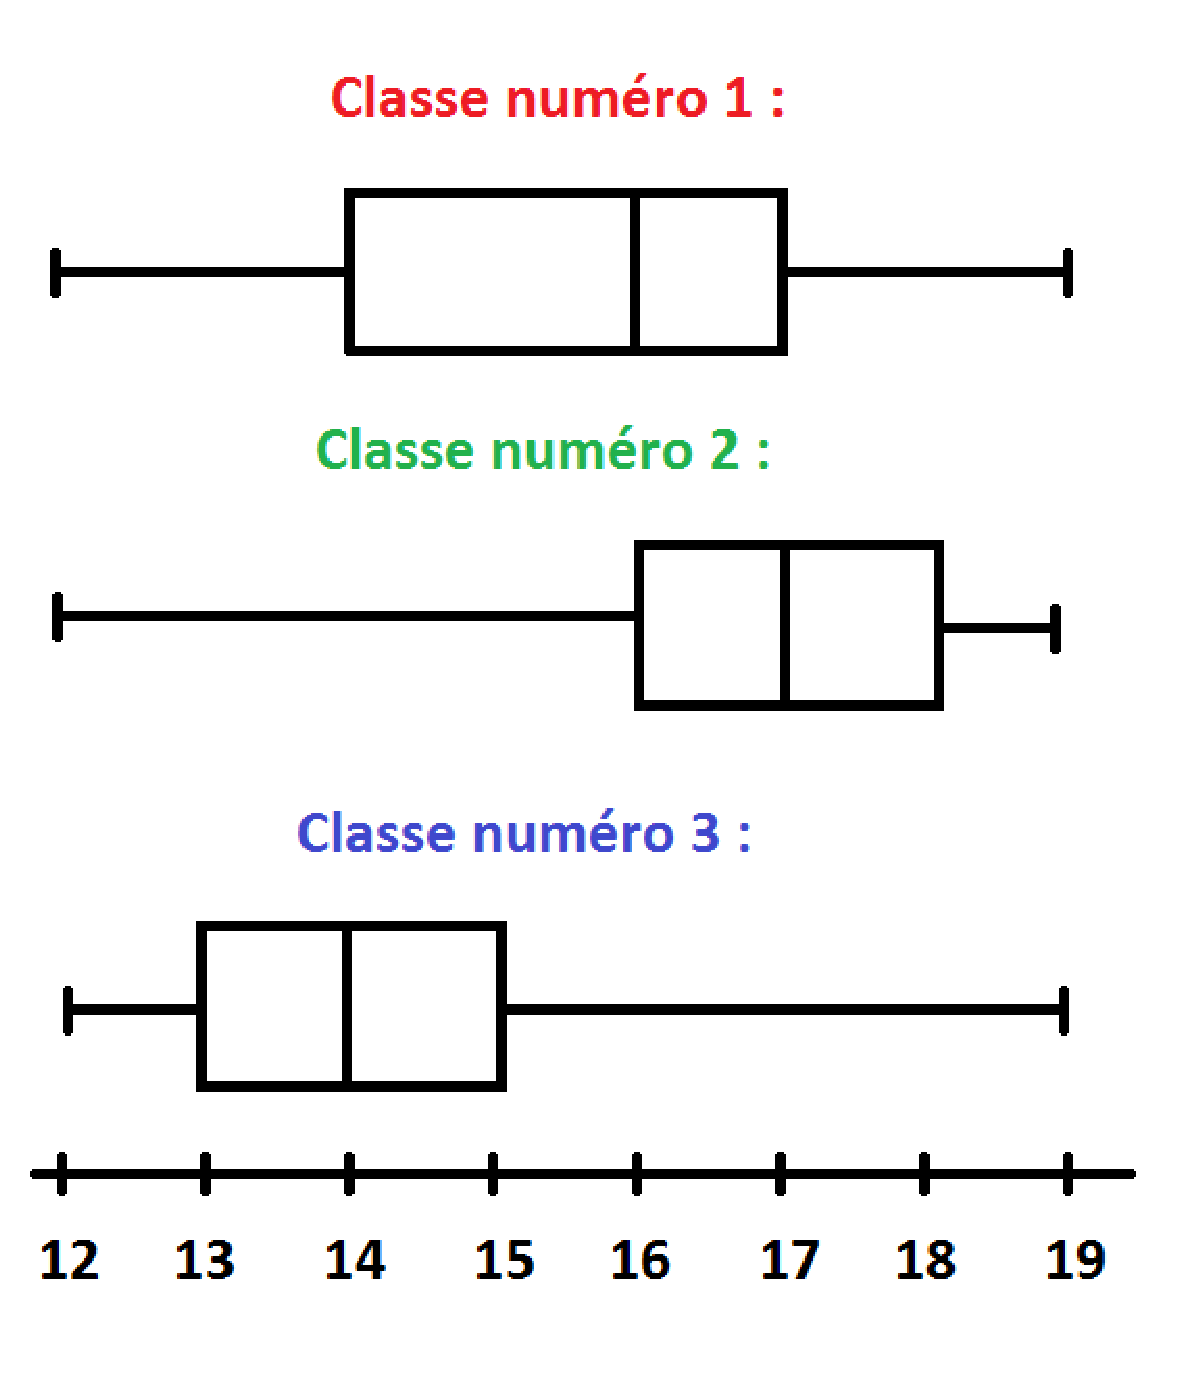
\includegraphics[scale=0.20]{boites.eps}
\end{center}


\end{exo}



\begin{exo}

\begin{enumerate}
\item La moyenne est plus élevée dans la classe 2, donc c'est celle qui a globalement le mieux réussi ce devoir.
\item L'écart-type est plus faible dans la classe 2, donc c'est celle dans laquelle les résultats ont été les plus homogènes.
\end{enumerate}


\end{exo}

\begin{exo}

Les écarts de température sont plus importants à Grenoble (climat continental) qu'à Quimper (climat océanique), donc c'est à Grenoble qu'il y a le plus grand écart-type des températures.
\end{exo}

\begin{exo}
\begin{enumerate}
\item Le débit moyen est plus important à Vernon ~: la courbe est plus haute.
\item L'écart-type du débit est  plus important à Vernon ~: il y a des variations plus importantes dans la courbe (elle est plus \og étirée \fg).
\end{enumerate}

\medskip

\textbf{Remarque~:} Vernon se trouve en aval d'Alfortville lorsqu'on suit le cours de la Seine. Cette dernière gagne les eaux de la Marne et de l'Oise entre les deux villes, ce qui fait que son débit est plus important à Vernon.
\end{exo}

\begin{exo}

La transformation
\[\text{Note}\mapsto 0,8\times\text{Note}+4\] peut être décomposée en deux étapes~:

\begin{itemize}
\item[\textbullet] \textbf{1\up{re} étape~:} On multiplie les notes par $0,8.$

\smallskip

Cela a pour effet de \og réduire \fg~{} la série, toutes les valeurs étant diminuées de 20~\%~: c'est le cas du minimum, de la moyenne, de la note maximale, etc. L'écart entre les notes est réduit de la même manière, ce qui fait fait que l'écart-type est multiplié lui aussi par $0,8.$


\begin{center}
\psset{xunit=0.75cm,yunit=1.0cm,algebraic=true,dimen=middle,dotstyle=o,dotsize=5pt 0,linewidth=2.pt,arrowsize=3pt 2,arrowinset=0.25}
\begin{pspicture*}(-4.800047660558245,0.4871814571342879)(18.007225511685323,2.7357858543977405)
\psline[linewidth=2.pt]{->}(-1.,2.)(6.,2.)
\psline[linewidth=2.pt]{->}(10.,2.)(16.,2.)
\rput[tl](-0.8886097594361083,1.39){Série de notes d'origine}
\rput[tl](6.5,1.39){Série après multiplication par $0,8$ $\implies$ données resserrées}
\psline[linewidth=2.pt](-4.,2.)(-1.,2.)
\psline[linewidth=2.pt](8.,2.)(10.4,2.)
\psdots[dotstyle=*,linecolor=blue](0.,2.)
\psdots[dotstyle=*,linecolor=blue](-2.,2.)
\psdots[dotstyle=*,linecolor=blue](-1.,2.)
\psdots[dotstyle=*,linecolor=blue](2.,2.)
\psdots[dotstyle=*,linecolor=blue](3.,2.)
\psdots[dotstyle=*,linecolor=red](9.6,2.)
\psdots[dotstyle=*,linecolor=red](10.4,2.)
\psdots[dotstyle=*,linecolor=red](11.2,2.)
\psdots[dotstyle=*,linecolor=red](12.8,2.)
\psdots[dotstyle=*,linecolor=red](13.6,2.)
\psdots[dotstyle=*,linecolor=blue](-4.,2.)
\psdots[dotstyle=*,linecolor=red](8.,2.)
\psdots[dotstyle=*,linecolor=blue](5.,2.)
\psdots[dotstyle=*,linecolor=red](15.2,2.)
\end{pspicture*}
\end{center}
\item[\textbullet] \textbf{2\up{e} étape~:} On ajoute $4$ points à chaque note.

\smallskip


Les notes sont \og décalées vers la droite \fg, mais l'écart entre elles ne change pas. Cela n'a donc pas d'effet sur l'écart-type.
\end{itemize}

\medskip

Conclusion~: seule la multiplication par $0,8$ a une incidence sur l'écart-type, qui devient
\[0,8\times 5=4.\]
\end{exo}


\setcounter{section}{15}

\section{Trigonométrie}

\setcounter{exo}{179}


\begin{exo}



\begin{enumerate}
\item ~{}


\begin{center}
\psset{xunit=1.0cm,yunit=1.0cm,algebraic=true,dimen=middle,dotstyle=o,dotsize=5pt 0,linewidth=2.pt,arrowsize=3pt 2,arrowinset=0.25}
\begin{pspicture*}(0.08,-0.44)(6.04,4.66)
\psline[linewidth=2.pt](1.,1.)(4.,1.)
\psline[linewidth=2.pt](2.5,1.12)(2.5,0.88)
\psline[linewidth=2.pt](4.,1.)(4.,4.)
\psline[linewidth=2.pt](3.88,2.5)(4.12,2.5)
\psline[linewidth=2.pt](4.,4.)(1.,4.)
\psline[linewidth=2.pt](2.5,3.88)(2.5,4.12)
\psline[linewidth=2.pt](1.,4.)(1.,1.)
\psline[linewidth=2.pt](1.12,2.5)(0.88,2.5)
\psline[linewidth=2.pt](1.,1.)(4.,4.)
\psline[linewidth=2.pt](1.,1.)(5.098076211353316,-0.09807621135331601)
\psline[linewidth=2.pt](3.031800099774507,0.5798139457331556)(2.9696835289499015,0.3479917474237798)
\psline[linewidth=2.pt](3.128392682403414,0.5539320412229037)(3.0662761115788086,0.322109842913528)
\psline[linewidth=2.pt](5.098076211353316,-0.09807621135331601)(4.,4.)
\psline[linewidth=2.pt](4.446067958777096,1.871607317596586)(4.677890157086472,1.9337238884211911)
\psline[linewidth=2.pt](4.4201860542668445,1.968199900225493)(4.652008252576221,2.0303164710500985)
\psline[linewidth=2.pt](4.,1.)(5.098076211353316,-0.09807621135331601)
\psline[linewidth=2.pt](4.,1.)(1.,4.)
\rput[bl](0.68,1.08){$K$}
\rput[bl](3.78,0.68){$L$}
\rput[bl](4.08,4.04){$M$}
\rput[bl](0.6,4.){$N$}
\rput[bl](5.18,-0.06){$O$}
\end{pspicture*}
\end{center}
\item On note $\Delta$ la médiatrice du segment $\left[MK\right].$ On rappelle que c'est~:
\begin{itemize}
\item[\textbullet] \textit{Définition.} La perpendiculaire à $\left[MK\right]$ passant par son milieu~;
\item[\textbullet] \textit{Caractérisation.} L'ensemble des points qui se trouvent à égale distance de $M$ et de $K.$
\end{itemize}

\medskip

$KLMN$ est un carré, donc $NK=NM~;$ et donc $N\in\Delta$ d'après la caractérisation ci-dessus. De même, $LK=LM,$ donc $L\in\Delta.$ Enfin $KOM$ est équilatéral, donc $OK=OM$ et par conséquent $O\in\Delta.$

Conclusion~: les points $O,L,N$ sont sur $\Delta,$ donc ils sont alignés.
\item $O,L,N$ étant alignés, $\widehat{OLN}=180^{\circ}.$ D'autre part, il est clair que $MLN$ est rectangle isocèle en $M,$ donc ses angles à la base sont égaux et l'on a $\widehat{MLN}=\frac{180^{\circ}-90^{\circ}}{2}=45^{\circ}.$

On en déduit $\widehat{MLO}=\widehat{OLN}-\widehat{MLN}=180^{\circ}-45^{\circ}=135^{\circ}.$
\end{enumerate}

\end{exo}




\begin{exo}


\begin{enumerate}
\item ~{}


\begin{center}
\newrgbcolor{ffxfqq}{1. 0.4980392156862745 0.}
\psset{xunit=1.0cm,yunit=1.0cm,algebraic=true,dimen=middle,dotstyle=o,dotsize=5pt 0,linewidth=2.pt,arrowsize=3pt 2,arrowinset=0.25}
\begin{pspicture*}(1.44,-1.38)(8.78,5.46)
\pscircle[linewidth=2.pt](5.,2.){3.}
\psline[linewidth=2.pt](2.,2.)(3.2903031230049153,4.465144334271982)
\psline[linewidth=2.pt](3.2903031230049153,4.465144334271982)(5.,2.)
\psline[linewidth=2.pt](4.215262386923419,3.3420457811203272)(4.01805084018166,3.2052700309607207)
\psline[linewidth=2.pt](4.2722522828232545,3.259874303311262)(4.075040736081497,3.1230985531516553)
\psline[linewidth=2.pt](3.2903031230049153,4.465144334271982)(8.,2.)
\pscustom[linewidth=2.pt,linecolor=ffxfqq,fillcolor=ffxfqq!20!white,fillstyle=solid,opacity=0.1]{
\parametricplot{0.0}{1.0885896065854297}{0.6*cos(t)+2.|0.6*sin(t)+2.}
\lineto(2.,2.)\closepath}
\pscustom[linewidth=2.pt,linecolor=ffxfqq,fillcolor=ffxfqq!20!white,fillstyle=solid,opacity=0.1]{
\parametricplot{-2.0530030470043634}{-0.9644134404189337}{0.6*cos(t)+3.2903031230049153|0.6*sin(t)+4.465144334271982}
\lineto(3.2903031230049153,4.465144334271982)\closepath}
\pscustom[linewidth=2.pt,linecolor=magenta,fillcolor=magenta!20!white,fillstyle=solid,opacity=0.1]{
\parametricplot{-0.9644134404189338}{-0.4822067202094669}{0.6*cos(t)+3.2903031230049153|0.6*sin(t)+4.465144334271982}
\lineto(3.2903031230049153,4.465144334271982)\closepath}
\pscustom[linewidth=2.pt,linecolor=magenta,fillcolor=magenta!20!white,fillstyle=solid,opacity=0.1]{
\parametricplot{2.6593859333803263}{3.141592653589793}{0.6*cos(t)+8.|0.6*sin(t)+2.}
\lineto(8.,2.)\closepath}
\rput[tl](7.46,4.52){$\mathcal{C}$}
\psline[linewidth=2.pt](2.,2.)(5.,2.)
\psline[linewidth=2.pt](3.45,2.12)(3.45,1.88)
\psline[linewidth=2.pt](3.55,2.12)(3.55,1.88)
\psline[linewidth=2.pt](5.,2.)(8.,2.)
\psline[linewidth=2.pt](6.45,2.12)(6.45,1.88)
\psline[linewidth=2.pt](6.55,2.12)(6.55,1.88)
\rput[bl](1.66,2.16){{$A$}}
\rput[bl](8.08,2.16){{$B$}}
\psdots[dotsize=4pt 0,dotstyle=*,linecolor=darkgray](5.,2.)
\rput[bl](5.08,2.16){{$I$}}
\rput[bl](3.08,4.64){{$M$}}
\end{pspicture*}
\end{center}

\item $\left[IA\right]$ et $\left[IM\right]$ sont deux rayons de $\mathcal{C},$ donc $IAM$ est isocèle en $I$ et ses angles à la base $\widehat{IAM}$ et $\widehat{AMI}$ sont égaux~:
\[\widehat{IAM}=\widehat{AMI}.\]

La démonstration est la même pour les deux autres angles grâce au triangle $IBM~:$

 \[\widehat{IMB}=\widehat{MBI}.\]
\item $\widehat{IAM}+\widehat{AMI}+\widehat{IMB}+\widehat{MBI}$ est la somme des angles du triangle $AMB,$ donc \[\widehat{IAM}+\widehat{AMI}+\widehat{IMB}+\widehat{MBI}=180^{\circ}.\]
\item D'après les questions 2 et 3~:
\[\underbrace{\widehat{IAM}+\widehat{AMI}}_{2\widehat{AMI}}+\underbrace{\widehat{IMB}+\widehat{MBI}}_{2\widehat{IMB}}=180^{\circ}.\]

En divisant par 2 l'égalité $2\widehat{AMI}+2\widehat{IMB}=180^{\circ},$ on obtient
\[\widehat{AMI}+\widehat{IMB}=90^{\circ}~;\] soit finalement 
\[\widehat{AMB}=90^{\circ}.\]
\end{enumerate}

\end{exo}

\begin{exo}%32


\medskip

$ABC$ est un triangle tel que $AB=3,$ $AC=4,$ $BC=5.$ On pose $\theta=\widehat{ACB}.$
\begin{enumerate}
\item ~{}


\begin{center}
\psset{xunit=1.0cm,yunit=1.0cm,algebraic=true,dimen=middle,dotstyle=o,dotsize=5pt 0,linewidth=2.pt,arrowsize=3pt 2,arrowinset=0.25}
\begin{pspicture*}(-5.02,-0.24)(0.16,5.6)
\psline[linewidth=2.pt](-4.,1.)(-1.,1.)
\psline[linewidth=2.pt](-4.,1.)(-4.,5.)
\psline[linewidth=2.pt](-4.,5.)(-1.,1.)
\pscustom[linewidth=2.pt,linecolor=magenta,fillcolor=magenta!20!white,fillstyle=solid,opacity=0.1]{
\parametricplot{-1.5707963267948966}{-0.9272952180016122}{0.6*cos(t)+-4.|0.6*sin(t)+5.}
\lineto(-4.,5.)\closepath}
\rput[tl](-3.8,4.28){\magenta{$\theta$}}
\rput[lt](-2.9,0.8){\parbox{1.8 cm}{~~~3 \\  (opp)}}
\rput[lt](-4.8,3.22){\parbox{1.8 cm}{~~~4 \\  (adj)}}
\rput[lt](-2.3,3.48){\parbox{1.8 cm}{~~~5 \\  (hyp)}}
\rput[bl](-4.36,0.98){$A$}
\rput[bl](-0.92,1.04){$B$}
\rput[bl](-4.3,4.98){$C$}
\end{pspicture*}
\end{center}

\[
\left.
    \begin{array}{ll}
        BC^2=5^2=25\\
        AB^2+AC^2=3^2+4^2=16+9=25
    \end{array}
\right \}BC^2=AB^2+AC^2.
\]

D'après \textbf{le théorème  réciproque de Pythagore}, $ABC$ est rectangle en $A.$

\item Dans $ABC$ rectangle en $A~:$
\[
\cos \theta=\frac{\text{adj}}{\text{hyp}}=\frac{4}{5}\qquad ,\qquad
\sin \theta=\frac{\text{opp}}{\text{hyp}}=\frac{3}{5}\qquad ,\qquad
\tan \theta=\frac{\text{opp}}{\text{adj}}=\frac{3}{4}.
\]
\item D'après la question précédente~:
\begin{align*}
\left(\cos\theta\right)^2+\left(\sin\theta\right)^2 &=\left(\frac{4}{5}\right)^2+\left(\frac{3}{5}\right)^2=\frac{4^2}{5^2}+\frac{3^2}{5^2}=\frac{16}{25}+ \frac{9}{25}= \frac{25}{25}=1\\
\frac{\sin\theta}{\cos\theta}&=\frac{\frac{3}{5}}{\frac{4}{5}}=\frac{3}{5}\times \frac{5}{4}=\frac{3}{4}=\tan \theta
\end{align*}
\end{enumerate}
\end{exo}

\begin{exo}

$ABC$ est un triangle rectangle en $A$ tel que $AB=4$ et $\widehat{BCA}=40^{\circ}.$ On note $H$ le pied de la hauteur issue de $A.$


\begin{center}
\psset{xunit=1.0cm,yunit=1.0cm,algebraic=true,dimen=middle,dotstyle=o,dotsize=5pt 0,linewidth=2.pt,arrowsize=3pt 2,arrowinset=0.25}
\begin{pspicture*}(0.28,1.98)(7.18,5.06)
\pspolygon[linewidth=2.pt,fillcolor=black!20!white,fillstyle=solid,opacity=0.1](2.793167869229448,4.1370142502787)(3.1181730014812694,3.864302563675473)(3.390884688084496,4.189307695927294)(3.0658795558326744,4.462019382530521)
\pspolygon[linewidth=2.pt,fillcolor=black!20!white,fillstyle=solid,opacity=0.1](3.490143624544604,2.)(3.490143624544604,2.424264068711929)(3.065879555832675,2.424264068711929)(3.065879555832675,2.)
\psline[linewidth=2.pt](1.,2.)(6.,2.)
\parametricplot{2.443460952792061}{3.141592653589793}{0.6*cos(t)+6.|0.6*sin(t)+2.}
\psline[linewidth=2.pt](6.,2.)(3.0658795558326744,4.462019382530521)
\psline[linewidth=2.pt](3.0658795558326744,4.462019382530521)(1.,2.)
\psline[linewidth=2.pt](3.0658795558326744,4.462019382530521)(3.065879555832675,2.)
\rput[bl](0.7,2.12){$B$}
\rput[bl](6.08,2.04){$C$}
\rput[bl](4.86,2.14){$40^{\circ}$}
\rput[bl](3.14,4.5){$A$}
\rput[bl](2.54,2.1){$H$}
\rput[bl](1.77,3.3){$4$}
\end{pspicture*}
\end{center}


On commence par la longueur $AC.$


Dans $ABC$ rectangle en $A~:$ \[\tan 40^{\circ}=\frac{\text{opp}}{\text{adj}}=\frac{4}{AC}.\]

On a donc $\tan 40^{\circ}\times AC=\frac{4}{\cancel{AC}}\times\cancel{AC},$ puis $\frac{\cancel{\tan 40^{\circ}}\times AC}{\cancel{\tan 40^{\circ}}}=\frac{4}{\tan 40^{\circ}}.$

Conclusion~: on obtient grâce à la calculatrice
\[AC=\frac{4}{\tan 40^{\circ}}\approx 4,77.\]

\medskip

Ensuite on calcule $AH.$


Dans $AHC$ rectangle en $H~:$ \[\sin 40^{\circ}=\frac{\text{opp}}{\text{hyp}}=\frac{AH}{AC}.\]

On a donc $\sin 40^{\circ}\times AC=\frac{AH}{\cancel{AC}}\times\cancel{AC},$ soit \[AH=\sin 40^{\circ}\times AC=\sin 40^{\circ}\times \frac{4}{\tan 40^{\circ}}\approx 3,06.\]

\medskip

\textbf{Remarque~:} Ne prenez pas de valeurs approchées dans les calculs intermédiaires, car les erreurs d'arrondis pourraient grossir au fur et à mesure des étapes de calcul, et même finir par \og exploser \fg. Si vous voulez un exemple, entrez la formule \og =1/3 \fg~{} dans la cellule $A1$ d'une feuille de calcul (un tableur). Vous obtenez $0,3333333\cdots$ Ensuite, vous entrez la formule \og =4*A1-1 \fg~{} dans la cellule A2, puis vous étirez vers le bas. En théorie, vous devriez toujours obtenir la même réponse, puisque $4\times\frac{1}{3}-1=\frac{4}{3}-\frac{3}{3}=\frac{1}{3}.$ Vous verrez que ce n'est pas du tout le cas, ce qui est dû à des problèmes d'arrondis.

\end{exo}


\begin{exo}



La différence d'altitude entre le haut et le bas de la piste est 
\[\np{2261}-\np{1839}=422~\text{m},\] si bien que l'on peut représenter la situation par la figure suivante~:



\begin{center}
\newrgbcolor{ffxfqq}{1. 0.4980392156862745 0.}
\newrgbcolor{xfqqff}{0.4980392156862745 0. 1.}
\psset{xunit=1.0cm,yunit=1.0cm,algebraic=true,dimen=middle,dotstyle=o,dotsize=5pt 0,linewidth=2.pt,arrowsize=3pt 2,arrowinset=0.25}
\begin{pspicture*}(1.56,0.7)(9.64,3.32)
\pspolygon[linewidth=2.pt,linecolor=xfqqff,fillcolor=xfqqff!20!white,fillstyle=solid,opacity=0.1](7.,1.4242640687119288)(6.575735931288071,1.4242640687119288)(6.575735931288071,1.)(7.,1.)
\psline[linewidth=2.pt](2.,1.)(7.,1.)
\psline[linewidth=2.pt](7.,1.)(7.,3.)
\psline[linewidth=2.pt](7.,3.)(2.,1.)
\rput[tl](7.32,2.06){422 m}
\pscustom[linewidth=2.pt,linecolor=ffxfqq,fillcolor=ffxfqq!20!white,fillstyle=solid,opacity=0.1]{
\parametricplot{0.0}{0.3805063771123649}{0.6*cos(t)+2.|0.6*sin(t)+1.}
\lineto(2.,1.)\closepath}
\rput[tl](2.85,1.3){\ffxfqq{$\theta$}}
\rput[tl](3.78,2.42){\np{1453}}
\end{pspicture*}
\end{center}


On nous demande de calculer la mesure de l'angle $\theta.$ On utilise le sinus~:
$\sin\theta=\frac{\text{opp}}{\text{hyp}}=\frac{422}{\np{1453}},$ donc $\theta\approx 16,9^{\circ}.$

\end{exo}

\begin{exo}%32

$ABC$ est un triangle équilatéral de côté 4, $H$ est le pied de la hauteur issue de $B.$

\begin{enumerate}
\item ~{}


\begin{center}
\newrgbcolor{ffxfqq}{1. 0.4980392156862745 0.}
\psset{xunit=1.0cm,yunit=1.0cm,algebraic=true,dimen=middle,dotstyle=o,dotsize=5pt 0,linewidth=2.pt,arrowsize=3pt 2,arrowinset=0.25}
\begin{pspicture*}(-3.62,0.5)(1.82,5.18)
\pspolygon[linewidth=2.pt,linecolor=magenta,fillcolor=magenta!20!white,fillstyle=solid,opacity=0.1](-1.,1.4242640687119283)(-1.4242640687119283,1.4242640687119283)(-1.4242640687119283,1.)(-1.,1.)
\psline[linewidth=2.pt](-3.,1.)(1.,1.)
\psline[linewidth=2.pt](-3.,1.)(-1.,4.464101615137754)
\psline[linewidth=2.pt](-1.,4.464101615137754)(1.,1.)
\psline[linewidth=2.pt](-1.,1.)(-1.,4.464101615137754)
\pscustom[linewidth=2.pt,linecolor=ffxfqq,fillcolor=ffxfqq!20!white,fillstyle=solid,opacity=0.1]{
\parametricplot{0.0}{1.0471975511965976}{0.6*cos(t)+-3.|0.6*sin(t)+1.}
\lineto(-3.,1.)\closepath}
\rput[bl](-3.36,1.06){$A$}
\rput[bl](1.08,1.16){$C$}
\rput[bl](-0.92,4.62){$B$}
\rput[bl](-0.92,1.16){$H$}
\rput[bl](-2.48,1.38){\ffxfqq{$60^{\circ}$}}
\end{pspicture*}
\end{center}

Le triangle $ABC$ est équilatéral, donc la hauteur $\left[HB\right]$ est aussi une médiane (propriété du collège) et $H$ est le milieu de $\left[AC\right].$ On a donc $AH=\frac{1}{2}\times 4=2.$ 

Ensuite on calcule $HB~:$ d'après le théorème de Pythagore dans le triangle rectangle $AHB,$ 
\[AH^2+HB^2=AB^2\hspace{0.8cm} 2^2+HB^2=4^2\hspace{0.8cm}4+HB^2=16\hspace{0.8cm}HB^2=16-4=12\hspace{0.8cm} HB=\sqrt{12}.\]
\item Dans $AHB$ rectangle en $H~:$

\begin{align*}
\cos 60^{\circ}&=\frac{\text{adj}}{\text{hyp}}=\frac{AH}{AB}=\frac{2}{4}=\frac{1}{2}\\
\sin 60^{\circ}&=\frac{\text{opp}}{\text{hyp}}=\frac{HB}{AB}=\frac{\sqrt{12}}{4}\\
\tan 60^{\circ}&=\frac{\text{opp}}{\text{adj}}=\frac{HB}{AH}=\frac{\sqrt{12}}{2}
\end{align*}

\medskip

\textbf{Remarque~:} le nombre $\frac{\sqrt{12}}{4}$ est mieux connu sous la forme $\frac{\sqrt{3}}{2},$ ce que l'on obtient par le calcul
\[\frac{\sqrt{12}}{4}=\frac{\sqrt{4\times 3}}{4}=\frac{\sqrt{4}\times\sqrt{3}}{4}=\frac{2\times\sqrt{3}}{4}=\frac{\cancel{2}\times\sqrt{3}}{\cancel{2}\times 2}=\frac{\sqrt{3}}{2}.\]

Avec le même calcul on trouve $\tan 60^{\circ}=\sqrt{3}.$
\end{enumerate}
\end{exo}

\begin{exo}

Chacun des cercles a pour rayon 1, donc le triangle $ABC$ est équilatéral de côté 4. C'est donc le triangle de l'exercice précédent (!), et l'on sait que sa hauteur $\left[HB\right]$ (en bleu) mesure $\sqrt{12}.$ Comme chaque segment vert mesure 1, on obtient
\[h=\sqrt{12}+2.\]


\begin{center}
\psset{xunit=1.0cm,yunit=1.0cm,algebraic=true,dimen=middle,dotstyle=o,dotsize=5pt 0,linewidth=2.pt,arrowsize=3pt 2,arrowinset=0.25}
\begin{pspicture*}(0.34,-0.32)(9.2,5.76)
\pscircle[linewidth=2.pt](2.,1.){1.}
\pscircle[linewidth=2.pt](4.,1.){1.}
\pscircle[linewidth=2.pt](6.,1.){1.}
\psline[linewidth=2.pt,linecolor=red](2.,1.)(6.,1.)
\psline[linewidth=2.pt,linecolor=red](2.,1.)(4.,4.464101615137754)
\psline[linewidth=2.pt,linecolor=red](4.,4.464101615137754)(6.,1.)
\pscircle[linewidth=2.pt](4.,4.464101615137754){1.}
\pscircle[linewidth=2.pt](3.,2.7320508075688767){1.}
\pscircle[linewidth=2.pt](5.,2.7320508075688767){1.}
\psline[linewidth=2.pt,linecolor=blue](4.,1.)(4.,4.464101615137754)
\rput[tl](1.64,1.14){\red{$A$}}
\rput[tl](6.14,1.06){\red{$C$}}
\rput[tl](3.54,4.7){\red{$B$}}
\psline[linewidth=2.pt,linecolor=green](4.,4.464101615137754)(4.020918147942029,5.463882806742535)
\psline[linewidth=2.pt,linecolor=green](4.,1.)(4.,0.)
\rput[tl](3.5,0.84){\red{$H$}}
\psline[linewidth=2.pt]{->}(8.,3.)(8.,5.46)
\psline[linewidth=2.pt]{->}(8.,3.)(8.,0.)
\rput[tl](8.12,2.62){$h$}
\end{pspicture*}
\end{center}

\end{exo}

\begin{exo}

Commençons par une remarque~: 

La figure ci-dessous représente un quart de cercle de rayon $R,$ dans lequel on a tracé un angle de $60^{\circ}.$ Dans un exercice précédent, on a vu que $\cos 60^{\circ}=\frac{1}{2}.$ Pour notre figure, cela signifie que le rapport $\frac{\text{adj}}{\text{hyp}}=\frac{OH}{OM}$ est égal à $\frac{1}{2}.$ Mais $OM$ est le rayon $R$ du quart de cercle, et $MN=OH~;$ on en déduit donc que $\frac{OH}{OM}=\frac{MN}{R}=\frac{1}{2}~;$ c'est-à-dire que la longueur $MN$ est deux fois plus petite que le rayon $R.$


\begin{center}
\newrgbcolor{ffxfqq}{1. 0.4980392156862745 0.}
\psset{xunit=1.0cm,yunit=1.0cm,algebraic=true,dimen=middle,dotstyle=o,dotsize=5pt 0,linewidth=2.pt,arrowsize=3pt 2,arrowinset=0.25}
\begin{pspicture*}(1.18,0.34)(6.88,5.56)
\pspolygon[linewidth=2.pt,linecolor=magenta,fillcolor=magenta!20!white,fillstyle=solid,opacity=0.1](4.,1.424264068711929)(3.575735931288071,1.424264068711929)(3.575735931288071,1.)(4.,1.)
\pspolygon[linewidth=2.pt,linecolor=magenta,fillcolor=magenta!20!white,fillstyle=solid,opacity=0.1](2.,4.039837546425826)(2.424264068711929,4.039837546425826)(2.424264068711929,4.464101615137754)(2.,4.464101615137754)
\psline[linewidth=2.pt](2.,1.)(6.,1.)
\psline[linewidth=2.pt](2.,1.)(2.,5.)
\parametricplot[linewidth=2.pt]{0.0}{1.5707963267948966}{1.*4.*cos(t)+0.*4.*sin(t)+2.|0.*4.*cos(t)+1.*4.*sin(t)+1.}
\pscustom[linewidth=2.pt,linecolor=ffxfqq,fillcolor=ffxfqq!20!white,fillstyle=solid,opacity=0.1]{
\parametricplot{0.0}{1.0471975511965976}{0.6*cos(t)+2.|0.6*sin(t)+1.}
\lineto(2.,1.)\closepath}
\psline[linewidth=2.pt](2.,1.)(4.,4.464101615137754)
\psline[linewidth=2.pt](4.,4.464101615137754)(4.,1.)
\psline[linewidth=2.pt](2.,4.464101615137754)(4.,4.464101615137754)
\rput[tl](2.66,0.9){$\text{adj}$}
\rput[tl](2.3,3.3){\parbox{1.8 cm}{$\text{hyp}$ \\ $~=R$}}
\rput[tl](4.06,2.9){$\text{opp}$}
\rput[bl](1.6,0.98){$O$}
\rput[bl](4.08,4.5){$M$}
\rput[bl](2.54,1.4){\ffxfqq{$60\textrm{\degre}$}}
\rput[bl](4.1,1.16){$H$}
\rput[bl](1.6,4.24){$N$}
\end{pspicture*}
\end{center}

\medskip

Revenons à l'exercice~: on peut assimiler la terre a une sphère de périmètre \np{40000}~km\footnote{Rappelons qu'à l'origine, le mètre a été défini comme 1/\np{40000000}\up{e} du périmètre de la terre. La valeur \np{40000} est donc une excellente approximation.}, donc l'équateur mesure \np{40000}~km de long. Dans le dessin de la terre de profil ci-dessous, cela correspond au périmètre du cercle de rayon $R$ (en bleu).



\begin{center}
\newrgbcolor{ududff}{0.30196078431372547 0.30196078431372547 1.}
\newrgbcolor{ffxfqq}{1. 0.4980392156862745 0.}
\psset{xunit=1.0cm,yunit=1.0cm,algebraic=true,dimen=middle,dotstyle=o,dotsize=5pt 0,linewidth=2.pt,arrowsize=3pt 2,arrowinset=0.25}
\begin{pspicture*}(-0.4939401124587409,-1.0617758441584468)(6.463013697570776,5.410299366990214)
\pscircle[linewidth=2.pt](3.,2.){3.}
\psline[linewidth=2.pt,linecolor=ududff](0.,2.)(6.,2.)
\rput[tl](4.35,1.847495749126619){\ududff{$R$}}
\psline[linewidth=2.pt,linecolor=red](1.5029398763527315,4.599771333441698)(4.497060123647269,4.599771333441698)
\psline[linewidth=2.pt](3.,-1.)(3.,5.)
\pscustom[linewidth=2.pt,linecolor=ffxfqq,fillcolor=ffxfqq!20!white,fillstyle=solid,opacity=0.1]{
\parametricplot{0.0}{1.0483287409877216}{0.6324503463663198*cos(t)+3.|0.6324503463663198*sin(t)+2.}
\lineto(3.,2.)\closepath}
\psline[linewidth=2.pt](3.,2.)(4.497060123647269,4.599771333441698)
\psdots[dotstyle=*,linecolor=ududff](3.,2.)
\psdots[dotstyle=*,linecolor=ududff](0.,2.)
\psdots[dotstyle=*,linecolor=ududff](6.,2.)
\psdots[dotstyle=*,linecolor=red](3.,4.599771333441698)
\psdots[dotsize=4pt 0,dotstyle=*,linecolor=red](1.5029398763527315,4.599771333441698)
\psdots[dotsize=4pt 0,dotstyle=*,linecolor=red](4.497060123647269,4.599771333441698)
\psdots[dotsize=4pt 0,dotstyle=*,linecolor=darkgray](3.,5.)
\psdots[dotsize=4pt 0,dotstyle=*,linecolor=darkgray](3.,-1.)
\rput[bl](3.6,2.4){\ffxfqq{$60^{\circ}$}}
\end{pspicture*}
\end{center}

D'après la remarque faite au début de l'exercice, le cercle que l'on parcourt lorsqu'on fait le tour de la terre à $60^{\circ}$ de latitude nord a un rayon (en rouge) deux fois plus petit que celui du cercle à l'équateur.

\medskip

Le cercle rouge ayant un rayon deux fois plus petit que celui du cercle bleu, son périmètre est aussi deux fois plus petit que celui du cercle bleu\footnote{Il y a proportionnalité entre rayon et périmètre d'après la formule $P=2\pi R.$}~; il mesure donc \np{20000}~km.

\medskip


Conclusion~: lorsqu'on fait le tour de la terre en restant à $60^{\circ}$ de latitude nord, on parcourt \np{20000}~km.

\end{exo}


\begin{exo}

$AHC$ est un triangle rectangle en $H.$ La droite passant par $A$ et perpendiculaire à la droite $(AC)$ coupe la droite $(HC)$ en $B.$

On sait que $AH=4,8$ et que $HC=6,4.$


\begin{center}
\psset{xunit=0.6cm,yunit=0.6cm,algebraic=true,dimen=middle,dotstyle=o,dotsize=5pt 0,linewidth=1.6pt,arrowsize=3pt 2,arrowinset=0.25}
\begin{pspicture*}(-6.76,-0.3)(4.88,5.44)
\pspolygon[linewidth=2.pt,fillcolor=black!20!white,fillstyle=solid,opacity=0.1](-2.6545584412271577,4.460588745030456)(-2.315147186257615,4.2060303038033)(-2.060588745030458,4.5454415587728425)(-2.4,4.8)
\pspolygon[linewidth=2.pt,fillcolor=black!20!white,fillstyle=solid,opacity=0.1](-1.9757359312880722,0.)(-1.9757359312880722,0.4242640687119286)(-2.4,0.4242640687119286)(-2.4,0.)
\psline[linewidth=2.pt](-2.4,4.8)(4.,0.)
\psline[linewidth=2.pt](-2.4,0.)(-2.4,4.8)
\psline[linewidth=2.pt](-6.,0.)(-2.4,4.8)
\psline[linewidth=2.pt](-6.,0.)(4.,0.)
\rput[bl](4.08,0.16){{$C$}}
\rput[bl](-3.2,0.36){{$H$}}
\rput[bl](-3,4.84){{$A$}}
\rput[bl](-6.4,0.2){{$B$}}
\end{pspicture*}
\end{center}

\begin{enumerate}
\item La somme des angles du triangle $ABC$ vaut $180^{\circ},$ donc \begin{equation}\label{A}\widehat{ACH}+\widehat{HBA}=180^{\circ}-\widehat{BAC}=180^{\circ}-90^{\circ}=90^{\circ}.
\end{equation}

%On dit que $\widehat{ACH}$ et $\widehat{HBA}$ sont complémentaires (leur somme vaut $90^{\circ}$).

\medskip

On raisonne de la même façon dans le triangle $BAH~:$
 \begin{equation}\label{B}\widehat{BAH}+\widehat{HBA}=180^{\circ}-\widehat{AHB}=180^{\circ}-90^{\circ}=90^{\circ}.
\end{equation}

%Les angles $\widehat{BAH}$ et $\widehat{HBA}$ sont aussi complémentaires.

\medskip

On compare les égalités (\ref{A}) et (\ref{B})~:

\[\widehat{ACH}+\widehat{HBA}=90^{\circ}\qquad\text{et}\qquad\widehat{BAH}+\widehat{HBA}=90^{\circ},\] donc \[\widehat{ACH}=\widehat{BAH}.\]
\item Dans $ACH$ rectangle en $H~:$
\[\tan \widehat{ACH}=\frac{\text{opp}}{\text{adj}}=\frac{AH}{HC}=\frac{4,8}{6,4}=\frac{48}{64}=\frac{\cancel{16}\times 3}{\cancel{16}\times 4}=\frac{3}{4}.\]
\item On sait que $\widehat{ACH}=\widehat{BAH},$ donc comme $\tan \widehat{ACH}=\frac{3}{4},$ on a aussi $\tan \widehat{BAH}=\frac{3}{4}.$

Mais dans le triangle $BAH$ rectangle en $H,$

\[\tan \widehat{BAH}=\frac{\text{opp}}{\text{adj}}=\frac{BH}{AH}=\frac{BH}{4,8}.\]

On a donc $\frac{3}{4}=\frac{BH}{4,8},$ puis $BH=\frac{3}{4}\times 4,8=3\times\frac{4,8}{4}=3\times 1,2=3,6.$
\end{enumerate}


\end{exo}

\setcounter{section}{10}



\section{Systèmes et équations de droites}


\setcounter{exo}{135}


\begin{exo}

\begin{enumerate}
\item 

On multiplie la deuxième ligne par 2 et on laisse la première inchangée~:

\[
\systeme*{8x+6y=26\qquad\textcolor{red}{~(\times 1)},5x-3y=-31\qquad\textcolor{red}{~(\times 2)}}
\]

\[
\systeme*{8x+6y=26,10x-6y=-62}
\]

On ajoute membre à membre et on résout l'équation en $x~:$

\begin{align*}8x+\cancel{6y}+10x-\cancel{6y}&=26-62\\
\frac{\cancel{18}x}{\cancel{18}}&=\frac{-36}{18}\\
x&=-2.\end{align*}

On remplace dans la première ligne pour trouver $y~:$

\begin{align*}
8\times (-2)+6y&=26\\
-16+6y&=26\\
\cancel{-16}+6y+\cancel{16}&=26+16\\
\frac{\cancel{6}y}{\cancel{6}}&=\frac{42}{6}\\
y&=7.\end{align*}

On vérifie la solution trouvée~:
\begin{align*}8\times (-2)+6\times 7&=26\\5\times (-2)-3\times 7&=-31.\end{align*}


Conclusion~: la solution du système est $(x,y)=(-2,7).$
\item On multiplie la première ligne par 2 et la deuxième par $-3~:$

\[
\systeme*{9x+2y=17\qquad\textcolor{red}{~(\times 2)},6x+5y=-7\qquad\textcolor{red}{~(\times (-3))}}
\]

\[
\systeme*{18x+4y=34,-18x-15y=21}
\]

On ajoute membre à membre et on résout l'équation en $y~:$

\begin{align*}\cancel{18x}+4y-\cancel{18x}-15y&=34+21\\
\frac{\cancel{-11}y}{\cancel{-11}}&=\frac{55}{-11}\\
y&=-5.\end{align*}

On remplace dans la première ligne pour trouver $x~:$

\begin{align*}
9x+2\times (-5)&=17\\
9x-10&=17\\
9x-\cancel{10}+\cancel{10}&=17+10\\
\frac{\cancel{9}x}{\cancel{9}}&=\frac{27}{9}\\
x&=3.\end{align*}

On vérifie la solution trouvée~:
\begin{align*}9\times 3+2\times (-5)&=17\\6\times 3+5\times (-5)&=-7.\end{align*}


Conclusion~: la solution du système est $(x,y)=(3,-5).$
\end{enumerate}

\end{exo}

\begin{exo}


On note~:

\begin{itemize}
\item[\textbullet] $x$ le nombre d'objets A fabriqués~;
\item[\textbullet] $y$ le nombre d'objets B fabriqués.
\end{itemize}

\medskip

On a fabriqué 45 objets, donc $x+y=45.$ On a utilisé 163~kg de bois, donc $3x+5y=163.$ L'énoncé se traduit donc par le système~:

\[
\systeme*{x+y=45,3x+5y=163}
\]

On multiplie la première ligne par $-3$ et on laisse la deuxième identique~:

\[
\systeme*{x+y=45\qquad \textcolor{red}{\qquad (\times (-3))},3x+5y=163 \qquad \textcolor{red}{\qquad (\times 1)}}
\]
\[
\systeme*{-3x-3y=-135,3x+5y=163}
\]
Puis on ajoute membre à membre les deux lignes et on en déduit la valeur de $y~:$
\begin{align*}
\cancel{-3x}-3y+\cancel{3x}+5y&=-135+163\\
\frac{\cancel{2}y}{\cancel{2}}&=\frac{28}{2}\\
y&=14.\end{align*} 
Puis en reprenant la première ligne du système de départ~:
\begin{align*}
x+y&=45\\
14+y&=45\\
\cancel{14}+y-\cancel{14}&=45-14\\
y&=31.\end{align*}

\medskip

Ici, il est inutile de vérifier la solution, car on est sûr dès le départ qu'il en existe une (les objets ont été fabriqués~!).

Conclusion~: la solution est $x=14,$ $y=31.$ Autrement dit, on a fabriqué 14 objets de type A et 31 objets de type B.

\end{exo}

\begin{exo}


On note~:

\begin{itemize}
\item[\textbullet] $d_1$ la distance (exprimée en mètres) à la mairie la plus proche de l'auto-stoppeur~;
\item[\textbullet] $d_2$ la distance (exprimée en mètres) à la mairie la plus éloignée.
\end{itemize}

\medskip


\begin{center}
\newrgbcolor{ududff}{0.30196078431372547 0.30196078431372547 1.}
\newrgbcolor{xfqqff}{0.4980392156862745 0. 1.}
\newrgbcolor{ffxfqq}{1. 0.4980392156862745 0.}
\psset{xunit=1.0cm,yunit=0.5cm,algebraic=true,dimen=middle,dotstyle=o,dotsize=5pt 0,linewidth=2.pt,arrowsize=3pt 2,arrowinset=0.25}
\begin{pspicture*}(-4.4044015326652195,0.2)(11.303675040729676,4.087281269203539)
\psline[linewidth=2.pt](-3.,3.)(9.,3.)
\psline[linewidth=2.pt,linecolor=green]{->}(-2.,2.)(-3.,2.)
\psline[linewidth=2.pt,linecolor=green]{->}(1.,2.)(2.,2.)
\psline[linewidth=2.pt,linecolor=xfqqff]{->}(5.,2.)(2.,2.)
\psline[linewidth=2.pt,linecolor=xfqqff]{->}(6.,2.)(9.,2.)
\rput[tl](-3.508503629239655,4){\ududff{Mairie 1}}
\rput[tl](8.396984065171177,4){\ududff{Mairie 2}}
\rput[tl](0.911259360993129,4){\ffxfqq{Auto-stoppeur}}
\psline[linewidth=2.pt,linecolor=green](-2.,2.)(-1.,2.)
\psline[linewidth=2.pt,linecolor=green](1.,2.)(0.,2.)
\rput[tl](-0.7,2.3){\green{$d_1$}}
\rput[tl](5.3,2.3){\xfqqff{$d_2$}}
\psline[linewidth=2.pt,linecolor=green]{->}(6.,1.)(4.,1.)
\psline[linewidth=2.pt,linecolor=green]{->}(7.,1.)(9.,1.)
\rput[tl](6.3,1.3){\green{$d_1$}}
\psline[linewidth=2.pt,linecolor=red]{->}(3.,1.)(2.,1.)
\psline[linewidth=2.pt,linecolor=red]{->}(3.,1.)(4.,1.)
\rput[tl](2.7030551678442576,0.75){\red{340}}
\begin{scriptsize}
\psdots[dotstyle=*,linecolor=ududff](-3.,3.)
\psdots[dotstyle=*,linecolor=ududff](9.,3.)
\psdots[dotstyle=*,linecolor=ffxfqq](2.,3.)
\end{scriptsize}
\end{pspicture*}
\end{center}


\begin{itemize}
\item[\textbullet] La distance totale (en mètres) entre les deux mairies est \[d_1+d_2=\np{3000}.\]
\item[\textbullet] Le son émis par le carillon de la Mairie 1 met une seconde de moins pour arriver jusqu'à l'auto-stoppeur que le son émis par le carillon de la Mairie 2. Autrement dit, quand le son émis par le carillon de la Mairie 1 arrive à l'auto-stoppeur, il reste 340 mètres à parcourir au son qui vient du carillon de la Mairie 2.\footnote{On utilise le fait que le son parcourt 340 mètres en 1 seconde.} Finalement~:
\[d_2=d_1+340.\]
\end{itemize}

\medskip

Le problème se traduit donc par le système

\[
\systeme*{d_1+d_2=\np{3000},d_2=d_1+340}
\]

On présente sous la forme habituelle~:

\[
\systeme*{d_1+d_2=\np{3000},-d_1+d_2=340}
\]

On ajoute membre à membre (il est inutile de multiplier les lignes par des nombres, les $d_1$ vont s'éliminer)~:

\begin{align*}\cancel{d_1}+d_2-\cancel{d_1}+d_2&=\np{3000}+340\\
\frac{\cancel{2}d_2}{\cancel{2}}&=\frac{\np{3340}}{2}\\
d_2&=\np{1670}
\end{align*}

Conclusion~: l'auto-stoppeur est à \np{1670} mètres de la Mairie 2, et à $\np{3000}-\np{1670}=\np{1330}$ mètres de la Mairie 1.

\end{exo}



\begin{exo}


\begin{enumerate}
\item A l'aller, il y a 2 locomotives et 10 wagons-citernes, pour une longueur totale de 152~m. On a donc
\[2x+10y=152.\] Au retour, il y a 1 locomotive et 12 wagons-citernes, pour une longueur de 160~m. On a donc \[1x+12y=160.\] L'énoncé se traduit donc par le système

\[
\systeme*{2x+10y=152,x+12y=160}
\]
\item On multiplie la deuxième ligne par $-2~:$
\[
\systeme*{2x+10y=152,x+12y=160\textcolor{red}{\qquad\times (-2)}}
\]
\[
\systeme*{2x+10y=152,-2x-24y=-320}
\]
Puis on ajoute membre à membre les deux lignes~:
\[
2x+10y-2x-24y=152-320.\] Les $x$ se simplifient~:
\[-14y=-168.\] On en déduit
\[\frac{\cancel{-14}y}{\cancel{-14}}=\frac{-168}{-14}\hspace{2cm}y=12.\]
Puis en reprenant la deuxième ligne du système de départ~:
\begin{align*}
x+12y&=160\\
x+12\times 12&=160\\
x+144&=160\\
x+\cancel{144}-\cancel{144}&=160-144\\
x&=16.\end{align*}

\medskip

Ici, il est inutile de vérifier la solution, car on est sûr dès le départ qu'il en existe une (les locomotives et les wagons-citernes ont une longueur~!).

\medskip

Conclusion~: les locomotives mesurent 16~m de long, et les wagons-citernes 12~m.

\end{enumerate}

\end{exo}



\begin{exo}

On exprimera les distances en m et le temps en s.% et les vitesses en m/s.

\medskip

Je note $v_1$ ma vitesse propre en m/s (c'est-à-dire la vitesse que j'aurais sans tapis roulant), et $v_2$ la vitesse du tapis roulant (en m/s également).

\medskip

À l'aller, dans le sens du tapis, je parcours 15~m en 5~s, donc j'avance à $15\div 3=5$~m/s.
Cette vitesse est la somme de $v_1$ et $v_2,$ soit
\[v_1+v_2=3.\]
Au retour, en sens contraire, je parcours 5~m en 5~s, donc j'avance à $1$~m/s.
Cette vitesse est la différence de $v_1$ et $v_2,$ soit
\[v_1-v_2=1.\]

On a donc le système
\[
\systeme*{v_1+v_2=3,v_1-v_2=1}
\]

Il n'est pas nécessaire de résoudre le système dans son intégralité, puisqu'on nous demande seulement la vitesse $v_2$ du tapis roulant. Pour aller au plus vite, on multiplie la deuxième ligne par $(-1)$ et on ajoute membre à membre~:

\[
\systeme*{v_1+v_2=3,v_1-v_2=1\textcolor{red}{\qquad\times (-1)}}
\]
\[
\systeme*{v_1+v_2=3,-v_1+v_2=-1}
\]
On obtient \begin{align*}
\cancel{v_1}+v_2-\cancel{v_1}+v_2&=3-1\\
\frac{\cancel{2}v_2}{\cancel{2}}&=\frac{2}{2}\\
v_2&=1.\end{align*}
Conclusion~: le tapis roulant avance à la vitesse de 1~m/s.


\end{exo}

\begin{exo}


\begin{enumerate}
\item On écrit les équations sous forme cartésienne~:
\begin{alignat*}{2}
&D:y=2x-4\qquad \qquad &&D':x=3\\
&D:-2x+1y+4=0\qquad\qquad &&D':1x+0y-3=0\end{alignat*}
\item On écrit les équations sous forme réduite~:
\begin{alignat*}{2}
&\Delta:-5x+y+3=0\qquad\qquad &&\Delta':3x+4y=0\\
&\Delta:y=5x-3\qquad\qquad &&\Delta':4y=-3x\\
& &&\Delta':y=-\frac{3}{4}x
\end{alignat*}

\end{enumerate}

\end{exo}


\begin{exo}

\begin{enumerate}
\item On écrit les équations de droites sous forme réduite pour pouvoir les tracer~:

\begin{alignat*}{2}
&D_1:3x+2y-5=0\qquad\qquad &&D_2:-x+y+3=0\\
&D_1:2y=-3x+5\qquad\qquad &&D_2:y=x-3\\
&D_1:y=\frac{-3x+5}{2} && \\
\end{alignat*}

\setlength{\columnseprule}{0.5pt}
\begin{multicols}{2}

\underline{Tracé de $D_1.$}

\medskip

\begin{center}
 \begin{tabular}{|c|c|c|}\hline
$x$& $0$ &$2$ \\ \hline 
$y$&$2,5$ &$-0,5$  \\ \hline
\end{tabular}
\end{center}


\begin{align*}&\frac{-3\times 0+5}{2}=\frac{5}{2}=2,5\\
&\frac{-3\times 2+5}{2}=\frac{-1}{2}=-0,5
\end{align*}

\columnbreak

\underline{Tracé de $D_2.$}

\medskip
\begin{center}
 \begin{tabular}{|c|c|c|}\hline
$x$& $0$ &$2$ \\ \hline 
$y$&$-3$ &$-1$  \\ \hline
\end{tabular}
\end{center}


\begin{align*}&0-3=-3\\
&2-3=-1
\end{align*}

\end{multicols}


\begin{center}
\newrgbcolor{ududff}{0.30196078431372547 0.30196078431372547 1.}
\psset{xunit=1.0cm,yunit=1.0cm,algebraic=true,dimen=middle,dotstyle=o,dotsize=5pt 0,linewidth=2.pt,arrowsize=3pt 2,arrowinset=0.25}
\begin{pspicture*}(-2.26,-4.38)(5.64,4.26)
\multips(0,-4)(0,1.0){9}{\psline[linestyle=dashed,linecap=1,dash=1.5pt 1.5pt,linewidth=0.4pt,linecolor=lightgray]{c-c}(-2.26,0)(5.64,0)}
\multips(-2,0)(1.0,0){8}{\psline[linestyle=dashed,linecap=1,dash=1.5pt 1.5pt,linewidth=0.4pt,linecolor=lightgray]{c-c}(0,-4.38)(0,4.26)}
\psaxes[labelFontSize=\scriptstyle,xAxis=true,yAxis=true,Dx=1.,Dy=1.,ticksize=-2pt 0,subticks=2]{->}(0,0)(-2.26,-4.38)(5.64,4.26)
\psplot[linewidth=2.pt,linecolor=ududff]{-2.26}{5.64}{(--5.-3.*x)/2.}
\rput[tl](-1.44,3.46){\ududff{$D_1$}}
\psplot[linewidth=2.pt,linecolor=red]{-2.26}{5.64}{(-6.--2.*x)/2.}
\rput[tl](2.96,0.8){\red{$D_2$}}
\begin{scriptsize}
\psdots[dotstyle=*,linecolor=ududff](0.,2.5)
\psdots[dotstyle=*,linecolor=ududff](2.,-0.5)
\psdots[dotstyle=*,linecolor=red](0.,-3.)
\psdots[dotstyle=*,linecolor=red](2.,-1.)
\end{scriptsize}
\end{pspicture*}
\end{center}

\item Pour déterminer les coordonnées du point d'intersection des droites $D_1$ et $D_2,$ on résout le système~:

\[
\systeme*{3x+2y-5=0,-x+y+3= 0}\qquad\qquad \systeme*{3x+2y=5,-x+y=-3}\begin{matrix}\textcolor{red}{(\times 1)}\\ \textcolor{red}{(\times 3)}\end{matrix}\qquad\qquad \systeme*{3x+2y=5,-3x+3y=-9}
\]

\medskip


On ajoute membre à membre les deux lignes. Les $x$ s'éliminent. On obtient une équation du premier degré en $y,$ que l'on résout~:



\begin{align*}
\cancel{3x}+2y-\cancel{3x}+3y&=5-9\\
\frac{\cancel{5}y}{\cancel{5}}&=\frac{-4}{5}\\
y&=-0,8.\end{align*}

\medskip


On reprend la première ligne du système pour trouver $x~:$



\begin{align*}
3x+2y-5&=0\\
3x+2\times (-0,8)-5&=0\\
3x-1,6-5&=0\\
3x-6,6&=0\\
3x-\cancel{6,6}+\cancel{6,6}&=0+6,6\\
\frac{\cancel{3}x}{\cancel{3}}&=\frac{6,6}{3}\\
x&=2,2.\end{align*}
\end{enumerate}


\medskip

Enfin on vérifie que le couple $(x,y)=(2,2;-0,8)$ est bien solution du système~:


\[
\left \{
\begin{array}{c @{=} c}
    3\times 2,2+2\times(-0,8) -5& 0 \\
    -2,2+(-0,8)+3 & 0 \\
\end{array}
\right.
\]

\medskip

Conclusion~: les droites $D_1$ et $D_2$ se coupent au point de coordonnées $(2,2;-0,8).$

\medskip

\textbf{Remarques~:}

\begin{itemize}
\item[\textbullet] On aurait aussi pu utiliser la méthode de la leçon sur les équations de droites et résoudre l'équation
\[\frac{-3x+5}{2}=x-3\] (on rappelle que cela permet de trouver $x~;$ et qu'il faut ensuite remplacer dans l'une des deux équations de droites pour trouver $y$).
\item[\textbullet] Si la plupart des systèmes d'équations ont une unique solution, c'est que leur résolution revient à chercher les points d'intersection de deux droites~; et que lorsque les droites ne sont pas parallèles, il n'y a qu'un seul point d'intersection\footnote{Lorsque les droites sont parallèles, soit elles sont confondues et le système a une infinité de solutions (correspondant à tous les points de la droite)~; soit les droites sont parallèles et distinctes, et alors le système n'a aucune solution. Un exemple est $\systeme*{2x+y=4,2x+y=5},$ qui n'a clairement aucune solution, puisque quel que soit le couple $(x,y),$ $2x+y$ ne peut pas être égal à la fois à 4 et à 5. En transposant, on obtient les droites d'équations $y=-2x+4$ et $y=-2x+5,$ qui sont parallèles puisqu'elles ont le même coefficient directeur ($-2$), mais qui sont distinctes puisque leurs ordonnées à l'origine différent (4 pour l'une, 5 pour l'autre).}.
\end{itemize}

\end{exo}






\begin{exo}


\begin{enumerate}
\item On note $\Delta$ la perpendiculaire à $(BC)$ passant par $A.$ Le vecteur 

\[\overrightarrow{BC}\begin{pmatrix} x_C-x_B\\y_C-y_B \end{pmatrix}\qquad \overrightarrow{BC}\begin{pmatrix} 5-2\\-2-4 \end{pmatrix}\qquad \overrightarrow{BC}\begin{pmatrix} 3\\-6 \end{pmatrix}\]
est perpendiculaire à $\Delta,$ donc d'après le théorème admis dans le cadre avant l'énoncé, $\Delta$ a une équation cartésienne de la forme
\[3x+(-6)y+c=0.\]
De plus $\Delta$ passe par $A(-1;0),$ donc $3\times (-1)+(-6)\times 0+c=0,$ soit $-3+c=0~;$ et donc $c=3.$ On a donc finalement
\[\Delta:3x-6y+3=0.\]

\medskip

\textbf{Remarque~:} On peut diviser par $3,$ pour avoir quelque chose de plus \og léger \fg~:
\[\Delta:x-2y+1=0.\]


\begin{center}
\newrgbcolor{xfqqff}{0.4980392156862745 0. 1.}
\newrgbcolor{ududff}{0.30196078431372547 0.30196078431372547 1.}
\psset{xunit=1.0cm,yunit=1.0cm,algebraic=true,dimen=middle,dotstyle=o,dotsize=5pt 0,linewidth=2.pt,arrowsize=3pt 2,arrowinset=0.25}
\begin{pspicture*}(-2.66,-2.8)(7.08,5.14)
\multips(0,-2)(0,1.0){8}{\psline[linestyle=dashed,linecap=1,dash=1.5pt 1.5pt,linewidth=0.4pt,linecolor=lightgray]{c-c}(-2.66,0)(7.08,0)}
\multips(-2,0)(1.0,0){10}{\psline[linestyle=dashed,linecap=1,dash=1.5pt 1.5pt,linewidth=0.4pt,linecolor=lightgray]{c-c}(0,-2.8)(0,5.14)}
\psaxes[labelFontSize=\scriptstyle,xAxis=true,yAxis=true,Dx=1.,Dy=1.,ticksize=-2pt 0,subticks=2]{->}(0,0)(-2.66,-2.8)(7.08,5.14)
\psplot[linewidth=2.pt,linecolor=blue]{-2.66}{7.08}{(--24.-6.*x)/3.}
\psplot[linewidth=2.pt,linecolor=red]{-2.66}{7.08}{(--3.--3.*x)/6.}
\pspolygon[linewidth=2.pt,linecolor=xfqqff,fillcolor=xfqqff!20!white,fillstyle=solid,opacity=0.1](2.6205266807797947,1.8102633403898973)(2.8102633403898976,1.430790021169692)(3.1897366596101024,1.6205266807797947)(3.,2.)
\rput[tl](5.02,3.6){\red{$\Delta$}}
\psdots[dotstyle=*,linecolor=red](-1.,0.)
\rput[bl](-0.92,0.2){\red{$A$}}
\psdots[dotstyle=*,linecolor=ududff](2.,4.)
\rput[bl](2.08,4.2){\ududff{$B$}}
\psdots[dotstyle=*,linecolor=ududff](5.,-2.)
\rput[bl](5.08,-1.8){\ududff{$C$}}
\end{pspicture*}
\end{center}


\item La médiatrice $\Delta$ de $\left[AB\right]$ est la perpendiculaire à $\left[AB\right]$  passant par son milieu. On note $I$ ce milieu et on calcule ses coordonnées~:

\[I\left(\frac{x_A+x_B}{2};\frac{y_A+y_B}{2}\right)\qquad I\left(\frac{0+4}{2};\frac{-2+4}{2}\right)\qquad I\left(\frac{4}{2};\frac{2}{2}\right)\qquad I\left(2;1\right).\]

Le vecteur 

\[\overrightarrow{AB}\begin{pmatrix} x_B-x_A\\y_B-y_A \end{pmatrix}\qquad \overrightarrow{AB}\begin{pmatrix} 4-0\\4-(-2) \end{pmatrix}\qquad \overrightarrow{AB}\begin{pmatrix} 4\\6 \end{pmatrix}\]
est perpendiculaire à $\Delta,$ donc d'après le théorème admis dans le cadre avant l'énoncé, $\Delta$ a une équation cartésienne de la forme
\[4x+6y+c=0.\]
De plus $\Delta$ passe par $I(2;1),$ donc $4\times 2+6\times 1+c=0,$ soit $14+c=0~;$ et donc $c=-14.$ On a donc finalement
\[\Delta:4x+6y-14=0.\]

\medskip

\textbf{Remarque~:} Là aussi, on peut diviser (par $2$) pour avoir quelque chose de plus simple~:
\[\Delta:2x+3y-7=0.\]


\begin{center}
\newrgbcolor{ududff}{0.30196078431372547 0.30196078431372547 1.}
\newrgbcolor{xfqqff}{0.4980392156862745 0. 1.}
\psset{xunit=1.0cm,yunit=1.0cm,algebraic=true,dimen=middle,dotstyle=o,dotsize=5pt 0,linewidth=2.pt,arrowsize=3pt 2,arrowinset=0.25}
\begin{pspicture*}(-3.02,-2.76)(5.84,4.54)
\multips(0,-2)(0,1.0){8}{\psline[linestyle=dashed,linecap=1,dash=1.5pt 1.5pt,linewidth=0.4pt,linecolor=lightgray]{c-c}(-3.02,0)(5.84,0)}
\multips(-3,0)(1.0,0){9}{\psline[linestyle=dashed,linecap=1,dash=1.5pt 1.5pt,linewidth=0.4pt,linecolor=lightgray]{c-c}(0,-2.76)(0,4.54)}
\psaxes[labelFontSize=\scriptstyle,xAxis=true,yAxis=true,Dx=1.,Dy=1.,ticksize=-2pt 0,subticks=2]{->}(0,0)(-3.02,-2.76)(5.84,4.54)
\pspolygon[linewidth=2.pt,linecolor=xfqqff,fillcolor=xfqqff!20!white,fillstyle=solid,opacity=0.1](2.235339362165821,1.3530090432487314)(1.8823303189170895,1.5883484054145522)(1.6469909567512686,1.2353393621658209)(2.,1.)
\psplot[linewidth=2.pt,linecolor=red]{-3.02}{5.84}{(-14.--4.*x)/-6.}
\rput[tl](-1.24,2.8){\red{$\Delta$}}
\psline[linewidth=2.pt,linecolor=blue](0.,-2.)(2.,1.)
\psline[linewidth=2.pt,linecolor=blue](0.8724189548681974,-0.47503849116986446)(1.0721110255092796,-0.6081665382639201)
\psline[linewidth=2.pt,linecolor=blue](0.9278889744907198,-0.3918334617360803)(1.1275810451318022,-0.5249615088301359)
\psline[linewidth=2.pt,linecolor=blue](2.,1.)(4.,4.)
\psline[linewidth=2.pt,linecolor=blue](2.8724189548681958,2.5249615088301356)(3.072111025509279,2.3918334617360806)
\psline[linewidth=2.pt,linecolor=blue](2.9278889744907195,2.60816653826392)(3.127581045131803,2.475038491169865)
\psdots[dotstyle=*,linecolor=ududff](0.,-2.)
\rput[bl](-0.4,-1.76){\ududff{$A$}}
\psdots[dotstyle=*,linecolor=ududff](4.,4.)
\rput[bl](4.08,4.2){\ududff{$B$}}
\psdots[dotsize=4pt 0,dotstyle=*,linecolor=darkgray](2.,1.)
\rput[bl](1.62,0.78){\darkgray{$I$}}
\end{pspicture*}
\end{center}

\end{enumerate}

\end{exo}


\setcounter{section}{13}


\section{Fonctions de référence}

\setcounter{exo}{165}

\begin{exo}

La fonction $f$ est définie sur $\mathbb{R}$ par $f(x)=x^2.$ 

\begin{enumerate}
\item On rappelle que l'on remplace $x$ par les différentes valeurs. Par exemple~:

\begin{align*}
f(0,5)&=0,5^2=0,25,\\
f(-2)&=(-2)^2=4.
\end{align*}

On obtient~:

\begin{center}
\begin{tabular}{|c|c|c|c|c|c|c|c|}
\hline
	$x$& $-2$&$-1$&$-0,5$&$0$&$0,5$&$1$&$2$	\\\hline

$f(x)$&4&1&$0,25$&0&$0,25$&1&4\\\hline
\end{tabular}
\end{center}

\medskip

On rappelle également que la courbe est une parabole -- terme générique pour les courbes d'équations $y=ax^2+bx+c$ (avec $a\not= 0$).
\item ~{}


\begin{center}
\newrgbcolor{ududff}{0.30196078431372547 0.30196078431372547 1.}
\psset{xunit=1.0cm,yunit=1.0cm,algebraic=true,dimen=middle,dotstyle=o,dotsize=5pt 0,linewidth=2.pt,arrowsize=3pt 2,arrowinset=0.25}
\begin{pspicture*}(-3.22,-0.58)(3.28,5.22)
\multips(0,0)(0,1.0){6}{\psline[linestyle=dashed,linecap=1,dash=1.5pt 1.5pt,linewidth=0.4pt,linecolor=lightgray]{c-c}(-3.22,0)(3.28,0)}
\multips(-3,0)(1.0,0){7}{\psline[linestyle=dashed,linecap=1,dash=1.5pt 1.5pt,linewidth=0.4pt,linecolor=lightgray]{c-c}(0,-0.58)(0,5.22)}
\psaxes[labelFontSize=\scriptstyle,xAxis=true,yAxis=true,Dx=1.,Dy=1.,ticksize=-2pt 0,subticks=2]{->}(0,0)(-3.22,-0.58)(3.28,5.22)
\rput{0.}(0.,0.){\psplot[linewidth=2.pt,linecolor=ududff]{-4.}{4.}{x^2/2/0.5}}
\psdots[dotstyle=*,linecolor=ududff](-2.,4.)
\psdots[dotstyle=*,linecolor=ududff](-1.5,2.25)
\psdots[dotstyle=*,linecolor=ududff](-1.,1.)
\psdots[dotstyle=*,linecolor=ududff](-0.5,0.25)
\psdots[dotstyle=*,linecolor=ududff](0.,0.)
\psdots[dotstyle=*,linecolor=ududff](0.5,0.25)
\psdots[dotstyle=*,linecolor=ududff](1.,1.)
\psdots[dotstyle=*,linecolor=ududff](1.5,2.25)
\psdots[dotstyle=*,linecolor=ududff](2.,4.)
\end{pspicture*}
\end{center}

\medskip

\textbf{Remarque~:} L'axe des ordonnées est axe de symétrie pour la courbe.



\item On a tracé la courbe à partir d'un tableau de valeurs sur $\left[-2;2\right],$ mais on construit les tableaux de variations et de signe sur $\left]-\infty;+\infty\right[.$ 

\setlength{\columnseprule}{1pt}


\begin{multicols}{2}

\begin{center}

\textbf{Tableau de variations}

\end{center}

\medskip

\begin{center}
\begin{tikzpicture}[scale=0.8]
\tkzTabInit{$x$/1,$f\left(x\right)$/2}{$-\infty$,$0$,$+\infty$}
\tkzTabVar{+/\textcolor{red}{$+\infty$},-/$0$,+/\textcolor{red}{$+\infty$}}
\end{tikzpicture}
\end{center}

\medskip

\textbf{Remarque~:} Les valeurs écrites en rouge sont des limites. Cette notion sera étudiée en terminale et il n'est donc pas obligatoire d'écrire ces limites -- je les ai fait apparaître à titre informatif. 
\columnbreak

\begin{center}

\textbf{Tableau de signe}

\end{center}

\medskip

\begin{center}
\begin{tikzpicture}[scale=0.8]
\tkzTabInit{$x$/1,$f\left(x\right)$/2}{$-\infty$,$0$,$+\infty$}
\tkzTabLine{,+,z,+,}
\end{tikzpicture}
\end{center}

\end{multicols}
\end{enumerate}

\end{exo}


\begin{exo}

La parabole d'équation $y=x^2$ a été tracée dans l'exercice précédent. Les deux autres courbes s'obtiennent de la façon suivante~:

\begin{itemize}
\item[\textbullet] Pour la courbe rose $(y=x^2-2),$ on décale la courbe bleue de deux carreaux vers le bas.
\item[\textbullet] Pour la courbe orange $(y=(x-2)^2),$ on décale la courbe bleue de deux carreaux vers la droite\footnote{Oui, vers la droite, parce que la courbe orange a \og deux carreaux de retard sur la bleue \fg. Prenons par exemple $x=0$ en abscisse. Sur la parabole bleue, le point correspondant a pour ordonnée $y=0^2=0.$ Pour obtenir la même valeur en ordonnée dans le tracé de la courbe orange,  il faut prendre $x=2,$ et l'on obtient bien $y=(2-2)^2=0^2=0.$}.
\end{itemize}

\medskip


\begin{center}
\newrgbcolor{ududff}{0.30196078431372547 0.30196078431372547 1.}
\newrgbcolor{ffxfqq}{1. 0.4980392156862745 0.}
\psset{xunit=1.0cm,yunit=1.0cm,algebraic=true,dimen=middle,dotstyle=o,dotsize=5pt 0,linewidth=2.pt,arrowsize=3pt 2,arrowinset=0.25}
\begin{pspicture*}(-2.5985048281606886,-2.1613310242025414)(10.350498742243786,4.808898275875956)
\multips(0,-2)(0,1.0){7}{\psline[linestyle=dashed,linecap=1,dash=1.5pt 1.5pt,linewidth=0.4pt,linecolor=lightgray]{c-c}(-2.5985048281606886,0)(4.350498742243786,0)}
\multips(-2,0)(1.0,0){7}{\psline[linestyle=dashed,linecap=1,dash=1.5pt 1.5pt,linewidth=0.4pt,linecolor=lightgray]{c-c}(0,-2.1613310242025414)(0,4.808898275875956)}
\psaxes[labelFontSize=\scriptstyle,xAxis=true,yAxis=true,Dx=1.,Dy=1.,ticksize=-2pt 0,subticks=2]{->}(0,0)(-2.5985048281606886,-2.1613310242025414)(4.350498742243786,4.808898275875956)
\rput{0.}(0.,0.){\psplot[linewidth=2.pt,linecolor=ududff]{-2.}{2.}{x^2/2/0.5}}
\rput{0.}(0.,-2.){\psplot[linewidth=2.pt,linecolor=magenta]{-2.}{2.}{x^2/2/0.5}}
\rput{0.}(2.,0.){\psplot[linewidth=2.pt,linecolor=ffxfqq]{-2.}{2.}{x^2/2/0.5}}
\psline[linewidth=2.pt,linecolor=ududff](6.,4.)(8.,4.)
\psline[linewidth=2.pt,linecolor=magenta](6.,3.)(8.,3.)
\psline[linewidth=2.pt,linecolor=ffxfqq](6.,2.)(8.,2.)
\rput[tl](8.3,4.2){\ududff{$y=x^2$}}
\rput[tl](8.3,3.2){\magenta{$y=x^2-2$}}
\rput[tl](8.3,2.2){\ffxfqq{$y=(x-2)^2$}}
\psline[linewidth=2.pt](5.6,4.6)(10,4.6)
\psline[linewidth=2.pt](5.6,4.6)(5.6,1.4)
\psline[linewidth=2.pt](5.6,1.4)(10,1.4)
\psline[linewidth=2.pt](10,1.4)(10,4.6)
\psdots[dotstyle=*,linecolor=ududff](-2.,4.)
\psdots[dotstyle=*,linecolor=ududff](-1.5,2.25)
\psdots[dotstyle=*,linecolor=ududff](-1.,1.)
\psdots[dotstyle=*,linecolor=ududff](-0.5,0.25)
\psdots[dotstyle=*,linecolor=ududff](0.,0.)
\psdots[dotstyle=*,linecolor=ududff](0.5,0.25)
\psdots[dotstyle=*,linecolor=ududff](1.,1.)
\psdots[dotstyle=*,linecolor=ududff](1.5,2.25)
\psdots[dotstyle=*,linecolor=ududff](2.,4.)
\end{pspicture*}
\end{center}
\end{exo}



\begin{exo}



La fonction $r$ est définie sur $\left[0;+\infty\right[$ par $r(x)=\sqrt{x}.$ 

\begin{enumerate}
\item On complète côte à côte~:

\begin{itemize}
\item[\textbullet] un tableau de valeurs pour $y=x^2,$ sur $\left[0;3\right]$ et avec un pas de 1~;
\item[\textbullet] le tableau de valeurs de l'énoncé.
\end{itemize}

\medskip

\setlength{\columnseprule}{1pt}


\begin{multicols}{2}

\begin{center}

\begin{tabular}{|c|c|c|c|c|}
\hline
	$x$& $0$&$1$&$2$&$3$	\\\hline

$x^2$&0&1&4&9\\\hline
\end{tabular}
\end{center}

\columnbreak

\begin{center}

\begin{tabular}{|c|c|c|c|c|}
\hline
	$x$& $0$&$1$&$4$&$9$	\\\hline

$\sqrt{x}$&0&1&2&3\\\hline
\end{tabular}

\end{center}

\end{multicols}

\medskip

\textbf{Remarque~:} Les lignes des deux tableaux sont \og inversées \fg~: la première ligne du 1\up{er} est la deuxième ligne du 2\up{nd}~; et la deuxième ligne du 1\up{er} est la première ligne du 2\up{nd}. Graphiquement, cela va se traduire par le fait que l'on passe de la courbe d'équation $y=x^2$ à la courbe d'équation $y=\sqrt{x}$ \og en inversant les valeurs en abscisse et en ordonnée \fg.
\item Du fait de la remarque faite à la question 1, les courbes d'équations $y=x^2$ et $y=\sqrt{x}$ sont symétriques par rapport à la droite d'équation $y=x$ (tracée en pointillés).

\medskip

\begin{center}
\newrgbcolor{ududff}{0.30196078431372547 0.30196078431372547 1.}
\psset{xunit=0.8cm,yunit=0.8cm,algebraic=true,dimen=middle,dotstyle=o,dotsize=5pt 0,linewidth=2.pt,arrowsize=3pt 2,arrowinset=0.25}
\begin{pspicture*}(-0.8,-0.74)(9.64,9.64)
\multips(0,0)(0,1.0){11}{\psline[linestyle=dashed,linecap=1,dash=1.5pt 1.5pt,linewidth=0.4pt,linecolor=lightgray]{c-c}(-0.8,0)(9.64,0)}
\multips(0,0)(1.0,0){11}{\psline[linestyle=dashed,linecap=1,dash=1.5pt 1.5pt,linewidth=0.4pt,linecolor=lightgray]{c-c}(0,-0.74)(0,9.64)}
\psaxes[labelFontSize=\scriptstyle,xAxis=true,yAxis=true,Dx=1.,Dy=1.,ticksize=-2pt 0,subticks=2]{->}(0,0)(-0.8,-0.74)(9.64,9.64)
\rput{0.}(0.,0.){\psplot[linewidth=2.pt,linecolor=ududff]{0.}{5.}{x^2/2/0.5}}
\psplot[linewidth=2.pt,linecolor=red,plotpoints=200]{0}{9.640000000000004}{sqrt(x)}
\rput[tl](3.06,7.18){\ududff{$y=x^2$}}
\rput[tl](6.34,3.6){\red{$y=\sqrt{x}$}}
\psplot[linewidth=2.pt,linecolor=green,linestyle=dashed,dash=2pt 2pt]{-0.0}{7}{(-0.--1.*x)/1.}
\rput[tl](6.24,5.7){\green{$y=x$}}
\psdots[dotstyle=*,linecolor=ududff](0.,0.)
\psdots[dotstyle=*,linecolor=ududff](1.,1.)
\psdots[dotstyle=*,linecolor=ududff](2.,4.)
\psdots[dotstyle=*,linecolor=ududff](3.,9.)
\psdots[dotstyle=x,linecolor=red](0.,0.)
\psdots[dotstyle=x,linecolor=red](1.,1.)
\psdots[dotstyle=x,linecolor=red](4.,2.)
\psdots[dotstyle=x,linecolor=red](9.,3.)
\end{pspicture*}
\end{center}



\end{enumerate}
\end{exo}



\begin{exo}

On commence par un tableau de valeurs, puis on place les points correspondants dans un repère~:

\begin{center}

\begin{tabular}{|c|c|c|c|c|c|c|c|}
\hline
	$x$& $-3$&$-2$&$-1$&$0$&$1$&$2$&$3$	\\\hline

$|x|$&3&2&1&0&1&2&3\\\hline
\end{tabular}
\end{center}


\medskip

\begin{center}
\newrgbcolor{ududff}{0.30196078431372547 0.30196078431372547 1.}
\psset{xunit=1.0cm,yunit=1.0cm,algebraic=true,dimen=middle,dotstyle=o,dotsize=5pt 0,linewidth=2.pt,arrowsize=3pt 2,arrowinset=0.25}
\begin{pspicture*}(-4.3,-0.96)(4.94,4.5)
\multips(0,0)(0,1.0){6}{\psline[linestyle=dashed,linecap=1,dash=1.5pt 1.5pt,linewidth=0.4pt,linecolor=lightgray]{c-c}(-4.3,0)(4.94,0)}
\multips(-4,0)(1.0,0){10}{\psline[linestyle=dashed,linecap=1,dash=1.5pt 1.5pt,linewidth=0.4pt,linecolor=lightgray]{c-c}(0,-0.96)(0,4.5)}
\psaxes[labelFontSize=\scriptstyle,xAxis=true,yAxis=true,Dx=1.,Dy=1.,ticksize=-2pt 0,subticks=2]{->}(0,0)(-4.3,-0.96)(4.94,4.5)
\psdots[dotstyle=*,linecolor=ududff](-3.,3.)
\psdots[dotstyle=*,linecolor=ududff](-2.,2.)
\psdots[dotstyle=*,linecolor=ududff](-1.,1.)
\psdots[dotstyle=*,linecolor=ududff](0.,0.)
\psdots[dotstyle=*,linecolor=ududff](1.,1.)
\psdots[dotstyle=*,linecolor=ududff](2.,2.)
\psdots[dotstyle=*,linecolor=ududff](3.,3.)
\end{pspicture*}
\end{center}

On constate que les points sont alignés de part et d'autre de l'axe des ordonnées. Faut-il dès lors tracer la courbe avec une règle, comme on le fait pour les fonctions affines, ou relier les points \og à main levée \fg, comme on le fait pour les autres fonctions~? Pour le savoir, il faut se rappeler de la définition de la valeur absolue\footnote{Pour $|0|,$ vous choisissez la formule que vous voulez. Elles donnent toutes les deux le même résultat~: $0=-0=|0|.$}~:

\[\left|x\right|=\begin{cases}x&~\text{si}~x\geq 0,\\
-x&~\text{si}~x\leq 0.\end{cases}\]

Il s'ensuit que la courbe de la fonction valeur absolue est la réunion~:

\begin{itemize}
\item[\textbullet] de la droite d'équation $y=x$ sur $\left[0;+\infty\right[,$
\item[\textbullet] de la droite d'équation $y=-x$ sur $\left]-\infty;0\right].$
\end{itemize}

Comme ce sont deux droites, on les trace avec une règle~!


\medskip


\begin{center}
\newrgbcolor{ududff}{0.30196078431372547 0.30196078431372547 1.}
\psset{xunit=1.0cm,yunit=1.0cm,algebraic=true,dimen=middle,dotstyle=o,dotsize=5pt 0,linewidth=2.pt,arrowsize=3pt 2,arrowinset=0.25}
\begin{pspicture*}(-4.3,-0.96)(4.94,4.5)
\multips(0,0)(0,1.0){6}{\psline[linestyle=dashed,linecap=1,dash=1.5pt 1.5pt,linewidth=0.4pt,linecolor=lightgray]{c-c}(-4.3,0)(4.94,0)}
\multips(-4,0)(1.0,0){10}{\psline[linestyle=dashed,linecap=1,dash=1.5pt 1.5pt,linewidth=0.4pt,linecolor=lightgray]{c-c}(0,-0.96)(0,4.5)}
\psaxes[labelFontSize=\scriptstyle,xAxis=true,yAxis=true,Dx=1.,Dy=1.,ticksize=-2pt 0,subticks=2]{->}(0,0)(-4.3,-0.96)(4.94,4.5)
\psplot[linewidth=2.pt,linecolor=ududff]{-4.3}{0.}{(-0.--3.*x)/-3.}
\psplot[linewidth=2.pt,linecolor=ududff]{0.}{4.94}{(-0.--3.*x)/3.}
\rput[tl](3.6,3.38){\ududff{$y=|x|$}}
\psdots[dotstyle=*,linecolor=ududff](-3.,3.)
\psdots[dotstyle=*,linecolor=ududff](-2.,2.)
\psdots[dotstyle=*,linecolor=ududff](-1.,1.)
\psdots[dotstyle=*,linecolor=ududff](0.,0.)
\psdots[dotstyle=*,linecolor=ududff](1.,1.)
\psdots[dotstyle=*,linecolor=ududff](2.,2.)
\psdots[dotstyle=*,linecolor=ududff](3.,3.)
\end{pspicture*}
\end{center}

\medskip

\textbf{Remarque~:} L'axe des ordonnées est axe de symétrie pour la courbe.

\end{exo}

\begin{exo}

La courbe d'équation  $y=|x-2|$ s'obtient à partir de la courbe d'équation $y=|x|$ \og en décalant de deux carreaux vers la droite \fg.

\medskip



\begin{center}
\newrgbcolor{ududff}{0.30196078431372547 0.30196078431372547 1.}
\psset{xunit=1.0cm,yunit=1.0cm,algebraic=true,dimen=middle,dotstyle=o,dotsize=5pt 0,linewidth=2.pt,arrowsize=3pt 2,arrowinset=0.25}
\begin{pspicture*}(-4.3,-0.96)(8.04,4.5)
\multips(0,0)(0,1.0){6}{\psline[linestyle=dashed,linecap=1,dash=1.5pt 1.5pt,linewidth=0.4pt,linecolor=lightgray]{c-c}(-4.3,0)(8.04,0)}
\multips(-4,0)(1.0,0){13}{\psline[linestyle=dashed,linecap=1,dash=1.5pt 1.5pt,linewidth=0.4pt,linecolor=lightgray]{c-c}(0,-0.96)(0,4.5)}
\psaxes[labelFontSize=\scriptstyle,xAxis=true,yAxis=true,Dx=1.,Dy=1.,ticksize=-2pt 0,subticks=2]{->}(0,0)(-4.3,-0.96)(8.04,4.5)
\psplot[linewidth=2.pt,linecolor=ududff]{-4.3}{0.}{(-0.--3.*x)/-3.}
\psplot[linewidth=2.pt,linecolor=ududff]{0.}{8.04}{(-0.--3.*x)/3.}
\rput[tl](2.1,3.66){\ududff{$y=|x|$}}
\psplot[linewidth=2.pt,linecolor=red]{-4.3}{2.}{(-6.--3.*x)/-3.}
\psplot[linewidth=2.pt,linecolor=red]{2.}{8.04}{(-3.72--1.86*x)/1.94}
\rput[tl](5.98,3.66){\red{$y=|x-2|$}}
\psdots[dotstyle=*,linecolor=ududff](-3.,3.)
\psdots[dotstyle=*,linecolor=ududff](-2.,2.)
\psdots[dotstyle=*,linecolor=ududff](-1.,1.)
\psdots[dotstyle=*,linecolor=ududff](0.,0.)
\psdots[dotstyle=*,linecolor=ududff](1.,1.)
\psdots[dotstyle=*,linecolor=ududff](2.,2.)
\psdots[dotstyle=*,linecolor=ududff](3.,3.)
\end{pspicture*}
\end{center}
\end{exo}

\begin{exo}

La fonction $g$ est définie sur $\mathbb{R}$ par $g(x)=x^3.$ 

\begin{enumerate}
\item Exemple de calcul~:

\[g(-1,5)=(-1,5)^3=(-1,5)\times (-1,5)\times (-1,5)=-3,375.\]

\medskip

\begin{center}
\begin{tabular}{|c|c|c|c|c|c|c|c|}
\hline
	$x$& $-1,5$&$-1$&$-0,5$&$0$&$0,5$&$1$&$1,5$	\\\hline

$g(x)$&$-3,375$&$-1$&$-0,125$&$0$&$0,125$&$1$&$3,375$\\\hline
\end{tabular}
\end{center}

\item ~{}


\begin{center}
\newrgbcolor{ududff}{0.30196078431372547 0.30196078431372547 1.}
\psset{xunit=0.8cm,yunit=0.8cm,algebraic=true,dimen=middle,dotstyle=o,dotsize=5pt 0,linewidth=2.pt,arrowsize=3pt 2,arrowinset=0.25}
\begin{pspicture*}(-2.66,-4.32)(2.96,4.22)
\multips(0,-4)(0,1.0){9}{\psline[linestyle=dashed,linecap=1,dash=1.5pt 1.5pt,linewidth=0.4pt,linecolor=lightgray]{c-c}(-2.66,0)(2.96,0)}
\multips(-2,0)(1.0,0){6}{\psline[linestyle=dashed,linecap=1,dash=1.5pt 1.5pt,linewidth=0.4pt,linecolor=lightgray]{c-c}(0,-4.32)(0,4.22)}
\psaxes[labelFontSize=\scriptstyle,xAxis=true,yAxis=true,Dx=1.,Dy=1.,ticksize=-2pt 0,subticks=2]{->}(0,0)(-2.66,-4.32)(2.96,4.22)
\psplot[linewidth=2.pt,linecolor=ududff,plotpoints=200]{-2.6599999999999993}{2.9600000000000026}{x^(3.0)}
\psdots[dotstyle=*,linecolor=ududff](-1.5,-3.375)
\psdots[dotstyle=*,linecolor=ududff](-1.,-1.)
\psdots[dotstyle=*,linecolor=ududff](-0.5,-0.125)
\psdots[dotstyle=*,linecolor=ududff](0.,0.)
\psdots[dotstyle=*,linecolor=ududff](0.5,0.125)
\psdots[dotstyle=*,linecolor=ududff](1.,1.)
\psdots[dotstyle=*,linecolor=ududff](1.5,3.375)
\end{pspicture*}
\end{center}

\medskip

\textbf{Remarques~:}

\begin{itemize}
\item[\textbullet] $0,125=\left(\frac{1}{2}\right)^3=\frac{1}{8},$ donc on place $0,125$ en montant d'1/8\up{e} de carreau (une demi interligne, si vous avez des grands carreaux). De même $3,375$ est entre 3 et 4, une interligne et demi au dessus de 3.
\item[\textbullet] Le centre du repère est centre de symétrie pour la courbe.
\end{itemize}

\item ~{}

\setlength{\columnseprule}{1pt}


\begin{multicols}{2}

\begin{center}

\textbf{Tableau de variations}

\end{center}

\medskip

\begin{center}
\begin{tikzpicture}[scale=0.8]
\tkzTabInit{$x$/1,$g\left(x\right)$/2}{$-\infty$,$+\infty$}
\tkzTabVar{-/\textcolor{red}{$-\infty$},+/\textcolor{red}{$+\infty$}}
\textcolor{green}{\tkzTabVal[draw]{1}{2}{0.5}{$0$}{$0$}}
\end{tikzpicture}
\end{center}

\medskip

\textbf{Remarque~:} On a ajouté la valeur en 0 pour information, ainsi que les limites.
 %La courbe ne fait que monter~!

\columnbreak

\begin{center}

\textbf{Tableau de signe}

\end{center}

\medskip

\begin{center}
\begin{tikzpicture}[scale=0.8]
\tkzTabInit{$x$/1,$g\left(x\right)$/2}{$-\infty$,$0$,$+\infty$}
\tkzTabLine{,-,z,+,}
\end{tikzpicture}
\end{center}

\end{multicols}
\end{enumerate}

\end{exo}

\begin{exo}

On pose $i(x)=\dfrac{1}{x}$ pour $x\in\mathbb{R}^*=\mathbb{R}-\left\{0\right\}.$\footnote{$\mathbb{R}-\left\{0\right\}$ désigne l'ensemble de tous les nombres réels, sauf 0.}

\begin{enumerate}
\item Le pas n'est pas régulier, donc on est un peu obligé de faire les calculs un par un , sans utiliser la fonction \textsc{Table} de la calculatrice.

\begin{center}
\begin{tabular}{|c|c|c|c|c|c|c|c|c|c|c|}
\hline
	$x$&$-4$ &$-2$ &$-1$ &$-0,5$ &$-0,25$& $0,25$ &$0,5$ &$1$ &$2$ &$4$	\\\hline

$g(x)$&$-0,25$&$-0,5$&$-1$&$-2$&$-4$&$4$&$2$&$1$&$0,5$&$0,25$\\\hline
\end{tabular}
\end{center}



\medskip

On ne peut pas diviser par 0, donc 0 est \og valeur interdite \fg. Graphiquement, cela va se traduire par le fait que la courbe est \og coupée en deux \fg~{} au niveau de l'axe des ordonnées (voir question suivante).




\item La courbe, qu'on appelle une hyperbole, est symétrique par rapport au centre du repère.



\medskip



\begin{center}
\newrgbcolor{ududff}{0.30196078431372547 0.30196078431372547 1.}
\psset{xunit=1cm,yunit=1cm,algebraic=true,dimen=middle,dotstyle=o,dotsize=5pt 0,linewidth=2.pt,arrowsize=3pt 2,arrowinset=0.25}
\begin{pspicture*}(-4.52,-4.48)(4.78,4.52)
\multips(0,-4)(0,1.0){10}{\psline[linestyle=dashed,linecap=1,dash=1.5pt 1.5pt,linewidth=0.4pt,linecolor=lightgray]{c-c}(-4.52,0)(4.78,0)}
\multips(-4,0)(1.0,0){10}{\psline[linestyle=dashed,linecap=1,dash=1.5pt 1.5pt,linewidth=0.4pt,linecolor=lightgray]{c-c}(0,-4.48)(0,4.52)}
\psaxes[labelFontSize=\scriptstyle,xAxis=true,yAxis=true,Dx=1.,Dy=1.,ticksize=-2pt 0,subticks=2]{->}(0,0)(-4.52,-4.48)(4.78,4.52)
\psplot[linewidth=2.pt,linecolor=ududff,plotpoints=200]{-4.5}{-0.1}{1.0/x}
\psplot[linewidth=2.pt,linecolor=ududff,plotpoints=200]{0.1}{4.5}{1.0/x}
\psdots[dotstyle=*,linecolor=ududff](-4.,-0.25)
\psdots[dotstyle=*,linecolor=ududff](-2.,-0.5)
\psdots[dotstyle=*,linecolor=ududff](-1.,-1.)
\psdots[dotstyle=*,linecolor=ududff](-0.5,-2.)
\psdots[dotstyle=*,linecolor=ududff](-0.25,-4.)
\psdots[dotstyle=*,linecolor=ududff](0.25,4.)
\psdots[dotstyle=*,linecolor=ududff](0.5,2.)
\psdots[dotstyle=*,linecolor=ududff](1.,1.)
\psdots[dotstyle=*,linecolor=ududff](2.,0.5)
\psdots[dotstyle=*,linecolor=ududff](4.,0.25)
\end{pspicture*}
\end{center}



\item Le fait que $0$ soit valeur interdite se traduit par une double barre dans le tableau de signe et dans le tableau de variations.

\setlength{\columnseprule}{1pt}


\begin{multicols}{2}

\begin{center}

\textbf{Tableau de variations}

\end{center}

\medskip

\begin{center}
\begin{tikzpicture}[scale=0.8]
\tkzTabInit{$x$/1,$i\left(x\right)$/2}{$-\infty$,$0$,$+\infty$}
\tkzTabVar{+/\textcolor{red}{$0$}, -D+ / \textcolor{red}{$-\infty$}/ \textcolor{red}{$+\infty$},-/\textcolor{red}{$0$}}
\end{tikzpicture}
\end{center}

\medskip

\textbf{Remarque~:} On a de nouveau écrit les limites en rouge.
 %La courbe ne fait que monter~!

\columnbreak

\begin{center}

\textbf{Tableau de signe}

\end{center}

\medskip

\begin{center}
\begin{tikzpicture}[scale=0.8]
\tkzTabInit{$x$/1,$i\left(x\right)$/2}{$-\infty$,$0$,$+\infty$}
\tkzTabLine{,-,d,+,}
\end{tikzpicture}
\end{center}

\end{multicols}

\end{enumerate}

\end{exo}

\begin{exo}
La fonction $f$ est définie par \[f\left(x\right)=\frac{3x+2}{2x+1}.\]

\begin{enumerate}
\item On ne peut pas diviser par 0, donc $\frac{3x+2}{2x+1}$ a un sens pour tous les réels $x,$ sauf quand $2x+1=0.$ On résout cette équation~:

\begin{align*}
2x+1&=0\\
2x+\cancel{1}-\cancel{1}&=0-1\\
\frac{\cancel{2}x}{\cancel{2}}&=\frac{-1}{2}\\
x&=-\frac{1}{2}
\end{align*}

Conclusion~: la seule valeur interdite est $x=-\frac{1}{2},$ donc l'ensemble de définition de $f$ est \[\mathbb{R}-\left\{-\frac{1}{2}\right\}=\left]-\infty;-\frac{1}{2}\right[\cup\left]-\frac{1}{2};+\infty\right[\] (ensemble de tous les réels, sauf $-\frac{1}{2}$).

\item Comme dans l'exercice précédent, le pas n'est pas régulier, donc on fait les calculs un par un. Par exemple~:

\[f(1,5)=\frac{3\times 1,5+2}{2\times 1,5+1}=\frac{6,5}{4}=1,625\approx 1,63.\]

\begin{center}
\begin{tabular}{|c|c|c|c|c|c|c|c|c|c|c|}
\hline
	$x$&$-4,5$ &$-2,5$ &$-1,5$ &$-1$ &$-0,75$& $-0,25$ &$0$ &$0,5$ &$1,5$ &$3,5$	\\\hline

$f(x)$&$1,44$&$1,38$&$1,25$&$1$&$0,5$&$2,5$&$2$&$1,75$&$1,63$&$1,56$\\\hline
\end{tabular}
\end{center}

\medskip

\item On rappelle que~:
\begin{itemize}
\item[\textbullet] la droite $d_1$ d'équation $y=\frac{3}{2}$ est horizontale~;
\item[\textbullet] la droite $d_2$ d'équation $x=-\frac{1}{2}$ est verticale.
\end{itemize}

\medskip


\begin{center}
\newrgbcolor{ududff}{0.30196078431372547 0.30196078431372547 1.}
\psset{xunit=1cm,yunit=1cm,algebraic=true,dimen=middle,dotstyle=o,dotsize=5pt 0,linewidth=2.pt,arrowsize=3pt 2,arrowinset=0.25}
\begin{pspicture*}(-5.8,-2.3)(5.4,5.46)
\multips(0,-2)(0,1.0){8}{\psline[linestyle=dashed,linecap=1,dash=1.5pt 1.5pt,linewidth=0.4pt,linecolor=lightgray]{c-c}(-5.8,0)(5.4,0)}
\multips(-5,0)(1.0,0){12}{\psline[linestyle=dashed,linecap=1,dash=1.5pt 1.5pt,linewidth=0.4pt,linecolor=lightgray]{c-c}(0,-2.3)(0,5.46)}
\psaxes[labelFontSize=\scriptstyle,xAxis=true,yAxis=true,Dx=1.,Dy=1.,ticksize=-2pt 0,subticks=2]{->}(0,0)(-5.8,-2.3)(5.4,5.46)
\psplot[linewidth=2.pt,linecolor=blue,plotpoints=200]{-5.800000000000004}{-0.51}{(3.0*x+2.0)/(2.0*x+1.0)}
\psplot[linewidth=2.pt,linecolor=blue,plotpoints=200]{-0.49}{5.4}{(3.0*x+2.0)/(2.0*x+1.0)}
\psplot[linewidth=2.pt,linestyle=dashed,dash=2pt 2pt,linecolor=red]{-5.8}{5.4}{(--1.5-0.*x)/1.}
\psline[linewidth=2.pt,linestyle=dashed,dash=2pt 2pt,linecolor=green](-0.5,-2.3)(-0.5,5.46)
\rput[tl](-2.48,2.06){\red{$d_1$}}
\rput[tl](-0.95,4.54){\green{$d_2$}}
\psdots[dotstyle=*,linecolor=ududff](-4.5,1.4375)
\psdots[dotstyle=*,linecolor=ududff](-2.5,1.375)
\psdots[dotstyle=*,linecolor=ududff](-1.5,1.25)
\psdots[dotstyle=*,linecolor=ududff](-1.,1.)
\psdots[dotstyle=*,linecolor=ududff](-0.75,0.5)
\psdots[dotstyle=*,linecolor=ududff](-0.25,2.5)
\psdots[dotstyle=*,linecolor=ududff](0.5,1.75)
\psdots[dotstyle=*,linecolor=ududff](1.5,1.625)
\psdots[dotstyle=*,linecolor=ududff](3.5,1.5625)
\psdots[dotstyle=*,linecolor=ududff](0.,2.)
\end{pspicture*}
\end{center}

\medskip

\textbf{Remarques~:}
\begin{itemize}
\item[\textbullet] La courbe est \og coupée en deux \fg~{} au niveau de la valeur interdite, donc par la droite $d_2.$ La courbe se rapproche de cette droite $d_2,$ sans jamais la toucher.
\item[\textbullet] Prenons une \og grande valeur de $x$ \fg~{} et faisons le calcul~:
\[f(\np{1000})=\frac{3\times \np{1000}+2}{2\times \np{1000}+1}=\frac{\np{3002}}{ \np{2001}}.\] Le résultat est très proche de $\frac{3}{2}$ (la calculatrice donne $\frac{\np{3002}}{ \np{2001}}\approx\np{1,50025}$) donc pour les grandes valeurs de $x,$ la courbe se rapproche de la droite $d_1$ (elle s'en rapproche, mais à nouveau sans jamais la toucher).

Il en est de même pour de \og grandes valeurs négatives \fg~:

\[f(\np{-1000})=\frac{3\times (-\np{1000})+2}{2\times (-\np{1000})+1}=\frac{\np{2998}}{ \np{1999}}\approx\np{1,49975}.\]
\item[\textbullet] La courbe s'appelle une hyperbole. Pour effectuer le tracé, une personne expérimentée se contenterait de placer les points de coordonnées $(-1;1)$ et $(0;2),$ puis viendrait \og s'appuyer \fg~{} sur les droites en pointillés (qu'il aurait préalablement tracées).
\item[\textbullet] Le point d'intersection des droites $d_1$ et $d_2$ est centre de symétrie pour la courbe.
\end{itemize}
\item \textbf{Tableau de variations}

\medskip

\begin{center}
\begin{tikzpicture}[scale=0.8]
\tkzTabInit{$x$/1,$f\left(x\right)$/2}{$-\infty$,$-\frac{1}{2}$,$+\infty$}
\tkzTabVar{+/\textcolor{red}{$\frac{3}{2}$}, -D+ / \textcolor{red}{$-\infty$}/ \textcolor{red}{$+\infty$},-/\textcolor{red}{$\frac{3}{2}$}}
\end{tikzpicture}
\end{center}

\medskip

\newpage

\textbf{Tableau de signe}

\medskip

On va le faire \og par le calcul \fg. Le graphique nous permettra ensuite de contrôler notre tableau.

\setlength{\columnseprule}{1pt}

\begin{multicols}{2}

On résout~:

\begin{align*}
3x+2&=0\\
3x+\cancel{2}-\cancel{2}&=0-2\\
\frac{\cancel{3}x}{\cancel{3}}&=\frac{-2}{3}\\
x&=-\frac{2}{3}
\end{align*}

$a=3$ $\Rightarrow$ $+$ à droite

\columnbreak

\begin{align*}
2x+1&=0\\
2x+\cancel{1}-\cancel{1}&=0-1\\
\frac{\cancel{2}x}{\cancel{2}}&=\frac{-1}{2}\\
x&=-\frac{1}{2}
 \end{align*}
 
 $a=2$ $\Rightarrow$ $+$ à droite
\end{multicols}

\medskip



\begin{center}
\begin{tikzpicture}[scale=1]
\tkzTabInit{$x$/1,$3x+2$/1,$2x+1$/1,$\dfrac{3x+2}{2x+1}$/1}{$-\infty$,$-\frac{2}{3}$,$-\frac{1}{2}$,$+\infty$}
\tkzTabLine{,-,z,+,,+}
\tkzTabLine{,-,,-,z,+}
\tkzTabLine{,+,z,-,d,+}
\end{tikzpicture}
\end{center}
\end{enumerate}

\medskip

\textbf{Remarques~:}

\begin{itemize}
\item[\textbullet] La courbe coupe l'axe des abscisses en $x=-\frac{2}{3}\approx -0,67.$
\item[\textbullet] On retrouve la valeur interdite $x=-\frac{1}{2}.$
\end{itemize}
\end{exo}

\setcounter{section}{11}




\section{Arithmétique et racines carrées}

\setcounter{exo}{143}


\begin{exo}

Rappelons que~:

\begin{itemize}
\item[\textbullet] les nombres divisibles par 2 sont ceux qui se terminent par 0, 2, 4, 6 ou 8~;
\item[\textbullet] les nombres divisibles par 5 sont ceux qui se terminent par 0 ou 5~;
\item[\textbullet] les nombres divisibles par 3 sont ceux dont la somme des chiffres est divisible par 3~;
\item[\textbullet] les nombres divisibles par 9 sont ceux dont la somme des chiffres est divisible par 9.
\end{itemize}

\medskip

Les calculs utiles à l'exercice sont~:

\begin{itemize}
\item[\textbullet] $8+4=12,$ qui est divisible par 3, mais pas par 9~;
\item[\textbullet] $4+9+5=18,$ qui est divisible par 3 et par 9~;
\item[\textbullet] $9+5+4+5=23,$ qui n'est divisible ni par 3, ni par 9~;
\item[\textbullet] $8+0+5+2=15,$ qui est divisible par 3, mais pas par 9.
\end{itemize}

\medskip

Ces calculs permettent de compléter le tableau (un pouce vert signifie la divisibilité, une croix rouge la non divisibilité)~:

\begin{center}
 \begin{tabular}{|c|c|c|c|c|}\hline
\backslashbox{Nombre}{Divisible par}& $2$ &$3$&$5$&$9$ \\ \hline 
$84$&\textcolor{green}{\faThumbsUp}
&\textcolor{green}{\faThumbsUp}
&\textcolor{red}{\faTimes}&\textcolor{red}{\faTimes}  \\ \hline
$495$&\textcolor{red}{\faTimes}&\textcolor{green}{\faThumbsUp}
&\textcolor{green}{\faThumbsUp}
&\textcolor{green}{\faThumbsUp}
  \\ \hline
$\np{9545}$&\textcolor{red}{\faTimes}&\textcolor{red}{\faTimes}&\textcolor{green}{\faThumbsUp}
&\textcolor{red}{\faTimes}  \\ \hline
$\np{8052}$&\textcolor{green}{\faThumbsUp}
&\textcolor{green}{\faThumbsUp}
&\textcolor{red}{\faTimes}&\textcolor{red}{\faTimes} \\ \hline
\end{tabular}
\end{center}

\medskip

\textbf{Remarque~:} 2, 3, 5 et 9 font partie des rares nombres pour lesquels il existe un critère de divisibilité simple. C'est également le cas de 25, 100 ou encore 11 (vous pouvez chercher le critère de divisibilité par 11, il n'est pas évident à deviner). Mais la plupart du temps, la seule solution pour tester la divisibilité est de poser la division euclidienne et de voir si le reste est nul ou non. Par exemple, pour savoir si \np{9545} est divisible par 7, la méthode la plus simple n'a aucune subtilité~:

\begin{center}
\opdiv[maxdivstep=4]{9545}{7}
\end{center}

Le reste est non nul, donc \np{9545} n'est pas divisible par 7.

\end{exo}

\begin{exo}
\begin{enumerate}
\item On cherche tous les diviseurs de 48 et de 84. Pour cela, on écrit tous les produits d'entiers qui donnent 48 et 84~:

\setlength{\columnseprule}{1pt}

\begin{multicols}{2}
\begin{align*}
48&=1\times 48\\
&=2\times 24\\
&=3\times 16\\
&=4\times 12\\
&=6\times 8.
\end{align*}

Les diviseurs de 48 sont 1, 2, 3, 4, 6, 8, 12, 16, 24 et 48.

\columnbreak

\begin{align*}
84&=1\times 84\\
&=2\times 42\\
&=3\times 28\\
&=4\times 21\\
&=6\times 14\\
&=7\times 12.
\end{align*}

Les diviseurs de 84 sont 1, 2, 3, 4, 6, 7, 12, 14, 21, 28, 42 et 84.
\end{multicols}

\item Le $\textsc{pgcd}$ est le plus grand nombre qui divise à la fois 48 et 84. L'examen des listes ci-dessus donne \[\textsc{pgcd}(48,84)=12.\]
\end{enumerate}

\end{exo}




\begin{exo}

Rappelons pour commencer que les premiers nombres premiers sont 2, 3, 5, 7 et 11.

\medskip

Pour savoir si un nombre $n$ est premier, on essaye de le diviser par tous les nombres premiers jusqu'à $\sqrt{n}.$ S'il n'est divisible par aucun d'entre eux, c'est qu'il est premier~; sinon, qu'il ne l'est pas. Parfois, il y a un diviseur évident, ce qui nous épargne de fastidieux calculs.

\medskip

\begin{itemize}
\item[\textbullet] 425 n'est pas premier, car il est divisible par 5 (diviseur évident).
\item[\textbullet] $\sqrt{53}=7,\cdots$ 

53 n'est divisible par aucun des nombres premiers inférieurs à 7 (à savoir 2, 3, 5 et 7\footnote{Pour 2, 3 et 5, c'est la même technique que dans le 1\up{er} exercice de la feuille~; pour 7, on utilise les tables de multiplication~: 53 est entre $7\times 7=49$ et $7\times 8=56.$}), donc il est premier.
\item[\textbullet] $\np{7777}=7\times\np{1111},$ donc \np{7777} n'est pas premier (7 est un diviseur évident).
\item[\textbullet] $\sqrt{97}\approx 9,\cdots,$ et 97 n'est divisible ni par 2, ni par 3, ni par 5, ni par 7. Il est donc premier.
\item[\textbullet] $\sqrt{143}=11,\cdots$ Le test avec 2, 3, 5 et 7 pourrait laisser penser que 143 est premier~; mais ce n'est pas le cas, puisque $143=11\times 13$ (il faut tester jusque 11, et ça ne fonctionne que pour 11).
\end{itemize}


\end{exo}

\begin{exo}

On décompose chacun des deux nombres en produits de nombres premiers~:

\setlength{\columnseprule}{1pt}

\begin{multicols}{2}

\begin{center}
\psset{xunit=1.0cm,yunit=1.0cm,algebraic=true,dimen=middle,dotstyle=o,dotsize=5pt 0,linewidth=2.pt,arrowsize=3pt 2,arrowinset=0.25}
\begin{pspicture*}(0.8457199315831654,1.1821455719282396)(2.5,5.568564390986381)
\rput[tl](0.86,5.3){840}
\rput[tl](0.86,4.7){420}
\rput[tl](0.86,4.1){210}
\rput[tl](0.86,3.5){105}
\rput[tl](1.06,2.9){35}
\rput[tl](1.06,2.3){7}
\rput[tl](1.06,1.7){1}
\rput[tl](1.90,5.3){2}
\rput[tl](1.90,4.7){2}
\rput[tl](1.90,4.1){2}
\rput[tl](1.90,3.5){3}
\rput[tl](1.90,2.9){5}
\rput[tl](1.90,2.3){7}
\psline[linewidth=2.pt](1.65,5.3)(1.65,1.3)
\end{pspicture*}
\end{center}
\[840=\textcolor{blue}{2}\times \textcolor{orange}{2}\times 2\times \textcolor{red}{3}\times 5\times  \textcolor{green}{7}.\]

\columnbreak

\begin{center}
\psset{xunit=1.0cm,yunit=1.0cm,algebraic=true,dimen=middle,dotstyle=o,dotsize=5pt 0,linewidth=2.pt,arrowsize=3pt 2,arrowinset=0.25}
\begin{pspicture*}(0.8457199315831654,1.1821455719282396)(2.5,5.568564390986381)
\rput[tl](0.86,5.3){756}
\rput[tl](0.86,4.7){378}
\rput[tl](0.86,4.1){189}
\rput[tl](1.06,3.5){63}
\rput[tl](1.06,2.9){21}
\rput[tl](1.06,2.3){7}
\rput[tl](1.06,1.7){1}
\rput[tl](1.90,5.3){2}
\rput[tl](1.90,4.7){2}
\rput[tl](1.90,4.1){3}
\rput[tl](1.90,3.5){3}
\rput[tl](1.90,2.9){3}
\rput[tl](1.90,2.3){7}
\psline[linewidth=2.pt](1.65,5.3)(1.65,1.3)
\end{pspicture*}
\end{center}

\[756=\textcolor{blue}{2}\times \textcolor{orange}{2}\times \textcolor{red}{3}\times 3\times 3\times  \textcolor{green}{7}.\]


\end{multicols}

On en déduit $\textsc{pgcd}(840,756)=\textcolor{blue}{2}\times \textcolor{orange}{2}\times \textcolor{red}{3}\times  \textcolor{green}{7}=84.$

\end{exo}




\begin{exo}

Le nombre d'équipes doit diviser le nombre de filles et le nombre de garçons. Pour avoir le nombre maximal d'équipes, il faut donc calculer le $\textsc{pgcd}$ de 144 et 252~:

\setlength{\columnseprule}{1pt}

\begin{multicols}{2}

\begin{center}
\psset{xunit=1.0cm,yunit=1.0cm,algebraic=true,dimen=middle,dotstyle=o,dotsize=5pt 0,linewidth=2.pt,arrowsize=3pt 2,arrowinset=0.25}
\begin{pspicture*}(0.8457199315831654,1.1821455719282396)(2.5,5.568564390986381)
\rput[tl](0.86,5.3){144}
\rput[tl](1.06,4.7){72}
\rput[tl](1.06,4.1){36}
\rput[tl](1.06,3.5){18}
\rput[tl](1.06,2.9){9}
\rput[tl](1.06,2.3){3}
\rput[tl](1.06,1.7){1}
\rput[tl](1.90,5.3){2}
\rput[tl](1.90,4.7){2}
\rput[tl](1.90,4.1){2}
\rput[tl](1.90,3.5){2}
\rput[tl](1.90,2.9){3}
\rput[tl](1.90,2.3){3}
\psline[linewidth=2.pt](1.65,5.3)(1.65,1.3)
\end{pspicture*}
\end{center}
\[144=\textcolor{blue}{2}\times \textcolor{orange}{2}\times 2\times 2\times \textcolor{red}{3}\times \textcolor{green}{3}.\]

\columnbreak

\begin{center}
\psset{xunit=1.0cm,yunit=1.0cm,algebraic=true,dimen=middle,dotstyle=o,dotsize=5pt 0,linewidth=2.pt,arrowsize=3pt 2,arrowinset=0.25}
\begin{pspicture*}(0.8457199315831654,1.7821455719282396)(2.5,5.568564390986381)
\rput[tl](0.86,5.3){252}
\rput[tl](0.86,4.7){126}
\rput[tl](1.06,4.1){63}
\rput[tl](1.06,3.5){21}
\rput[tl](1.06,2.9){7}
\rput[tl](1.06,2.3){1}
\rput[tl](1.90,5.3){2}
\rput[tl](1.90,4.7){2}
\rput[tl](1.90,4.1){3}
\rput[tl](1.90,3.5){3}
\rput[tl](1.90,2.9){7}
\psline[linewidth=2.pt](1.65,5.3)(1.65,1.9)
\end{pspicture*}
\end{center}

\[252=\textcolor{blue}{2}\times \textcolor{orange}{2}\times \textcolor{red}{3}\times \textcolor{green}{3}\times  7.\]


\end{multicols}

On en déduit $\textsc{pgcd}(144,252)=\textcolor{blue}{2}\times \textcolor{orange}{2}\times \textcolor{red}{3}\times \textcolor{green}{3}=36.$

\medskip

Conclusion~: il y aura 36 équipes~; et comme $144\div 36=4$ et $252\div 36=7,$ chacune comportera 4 filles et 7 garçons.

\end{exo}

\begin{exo}

Le nombre de cageots doit diviser 60, 84 et 120~; et on veut que ce nombre soit le plus grand possible. On calcule donc le $\textsc{pgcd}$ de 60, 84 et 120~:


On décompose chacun des trois nombres en produits de nombres premiers~:

\setlength{\columnseprule}{1pt}

\begin{multicols}{3}

\begin{center}
\psset{xunit=1.0cm,yunit=1.0cm,algebraic=true,dimen=middle,dotstyle=o,dotsize=5pt 0,linewidth=2.pt,arrowsize=3pt 2,arrowinset=0.25}
\begin{pspicture*}(0.8457199315831654,2.3821455719282396)(2.5,5.568564390986381)
\rput[tl](1.06,5.3){60}
\rput[tl](1.06,4.7){30}
\rput[tl](1.06,4.1){15}
\rput[tl](1.06,3.5){5}
\rput[tl](1.06,2.9){1}
\rput[tl](1.90,5.3){2}
\rput[tl](1.90,4.7){2}
\rput[tl](1.90,4.1){3}
\rput[tl](1.90,3.5){5}
\psline[linewidth=2.pt](1.65,5.3)(1.65,2.5)
\end{pspicture*}
\end{center}
\[60=\textcolor{blue}{2}\times \textcolor{orange}{2}\times \textcolor{red}{3}\times 5.\]

\columnbreak

\begin{center}
\psset{xunit=1.0cm,yunit=1.0cm,algebraic=true,dimen=middle,dotstyle=o,dotsize=5pt 0,linewidth=2.pt,arrowsize=3pt 2,arrowinset=0.25}
\begin{pspicture*}(0.8457199315831654,2.3821455719282396)(2.5,5.568564390986381)
\rput[tl](1.06,5.3){84}
\rput[tl](1.06,4.7){42}
\rput[tl](1.06,4.1){21}
\rput[tl](1.06,3.5){7}
\rput[tl](1.06,2.9){1}
\rput[tl](1.90,5.3){2}
\rput[tl](1.90,4.7){2}
\rput[tl](1.90,4.1){3}
\rput[tl](1.90,3.5){7}
\psline[linewidth=2.pt](1.65,5.3)(1.65,2.5)
\end{pspicture*}
\end{center}
\[84=\textcolor{blue}{2}\times \textcolor{orange}{2}\times \textcolor{red}{3}\times 7.\]

\columnbreak

\begin{center}
\psset{xunit=1.0cm,yunit=1.0cm,algebraic=true,dimen=middle,dotstyle=o,dotsize=5pt 0,linewidth=2.pt,arrowsize=3pt 2,arrowinset=0.25}
\begin{pspicture*}(0.8457199315831654,1.7821455719282396)(2.5,5.568564390986381)
\rput[tl](0.86,5.3){120}
\rput[tl](1.06,4.7){60}
\rput[tl](1.06,4.1){30}
\rput[tl](1.06,3.5){15}
\rput[tl](1.06,2.9){5}
\rput[tl](1.06,2.3){1}
\rput[tl](1.90,5.3){2}
\rput[tl](1.90,4.7){2}
\rput[tl](1.90,4.1){2}
\rput[tl](1.90,3.5){3}
\rput[tl](1.90,2.9){5}
\psline[linewidth=2.pt](1.65,5.3)(1.65,1.9)
\end{pspicture*}
\end{center}
\[120=\textcolor{blue}{2}\times \textcolor{orange}{2}\times 2\times \textcolor{red}{3}\times 5.\]


\end{multicols}

On en déduit $\textsc{pgcd}(84,60,120)=\textcolor{blue}{2}\times \textcolor{orange}{2}\times \textcolor{red}{3}=12.$

\medskip

Conclusion~: Manon peut faire 12 cageots au maximum. (Chacun d'eux contiendra $60\div 12=5$ pêches, $84\div 12=7$ abricots et $120\div 12=10$ cerises.)

\end{exo}

\begin{exo}

\begin{enumerate}
\item On décompose chacun des deux nombres en produits de nombres premiers~:

\setlength{\columnseprule}{1pt}

\begin{multicols}{2}

\begin{center}
\psset{xunit=1.0cm,yunit=1.0cm,algebraic=true,dimen=middle,dotstyle=o,dotsize=5pt 0,linewidth=2.pt,arrowsize=3pt 2,arrowinset=0.25}
\begin{pspicture*}(0.8457199315831654,1.7821455719282396)(2.5,5.568564390986381)
\rput[tl](0.86,5.3){126}
\rput[tl](1.06,4.7){63}
\rput[tl](1.06,4.1){21}
\rput[tl](1.06,3.5){7}
\rput[tl](1.06,2.9){1}
\rput[tl](1.90,5.3){2}
\rput[tl](1.90,4.7){3}
\rput[tl](1.90,4.1){3}
\rput[tl](1.90,3.5){7}
\psline[linewidth=2.pt](1.65,5.3)(1.65,2.5)
\end{pspicture*}
\end{center}
\[126=\textcolor{blue}{2}\times \textcolor{green}{3}\times 3\times  \textcolor{purple}{7}.\]

\columnbreak

\begin{center}
\psset{xunit=1.0cm,yunit=1.0cm,algebraic=true,dimen=middle,dotstyle=o,dotsize=5pt 0,linewidth=2.pt,arrowsize=3pt 2,arrowinset=0.25}
\begin{pspicture*}(0.8457199315831654,1.7821455719282396)(2.5,5.568564390986381)
\rput[tl](0.86,5.3){420}
\rput[tl](0.86,4.7){210}
\rput[tl](0.86,4.1){105}
\rput[tl](1.06,3.5){35}
\rput[tl](1.06,2.9){7}
\rput[tl](1.06,2.3){1}
\rput[tl](1.90,5.3){2}
\rput[tl](1.90,4.7){2}
\rput[tl](1.90,4.1){3}
\rput[tl](1.90,3.5){5}
\rput[tl](1.90,2.9){7}
\psline[linewidth=2.pt](1.65,5.3)(1.65,1.9)
\end{pspicture*}
\end{center}

\[420=\textcolor{blue}{2}\times \textcolor{red}{2}\times \textcolor{green}{3}\times \textcolor{orange}{5}\times  \textcolor{purple}{7}.\]


\end{multicols}


\item Le $\textsc{ppcm}$ doit être un multiple de 126 et de 420, donc chacun des nombres apparaissant dans les décompositions de 126 et 420 doit apparaître dans celle du $\textsc{ppcm}$. De plus, le $\textsc{ppcm}$ doit être le plus petit possible~; on l'obtient donc en multipliant tous les nombres qui apparaissent au moins une fois dans les décompositions de 126 et 420~:

 \[\textsc{ppcm}(126,420)=\textcolor{blue}{2}\times \textcolor{red}{2}\times \textcolor{green}{3}\times 3\times \textcolor{orange}{5}\times \textcolor{purple}{7}=\np{1260}.\]
 
 \medskip
 
 \textbf{Remarque~:} $\np{1260}=126\times 10=420\times 3.$

\end{enumerate}

\end{exo}

\begin{exo}

Je verrai à nouveau les objets en même temps dans un nombre de jours multiple à la fois de 168 et 90. Comme on cherche la plus petite solution, il faut déterminer le plus petit multiple commun à 168 et 90.

\medskip

On décompose comme d'habitude en produits de nombres premiers (je ne détaille pas)~; on obtient~:

\begin{align*}
168&=\textcolor{blue}{2}\times \textcolor{red}{2}\times \textcolor{green}{2}\times \textcolor{orange}{3}\times  \textcolor{purple}{7},\\
90&=\textcolor{blue}{2}\times  \textcolor{orange}{3}\times \textcolor{pink}{3}\times   \textcolor{gray}{5},
\end{align*}

d'où l'on tire

\[\textsc{ppcm}(168,90)=\textcolor{blue}{2}\times \textcolor{red}{2}\times \textcolor{green}{2}\times \textcolor{orange}{3}\times \textcolor{pink}{3}\times   \textcolor{gray}{5}\times  \textcolor{purple}{7}=\np{2520}.\]

Les objets A et B apparaîtront de nouveau en même temps dans \np{2520} jours.

\medskip

\textbf{Remarque~:} Le même type de calcul que celui que nous venons de mener permet de comprendre que le Soleil, la Terre et la Lune se retrouvent dans des configurations sensiblement identiques tous les 18 ans et 11 jours. Cette période, appelée \og saros \fg , est utilisée pour prédire les éclipses. %Elle était déjà connue dans la Grèce antique.

\end{exo}

\begin{exo}

\begin{enumerate}
\item On décompose avec la méthode habituelle (je ne détaille pas)~:
\[60=2\times 2\times 3\times 5=2^2\times 3^1\times 5^1.\]

On en déduit
\[\np{3600}=60^2=\textcolor{green}{60}\times \textcolor{purple}{60}=\textcolor{green}{2\times 2\times 3\times 5}\times \textcolor{purple}{2\times 2\times 3\times 5}=2^4\times 3^2\times 5^2.\]

\medskip

Chaque exposant (en rouge ci-dessous) de la décomposition de \np{3600} est le double (en bleu) de celui de la décomposition de 60~:

\begin{align*}
\np{3600}&=2^{\textcolor{red}{4}}\times 3^{\textcolor{red}{2}}\times 5^{\textcolor{red}{2}},\\
60&=2^{\textcolor{blue}{2}}\times 3^{\textcolor{blue}{1}}\times 5^{\textcolor{blue}{1}}.
\end{align*}

\item \begin{itemize}
\item[\textbullet] Le nombre $2^{\textcolor{red}{4}}\times 3^{\textcolor{red}{6}}\times 7^{\textcolor{red}{8}}$ est un carré parfait~: c'est le carré de $2^{\textcolor{blue}{2}}\times 3^{\textcolor{blue}{3}}\times 7^{\textcolor{blue}{4}}$ (il suffit de diviser chaque exposant par 2, comme dans la question précédente).

\medskip

\textbf{Remarque~:} Il n'est pas utile de faire le calcul~!

\item[\textbullet] Lorsqu'on élève un nombre au carré, chaque exposant dans la décomposition est multiplié par 2. Les exposants sont donc des nombres pairs, comme dans les décompositions de $60^2=2^{\textcolor{red}{4}}\times 3^{\textcolor{red}{2}}\times 5^{\textcolor{red}{2}}$ et de $2^{\textcolor{red}{4}}\times 3^{\textcolor{red}{6}}\times 7^{\textcolor{red}{8}}$ rencontrées ci-dessus.

\medskip

Ce n'est en revanche pas le cas de $2^{\textcolor{red}{10}}\times 3^{\textcolor{green}{5}}\times 7^{\textcolor{red}{4}},$ à cause de l'exposant $\textcolor{green}{5},$ qui est impair. Ce nombre n'est donc pas un carré parfait.

\medskip

\textbf{Remarque~:} D'une façon générale, un entier naturel non nul est un carré parfait si, et seulement si, chaque exposant dans sa décomposition en produit de nombres premiers est un nombre pair.
\end{itemize}
\item On décompose avec la méthode habituelle (je ne détaille pas)~:
\[792=2\times  2\times 2\times 3\times 3\times 11=2^3\times 3^2\times 11^1.\]


On cherche un entier strictement positif $n$ qui soit multiple de 792. Dans la décomposition de $n$ doivent apparaître $2^a,$ $3^b$ et $11^c,$ avec $a\geq 3,$ $b\geq 2$ et $c\geq 1,$ puisque 792 divise $n.$

De plus, $a,$ $b$ et $c$ doivent être pairs, compte tenu de la remarque qui conclut la question précédente.

\medskip

Conclusion~: le plus petit entier qui convienne est
\[n=2^4\times 3^2\times 11^2\]
(que l'on n'est pas obligé de calculer explicitement -- mais pour information, $n=\np{17424}$).
%On doit  multiplier 528 par un entier strictement positif pour obtenir un carré parfait. Compte tenu de la remarque qui conclut la question précédente, il faut faire en sorte que chaque exposant du produit soit pair. Le \og plus petit produit possible \fg~{} est \[528\times  3\times 11,\] qui vaut \[2^4\times 3^1\times 11^1\times 3\times 11=2^{\textcolor{red}{4}}\times 3^{\textcolor{red}{2}}\times 11^{\textcolor{red}{2}},\] avec des exposants tous pairs.

%\medskip

%Conclusion~: le plus petit entier strictement positif par lequel il faut multiplier 528 pour obtenir un carré parfait est $3\times 11=33.$

%\medskip

%\textbf{Remarque~:} On obtient 
%$528\times 33=\np{17424},$ qui est le carré de $132=2^2\times 3^1\times 11^1.$

%\item L'énoncé nous dit que
%\[\np{2268000}=2^5\times 3^4\times 5^3\times 7.\]


%On doit  multiplier \np{2268000} par un entier strictement positif pour obtenir un carré parfait, donc il faut faire en sorte que chaque exposant du produit soit pair. Le \og plus petit produit possible \fg~{} est \[\np{2268000} \times  2\times 5\times 7,\] qui se réécrit \[2^5\times 3^4\times 5^3\times 7 \times 2\times 5\times 7=2^{\textcolor{red}{6}}\times 3^{\textcolor{red}{4}}\times 5^{\textcolor{red}{4}}\times 7^{\textcolor{red}{2}},\] avec des exposants tous pairs.

%\medskip

%Conclusion~: le plus petit entier strictement positif par lequel il faut multiplier \np{2268000} pour obtenir un carré parfait est $2\times 5\times 7=70.$
%On cherche le plus grand carré parfait qui divise $540.$ Comme il divise 540, il doit être de la forme $2^{\dots}\times 3^{\dots}\times 5^{\dots},$ où chaque exposant est inférieur à celui qui apparaît dans la décomposition de 540. Et comme c'est un carré parfait, chaque exposant doit être pair.

%\medskip

%Conclusion~: le plus grand carré parfait qui divise $540
%$ est
%\[2^{\textcolor{red}{2}}\times 3^{\textcolor{red}{2}}\times 5^{\textcolor{red}{0}}=4\times 9\times 1=36.\]

%C'est le carré de 6~; et il divise bien 540, puisque $36\times 15=540.$

\end{enumerate}
\end{exo}

\begin{exo}%22
\begin{enumerate}
\item $\sqrt{6}$ est l'unique nombre positif dont le carré vaut 6.
\item \begin{itemize}
\item[\textbullet] le nombre $\sqrt{2}\times\sqrt{3}$ est positif (car $\sqrt{2}$ et $\sqrt{3}$ le sont).
\item[\textbullet] le carré de $\sqrt{2}\times\sqrt{3}$ est
\[\left(\sqrt{2}\times\sqrt{3}\right)^2=\sqrt{2}\times\sqrt{3}\times \sqrt{2}\times\sqrt{3}=\sqrt{2}\times\sqrt{2}\times \sqrt{3}\times\sqrt{3}=\sqrt{2}^2\times\sqrt{3}^2=2\times 3=6.\]
\end{itemize}

\medskip

Conclusion~: $\sqrt{2}\times\sqrt{3}$ est un nombre positif dont le carré vaut 6, donc (par définition) il est égal à $\sqrt{6}.$

\item Si $a$ et $b$ sont deux réels positifs, alors \[\sqrt{a}\times \sqrt{b}=\sqrt{a\times b}.\]

En effet, en calculant comme dans la question précédente, on montre que le carré de $\sqrt{a}\times \sqrt{b}$ est égal à $a\times b.$ Comme $\sqrt{a}\times \sqrt{b}$ est un nombre positif, et que $\sqrt{a\times b}$ est l'unique nombre positif dont le carré vaut $a\times b,$ on obtient $\sqrt{a}\times \sqrt{b}=\sqrt{a\times b}.$
\item On utilise le résultat de la question précédente~:
\[\sqrt{20}=\sqrt{4\times 5}=\sqrt{4}\times \sqrt{5}=2\times \sqrt{5}=2 \sqrt{5}.\]
\end{enumerate}
\end{exo}

\end{document}
